% =====================================================================
%  V2V-Project -- COMPLETE Study Pack  (Sections S1--S9 combined)
%
%  This single document is assembled from the nine per-section study
%  files 01..09-*.tex.  Each section S1--S9 is one \chapter; inside every
%  chapter the same ten parts appear in the same order.
%
%  Compile (run pdflatex TWICE so the table of contents resolves):
%      pdflatex 00-complete-study-pack.tex
%      pdflatex 00-complete-study-pack.tex
%  or simply:
%      latexmk -pdf 00-complete-study-pack.tex
% =====================================================================
\documentclass[11pt,a4paper]{report}

% ---- encoding & fonts ----
\usepackage[utf8]{inputenc}
\usepackage[T1]{fontenc}
\usepackage{lmodern}

% ---- layout ----
\usepackage[a4paper,margin=2.4cm]{geometry}
\usepackage{enumitem}
\setlist{topsep=2pt,itemsep=2pt}

% ---- maths, tables, graphics ----
\usepackage{amsmath}
\usepackage{amssymb}
\usepackage{booktabs}
\usepackage{graphicx}
\usepackage{xcolor}

% ---- code listings ----
\usepackage{listings}

% ---- diagrams ----
\usepackage{tikz}
\usetikzlibrary{arrows.meta,positioning,shapes.geometric,calc,fit,backgrounds}

% ---- hyperlinks (load late) ----
\usepackage[colorlinks=true,linkcolor=blue,urlcolor=blue,citecolor=blue]{hyperref}

% ---------------------------------------------------------------------
%  Colours and code-listing styles (shared by every chapter)
% ---------------------------------------------------------------------
\definecolor{codebg}{rgb}{0.97,0.97,0.94}
\definecolor{codegreen}{rgb}{0.00,0.50,0.00}
\definecolor{codegray}{rgb}{0.50,0.50,0.50}
\definecolor{keyblue}{rgb}{0.00,0.20,0.70}
\definecolor{boxblue}{rgb}{0.88,0.93,1.00}
\definecolor{boxyellow}{rgb}{1.00,0.97,0.85}

\lstdefinestyle{py}{
  language=Python,
  backgroundcolor=\color{codebg},
  basicstyle=\ttfamily\footnotesize,
  keywordstyle=\color{keyblue}\bfseries,
  stringstyle=\color{codegreen},
  commentstyle=\color{codegray}\itshape,
  numberstyle=\tiny\color{codegray},
  numbers=left,
  numbersep=8pt,
  showstringspaces=false,
  breaklines=true,
  breakatwhitespace=false,
  frame=single,
  rulecolor=\color{codegray},
  tabsize=4,
  captionpos=b,
}
\lstdefinestyle{web}{
  backgroundcolor=\color{codebg},
  basicstyle=\ttfamily\footnotesize,
  numberstyle=\tiny\color{codegray},
  numbers=left,
  numbersep=8pt,
  showstringspaces=false,
  breaklines=true,
  frame=single,
  rulecolor=\color{codegray},
  tabsize=2,
  captionpos=b,
}
\lstdefinestyle{term}{
  backgroundcolor=\color{codebg},
  basicstyle=\ttfamily\footnotesize,
  breaklines=true,
  frame=single,
  rulecolor=\color{codegray},
  numbers=none,
  captionpos=b,
}

% Table of contents: show chapters + sections only (not every subsection).
\setcounter{tocdepth}{1}
\setcounter{secnumdepth}{2}

\title{\textbf{\Huge V2V Communication Security Simulation}\\[12pt]
       \Large Complete Beginner Study Pack\\[6pt]
       \large Sections S1 to S9 --- Theory, Code, Practical and Presentation}
\author{Information Security Project --- Beginner Study Notes}
\date{Combined edition --- all nine per-section study files in one document}

\begin{document}
\maketitle

\tableofcontents
\clearpage

\chapter*{How to Use This Study Pack}
\addcontentsline{toc}{chapter}{How to Use This Study Pack}

This single document combines all nine section study guides for the
\textbf{V2V Communication Security Simulation}. Each \textbf{chapter} is one
section (S1--S9). Within every chapter the same ten parts appear in the same
order:
\begin{enumerate}
  \item Title and ``What You'll Learn''
  \item Where This Fits
  \item The Theory You Must Study
  \item Code Walkthrough
  \item Hands-On / Practical
  \item Attack Relevance
  \item Illustrations
  \item Presentation Pack (slides, talking points, demo script, examiner Q\&A)
  \item Glossary
  \item References and Further Study
\end{enumerate}

\medskip
\noindent\textbf{Suggested reading order.} Start with S1 for the big picture,
then follow S2 $\rightarrow$ S3 $\rightarrow$ S4 $\rightarrow$ S5 to trace the
Identity $\rightarrow$ Authentication $\rightarrow$ Secure-Messaging pipeline.
Then read S6 (networking), S7 (dashboard), S8 (attacks) and S9 (evaluation).
Each chapter is deliberately self-contained, so a few core ideas are
re-explained briefly where they recur --- this is intentional, so any chapter
can also be studied on its own.

\medskip
\noindent\textbf{Source of truth.} Every explanation is based on the real code
in the repository (\texttt{ca/}, \texttt{crypto/}, \texttt{protocol/},
\texttt{node/}, \texttt{dashboard/}, \texttt{attacks/}, \texttt{tests/} and
\texttt{config.py}). Where the simulation is simplified compared with a
real-world V2V system, the text says so explicitly.

\clearpage


% ===================== 01-big-picture-threat-model.tex =====================
\chapter{S1 --- Big Picture and Threat Model}

\section{Title and ``What You'll Learn''}
% =====================================================================

\subsection*{Section Title}
\textbf{S1 --- The Big Picture and Threat Model of the V2V Communication
Security Simulation.}

\subsection*{Plain-English Summary (read this first)}
This project is a small computer program, written in Python, that pretends to
be two cars talking to each other on a road. The cars send tiny ``I am here,
this is my speed'' safety messages. The catch is that the radio link between
them is \emph{untrusted} --- a stranger could listen in, change the words, or
pretend to be one of the cars. Section~S1 does not teach a single piece of code
in depth; instead it gives you the \emph{map of the whole project}: what problem
it solves, who the attacker is, what the four attacks are, and what six
``security properties'' the project promises to deliver. Once you understand
S1, every later section (the certificates, the encryption maths, the handshake)
will have a place to fit.

\subsection*{Learning Outcomes}
After studying this section you will be able to:
\begin{itemize}
  \item Explain in one sentence what ``Vehicle-to-Vehicle (V2V) communication''
        is and why it needs protecting.
  \item Define a \textbf{Basic Safety Message (BSM)} and say how often it is sent.
  \item Describe the \textbf{threat model}: who the attacker is and what powers
        they have over the network.
  \item Name and describe the \textbf{four attacks} the project defends against:
        replay, tamper, man-in-the-middle (MITM), and impersonation.
  \item Name and explain the \textbf{six security properties}: confidentiality,
        integrity, authentication, non-repudiation, forward secrecy, and
        replay prevention.
  \item Describe the three-stage pipeline --- Identity, Authentication, Secure
        Messaging --- and which project files belong to each stage.
  \item Read \texttt{config.py} and explain what every shared constant controls.
\end{itemize}

% =====================================================================
\section{Where This Fits}
% =====================================================================

S1 is the ``cover page'' of the whole system. Every other section is one
component; S1 is the picture on the jigsaw box that tells you what the finished
puzzle looks like. The project is built as a \textbf{pipeline of three stages},
and the readme describes them in exactly this order:

\begin{enumerate}
  \item \textbf{Identity} --- ``Who are you?'' Each vehicle is given a digital
        passport (a \emph{certificate}) by a trusted authority. Files:
        \texttt{ca/ca.py}, \texttt{ca/issue\_cert.py}, \texttt{ca/verify\_cert.py}
        (this is Section~S2).
  \item \textbf{Authentication} --- ``Prove it!'' Before talking, the two
        vehicles run a four-step handshake to check each other's passport and
        agree on a secret key. File: \texttt{protocol/auth\_protocol.py}
        (Section~S4), built on the crypto core
        \texttt{crypto/crypto.py} (Section~S3).
  \item \textbf{Secure Messaging} --- ``Sign, then encrypt.'' Now the vehicles
        exchange safety messages, each one stamped and sealed. File:
        \texttt{protocol/v2v\_protocol.py} (Section~S5).
\end{enumerate}

\noindent The remaining files support these stages: \texttt{node/vehicle\_node.py}
runs the networking, \texttt{dashboard/app.py} shows a live monitoring screen,
the \texttt{attacks/} scripts try to break the system, and
\texttt{tests/evaluate\_security.py} measures how well it holds up.
\textbf{\texttt{config.py}} is the small file of shared settings that every
stage reads from.

\begin{center}
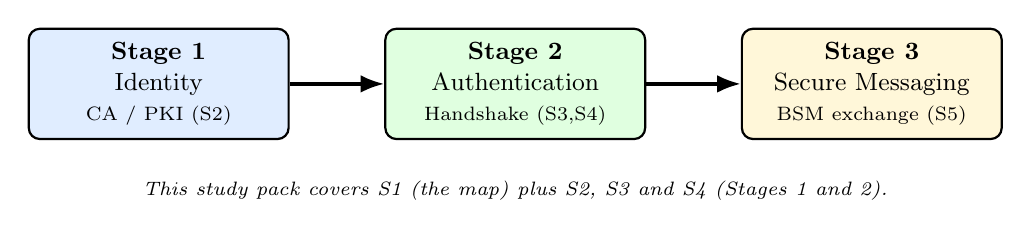
\begin{tikzpicture}[node distance=10mm and 12mm,
    every node/.style={font=\small},
    stage/.style={draw,rounded corners,minimum width=3.3cm,minimum height=1.4cm,
                  align=center,thick}]
  \node[stage,fill=boxblue]   (id)   {\textbf{Stage 1}\\Identity\\\scriptsize CA / PKI (S2)};
  \node[stage,fill=green!12,right=of id]   (auth) {\textbf{Stage 2}\\Authentication\\\scriptsize Handshake (S3,S4)};
  \node[stage,fill=boxyellow,right=of auth] (msg) {\textbf{Stage 3}\\Secure Messaging\\\scriptsize BSM exchange (S5)};
  \draw[-{Latex[length=3mm]},very thick] (id)   -- (auth);
  \draw[-{Latex[length=3mm]},very thick] (auth) -- (msg);
  \node[below=4mm of auth,font=\scriptsize\itshape,align=center]
       {This study pack covers S1 (the map) plus S2, S3 and S4 (Stages 1 and 2).};
\end{tikzpicture}
\end{center}

% =====================================================================
\section{The Theory You Must Study}
% =====================================================================

\subsection{Vehicle-to-Vehicle (V2V) Communication}
\textbf{Plain definition.} V2V communication means cars wirelessly broadcasting
short messages to nearby cars about their position, speed and movement, so the
cars (or their drivers) can react to danger faster than a human could.

\textbf{Real-life analogy.} Imagine every car has a loudspeaker on its roof
constantly calling out ``I am here, going 80, turning left''. Other cars hear
this and brake or steer in time.

\textbf{Why it exists / what problem it solves.} Human reaction time is slow and
a driver cannot see around a blind corner or through the truck in front. V2V
lets a car ``see'' a sudden brake three vehicles ahead and react in
milliseconds, preventing pile-ups.

\textbf{How it works at a beginner level.} Each car has a small radio. Several
times every second it sends a tiny message. Nearby cars receive it and update
their picture of the traffic around them. \emph{In this project the radio is
simulated by an ordinary TCP network connection between two programs.}

\textbf{Security property it relates to.} None on its own --- V2V is just the
\emph{communication}. The danger is precisely that, by default, this
communication has \emph{no} security at all. Everything else in the project
exists to add security on top.

\subsection{Basic Safety Message (BSM)}
\textbf{Plain definition.} A BSM is the small data packet a vehicle broadcasts.
It contains facts such as speed, heading (which way the car points), location,
and whether the brakes are on.

\textbf{Real-life analogy.} A BSM is like a quick status shout: ``Speed 80,
heading 45 degrees, not braking.'' It is short, said often, and instantly
forgotten once newer information arrives.

\textbf{Why it exists.} Cars need a \emph{standard, tiny} message so the radio
channel is not flooded and every car understands every other car. Real systems
(the SAE~J2735 standard) broadcast a BSM about ten times per second.

\textbf{How it works here.} In this project the readme states a BSM is sent
\emph{once per second} --- controlled by the constant
\texttt{BSM\_SEND\_INTERVAL = 1.0} in \texttt{config.py}. A BSM carries fields
like speed, heading and a braking flag. (Real V2V sends BSMs about ten times a
second; the project slows this to once a second so a human watching the
dashboard can follow along. This is a deliberate simplification.)

\textbf{Security property it relates to.} A BSM is the \emph{thing being
protected}. All six security properties below are promises about what happens
to a BSM as it crosses the network.

\subsection{The Untrusted Channel and the Threat Model}
\textbf{Plain definition.} A \emph{threat model} is a clear written statement of
\emph{who might attack you} and \emph{what they are able to do}. An
\emph{untrusted channel} is a communication link you must assume the enemy
controls.

\textbf{Real-life analogy.} Posting a letter through a postal service run by
nosy, dishonest staff: they can read your letter, rewrite it, throw it away,
copy it and post the copy again next week, or even write a brand-new letter and
sign your name.

\textbf{Why it exists.} You cannot defend against an attacker you have not
described. The threat model forces the designer to be honest: ``assume the worst
about the network.''

\textbf{How it works here.} The readme's threat model assumes an attacker who
fully controls the channel between Vehicle~A and Vehicle~B. That attacker can:
\begin{itemize}
  \item \textbf{Eavesdrop} --- read every message that passes.
  \item \textbf{Tamper} --- change the contents of a message in transit.
  \item \textbf{Impersonate} --- pretend to be a legitimate vehicle.
  \item \textbf{Replay} --- record a real message and send it again later.
\end{itemize}
The project does \emph{not} try to defend against an attacker who has stolen a
vehicle's secret private key files from its hard disk, or against denial of
service (jamming the radio so no message gets through). Those are out of scope
--- a normal and honest limitation for a student project.

\textbf{Security property it relates to.} The threat model is the question;
the six security properties are the answer.

\subsection{The Four Attacks}

\subsubsection*{(a) Replay Attack}
\textbf{Definition.} The attacker copies a genuine, valid message and re-sends
the exact same bytes later.

\textbf{Analogy.} Recording someone saying ``open the door'' and playing the
recording back tomorrow to get in.

\textbf{The danger.} Re-sending an old ``I am braking hard!'' message could make
cars behind brake for no reason and cause a crash.

\textbf{Project defence.} Every message carries a \emph{timestamp}; messages
older than \texttt{TIMESTAMP\_MAX\_AGE = 5.0} seconds are rejected. Every message
also carries a one-time random number (a \emph{nonce}); once a nonce has been
seen it is remembered for \texttt{REPLAY\_WINDOW\_SECONDS = 300} seconds and any
repeat is rejected. Demo script: \texttt{attacks/replay\_attack.py}.

\subsubsection*{(b) Tamper Attack}
\textbf{Definition.} The attacker intercepts a message and changes part of it,
e.g. flips ``speed: 60'' to ``speed: 0''.

\textbf{Analogy.} Steaming open a sealed envelope, editing the letter inside,
and re-sealing it --- except here the seal is mathematical and cannot be faked.

\textbf{The danger.} False speed or position data makes other cars make wrong,
dangerous decisions.

\textbf{Project defence.} The encryption used, AES-256-GCM, produces a 128-bit
\emph{authentication tag} computed over the whole ciphertext. Changing even one
bit makes the tag mismatch and decryption fails immediately. Demo:
\texttt{attacks/tamper\_attack.py}.

\subsubsection*{(c) Man-in-the-Middle (MITM) Attack}
\textbf{Definition.} The attacker secretly sits between A and B, relaying (and
possibly altering) every message, while each side believes it is talking
directly to the other.

\textbf{Analogy.} A dishonest interpreter standing between two people who do not
share a language: each trusts the interpreter completely, so the interpreter can
quietly change every sentence.

\textbf{The danger.} The attacker could read or rewrite the entire conversation.

\textbf{Project defence.} Two layers. (Scenario~A) If the attacker offers a
\emph{fake certificate}, it is rejected because it is not signed by the trusted
CA. (Scenario~B) If the attacker tries to \emph{forge a signature}, it fails
because they do not own the vehicle's private key. Demo:
\texttt{attacks/mitm\_attack.py}.

\subsubsection*{(d) Impersonation / Spoofing}
\textbf{Definition.} The attacker pretends to be Vehicle~A without being
Vehicle~A.

\textbf{Analogy.} A stranger walking up to a border using a passport with
someone else's name on it.

\textbf{The danger.} A fake car could inject false safety messages and direct
real cars into danger.

\textbf{Project defence.} Each real vehicle has a certificate signed by the CA
\emph{and} a private key that only it owns. During the handshake a vehicle must
sign a fresh random challenge; only the true owner of the private key can
produce a signature that verifies. Impersonation overlaps with MITM Scenario~B
and is handled by the same handshake (Section~S4).

\subsection{The Six Security Properties}
A ``security property'' is a promise the system keeps. Table~\ref{tab:props}
lists the six the project claims, exactly as written in the readme.

\begin{table}[h]
\centering
\small
\begin{tabular}{@{}p{2.9cm} p{5.0cm} p{5.6cm}@{}}
\toprule
\textbf{Property} & \textbf{Plain meaning} & \textbf{How the project achieves it}\\
\midrule
Confidentiality & Only the intended car can read the message. &
AES-256-GCM encryption with a shared session key.\\
Integrity & The message cannot be changed without it being noticed. &
The 128-bit AES-GCM authentication tag.\\
Authentication & Each car proves who it really is. &
X.509 certificates plus the 4-step handshake.\\
Non-repudiation & A sender cannot later deny it sent the message. &
An ECDSA digital signature on every BSM.\\
Forward secrecy & Stealing a key tomorrow does not unlock today's messages. &
Fresh (ephemeral) ECDH keys generated per session.\\
Replay prevention & An old message cannot be reused. &
Nonce cache plus a 5-second timestamp window.\\
\bottomrule
\end{tabular}
\caption{The six security properties promised by the V2V project.}
\label{tab:props}
\end{table}

\textbf{One honest clarification about ``5 seconds''.} The readme's property
table summarises replay prevention as a ``5s window'', but the code actually
uses \emph{two} separate windows, and it helps to keep them apart:
\begin{itemize}
  \item \texttt{TIMESTAMP\_MAX\_AGE = 5.0} --- a message whose timestamp is more
        than 5~seconds away from ``now'' is rejected as \emph{stale}.
  \item \texttt{REPLAY\_WINDOW\_SECONDS = 300} --- each nonce that has been seen
        is \emph{remembered} for 300~seconds (5~minutes), so an exact repeat
        within that window is caught even if its timestamp were somehow fresh.
\end{itemize}
Together they form a belt-and-braces defence: the timestamp catches \emph{old}
messages cheaply, and the nonce cache catches \emph{exact duplicates}.

% =====================================================================
\section{Code Walkthrough}
% =====================================================================

Section~S1 has no large algorithm to trace. Its ``code'' is the project's
shared settings file, \texttt{config.py}. Every other module imports its numbers
from here so that there is a single, easy-to-find place to change behaviour.
Below is the real file, followed by a step-by-step explanation of every group.

\begin{lstlisting}[style=py,caption={config.py --- shared constants for the
whole simulation (decorative dashes in the original comments shortened to
plain ASCII for printing).}]
"""Shared configuration constants for the V2V security simulation."""

# -- Network Configuration --
VEHICLE_A_PORT = 9001          # TCP port Vehicle A listens on
VEHICLE_B_PORT = 9002          # TCP port Vehicle B listens on
DASHBOARD_A_PORT = 5001        # Flask dashboard for Vehicle A
DASHBOARD_B_PORT = 5002        # Flask dashboard for Vehicle B

# -- Certificate Paths --
CA_CERT_PATH = "ca/certs/ca_cert.pem"
CA_KEY_PATH = "ca/certs/ca_key.pem"
VEHICLE_A_CERT = "ca/certs/vehicle-a_cert.pem"
VEHICLE_A_KEY = "ca/certs/vehicle-a_key.pem"
VEHICLE_B_CERT = "ca/certs/vehicle-b_cert.pem"
VEHICLE_B_KEY = "ca/certs/vehicle-b_key.pem"

# -- Security Parameters --
REPLAY_WINDOW_SECONDS = 300    # Nonces remembered for 5 minutes
TIMESTAMP_MAX_AGE = 5.0        # Messages older than 5 seconds are rejected
BSM_SEND_INTERVAL = 1.0        # Send a BSM every 1 second

# -- Crypto Settings --
AES_KEY_LENGTH = 32            # 256 bits (AES-256)
NONCE_LENGTH = 12              # 96 bits (AES-GCM standard nonce size)
EC_CURVE = "secp256r1"         # NIST P-256 curve (same as TLS 1.3)
SESSION_KEY_INFO = b"v2v-session-key-v1"  # HKDF info string

# -- Simulation Settings --
SIMULATED_LATITUDE = 6.9271    # Colombo, Sri Lanka
SIMULATED_LONGITUDE = 79.8612
SPEED_RANGE = (60.0, 100.0)    # km/h for simulated vehicle
\end{lstlisting}

\subsection{Group 1 --- Network Configuration}
\textbf{Purpose:} tells each program which ``door numbers'' (TCP ports) to use.
\begin{enumerate}
  \item A \emph{port} is a numbered door on a computer; a program listens behind
        one door so messages can find it.
  \item \texttt{VEHICLE\_A\_PORT = 9001} and \texttt{VEHICLE\_B\_PORT = 9002}:
        the two cars listen on ports 9001 and 9002.
  \item \texttt{DASHBOARD\_A\_PORT = 5001} and \texttt{DASHBOARD\_B\_PORT = 5002}:
        each car also runs a small web page (the dashboard) on its own port so
        you can watch it in a browser.
\end{enumerate}
\emph{Analogy:} ports are flat numbers in an apartment block --- the building
(computer) has one street address (IP), but the postman needs the flat number
to deliver to the right resident.

\subsection{Group 2 --- Certificate Paths}
\textbf{Purpose:} the file locations of every digital passport and key.
\begin{enumerate}
  \item \texttt{CA\_CERT\_PATH} / \texttt{CA\_KEY\_PATH}: the trusted authority's
        public certificate and its secret signing key.
  \item \texttt{VEHICLE\_A\_CERT} / \texttt{VEHICLE\_A\_KEY} (and the B pair):
        each vehicle's own passport and matching private key.
  \item All files end in \texttt{.pem}. PEM (Privacy-Enhanced Mail) is just a
        text format for storing keys and certificates --- you will meet it in
        detail in Section~S2.
\end{enumerate}
\emph{Tie to theory:} this group is the ``Identity'' stage on paper --- it
records where the passports live.

\subsection{Group 3 --- Security Parameters}
\textbf{Purpose:} the timing rules that stop replay attacks.
\begin{enumerate}
  \item \texttt{REPLAY\_WINDOW\_SECONDS = 300}: how long a used nonce is
        remembered. Implements the \emph{nonce cache} part of replay prevention.
  \item \texttt{TIMESTAMP\_MAX\_AGE = 5.0}: how stale a message may be before it
        is thrown away. Implements the \emph{freshness} part of replay
        prevention.
  \item \texttt{BSM\_SEND\_INTERVAL = 1.0}: send one safety message per second.
\end{enumerate}
\emph{Tie to theory:} this group is the numeric heart of the
\textbf{replay prevention} property.

\subsection{Group 4 --- Crypto Settings}
\textbf{Purpose:} the sizes and names of the cryptographic building blocks.
\begin{enumerate}
  \item \texttt{AES\_KEY\_LENGTH = 32}: the secret key is 32 bytes = 256 bits,
        hence ``AES-256''. Implements \textbf{confidentiality}.
  \item \texttt{NONCE\_LENGTH = 12}: the AES-GCM nonce is 12 bytes = 96 bits,
        the size recommended by the standard. (Note: this is the encryption
        nonce. The handshake in S4 uses a separate, larger 32-byte nonce ---
        do not confuse the two.)
  \item \texttt{EC\_CURVE = "secp256r1"}: the name of the elliptic curve used
        for keys --- the same NIST P-256 curve used by TLS~1.3 (the protocol
        behind HTTPS).
  \item \texttt{SESSION\_KEY\_INFO = b"v2v-session-key-v1"}: a label fed into the
        key-derivation step (HKDF) so the derived key is tied to this exact
        purpose.
\end{enumerate}
\emph{Honest note on accuracy:} \texttt{config.py} is meant to be the single
source of truth, but a few modules hard-code the same values directly instead of
importing them --- for example \texttt{crypto/crypto.py} writes
\texttt{os.urandom(12)} and the literal string \texttt{b"v2v-session-key-v1"}
itself rather than reading \texttt{NONCE\_LENGTH} and \texttt{SESSION\_KEY\_INFO}.
The numbers agree, so behaviour is correct, but it is good practice to notice
this duplication and mention it if an examiner asks ``is config.py actually
used everywhere?''

\subsection{Group 5 --- Simulation Settings}
\textbf{Purpose:} fake but realistic data so the cars have something to ``say''.
\begin{enumerate}
  \item \texttt{SIMULATED\_LATITUDE} / \texttt{SIMULATED\_LONGITUDE}: a fixed GPS
        location (Colombo, Sri Lanka) used as the starting point.
  \item \texttt{SPEED\_RANGE = (60.0, 100.0)}: the simulated car picks a speed
        between 60 and 100 km/h.
\end{enumerate}
\emph{Tie to theory:} this is the \emph{content of a BSM} --- the very data the
six security properties are protecting.

\medskip
\noindent\textbf{Why a config file at all?} If the port number or the timeout
were scattered across ten files, changing one would mean ten risky edits.
Centralising them is the same idea as a fuse box: all the switches in one labelled
panel. There are no function arguments, return values, or exceptions in
\texttt{config.py} --- it is pure data, executed once when imported.

% =====================================================================
\section{Hands-On / Practical}
% =====================================================================

S1 is the ``map'' section, so the practical work is to (1) confirm your tools
are installed, (2) inspect the shared settings, and (3) see the whole pipeline
run once end to end.

\subsection{Step 1 --- Check Python and the crypto library}
Open PowerShell in the project folder and run:
\begin{lstlisting}[style=term]
python --version
pip install cryptography flask requests pytest
\end{lstlisting}
You need Python 3.10 or newer. The \texttt{cryptography} library supplies all
the encryption maths used by S3 and S4.

\subsection{Step 2 --- Inspect the shared constants}
Run a one-line Python command that imports \texttt{config.py} and prints a few
values:
\begin{lstlisting}[style=term]
python -c "import config; print(config.AES_KEY_LENGTH, config.TIMESTAMP_MAX_AGE, config.BSM_SEND_INTERVAL)"
\end{lstlisting}

\noindent\textbf{Expected output:}
\begin{lstlisting}[style=term]
32 5.0 1.0
\end{lstlisting}
\textbf{What each number means:} \texttt{32} is the AES key length in bytes (a
256-bit key); \texttt{5.0} is the maximum age in seconds before a message is
treated as stale; \texttt{1.0} is the gap in seconds between safety messages.

\subsection{Step 3 --- Watch the whole pipeline once}
You can see all three stages in a single run by generating the certificates and
running the handshake demo (these belong to S2--S4 but together they show the
S1 big picture):
\begin{lstlisting}[style=term]
python ca\ca.py
python ca\issue_cert.py --vehicle-id vehicle-a --output-dir ca\certs
python ca\issue_cert.py --vehicle-id vehicle-b --output-dir ca\certs
python protocol\auth_protocol.py
\end{lstlisting}
The first three commands build Stage~1 (Identity); the last command runs
Stage~2 (Authentication) and ends by printing that both cars derived the
\emph{same} session key.

\subsection{Try This Yourself (mini-experiment)}
Open \texttt{config.py} and change one line:
\begin{lstlisting}[style=term]
TIMESTAMP_MAX_AGE = 5.0      ->   TIMESTAMP_MAX_AGE = 0.001
\end{lstlisting}
\textbf{Predict before you run.} 0.001~seconds is one millisecond. A message
almost always takes longer than a millisecond to build and travel, so by the
time it is checked it is already ``too old''. Prediction: the handshake or BSM
exchange should now \emph{fail} with a ``stale message'' error, even though
nothing malicious happened. This shows that security parameters are a balance ---
too strict and the honest system breaks; too loose and attacks slip through.
\textbf{Remember to change the value back to 5.0 afterwards.}

% =====================================================================
\section{Attack Relevance}
% =====================================================================

S1 does not itself contain a defence --- it is the chapter that \emph{names} the
attacks and the defences so the rest of the project has a target. Still, it is
directly relevant to all four attacks because it defines them and points to the
file that demonstrates each one.

\begin{table}[h]
\centering
\small
\begin{tabular}{@{}p{2.6cm} p{5.6cm} p{5.3cm}@{}}
\toprule
\textbf{Attack} & \textbf{What the attacker does} & \textbf{Which property/section stops it}\\
\midrule
Replay & Re-sends a captured valid message. &
Replay prevention --- timestamp + nonce cache (S4).\\
Tamper & Edits a message in transit. &
Integrity --- AES-GCM authentication tag (S3, S5).\\
MITM & Relays/alters traffic from the middle. &
Authentication --- certificates + handshake (S2, S4).\\
Impersonation & Pretends to be a real vehicle. &
Authentication + non-repudiation --- signed challenge (S2, S4).\\
\bottomrule
\end{tabular}
\caption{S1 maps each attack to the property and section that defeats it.}
\end{table}

\noindent The \texttt{config.py} constants \texttt{TIMESTAMP\_MAX\_AGE} and
\texttt{REPLAY\_WINDOW\_SECONDS} are the only S1 items that play a \emph{direct}
defensive role: they are the dials that tune how aggressively replay attacks are
rejected.

% =====================================================================
\section{Illustrations}
% =====================================================================

\subsection{Diagram 1 --- The Threat Model}
The attacker owns the channel. Figure below shows the honest vehicles at the
edges and the attacker controlling everything in between.

\begin{center}
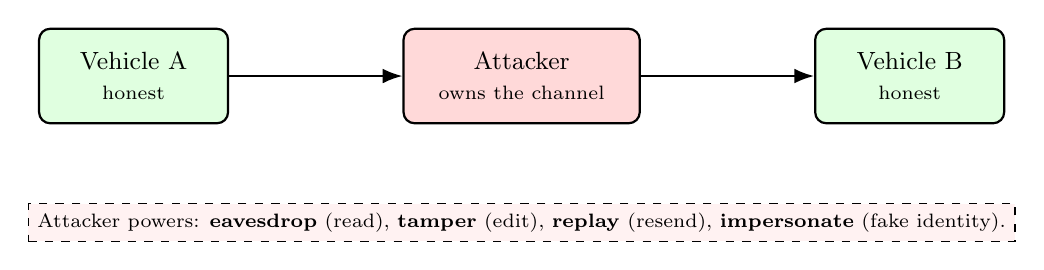
\begin{tikzpicture}[node distance=8mm,font=\small,
   car/.style={draw,thick,rounded corners,fill=green!12,minimum width=2.4cm,
               minimum height=1.2cm,align=center},
   atk/.style={draw,thick,rounded corners,fill=red!15,minimum width=3.0cm,
               minimum height=1.2cm,align=center}]
  \node[car] (a) {Vehicle A\\\scriptsize honest};
  \node[atk,right=22mm of a] (m) {Attacker\\\scriptsize owns the channel};
  \node[car,right=22mm of m] (b) {Vehicle B\\\scriptsize honest};
  \draw[-{Latex[length=2.5mm]},thick] (a) -- (m);
  \draw[-{Latex[length=2.5mm]},thick] (m) -- (b);
  \node[below=10mm of m,align=center,font=\scriptsize,draw,dashed,fill=red!5,
        minimum width=8.5cm]
       {Attacker powers: \textbf{eavesdrop} (read), \textbf{tamper} (edit),
        \textbf{replay} (resend), \textbf{impersonate} (fake identity).};
\end{tikzpicture}
\end{center}

\subsection{Diagram 2 --- The Three-Stage Pipeline with Files}
\begin{center}
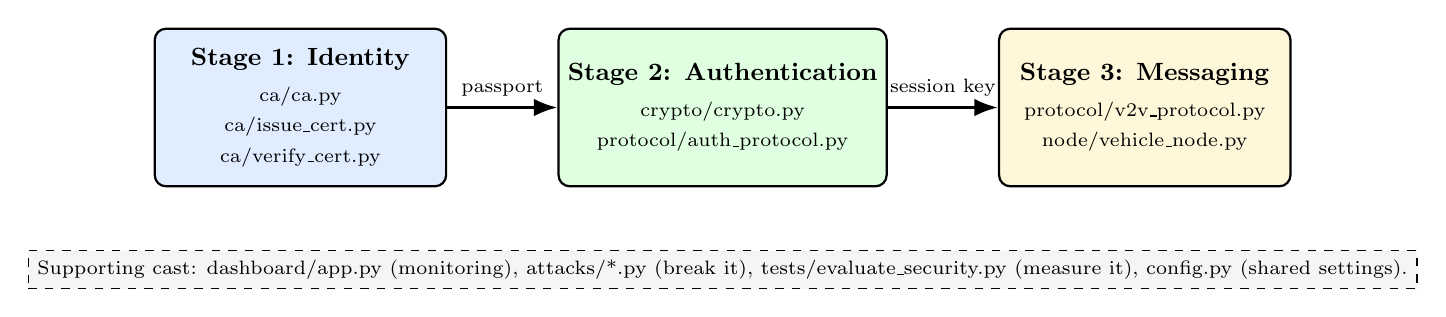
\begin{tikzpicture}[font=\small,node distance=6mm,
   box/.style={draw,rounded corners,minimum width=3.7cm,minimum height=2.0cm,
               align=center,thick}]
  \node[box,fill=boxblue]   (s1) {\textbf{Stage 1: Identity}\\[2pt]
        \scriptsize ca/ca.py\\\scriptsize ca/issue\_cert.py\\\scriptsize ca/verify\_cert.py};
  \node[box,fill=green!12,right=14mm of s1] (s2)
       {\textbf{Stage 2: Authentication}\\[2pt]
        \scriptsize crypto/crypto.py\\\scriptsize protocol/auth\_protocol.py};
  \node[box,fill=boxyellow,right=14mm of s2] (s3)
       {\textbf{Stage 3: Messaging}\\[2pt]
        \scriptsize protocol/v2v\_protocol.py\\\scriptsize node/vehicle\_node.py};
  \draw[-{Latex[length=3mm]},very thick] (s1) -- (s2)
       node[midway,above,font=\scriptsize]{passport};
  \draw[-{Latex[length=3mm]},very thick] (s2) -- (s3)
       node[midway,above,font=\scriptsize]{session key};
  \node[below=8mm of s2,draw,dashed,fill=gray!8,minimum width=11cm,
        align=center,font=\scriptsize]
       {Supporting cast: dashboard/app.py (monitoring), attacks/*.py (break it),
        tests/evaluate\_security.py (measure it), config.py (shared settings).};
\end{tikzpicture}
\end{center}

% =====================================================================
\section{Presentation Pack}
% =====================================================================

\subsection{Slide Outline}

\textbf{Slide 1 --- The Problem.}
\begin{itemize}
  \item Cars send tiny ``safety messages'' (BSMs) many times a second.
  \item The radio channel is untrusted --- anyone nearby can listen.
  \item No security by default: a stranger can read, change, copy or fake messages.
  \item One false ``I am braking'' message could cause a crash.
\end{itemize}

\textbf{Slide 2 --- The Threat Model (who is the enemy?).}
\begin{itemize}
  \item We assume the attacker fully controls the channel.
  \item Four powers: eavesdrop, tamper, replay, impersonate.
  \item Out of scope: stealing key files from a car, jamming the radio.
  \item ``Design for the worst attacker you can describe.''
\end{itemize}

\textbf{Slide 3 --- The Four Attacks.}
\begin{itemize}
  \item Replay --- resend an old valid message.
  \item Tamper --- edit a message in transit.
  \item MITM --- secretly relay/alter the whole conversation.
  \item Impersonation --- pretend to be a real vehicle.
  \item Each has a demo script in the \texttt{attacks/} folder.
\end{itemize}

\textbf{Slide 4 --- The Six Security Properties.}
\begin{itemize}
  \item Confidentiality, Integrity, Authentication.
  \item Non-repudiation, Forward secrecy, Replay prevention.
  \item Each property is a \emph{promise} kept by a specific technique.
  \item Show Table~\ref{tab:props} on screen.
\end{itemize}

\textbf{Slide 5 --- The Three-Stage Pipeline.}
\begin{itemize}
  \item Stage 1 Identity --- give every car a passport (CA).
  \item Stage 2 Authentication --- handshake to prove identity + share a key.
  \item Stage 3 Secure Messaging --- sign then encrypt every BSM.
  \item \texttt{config.py} is the shared settings file feeding all three.
\end{itemize}

\subsection{Speaker Talking Points (about 30--60 seconds each)}

\textbf{Slide 1.} ``Picture two cars on a highway. Modern cars can talk to each
other by radio, sending tiny status messages called Basic Safety Messages many
times a second --- speed, direction, braking. This is genuinely useful: a car
can warn the car behind it before a human even notices danger. But the radio
link is open air. Anyone with a receiver can join in. If we send these messages
with no protection, a stranger can read them, change them, or fake them --- and
a single false `I am braking hard' message could trigger a real crash. So the
project's job is to add a security layer.''

\textbf{Slide 2.} ``Before defending anything, a security engineer writes down
the threat model --- who the enemy is and what they can do. We make a deliberately
pessimistic assumption: the attacker completely owns the channel between the two
cars. They can listen to every message, change any message, copy a message and
send it again, or pretend to be one of the cars. We are honest about limits too:
we do not defend against someone physically stealing the secret key files from
inside a car, or jamming the radio entirely. Naming what you do not cover is part
of good security work.''

\textbf{Slide 3.} ``Those attacker powers turn into four concrete attacks. A
replay attack records a real message and plays it back later. A tamper attack
edits a message as it passes. A man-in-the-middle attack puts the attacker
secretly in the middle, like a dishonest interpreter relaying and changing every
sentence. And impersonation is simply pretending to be a car you are not. The
nice thing about this project is that each attack has its own script in the
attacks folder, so we can actually run the attack and watch it fail.''

\textbf{Slide 4.} ``For each attacker power we promise a security property.
Confidentiality means only the intended car can read the message. Integrity
means any change is detected. Authentication means each car proves who it is.
Non-repudiation means a sender cannot later deny what it sent. Forward secrecy
means that even if a key leaks tomorrow, today's messages stay secret. And replay
prevention means an old message cannot be reused. Six promises --- and every one
is kept by a specific, named technique we will see in later sections.''

\textbf{Slide 5.} ``Finally, the big picture. The system is a pipeline of three
stages. Stage one, Identity: a Certificate Authority gives every car a digital
passport. Stage two, Authentication: the two cars run a four-step handshake to
check passports and secretly agree on a shared key. Stage three, Secure
Messaging: every safety message is signed and then encrypted before it goes out.
One small file, config.py, holds the shared settings --- ports, timeouts, key
sizes --- so all three stages read the same numbers.''

\subsection{Live-Demo Script}
\begin{enumerate}
  \item \textbf{Show the settings.} Run
        \texttt{python -c "import config; print(config.TIMESTAMP\_MAX\_AGE)"}.
        Point at the \texttt{5.0} and say ``this is our replay-freshness dial.''
  \item \textbf{Show the project map.} Open the folder in the editor; point at
        the \texttt{ca/}, \texttt{crypto/}, \texttt{protocol/}, \texttt{attacks/}
        folders and link each to a stage.
  \item \textbf{Run the pipeline.} Execute the four commands from
        Hands-On Step~3. Point at the final line ``both vehicles share the same
        key'' --- that is the whole project working in miniature.
  \item \textbf{Optional break-it moment.} Edit \texttt{TIMESTAMP\_MAX\_AGE} to
        \texttt{0.001}, re-run the handshake, and point at the ``stale message''
        failure to show parameters matter. Restore it to \texttt{5.0}.
\end{enumerate}

\subsection{Examiner Q\&A}
\begin{enumerate}
  \item \textbf{Q: What is a BSM and how often is it sent here?}\\
        A: A Basic Safety Message --- a small packet with speed, heading,
        location and braking state. In this project it is sent once per second
        (\texttt{BSM\_SEND\_INTERVAL = 1.0}); real V2V sends about ten per
        second, slowed here so a human can follow the dashboard.
  \item \textbf{Q: What is a threat model and what is this project's?}\\
        A: A written statement of who attacks and what they can do. Here: an
        attacker who fully controls the channel and can eavesdrop, tamper,
        replay and impersonate. Out of scope: stolen key files and jamming.
  \item \textbf{Q: Name the four attacks and one defence for each.}\\
        A: Replay (timestamp + nonce cache), Tamper (AES-GCM auth tag), MITM
        (CA-signed certificates), Impersonation (signed challenge proving
        private-key ownership).
  \item \textbf{Q: Name the six security properties.}\\
        A: Confidentiality, integrity, authentication, non-repudiation, forward
        secrecy, replay prevention.
  \item \textbf{Q: Difference between confidentiality and integrity?}\\
        A: Confidentiality hides the content (attacker cannot \emph{read} it);
        integrity protects the content (attacker cannot \emph{change} it
        undetected). AES-256-GCM gives both at once.
  \item \textbf{Q: Why two replay windows --- 5 seconds and 300 seconds?}\\
        A: \texttt{TIMESTAMP\_MAX\_AGE} (5\,s) cheaply rejects old messages;
        \texttt{REPLAY\_WINDOW\_SECONDS} (300\,s) remembers each nonce so an
        exact duplicate is caught even within the freshness window. Two layers,
        belt and braces.
  \item \textbf{Q: What is the purpose of config.py?}\\
        A: A single, central place for shared constants (ports, timeouts, key
        sizes) so a setting is changed once, not in many files.
  \item \textbf{Q: Is this a complete, real V2V system?}\\
        A: No --- it is a faithful \emph{simulation}. Real V2V uses dedicated
        radio (DSRC/C-V2X) and broadcasts to many cars; this project uses TCP
        between two programs and slows the message rate. The cryptography,
        however, is the same industry-standard set used by TLS.
\end{enumerate}

% =====================================================================
\section{Glossary}
% =====================================================================
\begin{description}[style=nextline,leftmargin=0pt]
  \item[V2V] Vehicle-to-Vehicle: cars exchanging wireless messages directly.
  \item[BSM] Basic Safety Message: the small status packet a vehicle broadcasts.
  \item[Threat model] A written description of who might attack and what they can do.
  \item[Untrusted channel] A communication link assumed to be under attacker control.
  \item[Eavesdrop] To secretly read messages in transit.
  \item[Tamper] To change a message's contents in transit.
  \item[Replay attack] Re-sending a previously captured valid message.
  \item[MITM] Man-in-the-Middle: an attacker secretly relaying/altering traffic.
  \item[Impersonation] Pretending to be a legitimate party (spoofing identity).
  \item[Confidentiality] Property: only the intended recipient can read a message.
  \item[Integrity] Property: any change to a message is detected.
  \item[Authentication] Property: each party proves who it really is.
  \item[Non-repudiation] Property: a sender cannot later deny having sent a message.
  \item[Forward secrecy] Property: past messages stay secret even if a key leaks later.
  \item[Replay prevention] Property: an old message cannot be reused.
  \item[Nonce] ``Number used once'': a one-time random value that detects duplicates.
  \item[Timestamp] A recorded time, used here to reject stale messages.
  \item[CA] Certificate Authority: the trusted issuer of digital passports.
  \item[Certificate] A digital passport binding an identity to a public key.
  \item[PEM] A text file format for storing keys and certificates.
  \item[Port] A numbered ``door'' on a computer that a program listens behind.
  \item[TCP] Transmission Control Protocol: a reliable network connection type.
  \item[AES-256-GCM] The authenticated encryption algorithm used for confidentiality + integrity.
  \item[ECDSA] Elliptic Curve Digital Signature Algorithm: proves who wrote a message.
  \item[ECDH] Elliptic Curve Diffie-Hellman: lets two parties agree a shared secret.
  \item[HKDF] A function that turns a raw shared secret into a clean usable key.
  \item[Session key] A temporary secret key used to encrypt one conversation.
  \item[config.py] The project's shared-settings file.
\end{description}

% =====================================================================
\section{References and Further Study}
% =====================================================================
\begin{itemize}
  \item \textbf{V2V overview (NHTSA, US road-safety agency)} ---
        \url{https://www.nhtsa.gov/research-data/vehicle-vehicle-communication}\\
        Read for: why V2V exists and the real-world safety case.
  \item \textbf{Vehicular communication systems (Wikipedia)} ---
        \url{https://en.wikipedia.org/wiki/Vehicular_communication_systems}\\
        Read for: a plain-English overview of the whole field.
  \item \textbf{SAE J2735 message-set standard} ---
        \url{https://www.sae.org/standards/content/j2735_202309/}\\
        Read for: the real definition of the Basic Safety Message.
  \item \textbf{IEEE 1609.2 (security for V2X)} ---
        \url{https://standards.ieee.org/ieee/1609.2/10258/}\\
        Read for: how real V2V security and certificates work.
  \item \textbf{Information security / the CIA triad (Wikipedia)} ---
        \url{https://en.wikipedia.org/wiki/Information_security}\\
        Read for: confidentiality, integrity, availability explained.
  \item \textbf{Replay attack (Wikipedia)} ---
        \url{https://en.wikipedia.org/wiki/Replay_attack}\\
        Read for: how replay works and standard defences.
  \item \textbf{Man-in-the-middle attack (Wikipedia)} ---
        \url{https://en.wikipedia.org/wiki/Man-in-the-middle_attack}\\
        Read for: the MITM concept and why authentication stops it.
  \item \textbf{Non-repudiation (Wikipedia)} ---
        \url{https://en.wikipedia.org/wiki/Non-repudiation}\\
        Read for: why digital signatures give non-repudiation.
  \item \textbf{Forward secrecy (Wikipedia)} ---
        \url{https://en.wikipedia.org/wiki/Forward_secrecy}\\
        Read for: why ephemeral keys protect past sessions.
  \item \textbf{Threat modelling (OWASP)} ---
        \url{https://owasp.org/www-community/Threat_Modeling}\\
        Read for: how professionals build a threat model.
  \item \textbf{NIST Computer Security Resource Center glossary} ---
        \url{https://csrc.nist.gov/glossary}\\
        Read for: precise definitions of every security term.
  \item \textbf{Python cryptography library documentation} ---
        \url{https://cryptography.io/en/latest/}\\
        Read for: the library this whole project is built on (used heavily in S2--S5).
\end{itemize}

\vfill
\begin{center}\footnotesize\itshape
End of Section S1. Next: S2 --- Public Key Infrastructure / Certificate Authority.
\end{center}



% ===================== 02-pki-certificate-authority.tex =====================
\chapter{S2 --- Public Key Infrastructure and the Certificate Authority}

\section{Title and ``What You'll Learn''}
% =====================================================================

\subsection*{Section Title}
\textbf{S2 --- The Public Key Infrastructure (PKI): how the project creates a
trusted ``passport office'' and issues digital passports to vehicles.}

\subsection*{Plain-English Summary (read this first)}
Before two cars can trust each other, each one needs a digital \emph{identity}
that cannot be faked. Section~S2 builds that identity system. A special program,
the \textbf{Certificate Authority (CA)}, acts like a passport office: it creates
its own master signing key and a self-signed master certificate, and then
\emph{signs} a small certificate for each vehicle. Any car can later check
another car's certificate by verifying the CA's signature on it --- if the CA
did not sign it, it is a fake. Three Python files do this work: \texttt{ca.py}
creates the CA, \texttt{issue\_cert.py} signs a certificate for one vehicle, and
\texttt{verify\_cert.py} checks a certificate.

\subsection*{Learning Outcomes}
After studying this section you will be able to:
\begin{itemize}
  \item Explain what \textbf{public-key (asymmetric) cryptography} is and why a
        key comes in a public/private pair.
  \item Explain \textbf{elliptic-curve cryptography} and the NIST \textbf{P-256}
        curve at a beginner level.
  \item Explain \textbf{SHA-256 hashing} and \textbf{ECDSA digital signatures}.
  \item Describe an \textbf{X.509 certificate}, its main fields, and the
        \textbf{BasicConstraints} and \textbf{KeyUsage} extensions.
  \item Explain \textbf{PEM, DER and Base64} encodings.
  \item Explain \textbf{PKI}, the \textbf{chain of trust}, a \textbf{trust
        anchor}, and a \textbf{self-signed root}.
  \item Walk through every function in \texttt{ca.py}, \texttt{issue\_cert.py}
        and \texttt{verify\_cert.py} and say what each line does.
  \item Run the three scripts, read their output, and explain how this stage
        defeats a man-in-the-middle attacker using a forged certificate.
\end{itemize}

% =====================================================================
\section{Where This Fits}
% =====================================================================

S2 is \textbf{Stage~1: Identity} of the three-stage pipeline. It comes first
because authentication (Stage~2) and secure messaging (Stage~3) are both built
\emph{on top of} the certificates created here. The handshake in S4 does not
re-invent identity --- it simply calls a verification routine that checks the
certificates this section produced.

\begin{center}
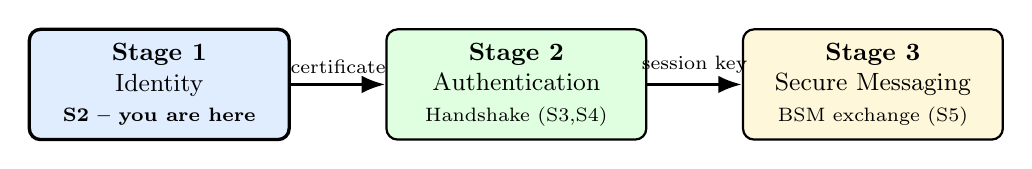
\begin{tikzpicture}[node distance=10mm and 12mm,every node/.style={font=\small},
    stage/.style={draw,rounded corners,minimum width=3.3cm,minimum height=1.4cm,
                  align=center,thick}]
  \node[stage,fill=boxblue,very thick]   (id)   {\textbf{Stage 1}\\Identity\\\scriptsize \textbf{S2 -- you are here}};
  \node[stage,fill=green!12,right=of id]   (auth) {\textbf{Stage 2}\\Authentication\\\scriptsize Handshake (S3,S4)};
  \node[stage,fill=boxyellow,right=of auth] (msg) {\textbf{Stage 3}\\Secure Messaging\\\scriptsize BSM exchange (S5)};
  \draw[-{Latex[length=3mm]},very thick] (id)   -- (auth)
       node[midway,above,font=\scriptsize]{certificate};
  \draw[-{Latex[length=3mm]},very thick] (auth) -- (msg)
       node[midway,above,font=\scriptsize]{session key};
\end{tikzpicture}
\end{center}

\noindent The \emph{certificate} produced here is the bridge into Stage~2: the
handshake hands a certificate to the other vehicle as proof of identity.

% =====================================================================
\section{The Theory You Must Study}
% =====================================================================

\subsection{Symmetric vs Asymmetric (Public-Key) Cryptography}
\textbf{Plain definition.} \emph{Symmetric} cryptography uses \emph{one} secret
key for both locking and unlocking --- both sides must already share it.
\emph{Asymmetric} (or \emph{public-key}) cryptography uses a \emph{pair} of
keys: a \textbf{private key} kept secret, and a \textbf{public key} given to
everyone. What one key does, only the other can undo.

\textbf{Real-life analogy.} Symmetric is one house key that both you and your
flatmate carry. Asymmetric is a mailbox: anyone can drop a letter through the
public slot, but only you have the private key to open the box and read it.

\textbf{Why it exists.} Symmetric keys have a chicken-and-egg problem: how do two
strangers agree on a shared secret over an untrusted channel \emph{without}
already having a secret? Public-key cryptography solves this --- you can publish
your public key to the whole world and it is still safe.

\textbf{How it works here.} Every key in S2 is a public/private \emph{pair}. The
CA has a pair; each vehicle has a pair. The private key is used to \emph{sign};
the public key is used to \emph{verify}. The certificate is simply a wrapper
that publishes a public key together with a name.

\textbf{Security property it provides.} Public-key cryptography underpins
\textbf{authentication} and \textbf{non-repudiation}.

\subsection{Elliptic-Curve Cryptography (ECC) and the P-256 Curve}
\textbf{Plain definition.} ECC is a family of public-key algorithms whose
security comes from the difficulty of a particular kind of arithmetic done on a
curved mathematical shape called an \emph{elliptic curve}.

\textbf{Real-life analogy.} Think of points hopping around a closed loop
according to a fixed rule. Going \emph{forwards} a known number of hops is easy;
working out \emph{how many hops} someone took just by seeing where they landed
is practically impossible. The private key is ``the number of hops''; the public
key is ``where you landed''.

\textbf{Why it exists.} An older algorithm, RSA, needs very large keys (2048+
bits) for strong security. ECC reaches the same strength with much smaller keys
(256 bits) --- so it is faster and the certificates and signatures are smaller,
which matters for cars sending messages many times a second.

\textbf{How it works here.} The project uses the curve named \texttt{SECP256R1},
also called \textbf{NIST P-256}. Both \texttt{ca.py} and \texttt{issue\_cert.py}
call \texttt{generate\_private\_key(SECP256R1())} to create keys on this curve.
P-256 gives a ``128-bit security level'' --- strong enough for decades --- and
it is the same curve used by TLS~1.3 (the security behind HTTPS).

\textbf{Security property it provides.} ECC is the engine under
\textbf{authentication} (via ECDSA signatures) and the key exchange in S3/S4.

\subsection{SHA-256 Hashing}
\textbf{Plain definition.} A \emph{hash function} takes any amount of data and
produces a short, fixed-size fingerprint of it. SHA-256 always produces 256 bits
(32 bytes). The same input always gives the same fingerprint; changing one bit
of input changes the fingerprint completely and unpredictably.

\textbf{Real-life analogy.} A paper shredder that always outputs the same-size
pile of confetti --- but a magic one, where identical documents always give an
identical pile, and you cannot rebuild the document from the confetti.

\textbf{Why it exists.} It is far faster to sign or compare a tiny 32-byte
fingerprint than a huge document, and the fingerprint reliably represents the
whole document.

\textbf{How it works here.} When the CA signs a certificate it does not sign the
raw certificate bytes directly --- it signs their SHA-256 hash. The code shows
this as \texttt{algorithm=hashes.SHA256()} passed to the \texttt{sign} call, and
\texttt{issue\_cert.py} also uses SHA-256 to compute a human-readable
\emph{fingerprint} of the finished certificate.

\textbf{Security property it provides.} Hashing supports \textbf{integrity}: any
change to the certificate changes its hash, so the signature no longer matches.

\subsection{Digital Signatures and ECDSA}
\textbf{Plain definition.} A digital signature is a short value, produced with a
\emph{private} key, that anyone holding the matching \emph{public} key can check.
ECDSA (Elliptic Curve Digital Signature Algorithm) is the elliptic-curve version.

\textbf{Real-life analogy.} A wax seal on a letter. Only the owner of the unique
seal-ring (private key) can press a genuine seal; anyone can look at the seal and
recognise it (public key) without owning the ring.

\textbf{Why it exists.} It answers two questions at once: ``who really wrote
this?'' (authentication) and ``has it been changed since?'' (integrity) --- and
because only the owner could have signed it, they cannot later deny it
(non-repudiation).

\textbf{How it works here.} \emph{Signing:} the CA computes the SHA-256 hash of
the certificate body and, using its private key and the P-256 curve, produces a
signature. \emph{Verifying:} a vehicle takes the certificate body, re-hashes it,
and uses the CA's \emph{public} key to confirm the signature matches. In
\texttt{verify\_cert.py} this is the line
\texttt{ca\_public\_key.verify(certificate.signature,
certificate.tbs\_certificate\_bytes, ec.ECDSA(...))}.

\textbf{Security property it provides.} \textbf{Authentication},
\textbf{integrity} and \textbf{non-repudiation}.

\subsection{X.509 Certificates}
\textbf{Plain definition.} An X.509 certificate is a standard-format digital
document that \emph{binds} a public key to an identity, and is \emph{signed} by
an issuer so others can trust the binding.

\textbf{Real-life analogy.} A passport. It contains your photo and name (the
identity), is printed in a worldwide standard format, and carries the issuing
government's tamper-proof features (the signature). A passport with no government
features is just a booklet --- worthless.

\textbf{Why it exists.} A bare public key is just a number --- it does not say
\emph{whose} key it is. The certificate attaches a name (``vehicle-a'') to the
key and has a trusted party vouch for that attachment.

\textbf{How it works here.} A certificate in this project contains:
\begin{itemize}
  \item \textbf{Subject} --- who the certificate is about (e.g.\ Common Name
        \texttt{vehicle-a}, Organisation \texttt{V2V-Security-Lab}).
  \item \textbf{Issuer} --- who signed it (the CA, \texttt{V2V-Root-CA}).
  \item \textbf{Public key} --- the subject's P-256 public key.
  \item \textbf{Serial number} --- a unique random number for this certificate.
  \item \textbf{Validity period} --- ``not valid before'' and ``not valid
        after'' dates.
  \item \textbf{Extensions} --- extra rules: BasicConstraints and KeyUsage.
  \item \textbf{Signature} --- the issuer's ECDSA signature over all of the above.
\end{itemize}

\textbf{Security property it provides.} The foundation of \textbf{authentication}.

\subsection{Certificate Extensions: BasicConstraints and KeyUsage}
\textbf{Plain definition.} Extensions are extra fields that state \emph{rules}
about how a certificate may be used. Each extension can be marked
\textbf{critical}, meaning a verifier that does not understand it must reject the
certificate.

\textbf{BasicConstraints} answers: ``Is this a Certificate Authority?''
\begin{itemize}
  \item For the CA: \texttt{ca=True} --- yes, it is allowed to sign \emph{other}
        certificates.
  \item For a vehicle: \texttt{ca=False} --- no, a vehicle may not sign
        certificates for anyone else.
\end{itemize}

\textbf{KeyUsage} answers: ``What is this key allowed to do?''
\begin{itemize}
  \item For the CA: \texttt{key\_cert\_sign=True} --- the only thing the CA key
        may do is sign certificates.
  \item For a vehicle: \texttt{digital\_signature=True} --- the vehicle key may
        sign data (used later in the handshake and BSM signing).
\end{itemize}

\textbf{Real-life analogy.} BasicConstraints is the difference between a
\emph{passport office} (may issue passports) and a \emph{citizen} (may not).
KeyUsage is like a driving licence that says ``car only, not motorbike''.

\textbf{Why it exists.} Without these limits, a stolen vehicle certificate could
be abused to issue fake certificates for a whole fleet. The constraints box each
key into exactly one job.

\textbf{Security property it provides.} It strengthens \textbf{authentication}
by preventing privilege escalation (a vehicle pretending to be a CA).

\subsection{Encodings: Base64, DER and PEM}
\textbf{Plain definition.}
\begin{itemize}
  \item \textbf{DER} (Distinguished Encoding Rules) is the compact \emph{binary}
        form of a certificate or key --- raw bytes.
  \item \textbf{Base64} is a way of writing binary bytes using only 64 ordinary
        printable letters/digits, so binary survives being copied as text.
  \item \textbf{PEM} (Privacy-Enhanced Mail) wraps Base64 text between header and
        footer lines such as \texttt{-----BEGIN CERTIFICATE-----} and
        \texttt{-----END CERTIFICATE-----}.
\end{itemize}

\textbf{Real-life analogy.} DER is a delicate object; Base64 is bubble-wrapping
it so it travels safely; PEM is the labelled cardboard box with ``BEGIN'' and
``END'' written on the flaps.

\textbf{Why it exists.} Binary bytes can be corrupted by e-mail, text editors or
copy-paste. PEM text survives all of that, and the BEGIN/END labels make it
obvious what is inside.

\textbf{How it works here.} Every file the CA writes ends in \texttt{.pem}. The
code calls \texttt{certificate.public\_bytes(serialization.Encoding.PEM)} and
\texttt{private\_key.private\_bytes(encoding=serialization.Encoding.PEM, ...)}.
When loading, it calls \texttt{x509.load\_pem\_x509\_certificate(...)}.

\textbf{Security property it provides.} None directly --- encoding is about
\emph{format}, not secrecy. (A PEM file is still readable; secrecy of a private
key comes from keeping the file itself protected.)

\subsection{PKI, the Chain of Trust, and the Self-Signed Root}
\textbf{Plain definition.} A \textbf{Public Key Infrastructure (PKI)} is the
whole system of authorities, certificates and rules that lets strangers trust
each other's public keys. A \textbf{chain of trust} is the line of signatures
from a certificate you are checking back to one you already trust. A
\textbf{trust anchor} (or \textbf{root}) is that already-trusted starting point.

\textbf{Real-life analogy.} You trust a stranger's passport because you trust the
\emph{country} that issued it --- you do not need to personally know the
stranger. The country is the trust anchor; the passport chains back to it.

\textbf{The self-signed root problem.} The CA is the top of the tree --- nobody
is above it to sign \emph{its} certificate. So the CA signs its own certificate
with its own private key: a \textbf{self-signed certificate}. Its ``issuer'' and
``subject'' are the same name. This is not a security trick; it simply means
``trust in this root must be established out-of-band'' --- you must obtain
\texttt{ca\_cert.pem} through a trusted route and decide to trust it. Every
vehicle is given a copy of \texttt{ca\_cert.pem} as its trust anchor.

\textbf{How it works here.} The chain in this project is exactly two links long:
\[
\texttt{V2V-Root-CA (self-signed)} \;\longrightarrow\;
\texttt{vehicle-a / vehicle-b certificate}.
\]
To trust a vehicle's certificate, you check one signature: ``did V2V-Root-CA
sign it?''

\textbf{Security property it provides.} The whole basis of
\textbf{authentication} and the defence against \textbf{MITM}.

\subsection{Serial Number and Fingerprint}
\textbf{Serial number.} A unique number the issuer puts inside each certificate
so it can be referred to and, if needed, revoked. The code uses
\texttt{x509.random\_serial\_number()} --- a large random number, so two
certificates practically never collide.

\textbf{Fingerprint.} The SHA-256 hash \emph{of the whole finished certificate},
shown as colon-separated hex. It is computed \emph{after} signing and is a quick
way for a human to compare ``is this the same certificate?''. Do not confuse it
with the signature: the signature is made by the CA's key; the fingerprint is
just a hash anyone can recompute.

% =====================================================================
\section{Code Walkthrough}
% =====================================================================

The three files form a clear story: \texttt{ca.py} \emph{creates} the authority,
\texttt{issue\_cert.py} \emph{issues} a vehicle certificate, and
\texttt{verify\_cert.py} \emph{checks} a certificate.

% ---------------------------------------------------------------------
\subsection{File: ca/ca.py --- creating the Certificate Authority}
% ---------------------------------------------------------------------

\subsubsection*{generate\_ca\_key() --- make the CA's key pair}
\textbf{Purpose:} create the CA's private/public key pair on curve P-256.
\begin{lstlisting}[style=py,caption={ca/ca.py --- generate the CA key pair.}]
def generate_ca_key() -> EllipticCurvePrivateKey:
    """Generate the CA private key."""
    try:
        return generate_private_key(SECP256R1())
    except Exception as exc:
        raise RuntimeError(f"Failed to generate CA key pair: {exc}") from exc
\end{lstlisting}
\textbf{Step by step:}
\begin{enumerate}
  \item \texttt{generate\_private\_key(SECP256R1())} asks the cryptography
        library to create a fresh random private key on the NIST P-256 curve.
  \item The returned object is the \emph{private} key, but it also carries the
        matching \emph{public} key --- you get it later with
        \texttt{.public\_key()}.
  \item If anything fails, the error is wrapped in a clear \texttt{RuntimeError}
        so the caller sees a helpful message.
\end{enumerate}
\textbf{Arguments / return / exceptions:} no arguments; returns an
\texttt{EllipticCurvePrivateKey}; may raise \texttt{RuntimeError}.
\textbf{Theory link:} this is \emph{elliptic-curve key generation} --- the
``choose a secret number of hops'' step. \emph{Analogy:} the passport office
forging its own unique master seal-ring.

\subsubsection*{create\_self\_signed\_certificate() --- build the root certificate}
\textbf{Purpose:} build the CA's own X.509 certificate and sign it with its own key.
\begin{lstlisting}[style=py,caption={ca/ca.py --- build and self-sign the root
certificate (KeyUsage flags abbreviated with ``...'' for space; in the real
file every flag is written out).}]
def create_self_signed_certificate(private_key):
    subject = x509.Name([
        x509.NameAttribute(NameOID.COMMON_NAME, "V2V-Root-CA"),
        x509.NameAttribute(NameOID.ORGANIZATION_NAME, "V2V-Security-Lab"),
    ])

    valid_from = datetime.utcnow()
    try:
        valid_to = valid_from.replace(year=valid_from.year + 10)
    except ValueError:
        valid_to = valid_from + timedelta(days=3650)   # 10 years

    builder = (
        x509.CertificateBuilder()
        .subject_name(subject)
        .issuer_name(subject)                          # self-signed: issuer == subject
        .public_key(private_key.public_key())
        .serial_number(x509.random_serial_number())
        .not_valid_before(valid_from)
        .not_valid_after(valid_to)
        .add_extension(x509.BasicConstraints(ca=True, path_length=None),
                       critical=True)
        .add_extension(x509.KeyUsage(key_cert_sign=True, crl_sign=False,
                       digital_signature=False, ...), critical=True)
    )
    return builder.sign(private_key=private_key, algorithm=hashes.SHA256())
\end{lstlisting}
\textbf{Step by step:}
\begin{enumerate}
  \item Build the \textbf{subject name}: Common Name \texttt{V2V-Root-CA},
        Organisation \texttt{V2V-Security-Lab}. This names the CA.
  \item Set the \textbf{validity window}: from now until ten years later.
        \texttt{replace(year=...+10)} can fail on a 29-February date, so the
        \texttt{except ValueError} falls back to adding 3650 days. Honest,
        defensive coding.
  \item Use \texttt{CertificateBuilder()} to assemble the fields. Crucially,
        \texttt{.subject\_name(subject)} and \texttt{.issuer\_name(subject)} use
        the \emph{same} name --- this is what makes it \textbf{self-signed}.
  \item \texttt{.public\_key(private\_key.public\_key())} embeds the CA's public
        key so others can later verify things the CA signed.
  \item \texttt{.serial\_number(x509.random\_serial\_number())} gives it a unique
        random serial.
  \item \texttt{BasicConstraints(ca=True)} marks it as a CA;
        \texttt{KeyUsage(key\_cert\_sign=True)} says its key may only sign
        certificates. Both are \texttt{critical=True}.
  \item \texttt{builder.sign(private\_key=private\_key,
        algorithm=hashes.SHA256())} produces the final signed certificate. It
        signs the SHA-256 hash of the body \emph{with the CA's own key}.
\end{enumerate}
\textbf{Arguments:} \texttt{private\_key} --- the CA key used both to embed the
public key and to sign. \textbf{Returns:} an \texttt{x509.Certificate}.
\textbf{Exceptions:} wrapped as \texttt{RuntimeError} on failure.
\textbf{Theory link:} X.509 certificate, BasicConstraints/KeyUsage extensions,
ECDSA signing, the self-signed root. \emph{Analogy:} the passport office printing
its \emph{own} master credential and stamping it with its own seal --- because
nobody ranks above it.

\subsubsection*{save\_ca\_artifacts() --- write the PEM files}
\textbf{Purpose:} save the certificate (public) and the private key (secret) to disk.
\begin{lstlisting}[style=py,caption={ca/ca.py --- write the CA certificate and key as PEM.}]
def save_ca_artifacts(certificate, private_key, output_directory):
    output_directory.mkdir(parents=True, exist_ok=True)

    cert_path = output_directory / "ca_cert.pem"
    cert_path.write_bytes(certificate.public_bytes(serialization.Encoding.PEM))

    key_path = output_directory / "ca_key.pem"
    key_path.write_bytes(private_key.private_bytes(
        encoding=serialization.Encoding.PEM,
        format=serialization.PrivateFormat.TraditionalOpenSSL,
        encryption_algorithm=serialization.NoEncryption(),
    ))
    return cert_path, key_path
\end{lstlisting}
\textbf{Step by step:}
\begin{enumerate}
  \item Create the output folder if it does not exist
        (\texttt{exist\_ok=True} means ``do not error if it already exists'').
  \item Write \texttt{ca\_cert.pem} --- the certificate is \emph{public} and may
        be shared freely.
  \item Write \texttt{ca\_key.pem} --- the private key.
        \texttt{NoEncryption()} means the key file is \emph{not} password-locked.
\end{enumerate}
\textbf{Honest note:} \texttt{NoEncryption()} keeps the demo simple, but it means
anyone who can read \texttt{ca\_key.pem} owns the whole CA. A real CA stores its
key encrypted, or inside dedicated tamper-proof hardware (a Hardware Security
Module). This is a deliberate, declared simplification.
\textbf{Returns:} the two file paths. \textbf{Theory link:} PEM encoding;
public-versus-private asymmetry.

\subsubsection*{The supporting functions}
\begin{itemize}
  \item \texttt{configure\_logging()} --- sets the log message format so the
        terminal shows timestamped, readable status lines. No security role.
  \item \texttt{log\_certificate\_summary(certificate)} --- prints the new
        certificate's subject, issuer, serial, validity dates and key type so a
        human can sanity-check it.
  \item \texttt{setup\_ca()} --- the conductor: it calls
        \texttt{generate\_ca\_key} $\to$ \texttt{create\_self\_signed\_certificate}
        $\to$ \texttt{log\_certificate\_summary} $\to$ \texttt{save\_ca\_artifacts},
        and returns \texttt{0} on success or \texttt{1} on failure (an
        \emph{exit code} the operating system can read).
\end{itemize}

% ---------------------------------------------------------------------
\subsection{File: ca/issue\_cert.py --- issuing a vehicle certificate}
% ---------------------------------------------------------------------

\subsubsection*{parse\_args() --- read the command line}
\textbf{Purpose:} let the user choose which vehicle and where to save its files.
It defines two required options: \texttt{--vehicle-id} (e.g.\ \texttt{vehicle-a})
and \texttt{--output-dir} (e.g.\ \texttt{ca/certs}). \texttt{argparse} is
Python's standard command-line reader.

\subsubsection*{load\_ca\_materials() --- load the CA's certificate and key}
\textbf{Purpose:} read \texttt{ca\_cert.pem} and \texttt{ca\_key.pem} back from disk.
\begin{lstlisting}[style=py,caption={ca/issue\_cert.py --- load the CA so we can sign with it.}]
def load_ca_materials(ca_dir):
    ca_cert_path = ca_dir / "ca_cert.pem"
    ca_key_path = ca_dir / "ca_key.pem"

    if not ca_cert_path.exists():
        raise FileNotFoundError(f"CA certificate not found ... Run ca/ca.py first.")
    if not ca_key_path.exists():
        raise FileNotFoundError(f"CA private key not found ... Run ca/ca.py first.")

    ca_cert = x509.load_pem_x509_certificate(ca_cert_path.read_bytes())
    ca_key_obj = serialization.load_pem_private_key(ca_key_path.read_bytes(),
                                                    password=None)
    if not isinstance(ca_key_obj, EllipticCurvePrivateKey):
        raise TypeError("Loaded CA key is not an EC private key.")
    return ca_cert, ca_key_obj
\end{lstlisting}
\textbf{Step by step:}
\begin{enumerate}
  \item Build the two file paths inside the CA's \texttt{certs} folder.
  \item Check both files exist; if not, raise a \texttt{FileNotFoundError} that
        \emph{tells the user what to do} (``Run ca/ca.py first'').
  \item Parse the PEM certificate with \texttt{load\_pem\_x509\_certificate}.
  \item Parse the PEM private key with \texttt{load\_pem\_private\_key};
        \texttt{password=None} matches the un-encrypted key written earlier.
  \item Confirm the key really is an elliptic-curve key before trusting it.
\end{enumerate}
\textbf{Theory link:} PEM decoding; loading the trust anchor's private key so it
can act as the issuer.

\subsubsection*{generate\_vehicle\_key() --- the vehicle's own key pair}
Identical idea to \texttt{generate\_ca\_key}: it calls
\texttt{generate\_private\_key(SECP256R1())} to create a \emph{fresh} P-256 key
pair for the vehicle. Crucially, the vehicle's private key is generated here and
\emph{never leaves} the vehicle's files --- the CA never sees it. The CA only
signs the vehicle's \emph{public} key.

\subsubsection*{create\_vehicle\_certificate() --- the CA signs the vehicle}
\textbf{Purpose:} build the vehicle's X.509 certificate and sign it with the
\emph{CA's} private key.
\begin{lstlisting}[style=py,caption={ca/issue\_cert.py --- build and CA-sign a vehicle certificate.}]
def create_vehicle_certificate(vehicle_id, vehicle_public_key, ca_cert, ca_key):
    subject = x509.Name([
        x509.NameAttribute(NameOID.COMMON_NAME, vehicle_id),
        x509.NameAttribute(NameOID.ORGANIZATION_NAME, "V2V-Security-Lab"),
    ])

    valid_from = datetime.utcnow()
    try:
        valid_to = valid_from.replace(year=valid_from.year + 1)   # 1 year
    except ValueError:
        valid_to = valid_from + timedelta(days=365)

    builder = (
        x509.CertificateBuilder()
        .subject_name(subject)
        .issuer_name(ca_cert.subject)                  # issuer = the CA
        .public_key(vehicle_public_key)                # the VEHICLE's public key
        .serial_number(x509.random_serial_number())
        .not_valid_before(valid_from)
        .not_valid_after(valid_to)
        .add_extension(x509.BasicConstraints(ca=False, path_length=None),
                       critical=True)
        .add_extension(x509.KeyUsage(digital_signature=True, key_cert_sign=False,
                       ...), critical=True)
    )
    return builder.sign(private_key=ca_key, algorithm=hashes.SHA256())
\end{lstlisting}
\textbf{Step by step:} compare it carefully with the CA's certificate above ---
three differences matter:
\begin{enumerate}
  \item \textbf{Subject} is the \emph{vehicle's} name; \textbf{issuer} is
        \texttt{ca\_cert.subject} --- the CA. Subject $\ne$ issuer, so this is
        \emph{not} self-signed; it is part of a chain.
  \item \texttt{.public\_key(vehicle\_public\_key)} embeds the \emph{vehicle's}
        public key (not the CA's).
  \item \texttt{BasicConstraints(ca=False)} --- a vehicle is \emph{not} a CA;
        \texttt{KeyUsage(digital\_signature=True)} --- it may sign data (used in
        the S4 handshake and S5 BSM signing), but \texttt{key\_cert\_sign} is
        \texttt{False}.
  \item Validity is \emph{one} year (the CA's was ten) --- vehicle credentials
        are shorter-lived.
  \item \texttt{builder.sign(private\_key=ca\_key, ...)} --- the certificate is
        signed with the \textbf{CA's} private key. \emph{This single line is the
        whole point of a CA.}
\end{enumerate}
\textbf{Arguments:} \texttt{vehicle\_id}, \texttt{vehicle\_public\_key},
\texttt{ca\_cert} (used only for its subject), \texttt{ca\_key} (the signer).
\textbf{Returns:} the signed \texttt{x509.Certificate}.
\textbf{Theory link:} the chain of trust is created right here --- the CA's
signature is the link between root and vehicle. \emph{Analogy:} the passport
office stamping a citizen's passport with the office's own seal.

\subsubsection*{save\_vehicle\_artifacts() and format\_fingerprint()}
\texttt{save\_vehicle\_artifacts} writes \texttt{<id>\_cert.pem} and
\texttt{<id>\_key.pem} exactly like the CA's saver (PEM, un-encrypted key).
\texttt{format\_fingerprint} computes \texttt{certificate.fingerprint(SHA256())}
and joins the bytes as colon-separated lowercase hex, e.g.\
\texttt{a1:b2:c3:...}, so a human can compare certificates at a glance.

\subsubsection*{issue\_vehicle\_certificate() --- the conductor}
It reads the arguments, loads the CA, generates the vehicle key, builds and signs
the certificate, saves the two files, prints the fingerprint and serial, and
returns exit code \texttt{0} or \texttt{1}.

% ---------------------------------------------------------------------
\subsection{File: ca/verify\_cert.py --- checking a certificate}
% ---------------------------------------------------------------------

This script is the ``border guard''. It runs three independent checks and the
certificate must pass \emph{all three}.

\subsubsection*{check\_signature() --- was it really signed by our CA?}
\textbf{Purpose:} the most important check --- prove the CA signed this certificate.
\begin{lstlisting}[style=py,caption={ca/verify\_cert.py --- verify the CA's signature on a certificate.}]
def check_signature(certificate, ca_certificate):
    try:
        ca_public_key = ca_certificate.public_key()
        if not isinstance(ca_public_key, EllipticCurvePublicKey):
            return False, "[FAIL] Signature invalid - CA public key is not ECDSA."

        ca_public_key.verify(
            certificate.signature,                       # the signature bytes
            certificate.tbs_certificate_bytes,           # the "to-be-signed" body
            ec.ECDSA(certificate.signature_hash_algorithm),
        )
        issuer_cn = ca_certificate.subject.get_attributes_for_oid(NameOID.COMMON_NAME)
        issuer_name = issuer_cn[0].value if issuer_cn else "trusted CA"
        return True, f"[OK] Signature valid - signed by {issuer_name}"
    except InvalidSignature:
        return False, "[FAIL] Signature invalid - NOT signed by trusted CA"
    except Exception as exc:
        return False, f"[FAIL] Signature check error - {exc}"
\end{lstlisting}
\textbf{Step by step:}
\begin{enumerate}
  \item Get the CA's \emph{public} key out of the CA certificate.
  \item Make sure it is an elliptic-curve key (the project only uses ECDSA).
  \item Call \texttt{.verify(...)} with three things:
        \begin{itemize}
          \item \texttt{certificate.signature} --- the signature bytes the CA produced.
          \item \texttt{certificate.tbs\_certificate\_bytes} --- ``TBS'' means
                \emph{To Be Signed}: the exact body bytes the signature covers.
          \item \texttt{ec.ECDSA(certificate.signature\_hash\_algorithm)} --- the
                algorithm to use (ECDSA with the cert's own hash, SHA-256).
        \end{itemize}
  \item If the maths matches, \texttt{verify} returns quietly --- success.
        If anything is wrong (forged certificate, edited bytes) it raises
        \texttt{InvalidSignature}, which is caught and turned into a
        \texttt{[FAIL]} message.
\end{enumerate}
\textbf{Why this is the heart of the section:} \texttt{verify} succeeds
\emph{only} if the body bytes were signed by the matching private key. An
attacker who forges a certificate does not have the CA's private key, so this
call raises \texttt{InvalidSignature} --- the forgery is rejected.
\textbf{Theory link:} ECDSA verification + the chain of trust. \emph{Analogy:}
the border guard holding the passport under UV light to check the government's
hidden seal.

\subsubsection*{check\_dates() --- is it inside its validity window?}
\textbf{Purpose:} reject certificates that are expired or not yet valid.
\begin{lstlisting}[style=py,caption={ca/verify\_cert.py --- validity-date check.}]
def check_dates(certificate):
    now = datetime.now(timezone.utc)
    not_before, not_after = get_validity_window(certificate)
    if now < not_before:
        return False, f"[FAIL] Date invalid - not valid until {not_before.date()}"
    if now > not_after:
        return False, f"[FAIL] Date invalid - expired on {not_after.date()}"
    return True, f"[OK] Date valid - expires {not_after.date()}"
\end{lstlisting}
\textbf{Step by step:}
\begin{enumerate}
  \item Get ``now'' as a timezone-aware UTC time.
  \item \texttt{get\_validity\_window} reads the certificate's not-before and
        not-after dates (it has a small compatibility shim so it works with both
        old and new versions of the \texttt{cryptography} library).
  \item If now is before the start date $\to$ fail (``not valid yet'').
  \item If now is after the end date $\to$ fail (``expired'').
  \item Otherwise $\to$ pass.
\end{enumerate}
\textbf{Theory link:} certificate validity period. \emph{Analogy:} a guard
checking the ``expires'' line on a passport.

\subsubsection*{check\_subject() --- who does it belong to?}
\textbf{Purpose:} extract and display the subject name. It calls
\texttt{certificate.subject.rfc4514\_string()} to get a readable string like
\texttt{CN=vehicle-a,O=V2V-Security-Lab}. If there is no subject it fails;
otherwise it reports who owns the certificate. This is informational --- it tells
you \emph{which} vehicle, but does not by itself prove trust (the signature
check does that).

\subsubsection*{verify\_certificate() --- the conductor}
It loads both PEM files, runs the three checks, prints each result line, and
prints \texttt{RESULT: CERTIFICATE IS VALID} only if \emph{all three} passed
(returning exit code \texttt{0}); otherwise \texttt{RESULT: CERTIFICATE IS
INVALID} and exit code \texttt{1}.

% =====================================================================
\section{Hands-On / Practical}
% =====================================================================

\subsection{Step 1 --- Create the Certificate Authority}
\begin{lstlisting}[style=term]
python ca\ca.py
\end{lstlisting}
\textbf{Expected output (sample):}
\begin{lstlisting}[style=term]
[2026-05-17 10:00:00] INFO: Generating CA key pair (ECDSA P-256)...
[2026-05-17 10:00:00] INFO: CA key pair generated.
[2026-05-17 10:00:00] INFO: Creating self-signed root certificate...
[2026-05-17 10:00:00] INFO: Certificate details:
  Subject  : CN=V2V-Root-CA,O=V2V-Security-Lab
  Issuer   : CN=V2V-Root-CA,O=V2V-Security-Lab (self-signed)
  Serial   : 0x3f1a9c...
  Valid From: 2026-05-17
  Valid To  : 2036-05-17
  Key Type : ECDSA P-256
[2026-05-17 10:00:00] INFO: Saved: ca/certs/ca_cert.pem
[2026-05-17 10:00:00] INFO: Saved: ca/certs/ca_key.pem
[2026-05-17 10:00:00] INFO: CA initialised successfully. Share ca_cert.pem with all vehicles.
\end{lstlisting}
\textbf{What the lines mean:} the Subject and Issuer being identical confirms it
is self-signed; ``Valid To'' is ten years ahead; two PEM files are written.

\subsection{Step 2 --- Issue a certificate for each vehicle}
\begin{lstlisting}[style=term]
python ca\issue_cert.py --vehicle-id vehicle-a --output-dir ca\certs
python ca\issue_cert.py --vehicle-id vehicle-b --output-dir ca\certs
\end{lstlisting}
\textbf{Expected output (sample, for vehicle-a):}
\begin{lstlisting}[style=term]
[INFO] Loading CA certificate and key...
[INFO] Generating key pair for vehicle-a...
[INFO] Creating certificate for vehicle-a...
[INFO] Certificate signed by CA.
[INFO] Saved: ca/certs/vehicle-a_cert.pem
[INFO] Saved: ca/certs/vehicle-a_key.pem
[INFO] Fingerprint (SHA-256): a1:b2:c3:d4:e5:f6:...:9a
[INFO] Serial: 0x7c2e54...
\end{lstlisting}
\textbf{What the lines mean:} the vehicle got its own key pair; the CA signed its
certificate; the fingerprint is the SHA-256 of the finished certificate.

\subsection{Step 3 --- Verify a certificate}
\begin{lstlisting}[style=term]
python ca\verify_cert.py --cert ca\certs\vehicle-a_cert.pem --ca-cert ca\certs\ca_cert.pem
\end{lstlisting}
\textbf{Expected output (sample):}
\begin{lstlisting}[style=term]
[CHECKING] ca/certs/vehicle-a_cert.pem
[OK] Signature valid - signed by V2V-Root-CA
[OK] Date valid - expires 2027-05-17
[OK] Subject: CN=vehicle-a,O=V2V-Security-Lab
RESULT: CERTIFICATE IS VALID
\end{lstlisting}
\textbf{What the lines mean:} all three checks passed --- the CA's signature
verified, the dates are current, and the certificate names \texttt{vehicle-a}.

\subsection{Try This Yourself (mini-experiment): forge detection}
Open \texttt{ca/certs/vehicle-a\_cert.pem} in a text editor. It is PEM text ---
between the BEGIN and END lines is Base64. Change \emph{one} character in the
middle (e.g.\ turn an \texttt{A} into a \texttt{B}), save, and re-run the verify
command from Step~3.\\
\textbf{Predict before you run.} The body bytes no longer match the CA's
signature, so the ECDSA check must fail. Prediction:
\begin{lstlisting}[style=term]
[FAIL] Signature invalid - NOT signed by trusted CA
RESULT: CERTIFICATE IS INVALID
\end{lstlisting}
This is exactly what happens to an attacker's forged or edited certificate.
\textbf{Restore the file afterwards} by re-running Step~2 for \texttt{vehicle-a}
(or keep a backup copy first).

% =====================================================================
\section{Attack Relevance}
% =====================================================================

S2 is the defence behind \textbf{Scenario~A of the Man-in-the-Middle attack} and
the first half of \textbf{impersonation}.

\textbf{The attack.} A man-in-the-middle attacker wants Vehicle~B to accept the
attacker as ``Vehicle~A''. The attacker cannot use the real Vehicle~A
certificate's private key (they do not have it), so they generate their \emph{own}
key pair and either (i) make a self-signed certificate claiming to be
\texttt{vehicle-a}, or (ii) edit a captured real certificate.

\textbf{How S2 stops it.} Whichever the attacker tries, \texttt{check\_signature}
in \texttt{verify\_cert.py} (and the equivalent code inside the S4 handshake)
calls \texttt{ca\_public\_key.verify(cert.signature,
cert.tbs\_certificate\_bytes, ...)}:
\begin{itemize}
  \item A \textbf{self-signed forgery} was signed by the attacker's key, not the
        CA's $\to$ \texttt{verify} raises \texttt{InvalidSignature} $\to$ rejected.
  \item An \textbf{edited real certificate} has different
        \texttt{tbs\_certificate\_bytes} than when the CA signed it $\to$ the
        signature no longer matches $\to$ rejected.
\end{itemize}
The attacker would need the CA's private key (\texttt{ca\_key.pem}) to produce a
certificate that passes --- and that key never leaves the CA. The
\texttt{BasicConstraints} extension adds a second wall: even a validly signed
\emph{vehicle} certificate has \texttt{ca=False}, so it can never be used to sign
further certificates.

\textbf{Honest scope note.} S2 stops a \emph{forged identity}. It does not, by
itself, stop an attacker who has stolen the real \texttt{ca\_key.pem}, nor does
it prove \emph{liveness} (that the holder is online right now and owns the
matching private key). That ``prove you hold the private key'' step is the
challenge-response in the S4 handshake. S2 and S4 together defeat MITM.

% =====================================================================
\section{Illustrations}
% =====================================================================

\subsection{Diagram 1 --- The Chain of Trust}
\begin{center}
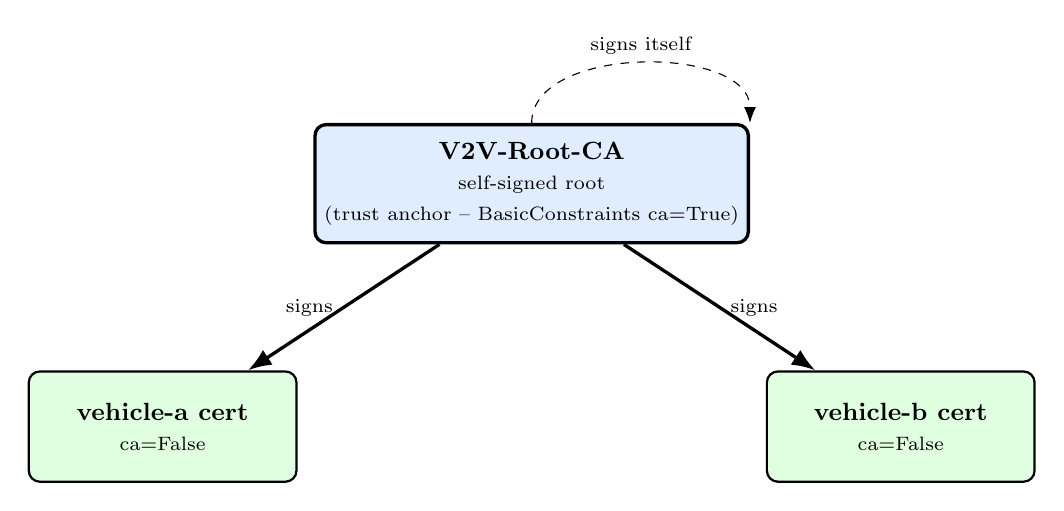
\begin{tikzpicture}[font=\small,node distance=12mm,
   ca/.style={draw,very thick,rounded corners,fill=boxblue,minimum width=4.6cm,
              minimum height=1.5cm,align=center},
   veh/.style={draw,thick,rounded corners,fill=green!12,minimum width=3.4cm,
               minimum height=1.4cm,align=center}]
  \node[ca] (ca) {\textbf{V2V-Root-CA}\\\scriptsize self-signed root\\
                   \scriptsize (trust anchor -- BasicConstraints ca=True)};
  \node[veh,below left=16mm and 2mm of ca]  (a) {\textbf{vehicle-a cert}\\\scriptsize ca=False};
  \node[veh,below right=16mm and 2mm of ca] (b) {\textbf{vehicle-b cert}\\\scriptsize ca=False};
  \draw[-{Latex[length=3mm]},very thick] (ca) -- (a)
       node[midway,left,font=\scriptsize]{signs};
  \draw[-{Latex[length=3mm]},very thick] (ca) -- (b)
       node[midway,right,font=\scriptsize]{signs};
  \draw[-{Latex[length=2mm]},dashed] (ca.north) .. controls +(0,1) and +(0,1) .. (ca.north east)
       node[midway,above,font=\scriptsize]{signs itself};
\end{tikzpicture}
\end{center}
\noindent To trust \texttt{vehicle-a}, a verifier checks just one signature:
``did V2V-Root-CA sign this?'' Trust flows down from the root.

\subsection{Diagram 2 --- Issue then Verify}
\begin{center}
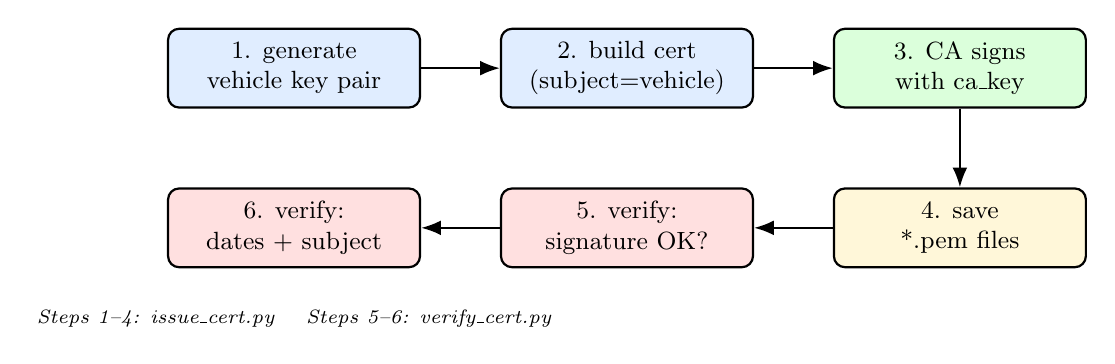
\begin{tikzpicture}[font=\small,node distance=7mm,
   box/.style={draw,thick,rounded corners,minimum width=3.2cm,minimum height=1.0cm,
               align=center}]
  \node[box,fill=boxblue]   (k)  {1. generate\\vehicle key pair};
  \node[box,fill=boxblue,right=10mm of k]   (build) {2. build cert\\(subject=vehicle)};
  \node[box,fill=green!14,right=10mm of build] (sign) {3. CA signs\\with ca\_key};
  \node[box,fill=boxyellow,below=10mm of sign] (save) {4. save\\*.pem files};
  \node[box,fill=red!12,below=10mm of build] (vsig) {5. verify:\\signature OK?};
  \node[box,fill=red!12,below=10mm of k] (vdate) {6. verify:\\dates + subject};
  \draw[-{Latex[length=2.5mm]},thick] (k) -- (build);
  \draw[-{Latex[length=2.5mm]},thick] (build) -- (sign);
  \draw[-{Latex[length=2.5mm]},thick] (sign) -- (save);
  \draw[-{Latex[length=2.5mm]},thick] (save) -- (vsig);
  \draw[-{Latex[length=2.5mm]},thick] (vsig) -- (vdate);
  \node[below=4mm of vdate,font=\scriptsize\itshape,align=left]
       {Steps 1--4: issue\_cert.py \quad Steps 5--6: verify\_cert.py};
\end{tikzpicture}
\end{center}

% =====================================================================
\section{Presentation Pack}
% =====================================================================

\subsection{Slide Outline}

\textbf{Slide 1 --- The Identity Problem.}
\begin{itemize}
  \item Two cars must trust each other before they talk.
  \item A bare public key is just a number --- it does not say \emph{whose}.
  \item We need a digital ``passport'' that cannot be faked.
  \item Solution: a Certificate Authority --- a digital passport office.
\end{itemize}

\textbf{Slide 2 --- The Certificate Authority (ca.py).}
\begin{itemize}
  \item The CA generates a P-256 key pair (\texttt{generate\_ca\_key}).
  \item It builds a \emph{self-signed} root certificate (issuer = subject).
  \item \texttt{BasicConstraints ca=True} --- it is allowed to sign others.
  \item It saves \texttt{ca\_cert.pem} (public) and \texttt{ca\_key.pem} (secret).
\end{itemize}

\textbf{Slide 3 --- Issuing a Vehicle Certificate (issue\_cert.py).}
\begin{itemize}
  \item The vehicle generates \emph{its own} key pair; the CA never sees the
        private half.
  \item The CA builds a cert with subject = vehicle, issuer = CA.
  \item \texttt{builder.sign(private\_key=ca\_key)} --- the CA's signature is the
        link in the chain of trust.
  \item Vehicle cert is \texttt{ca=False}, valid one year.
\end{itemize}

\textbf{Slide 4 --- Verifying a Certificate (verify\_cert.py).}
\begin{itemize}
  \item Three checks: signature, dates, subject.
  \item Signature check: \texttt{ca\_public\_key.verify(...)} --- the heart of it.
  \item A forged or edited certificate raises \texttt{InvalidSignature}.
  \item All three must pass $\to$ \texttt{CERTIFICATE IS VALID}.
\end{itemize}

\textbf{Slide 5 --- Why This Beats a Forged-Certificate MITM.}
\begin{itemize}
  \item Attacker has no CA private key, so cannot make a cert that verifies.
  \item Self-signed forgery $\to$ wrong signer $\to$ rejected.
  \item Edited real cert $\to$ body bytes changed $\to$ rejected.
  \item S2 (identity) + S4 (prove you own the key) together defeat MITM.
\end{itemize}

\subsection{Speaker Talking Points (about 30--60 seconds each)}

\textbf{Slide 1.} ``Before our two cars can have a secure conversation, each one
has to know it is really talking to a genuine vehicle and not an impostor. The
problem is that a public key on its own is just a long number --- it carries no
name. So we need something like a passport: a document that ties a key to an
identity and that nobody can forge. To create and check those passports we build
a Certificate Authority --- think of it as a digital passport office that
everyone agrees to trust.''

\textbf{Slide 2.} ``The file ca.py builds that authority. First it generates a
key pair on the P-256 elliptic curve --- a private key it keeps secret and a
public key it will share. Then it builds its own certificate. Because nobody
ranks above the CA, it signs that certificate with its own key --- that is what
`self-signed' means, and you can see it in the code where subject and issuer are
the same name. It marks the certificate `ca equals true', meaning this key is
allowed to sign other certificates, and saves two files: the public ca\_cert.pem,
which every vehicle gets a copy of, and the secret ca\_key.pem.''

\textbf{Slide 3.} ``Issuing a vehicle certificate is the job of issue\_cert.py.
An important detail: the vehicle generates its \emph{own} key pair --- the CA
never sees the vehicle's private key. The CA only takes the vehicle's public key,
wraps it in a certificate that names the vehicle as subject and the CA as issuer,
and then signs it with the CA's private key. That one signing line is the entire
purpose of a CA --- it is the link in the chain of trust. The vehicle certificate
is marked `ca equals false', so a vehicle can never issue certificates itself,
and it lasts one year instead of ten.''

\textbf{Slide 4.} ``verify\_cert.py is the border guard. It runs three checks.
The date check makes sure the certificate has not expired. The subject check
reads out who it belongs to. But the real test is the signature check: it takes
the CA's public key and asks `did the matching CA private key sign this exact
certificate body?'. If yes, it passes silently. If the certificate was forged or
even slightly edited, the library raises an InvalidSignature error and we reject
it. Only if all three checks pass do we print CERTIFICATE IS VALID.''

\textbf{Slide 5.} ``Here is why this defeats a man-in-the-middle who tries a fake
certificate. To make a certificate that passes our signature check, the attacker
would need the CA's private key --- and that key never leaves the CA. If they
self-sign a fake, it was signed by the wrong key and is rejected. If they edit a
real certificate, the body bytes change and the old signature no longer matches,
so it is rejected too. Section S2 proves \emph{identity}; Section S4 then makes
the vehicle prove it actually \emph{owns} the private key. Together they shut the
door on man-in-the-middle.''

\subsection{Live-Demo Script}
\begin{enumerate}
  \item \textbf{Build the CA.} Run \texttt{python ca\textbackslash ca.py}. Point
        at the line where Subject equals Issuer and say ``this is self-signed.''
  \item \textbf{Issue two certificates.} Run the two
        \texttt{issue\_cert.py} commands. Point at ``Certificate signed by CA''
        and at the SHA-256 fingerprint.
  \item \textbf{Verify a good certificate.} Run \texttt{verify\_cert.py} on
        \texttt{vehicle-a}. Point at the three \texttt{[OK]} lines and
        \texttt{CERTIFICATE IS VALID}.
  \item \textbf{Break it live.} Open \texttt{vehicle-a\_cert.pem}, change one
        Base64 character, save, re-run verify. Point at
        \texttt{[FAIL] Signature invalid} --- ``this is what happens to every
        forgery.'' Then re-issue the certificate to restore it.
\end{enumerate}

\subsection{Examiner Q\&A}
\begin{enumerate}
  \item \textbf{Q: What is a Certificate Authority?}\\
        A: A trusted party that issues and signs certificates --- a digital
        passport office. In this project it is created by \texttt{ca.py} and is
        named \texttt{V2V-Root-CA}.
  \item \textbf{Q: What does ``self-signed'' mean and why is the root self-signed?}\\
        A: The certificate's issuer and subject are the same, and it is signed
        with its own private key. The root is self-signed because nothing ranks
        above it; trust in the root must be established out-of-band by
        distributing \texttt{ca\_cert.pem}.
  \item \textbf{Q: Does the CA ever see a vehicle's private key?}\\
        A: No. The vehicle generates its own key pair in
        \texttt{generate\_vehicle\_key}; only the \emph{public} key is sent to
        the CA to be placed in the certificate and signed.
  \item \textbf{Q: How does \texttt{verify\_cert.py} detect a forged certificate?}\\
        A: \texttt{check\_signature} calls \texttt{ca\_public\_key.verify} over
        \texttt{tbs\_certificate\_bytes}. A forgery was not signed by the CA's
        private key, so verification raises \texttt{InvalidSignature}.
  \item \textbf{Q: What are \texttt{tbs\_certificate\_bytes}?}\\
        A: ``To Be Signed'' --- the exact certificate body bytes that the
        signature covers (everything except the signature itself). Verifying
        re-hashes these bytes and checks them against the signature.
  \item \textbf{Q: What do BasicConstraints and KeyUsage do?}\\
        A: BasicConstraints \texttt{ca=True/False} says whether the certificate
        may sign other certificates. KeyUsage limits the key's job ---
        \texttt{key\_cert\_sign} for the CA, \texttt{digital\_signature} for a
        vehicle. Marked critical, so a verifier must honour them.
  \item \textbf{Q: What is PEM and how does it differ from DER?}\\
        A: DER is the raw binary encoding; PEM is that binary Base64-encoded as
        text and wrapped in BEGIN/END lines so it survives copy-paste and email.
  \item \textbf{Q: Name one realistic weakness of this CA design.}\\
        A: \texttt{ca\_key.pem} is stored unencrypted (\texttt{NoEncryption()}),
        so anyone who reads that file controls the whole PKI. A real CA encrypts
        the key or keeps it in a Hardware Security Module. Also there is no
        revocation (no CRL/OCSP) --- a compromised vehicle certificate cannot be
        cancelled before it expires.
\end{enumerate}

% =====================================================================
\section{Glossary}
% =====================================================================
\begin{description}[style=nextline,leftmargin=0pt]
  \item[PKI] Public Key Infrastructure: the system of CAs, certificates and
        rules that lets strangers trust public keys.
  \item[CA] Certificate Authority: the trusted issuer and signer of certificates.
  \item[Certificate (X.509)] A standard digital document binding an identity to
        a public key, signed by an issuer.
  \item[Symmetric cryptography] One shared secret key for both locking and unlocking.
  \item[Asymmetric / public-key cryptography] A key pair: a private key kept
        secret and a public key shared freely.
  \item[Private key] The secret half of a key pair; used to sign.
  \item[Public key] The shareable half of a key pair; used to verify.
  \item[ECC] Elliptic-Curve Cryptography: public-key crypto based on curve maths.
  \item[P-256 / SECP256R1] The specific NIST elliptic curve used in this project.
  \item[SHA-256] A hash function producing a 256-bit fixed-size fingerprint.
  \item[Hash function] A one-way function turning any data into a short fingerprint.
  \item[Digital signature] A value made with a private key and checkable with the
        public key, proving authorship and integrity.
  \item[ECDSA] Elliptic Curve Digital Signature Algorithm.
  \item[Self-signed] A certificate whose issuer and subject are the same; signed
        with its own key.
  \item[Chain of trust] The line of signatures from a certificate back to a
        trusted root.
  \item[Trust anchor / root] The already-trusted certificate at the top of a chain.
  \item[Subject] Who a certificate is about.
  \item[Issuer] Who signed a certificate.
  \item[Serial number] A unique number identifying a certificate.
  \item[Fingerprint] A SHA-256 hash of a whole finished certificate, for human comparison.
  \item[BasicConstraints] Extension stating whether a certificate is a CA.
  \item[KeyUsage] Extension stating what a key is allowed to do.
  \item[Critical extension] An extension a verifier must understand or reject the cert.
  \item[Validity period] The not-before / not-after dates of a certificate.
  \item[DER] The compact binary encoding of a certificate or key.
  \item[Base64] A text encoding of binary data using 64 printable characters.
  \item[PEM] A text format: Base64 wrapped in BEGIN/END header lines.
  \item[tbs\_certificate\_bytes] The ``to-be-signed'' body bytes a signature covers.
  \item[HSM] Hardware Security Module: tamper-proof hardware for storing keys.
  \item[CRL / OCSP] Mechanisms for revoking (cancelling) a certificate early ---
        not implemented in this project.
\end{description}

% =====================================================================
\section{References and Further Study}
% =====================================================================
\begin{itemize}
  \item \textbf{Public Key Infrastructure (Wikipedia)} ---
        \url{https://en.wikipedia.org/wiki/Public_key_infrastructure}\\
        Read for: the big picture of CAs, certificates and trust.
  \item \textbf{X.509 (Wikipedia)} ---
        \url{https://en.wikipedia.org/wiki/X.509}\\
        Read for: the certificate format, fields and extensions.
  \item \textbf{RFC 5280 --- Internet X.509 Certificate Profile} ---
        \url{https://datatracker.ietf.org/doc/html/rfc5280}\\
        Read for: the authoritative definition of X.509 certificates and
        BasicConstraints / KeyUsage.
  \item \textbf{Public-key cryptography (Wikipedia)} ---
        \url{https://en.wikipedia.org/wiki/Public-key_cryptography}\\
        Read for: how key pairs work and why public keys are safe to share.
  \item \textbf{Elliptic-curve cryptography (Wikipedia)} ---
        \url{https://en.wikipedia.org/wiki/Elliptic-curve_cryptography}\\
        Read for: a gentle introduction to ECC.
  \item \textbf{ECDSA (Wikipedia)} ---
        \url{https://en.wikipedia.org/wiki/Elliptic_Curve_Digital_Signature_Algorithm}\\
        Read for: how elliptic-curve signatures sign and verify.
  \item \textbf{NIST FIPS 186-5 --- Digital Signature Standard} ---
        \url{https://csrc.nist.gov/pubs/fips/186-5/final}\\
        Read for: the official standard behind ECDSA and the P-256 curve.
  \item \textbf{SHA-2 / SHA-256 (Wikipedia)} ---
        \url{https://en.wikipedia.org/wiki/SHA-2}\\
        Read for: how the hash function used in signing works.
  \item \textbf{PEM / DER explained (Python cryptography docs)} ---
        \url{https://cryptography.io/en/latest/x509/}\\
        Read for: how this project's exact library handles certificates and PEM.
  \item \textbf{Python cryptography --- X.509 reference} ---
        \url{https://cryptography.io/en/latest/x509/reference/}\\
        Read for: \texttt{CertificateBuilder}, \texttt{load\_pem\_x509\_certificate},
        and every API used in S2.
  \item \textbf{Computerphile --- ``Public Key Cryptography'' (video)} ---
        \url{https://www.youtube.com/watch?v=GSIDS_lvRv4}\\
        Read/watch for: an intuitive, visual explanation of key pairs.
\end{itemize}

\vfill
\begin{center}\footnotesize\itshape
End of Section S2. Next: S3 --- the Cryptographic Core (AES-GCM, ECDH, HKDF, ECDSA).
\end{center}



% ===================== 03-cryptographic-core.tex =====================
\chapter{S3 --- The Cryptographic Core}

\section{Title and ``What You'll Learn''}
% =====================================================================

\subsection*{Section Title}
\textbf{S3 --- The Cryptographic Core: the toolbox of encryption, key exchange,
key derivation and signing that the rest of the project is built from.}

\subsection*{Plain-English Summary (read this first)}
Section~S3 is a single file, \texttt{crypto/crypto.py}, that contains no
networking and no protocol logic --- it is purely a \emph{toolbox} of
cryptographic functions. Four tools live here: \textbf{AES-256-GCM} locks a
message in a tamper-evident box; \textbf{ECDH} lets two cars agree on a shared
secret without ever sending it; \textbf{HKDF} turns that raw secret into a clean,
usable key; and \textbf{ECDSA} stamps a message with an unforgeable signature.
Every later section --- the handshake (S4), the secure messaging (S5) --- simply
calls these functions. Understand this file and the cryptography of the whole
project is in your hands.

\subsection*{Learning Outcomes}
After studying this section you will be able to:
\begin{itemize}
  \item Explain \textbf{symmetric encryption} and what \textbf{AES} is.
  \item Explain \textbf{authenticated encryption} and why \textbf{AES-256-GCM}
        gives confidentiality \emph{and} integrity at once.
  \item Explain the role of the \textbf{nonce} and the \textbf{authentication
        tag}.
  \item Explain \textbf{ECDH} key exchange and the Diffie--Hellman idea.
  \item Explain \textbf{HKDF} key derivation and why a raw shared secret is not
        used directly as a key.
  \item Explain \textbf{ECDSA} signing and verifying.
  \item Walk through every function in \texttt{crypto.py}, naming each argument,
        return value and exception.
  \item Run the built-in five-test demonstration and explain every output line.
  \item Explain how AES-GCM defeats the tamper attack.
\end{itemize}

% =====================================================================
\section{Where This Fits}
% =====================================================================

S3 sits \emph{underneath} Stage~2 of the pipeline. It is the engine room. The
handshake in S4 (\texttt{auth\_protocol.py}) imports seven functions directly
from \texttt{crypto.py}; the secure-messaging code in S5 uses the AES-GCM and
ECDSA functions for every BSM. S3 itself produces nothing visible --- it is the
shared library that makes Stages~2 and~3 possible.

\begin{center}
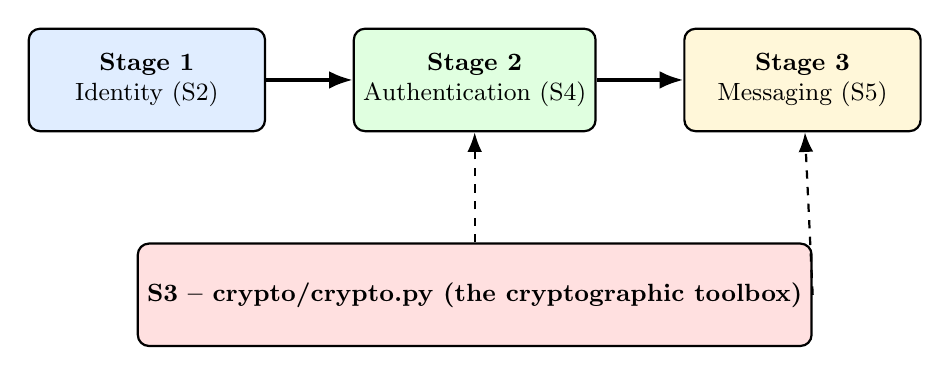
\begin{tikzpicture}[node distance=8mm and 11mm,every node/.style={font=\small},
    stage/.style={draw,rounded corners,minimum width=3.0cm,minimum height=1.3cm,
                  align=center,thick}]
  \node[stage,fill=boxblue]   (id)   {\textbf{Stage 1}\\Identity (S2)};
  \node[stage,fill=green!12,right=of id]   (auth) {\textbf{Stage 2}\\Authentication (S4)};
  \node[stage,fill=boxyellow,right=of auth] (msg) {\textbf{Stage 3}\\Messaging (S5)};
  \node[stage,fill=red!12,below=14mm of auth,minimum width=8.5cm] (core)
       {\textbf{S3 -- crypto/crypto.py (the cryptographic toolbox)}};
  \draw[-{Latex[length=3mm]},very thick] (id)   -- (auth);
  \draw[-{Latex[length=3mm]},very thick] (auth) -- (msg);
  \draw[-{Latex[length=2.5mm]},thick,dashed] (core) -- (auth);
  \draw[-{Latex[length=2.5mm]},thick,dashed] (core.east) -- (msg);
  \node[right=2mm of core.south east,font=\scriptsize\itshape] {};
\end{tikzpicture}
\end{center}

% =====================================================================
\section{The Theory You Must Study}
% =====================================================================

\subsection{Symmetric Encryption and AES}
\textbf{Plain definition.} \emph{Symmetric encryption} scrambles a message
(\emph{plaintext}) into unreadable \emph{ciphertext} using a secret key, and the
\emph{same} key unscrambles it. \textbf{AES} (Advanced Encryption Standard) is
the worldwide-standard symmetric cipher. ``AES-256'' means the key is 256 bits
(32 bytes) long.

\textbf{Real-life analogy.} A lockbox with one key. Whoever holds the key can
both lock things in and unlock them. The box without the key is just an opaque
brick --- you cannot see what is inside.

\textbf{Why it exists.} Symmetric encryption is \emph{fast} --- fast enough to
encrypt every safety message a car sends. (Public-key crypto, by contrast, is
slow; that is why it is used only for the handshake, not for every BSM.)

\textbf{How it works here.} The project uses AES with a 256-bit key
(\texttt{AES\_KEY\_LENGTH = 32}). The key itself comes from the handshake (S4).
The function \texttt{aes\_gcm\_encrypt} enforces the size: ``key must be exactly
32 bytes''.

\textbf{Security property it provides.} \textbf{Confidentiality}.

\subsection{Authenticated Encryption and AES-256-GCM}
\textbf{Plain definition.} \emph{Authenticated encryption} does two jobs in one
operation: it hides the message (confidentiality) \emph{and} produces a small
checksum-like value that detects any change (integrity). \textbf{GCM}
(Galois/Counter Mode) is the ``mode'' that adds the integrity job to AES.

\textbf{Real-life analogy.} Tamper-evident packaging on medicine. The box hides
the pills (confidentiality) \emph{and} carries a seal that visibly breaks if
anyone opened it (integrity). You get both protections from one package.

\textbf{Why it exists.} Plain encryption hides content but does \emph{not} stop
an attacker from flipping bits in the ciphertext. The receiver would happily
decrypt the corrupted message. GCM closes this hole by refusing to decrypt if
the message was changed.

\textbf{How it works here.} \texttt{aes\_gcm\_encrypt} returns three things:
\begin{itemize}
  \item the \textbf{ciphertext} --- the scrambled message;
  \item the \textbf{nonce} --- a 12-byte one-time value;
  \item the \textbf{authentication tag} --- a 16-byte (128-bit) ``seal''
        computed over the whole ciphertext.
\end{itemize}
On decryption, GCM recomputes the tag and compares. If even one bit changed, the
tags differ and the library raises \texttt{InvalidTag} --- the code turns this
into a \texttt{DecryptionError}.

\textbf{Security property it provides.} \textbf{Confidentiality} and
\textbf{integrity} together. AES-256-GCM is the same authenticated cipher used
by TLS~1.3.

\subsection{The Nonce}
\textbf{Plain definition.} A \emph{nonce} (``number used once'') is a value used
exactly once with a given key. AES-GCM needs a fresh 12-byte nonce for every
single encryption.

\textbf{Real-life analogy.} A single-use serial number on every parcel. Two
parcels must never carry the same number.

\textbf{Why it exists.} If you encrypt two different messages with the \emph{same}
key \emph{and} the same nonce, AES-GCM's security collapses --- an attacker can
learn relationships between the messages and even forge the tag. The nonce makes
each encryption unique.

\textbf{How it works here.} \texttt{aes\_gcm\_encrypt} calls
\texttt{os.urandom(12)} --- 12 cryptographically random bytes --- for every
message. With 96 random bits the chance of an accidental repeat is negligible.
The nonce is \emph{not} secret; it is sent alongside the ciphertext because the
receiver needs it to decrypt.

\textbf{Security property it provides.} It \emph{protects} confidentiality and
integrity by keeping every encryption unique.

\subsection{ECDH --- Elliptic-Curve Diffie--Hellman Key Exchange}
\textbf{Plain definition.} ECDH is a method by which two parties, each with their
own key pair, can compute the \emph{same} shared secret number --- and an
eavesdropper who sees both public keys still cannot compute it.

\textbf{Real-life analogy (the paint analogy).} Alice and Bob each start with a
secret paint colour. They mix their secret into a public colour and swap the
mixtures in the open. Each then mixes their own secret into the mixture they
received. Both end up with the identical final colour --- yet an eavesdropper who
saw only the swapped mixtures cannot un-mix them to find it.

\textbf{Why it exists.} It solves the key-distribution problem: two cars that
have never met can agree on a secret AES key over a channel the attacker is
watching, \emph{without ever transmitting the key}.

\textbf{How it works here (the mathematics, gently).} On the P-256 curve there is
a fixed public point $G$. A private key is a secret number $a$; the matching
public key is the point $a\cdot G$ (computed by ``hopping'' $G$ along the curve
$a$ times). The shared-secret magic is:
\[
a\cdot(b\cdot G)\;=\;ab\cdot G\;=\;b\cdot(a\cdot G).
\]
Vehicle~A computes $a\cdot(B\text{'s public})$; Vehicle~B computes
$b\cdot(A\text{'s public})$; both get $ab\cdot G$. An attacker sees $a\cdot G$
and $b\cdot G$ but cannot recover $a$ or $b$ (the ``elliptic-curve discrete
logarithm problem'' is infeasible). In code this is one line:
\texttt{my\_private\_key.exchange(ec.ECDH(), peer\_public\_key)}.

\textbf{Security property it provides.} It is the basis of
\textbf{confidentiality} and, because the project uses \emph{fresh} ECDH keys
each session, of \textbf{forward secrecy}.

\subsection{Ephemeral Keys and Forward Secrecy}
\textbf{Plain definition.} An \emph{ephemeral} key is generated fresh for one
session and thrown away afterwards. \textbf{Forward secrecy} is the guarantee
that recording today's encrypted traffic and stealing a key \emph{tomorrow} does
not let the attacker decrypt today's traffic.

\textbf{Real-life analogy.} A self-destructing one-time code. Even if someone
later finds your code notebook, today's code is already gone, so today's messages
stay locked forever.

\textbf{How it works here.} \texttt{generate\_ecdh\_keypair} creates a brand-new
P-256 key pair every time it is called, and the handshake calls it once per
session. The comment in the code says it plainly: ``even if an old key leaks
later, past sessions can't be decrypted because this key no longer exists.''

\textbf{Security property it provides.} \textbf{Forward secrecy}.

\subsection{HKDF --- Turning a Raw Secret into a Real Key}
\textbf{Plain definition.} HKDF (HMAC-based Key Derivation Function) is a
function that takes a rough, possibly non-uniform secret and produces a clean,
fixed-length, uniformly random key.

\textbf{Real-life analogy.} The raw ECDH output is like muddy river water ---
there is good water in it, but it is not fit to drink as-is. HKDF is the
filtration plant: in goes the rough secret, out comes clean, drinkable,
standard-sized water (a 32-byte AES key).

\textbf{Why it exists.} The raw number ECDH produces is secret, but its bits are
\emph{not} perfectly uniform, and you often want a key of an exact size. Feeding
the raw secret straight into AES is poor practice. HKDF fixes both issues. It
also lets you mix in extra public data so the final key is unique to this
session.

\textbf{How it works here.} \texttt{derive\_session\_key} calls HKDF with:
\begin{itemize}
  \item \texttt{algorithm = SHA256} --- the hash HKDF is built on;
  \item \texttt{length = 32} --- produce exactly a 32-byte AES-256 key;
  \item \texttt{salt = nonce\_a + nonce\_b} --- the two handshake nonces joined,
        making the key unique to this session;
  \item \texttt{info = b"v2v-session-key-v1"} --- a label tying the key to this
        exact purpose.
\end{itemize}
The same raw secret plus the same two nonces always yields the same 32-byte key
--- which is why both vehicles end up with an identical session key.

\textbf{Security property it provides.} It strengthens \textbf{confidentiality}
by producing a sound key, and ties the key to this session.

\subsection{SHA-256 Hashing}
\textbf{Plain definition.} A hash function turns any input into a short,
fixed-size fingerprint (SHA-256 $\to$ 256 bits). Same input, same fingerprint;
any change, completely different fingerprint; you cannot run it backwards.

\textbf{Why it exists here.} Two of S3's tools rely on it: HKDF is built on
SHA-256, and ECDSA signs the SHA-256 hash of the message rather than the whole
message.

\textbf{Security property it provides.} Supports \textbf{integrity}.

\subsection{ECDSA --- Digital Signatures}
\textbf{Plain definition.} ECDSA produces a signature with a \emph{private} key
that anyone with the matching \emph{public} key can verify. It proves \emph{who}
created the message and that it has \emph{not changed}.

\textbf{Real-life analogy.} A handwritten signature that is impossible to forge
and that also changes if the document is edited --- so the signature both
identifies the author and protects the text.

\textbf{Why it exists.} Encryption hides a message but does not prove who sent
it. A signature proves authorship, so the sender cannot later deny it.

\textbf{How it works here.} \texttt{ecdsa\_sign} calls
\texttt{private\_key.sign(message, ec.ECDSA(SHA256()))}; \texttt{ecdsa\_verify}
calls \texttt{public\_key.verify(signature, message, ec.ECDSA(SHA256()))}. The
signature is returned in \textbf{DER} encoding --- a compact standard binary
format.

\textbf{Security property it provides.} \textbf{Authentication},
\textbf{integrity}, \textbf{non-repudiation}.

\subsection{PEM Serialization of Keys}
\textbf{Plain definition.} \emph{Serialization} means turning a key object in
memory into bytes that can be saved or sent; \emph{loading} is the reverse. PEM
is the text format (Base64 between BEGIN/END lines) used.

\textbf{Why it exists here.} During the handshake a vehicle must \emph{send} its
ephemeral ECDH public key to the other vehicle. You cannot send a Python object
over a network --- you send bytes. \texttt{serialize\_public\_key} produces those
bytes; \texttt{load\_public\_key} rebuilds the key object on the other side.

\textbf{Security property it provides.} None directly --- it is about
\emph{format}. (A public key is meant to be shared, so there is nothing secret to
protect here.)

% =====================================================================
\section{Code Walkthrough}
% =====================================================================

\texttt{crypto/crypto.py} is organised as: three custom exceptions, a tiny
type-checking helper, then the four tool groups (AES-GCM, ECDH+HKDF, ECDSA, PEM),
then a built-in demonstration.

\subsection{The custom exceptions and the type guard}
\begin{lstlisting}[style=py,caption={crypto.py --- custom exceptions and the bytes guard.}]
class CryptoError(Exception):
    """Base exception for cryptographic errors in this simulation."""

class DecryptionError(CryptoError):
    """Raised when AES-GCM authentication fails during decryption."""

class SignatureError(CryptoError):
    """Raised when signature-related operations fail."""

def _ensure_bytes(value: bytes, name: str) -> None:
    if not isinstance(value, bytes):
        raise TypeError(f"{name} must be bytes")
\end{lstlisting}
\textbf{Explanation:}
\begin{enumerate}
  \item \texttt{CryptoError} is the \emph{parent} of all crypto errors, so other
        code can catch every crypto problem with one \texttt{except}.
  \item \texttt{DecryptionError} specifically means ``the message failed its
        integrity check'' --- i.e.\ possible tampering.
  \item \texttt{SignatureError} means a signing operation failed.
  \item \texttt{\_ensure\_bytes} is a small helper: cryptographic functions must
        be given raw \texttt{bytes}, not text strings. The leading underscore is
        a Python convention meaning ``private --- internal use only''.
\end{enumerate}

\subsection{aes\_gcm\_encrypt() --- lock a message}
\textbf{Purpose:} encrypt a message with AES-256-GCM, returning ciphertext, nonce
and tag.
\begin{lstlisting}[style=py,caption={crypto.py --- AES-256-GCM encryption.}]
def aes_gcm_encrypt(key: bytes, plaintext: bytes) -> tuple[bytes, bytes, bytes]:
    _ensure_bytes(key, "key")
    _ensure_bytes(plaintext, "plaintext")

    if len(key) != 32:
        raise ValueError("key must be exactly 32 bytes for AES-256-GCM")

    nonce = os.urandom(12)
    aesgcm = AESGCM(key)
    encrypted_blob = aesgcm.encrypt(nonce, plaintext, None)
    ciphertext = encrypted_blob[:-16]
    auth_tag = encrypted_blob[-16:]
    return ciphertext, nonce, auth_tag
\end{lstlisting}
\textbf{Step by step:}
\begin{enumerate}
  \item Check both arguments are \texttt{bytes}.
  \item Check the key is exactly 32 bytes --- that is what makes it AES-\emph{256}.
        A wrong size raises \texttt{ValueError}.
  \item \texttt{os.urandom(12)} draws a fresh 12-byte random nonce --- new for
        every call.
  \item \texttt{AESGCM(key)} creates the cipher object bound to that key.
  \item \texttt{aesgcm.encrypt(nonce, plaintext, None)} encrypts. The third
        argument is the \emph{associated data} (extra data to authenticate but
        not encrypt); \texttt{None} means none is used here. The library returns
        a single blob: \texttt{ciphertext} followed by the 16-byte tag.
  \item \texttt{encrypted\_blob[:-16]} is everything except the last 16 bytes ---
        the ciphertext. \texttt{encrypted\_blob[-16:]} is the last 16 bytes ---
        the authentication tag. The code splits them so callers can store them
        separately.
\end{enumerate}
\textbf{Arguments:} \texttt{key} (32 bytes), \texttt{plaintext} (bytes).
\textbf{Returns:} a 3-tuple \texttt{(ciphertext, nonce, auth\_tag)}.
\textbf{Exceptions:} \texttt{TypeError} (not bytes), \texttt{ValueError} (key not
32 bytes). \textbf{Theory link:} authenticated encryption, the nonce, the tag.
\emph{Analogy:} sealing the message in tamper-evident packaging and printing a
fresh serial number (nonce) on it.

\subsection{aes\_gcm\_decrypt() --- unlock and verify}
\textbf{Purpose:} decrypt AES-GCM ciphertext \emph{and} verify it was not
tampered with.
\begin{lstlisting}[style=py,caption={crypto.py --- AES-256-GCM decryption with tamper detection.}]
def aes_gcm_decrypt(key, ciphertext, nonce, tag) -> bytes:
    _ensure_bytes(key, "key"); _ensure_bytes(ciphertext, "ciphertext")
    _ensure_bytes(nonce, "nonce"); _ensure_bytes(tag, "tag")

    if len(key) != 32:   raise ValueError("key must be exactly 32 bytes ...")
    if len(nonce) != 12: raise ValueError("nonce must be exactly 12 bytes ...")
    if len(tag) != 16:   raise ValueError("tag must be exactly 16 bytes ...")

    encrypted_blob = ciphertext + tag
    aesgcm = AESGCM(key)
    try:
        return aesgcm.decrypt(nonce, encrypted_blob, None)
    except InvalidTag as exc:
        raise DecryptionError(
            "Message authentication failed - possible tampering detected"
        ) from exc
\end{lstlisting}
\textbf{Step by step:}
\begin{enumerate}
  \item Check all four arguments are \texttt{bytes}.
  \item Check the exact lengths: key 32, nonce 12, tag 16. Any wrong size raises
        \texttt{ValueError} --- a clear ``programmer error'' rather than a
        security event.
  \item Re-join \texttt{ciphertext + tag} into the single blob the library
        expects (the opposite of the split done during encryption).
  \item \texttt{aesgcm.decrypt(...)} does two things in one step: it decrypts and
        it re-computes the tag and compares it.
  \item If the tag matches, it returns the original plaintext. If the ciphertext,
        nonce or tag was altered, the library raises \texttt{InvalidTag}; the
        code catches it and re-raises a friendlier \texttt{DecryptionError}.
\end{enumerate}
\textbf{The crucial idea:} a tampered message does \emph{not} decrypt to garbage
--- it \emph{refuses to decrypt at all}. There is no way to ``ignore'' a bad tag.
\textbf{Theory link:} authenticated encryption providing integrity.
\emph{Analogy:} the pharmacist seeing the broken seal and refusing to hand over
the medicine.

\subsection{generate\_ecdh\_keypair() --- a fresh key pair per session}
\begin{lstlisting}[style=py,caption={crypto.py --- generate an ephemeral ECDH key pair.}]
def generate_ecdh_keypair():
    # We generate a NEW key pair each session (ephemeral).
    # This provides "Forward Secrecy".
    private_key = ec.generate_private_key(ec.SECP256R1(), default_backend())
    public_key = private_key.public_key()
    return private_key, public_key
\end{lstlisting}
\textbf{Step by step:} create a new P-256 private key; derive its public key;
return both. There are no arguments. \textbf{Returns:} a tuple
\texttt{(private\_key, public\_key)}. \textbf{Theory link:} ephemeral keys and
forward secrecy --- because it is called fresh for each session, an old key
simply does not exist any more.

\subsection{ecdh\_shared\_secret() --- compute the shared number}
\begin{lstlisting}[style=py,caption={crypto.py --- ECDH shared-secret computation.}]
def ecdh_shared_secret(my_private_key, peer_public_key) -> bytes:
    if not isinstance(my_private_key, ec.EllipticCurvePrivateKey):
        raise TypeError("my_private_key must be an EllipticCurvePrivateKey")
    if not isinstance(peer_public_key, ec.EllipticCurvePublicKey):
        raise TypeError("peer_public_key must be an EllipticCurvePublicKey")
    try:
        return my_private_key.exchange(ec.ECDH(), peer_public_key)
    except Exception as exc:
        raise CryptoError("failed to compute ECDH shared secret") from exc
\end{lstlisting}
\textbf{Step by step:}
\begin{enumerate}
  \item Confirm the first argument is a private key and the second is a public key.
  \item \texttt{my\_private\_key.exchange(ec.ECDH(), peer\_public\_key)} performs
        the elliptic-curve multiplication $a\cdot(b\cdot G)$ and returns the raw
        shared-secret bytes.
  \item Any failure is wrapped as a \texttt{CryptoError}.
\end{enumerate}
\textbf{Key fact:} if Vehicle~A calls this with (A-private, B-public) and
Vehicle~B calls it with (B-private, A-public), \emph{both get the identical
bytes}. \textbf{Returns:} the raw shared secret (bytes). \textbf{Theory link:}
ECDH key exchange. \emph{Analogy:} both painters finishing with the same final
colour.

\subsection{derive\_session\_key() --- raw secret to clean AES key}
\begin{lstlisting}[style=py,caption={crypto.py --- HKDF key derivation.}]
def derive_session_key(shared_secret, nonce_a, nonce_b) -> bytes:
    _ensure_bytes(shared_secret, "shared_secret")
    _ensure_bytes(nonce_a, "nonce_a")
    _ensure_bytes(nonce_b, "nonce_b")

    hkdf = HKDF(
        algorithm=hashes.SHA256(),
        length=32,
        salt=nonce_a + nonce_b,
        info=b"v2v-session-key-v1",
        backend=default_backend(),
    )
    return hkdf.derive(shared_secret)
\end{lstlisting}
\textbf{Step by step:}
\begin{enumerate}
  \item Check all three arguments are bytes.
  \item Build an \texttt{HKDF} object: SHA-256 as the base hash;
        \texttt{length=32} so the output is exactly an AES-256 key;
        \texttt{salt} is the two session nonces joined together;
        \texttt{info} is the fixed purpose label.
  \item \texttt{hkdf.derive(shared\_secret)} runs the raw ECDH secret through
        HKDF and returns the clean 32-byte key.
\end{enumerate}
\textbf{Why salt = nonce\_a + nonce\_b?} The raw ECDH secret could repeat if the
same ephemeral keys were ever reused; mixing in two fresh random nonces
guarantees the \emph{derived} key is unique to this session.
\textbf{Honest note:} the string \texttt{b"v2v-session-key-v1"} is written
directly here even though \texttt{config.py} already defines
\texttt{SESSION\_KEY\_INFO} with the same value --- a small duplication worth
mentioning if asked. \textbf{Returns:} a 32-byte key. \textbf{Theory link:} HKDF.
\emph{Analogy:} the filtration plant turning muddy water into clean water.

\subsection{ecdsa\_sign() and ecdsa\_verify() --- digital signatures}
\begin{lstlisting}[style=py,caption={crypto.py --- ECDSA signing and verification.}]
def ecdsa_sign(private_key, message: bytes) -> bytes:
    if not isinstance(private_key, ec.EllipticCurvePrivateKey):
        raise TypeError("private_key must be an EllipticCurvePrivateKey")
    _ensure_bytes(message, "message")
    try:
        return private_key.sign(message, ec.ECDSA(hashes.SHA256()))
    except Exception as exc:
        raise SignatureError("failed to create ECDSA signature") from exc

def ecdsa_verify(public_key, message: bytes, signature: bytes) -> bool:
    if not isinstance(public_key, ec.EllipticCurvePublicKey):
        raise TypeError("public_key must be an EllipticCurvePublicKey")
    _ensure_bytes(message, "message")
    _ensure_bytes(signature, "signature")
    try:
        public_key.verify(signature, message, ec.ECDSA(hashes.SHA256()))
        return True
    except InvalidSignature:
        return False
\end{lstlisting}
\textbf{ecdsa\_sign --- step by step:}
\begin{enumerate}
  \item Confirm the key is a private key and the message is bytes.
  \item \texttt{private\_key.sign(message, ec.ECDSA(SHA256()))} hashes the
        message with SHA-256 and signs that hash. It returns the signature in
        DER encoding.
  \item Any failure becomes a \texttt{SignatureError}.
\end{enumerate}
\textbf{ecdsa\_verify --- step by step:}
\begin{enumerate}
  \item Confirm the key is a public key and the other two arguments are bytes.
  \item \texttt{public\_key.verify(signature, message, ec.ECDSA(SHA256()))}
        re-hashes the message and checks the signature against it.
  \item If valid, \texttt{verify} returns silently and the function returns
        \texttt{True}. If invalid it raises \texttt{InvalidSignature}, which is
        caught and turned into \texttt{False}.
\end{enumerate}
\textbf{Design note:} \texttt{ecdsa\_verify} returns a plain
\texttt{True}/\texttt{False} rather than raising --- this makes it easy for the
handshake code to write \texttt{if not ecdsa\_verify(...)}. \textbf{Theory link:}
ECDSA, authentication, integrity, non-repudiation. \emph{Analogy:} pressing the
wax seal (sign) and inspecting it (verify).

\subsection{serialize\_public\_key(), load\_public\_key(), load\_private\_key()}
These three are the PEM bridge between in-memory key objects and bytes.
\begin{lstlisting}[style=py,caption={crypto.py --- PEM serialization helpers.}]
def serialize_public_key(pub_key) -> bytes:
    if not isinstance(pub_key, ec.EllipticCurvePublicKey):
        raise TypeError("pub_key must be an EllipticCurvePublicKey")
    return pub_key.public_bytes(
        encoding=serialization.Encoding.PEM,
        format=serialization.PublicFormat.SubjectPublicKeyInfo,
    )

def load_public_key(pem_data: bytes) -> ec.EllipticCurvePublicKey:
    _ensure_bytes(pem_data, "pem_data")
    try:
        public_key = serialization.load_pem_public_key(pem_data, backend=default_backend())
    except Exception as exc:
        raise ValueError("invalid PEM public key data") from exc
    if not isinstance(public_key, ec.EllipticCurvePublicKey):
        raise ValueError("loaded key is not an elliptic-curve public key")
    return public_key
\end{lstlisting}
\textbf{Explanation:}
\begin{enumerate}
  \item \texttt{serialize\_public\_key} turns a public-key object into PEM text
        bytes (so it can be put inside a handshake message and sent).
  \item \texttt{load\_public\_key} parses PEM bytes back into a key object, and
        rejects anything that is not a valid elliptic-curve public key.
  \item \texttt{load\_private\_key} (not shown, same shape) parses a PEM private
        key with \texttt{password=None}, matching the un-encrypted key files from
        S2.
\end{enumerate}
\textbf{Theory link:} PEM serialization. \emph{Analogy:} flattening a 3-D object
into a printed sheet so it can be posted, then folding it back up on arrival.

\subsection{The built-in demonstration (\texttt{if \_\_name\_\_ == "\_\_main\_\_"})}
At the bottom of the file is a five-test self-demonstration that runs only when
the file is executed directly. It is excellent for learning because it exercises
every tool: Test~1 proves ECDH gives both sides the same secret; Test~2 derives a
session key; Test~3 encrypts then decrypts a message; Test~4 signs and verifies
(and shows verification \emph{fails} with the wrong key); Test~5 flips one bit of
ciphertext and confirms the tampered message is rejected. We run it in the next
section.

% =====================================================================
\section{Hands-On / Practical}
% =====================================================================

\subsection{Run the cryptographic core by itself}
\texttt{crypto.py} needs no certificates and no network --- just run it:
\begin{lstlisting}[style=term]
python crypto\crypto.py
\end{lstlisting}

\noindent\textbf{Expected output (sample). Note: where this guide shows
\texttt{[OK]}, the real terminal prints a small check-mark character, because the
source uses the escape \texttt{\textbackslash u2713}.}
\begin{lstlisting}[style=term]
=== CRYPTO MODULE DEMONSTRATION ===

[TEST 1] ECDH Key Exchange
Vehicle A secret == Vehicle B secret: True

[TEST 2] Session Key Derivation
Session key (hex): 9f3c1a...e7b2   (64 hex characters)
Session key length: 32 bytes

[TEST 3] AES-GCM Encrypt/Decrypt
Decrypted: Hello from Vehicle A! [OK]

[TEST 4] ECDSA Sign/Verify
Signature valid with matching key: True
Signature valid with wrong key: False

[TEST 5] Tamper Detection
Tampered message correctly rejected [OK]
\end{lstlisting}

\subsection{What each output line means}
\begin{itemize}
  \item \textbf{Test 1 --- \texttt{True}}: the two vehicles, using only each
        other's \emph{public} keys, computed the \emph{same} secret. ECDH works.
  \item \textbf{Test 2 --- 32 bytes}: HKDF turned the raw secret into exactly a
        256-bit AES key. The hex string is 64 characters because each byte is two
        hex digits.
  \item \textbf{Test 3 --- ``Decrypted: Hello from Vehicle A!''}: encrypt then
        decrypt round-trips perfectly --- confidentiality with no data loss.
  \item \textbf{Test 4 --- \texttt{True} then \texttt{False}}: the signature
        verifies with the correct public key, but \emph{fails} with the wrong
        key. That ``False'' is exactly how impersonation is detected.
  \item \textbf{Test 5 --- ``rejected''}: one bit of ciphertext was flipped;
        decryption refused. That is the tamper defence working.
\end{itemize}

\subsection{Try This Yourself (mini-experiment): break the tag}
Test~5 already flips a \emph{ciphertext} bit. Try flipping the \emph{tag}
instead. Add a few lines to the demo (or open a Python shell):
\begin{lstlisting}[style=term]
ct, nc, tag = aes_gcm_encrypt(session_key, b"hello")
bad_tag = bytearray(tag)
bad_tag[0] ^= 0x01                       # flip one bit of the tag
aes_gcm_decrypt(session_key, ct, nc, bytes(bad_tag))
\end{lstlisting}
\textbf{Predict before you run.} The tag is part of what GCM checks, so a changed
tag is just as fatal as changed ciphertext. Prediction: a
\texttt{DecryptionError} (``possible tampering detected'') is raised. Lesson: the
nonce, the ciphertext \emph{and} the tag are all protected --- you cannot edit
any of them and still decrypt.

\textbf{Second experiment:} keep the ciphertext and tag correct but change the
\emph{nonce} by one bit. Predict: still a \texttt{DecryptionError}, because the
tag was computed for the original nonce.

% =====================================================================
\section{Attack Relevance}
% =====================================================================

S3 is the \emph{toolbox}, so it supplies the defence used against \emph{three}
of the four attacks. The defences are exercised directly by
\texttt{attacks/tamper\_attack.py}.

\begin{table}[h]
\centering
\small
\begin{tabular}{@{}p{2.6cm} p{6.0cm} p{4.9cm}@{}}
\toprule
\textbf{Attack} & \textbf{How an S3 tool stops it} & \textbf{The function}\\
\midrule
Tamper & Any change to ciphertext, nonce or tag makes the GCM tag mismatch;
decryption refuses. & \texttt{aes\_gcm\_decrypt} (raises \texttt{DecryptionError}).\\
Eavesdrop & The message is AES-256 ciphertext; without the session key it is
unreadable noise. & \texttt{aes\_gcm\_encrypt}.\\
Impersonation & A forged message will not carry a signature that verifies under
the real vehicle's public key. & \texttt{ecdsa\_verify} (returns \texttt{False}).\\
\bottomrule
\end{tabular}
\caption{Which S3 tool defends against which attack.}
\end{table}

\noindent\textbf{The tamper attack in detail.} The attacker captures an encrypted
BSM and flips bits hoping to change ``speed 80'' into something dangerous. But
the AES-GCM tag is computed over the \emph{whole} ciphertext. The receiver's call
to \texttt{aes\_gcm\_decrypt} re-computes the tag, sees a mismatch, and raises
\texttt{DecryptionError} instead of returning data. The attacker cannot fix the
tag because they do not have the session key. \textbf{Forward secrecy} is also an
S3 contribution: \texttt{generate\_ecdh\_keypair} makes a throw-away key each
session, so a key stolen later cannot decrypt recorded traffic.

\textbf{Honest scope note.} S3 provides the \emph{primitives}; it does not by
itself decide \emph{when} to use them or check timestamps and nonces --- that
sequencing is the protocol logic in S4 and S5. A primitive used incorrectly (for
example, reusing a nonce) would still be insecure; S3 just makes correct use
possible.

% =====================================================================
\section{Illustrations}
% =====================================================================

\subsection{Diagram 1 --- AES-256-GCM Encrypt then Decrypt}
\begin{center}
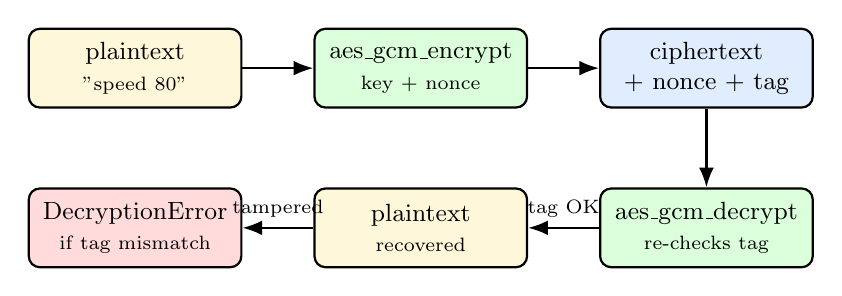
\begin{tikzpicture}[font=\small,node distance=6mm,
   box/.style={draw,thick,rounded corners,minimum width=2.7cm,minimum height=1.0cm,
               align=center}]
  \node[box,fill=boxyellow] (pt) {plaintext\\\scriptsize "speed 80"};
  \node[box,fill=green!14,right=9mm of pt] (enc) {aes\_gcm\_encrypt\\\scriptsize key + nonce};
  \node[box,fill=boxblue,right=9mm of enc] (out) {ciphertext\\+ nonce + tag};
  \node[box,fill=green!14,below=10mm of out] (dec) {aes\_gcm\_decrypt\\\scriptsize re-checks tag};
  \node[box,fill=boxyellow,left=9mm of dec] (pt2) {plaintext\\\scriptsize recovered};
  \node[box,fill=red!14,left=9mm of pt2] (fail) {DecryptionError\\\scriptsize if tag mismatch};
  \draw[-{Latex[length=2.5mm]},thick] (pt) -- (enc);
  \draw[-{Latex[length=2.5mm]},thick] (enc) -- (out);
  \draw[-{Latex[length=2.5mm]},thick] (out) -- (dec);
  \draw[-{Latex[length=2.5mm]},thick] (dec) -- (pt2) node[midway,above,font=\scriptsize]{tag OK};
  \draw[-{Latex[length=2.5mm]},thick] (pt2) -- (fail) node[midway,above,font=\scriptsize]{tampered};
\end{tikzpicture}
\end{center}

\subsection{Diagram 2 --- ECDH gives both sides the same secret}
\begin{center}
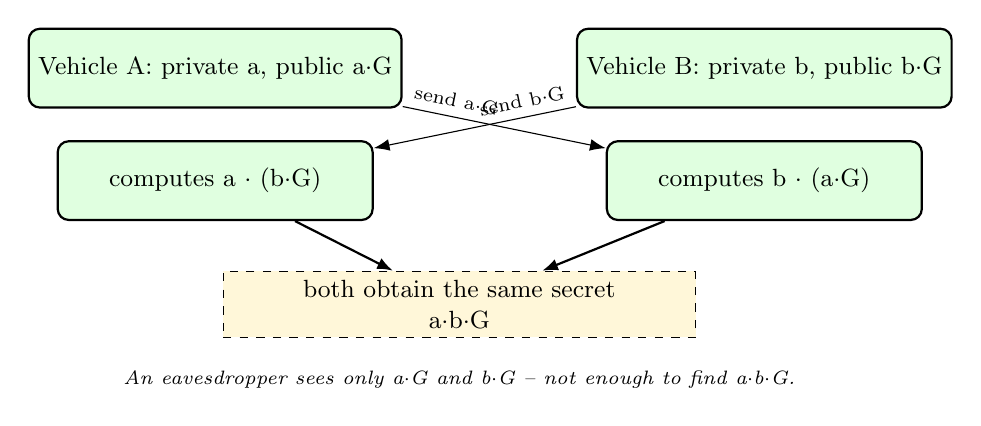
\begin{tikzpicture}[font=\small,node distance=5mm,
   v/.style={draw,thick,rounded corners,fill=green!12,minimum width=4.0cm,
             minimum height=1.0cm,align=center}]
  \node[v] (a1) {Vehicle A: private a, public a$\cdot$G};
  \node[v,below=4mm of a1] (a2) {computes a $\cdot$ (b$\cdot$G)};
  \node[v,right=22mm of a1] (b1) {Vehicle B: private b, public b$\cdot$G};
  \node[v,below=4mm of b1] (b2) {computes b $\cdot$ (a$\cdot$G)};
  \node[draw,dashed,fill=boxyellow,minimum width=6cm,align=center] (s)
       at (3.1,-3.0)
       {both obtain the same secret\\ a$\cdot$b$\cdot$G};
  \draw[-{Latex[length=2mm]}] (a1) -- (b2)
       node[pos=0.25,above,font=\scriptsize,sloped]{send a$\cdot$G};
  \draw[-{Latex[length=2mm]}] (b1) -- (a2)
       node[pos=0.25,above,font=\scriptsize,sloped]{send b$\cdot$G};
  \draw[-{Latex[length=2mm]},thick] (a2) -- (s);
  \draw[-{Latex[length=2mm]},thick] (b2) -- (s);
  \node[below=3mm of s,font=\scriptsize\itshape]
       {An eavesdropper sees only a$\cdot$G and b$\cdot$G -- not enough to find a$\cdot$b$\cdot$G.};
\end{tikzpicture}
\end{center}

\subsection{Diagram 3 --- The S3 pipeline that builds a session key}
\begin{center}
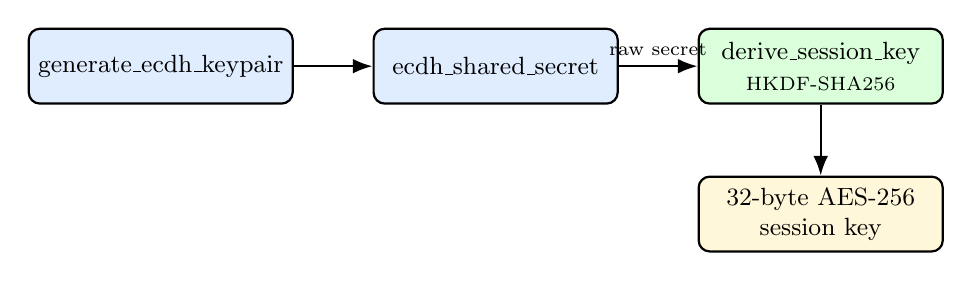
\begin{tikzpicture}[font=\small,node distance=8mm,
   box/.style={draw,thick,rounded corners,minimum width=3.1cm,minimum height=0.95cm,
               align=center}]
  \node[box,fill=boxblue] (kp) {generate\_ecdh\_keypair};
  \node[box,fill=boxblue,right=10mm of kp] (ss) {ecdh\_shared\_secret};
  \node[box,fill=green!14,right=10mm of ss] (dk) {derive\_session\_key\\\scriptsize HKDF-SHA256};
  \node[box,fill=boxyellow,below=9mm of dk] (key) {32-byte AES-256\\session key};
  \draw[-{Latex[length=2.5mm]},thick] (kp) -- (ss);
  \draw[-{Latex[length=2.5mm]},thick] (ss) -- (dk) node[midway,above,font=\scriptsize]{raw secret};
  \draw[-{Latex[length=2.5mm]},thick] (dk) -- (key);
\end{tikzpicture}
\end{center}

% =====================================================================
\section{Presentation Pack}
% =====================================================================

\subsection{Slide Outline}

\textbf{Slide 1 --- The Crypto Toolbox.}
\begin{itemize}
  \item \texttt{crypto.py} is a library, not a program --- four tools.
  \item AES-256-GCM: lock + tamper seal. ECDH: agree a secret. HKDF: clean the
        secret. ECDSA: sign.
  \item Every later section calls these functions.
  \item Industry-standard --- the same set used by TLS 1.3.
\end{itemize}

\textbf{Slide 2 --- AES-256-GCM: Authenticated Encryption.}
\begin{itemize}
  \item Encrypt returns three things: ciphertext, nonce, 16-byte tag.
  \item The tag is a seal over the whole ciphertext.
  \item Decrypt re-checks the tag; one changed bit $\to$ \texttt{DecryptionError}.
  \item Gives confidentiality AND integrity in one step.
\end{itemize}

\textbf{Slide 3 --- ECDH + HKDF: Building a Shared Key.}
\begin{itemize}
  \item ECDH: two cars compute the same secret without sending it.
  \item Maths: a$\cdot$(b$\cdot$G) = b$\cdot$(a$\cdot$G).
  \item Keys are ephemeral $\to$ forward secrecy.
  \item HKDF filters the raw secret into a clean 32-byte AES key.
\end{itemize}

\textbf{Slide 4 --- ECDSA: Digital Signatures.}
\begin{itemize}
  \item Sign with the private key, verify with the public key.
  \item Proves who wrote it (authentication) and that it is unchanged (integrity).
  \item \texttt{ecdsa\_verify} returns \texttt{True}/\texttt{False}.
  \item Wrong key $\to$ \texttt{False} $\to$ impersonation detected.
\end{itemize}

\textbf{Slide 5 --- Live Proof: the Five-Test Demo.}
\begin{itemize}
  \item Test 1: ECDH secrets match. Test 2: 32-byte key derived.
  \item Test 3: encrypt/decrypt round-trips.
  \item Test 4: signature good with right key, fails with wrong key.
  \item Test 5: a flipped bit is rejected --- the tamper defence.
\end{itemize}

\subsection{Speaker Talking Points (about 30--60 seconds each)}

\textbf{Slide 1.} ``This section is one file, crypto.py, and it is unusual ---
it contains no networking and no protocol. It is purely a toolbox of four
cryptographic tools. AES-256-GCM is our lockbox with a built-in tamper seal. ECDH
lets two cars secretly agree on a key. HKDF cleans that key up. And ECDSA is our
unforgeable signature. Everything else in the project --- the handshake, the
secure messaging --- just calls these functions. And these are not toy
algorithms: this is the exact same set of building blocks used by TLS 1.3, the
security behind every HTTPS website.''

\textbf{Slide 2.} ``AES-256-GCM is authenticated encryption. When you encrypt,
you get back three things: the ciphertext, a nonce, and a 16-byte authentication
tag. Think of the tag as a wax seal stamped over the whole ciphertext. When you
decrypt, the library does not just unscramble --- it recomputes the tag and
compares. If even one bit of the ciphertext, the nonce or the tag was changed,
the tags disagree and decryption is refused; our code raises a DecryptionError.
So with one operation we get confidentiality --- the content is hidden --- and
integrity --- any change is caught.''

\textbf{Slide 3.} ``How do two cars that have never met get a shared secret key
over a channel an attacker is watching? That is ECDH. Each car has a private
number and a public point. They swap public points in the open. Then each mixes
its own private number with the other's public point. Thanks to the curve maths
--- a times b-times-G equals b times a-times-G --- both arrive at the identical
secret, while an eavesdropper who saw only the public points cannot compute it.
And because we generate a fresh ECDH key for every session and throw it away, a
key stolen tomorrow cannot unlock today's traffic --- that is forward secrecy.
Finally HKDF takes that raw secret, which is not perfectly uniform, and filters
it into a clean 32-byte AES key.''

\textbf{Slide 4.} ``ECDSA is our digital signature. You sign with your private
key; anyone can verify with your public key. A signature proves two things at
once: who created the message, and that it has not been changed since. In the
code, ecdsa\_verify simply returns True or False. And here is the security point
--- if an impostor signs a message with the wrong key, verification returns
False. That single False is how we catch impersonation.''

\textbf{Slide 5.} ``The best part is that crypto.py proves itself. Run it
directly and it executes five tests. Test one shows the two ECDH secrets are
equal. Test two shows HKDF produced a 32-byte key. Test three encrypts and
decrypts a message and recovers it exactly. Test four signs a message and shows
verification succeeds with the right key and fails with the wrong one. And test
five flips a single bit of ciphertext and shows the message is rejected. Five
tests, every tool, all visible on screen.''

\subsection{Live-Demo Script}
\begin{enumerate}
  \item \textbf{Run the toolbox.} Execute \texttt{python crypto\textbackslash
        crypto.py}. Point at \texttt{[TEST 1] ... True} --- ``both cars derived
        the same secret without sending it.''
  \item \textbf{Point at Test 2.} ``32 bytes --- that is our AES-256 key.''
  \item \textbf{Point at Test 4.} ``True with the right key, False with the
        wrong key --- that False is impersonation being caught.''
  \item \textbf{Point at Test 5.} ``One bit flipped, message rejected --- the
        tamper defence.''
  \item \textbf{Optional.} In a Python shell, flip a bit of the \emph{tag} (see
        the mini-experiment) and show the same \texttt{DecryptionError}.
\end{enumerate}

\subsection{Examiner Q\&A}
\begin{enumerate}
  \item \textbf{Q: What does the ``GCM'' in AES-256-GCM add over plain AES?}\\
        A: GCM (Galois/Counter Mode) adds \emph{authentication}: a 16-byte tag
        computed over the ciphertext. It turns AES into \emph{authenticated}
        encryption, giving integrity as well as confidentiality.
  \item \textbf{Q: Why must the nonce never repeat for the same key?}\\
        A: Reusing a (key, nonce) pair in GCM breaks security --- it can leak
        relationships between messages and allow tag forgery. The code uses a
        fresh \texttt{os.urandom(12)} nonce every time to prevent this.
  \item \textbf{Q: Is the nonce secret?}\\
        A: No. It is sent alongside the ciphertext because the receiver needs it
        to decrypt. Security depends on \emph{uniqueness}, not secrecy.
  \item \textbf{Q: How does ECDH let two cars share a key without sending it?}\\
        A: Each car combines its own private key with the other's public key.
        The curve maths makes both results equal (\,a$\cdot$b$\cdot$G\,), and an
        eavesdropper with only the public keys cannot compute it.
  \item \textbf{Q: Why use HKDF instead of using the ECDH output directly?}\\
        A: The raw ECDH secret is not perfectly uniform and may not be the right
        size. HKDF extracts and expands it into a clean, fixed-length key, and
        the nonce salt ties the key to this one session.
  \item \textbf{Q: What happens in \texttt{aes\_gcm\_decrypt} if a message is
        tampered with?}\\
        A: The recomputed tag does not match, the library raises
        \texttt{InvalidTag}, and the code re-raises it as \texttt{DecryptionError}
        --- no plaintext is ever returned.
  \item \textbf{Q: Why does \texttt{ecdsa\_verify} return a boolean instead of
        raising?}\\
        A: A failed signature is an expected, normal event during an attack, not
        a programming bug. Returning \texttt{False} lets callers write a simple
        \texttt{if not ecdsa\_verify(...)} check.
  \item \textbf{Q: This file is called a ``toolbox'' --- what does it \emph{not}
        do?}\\
        A: It provides primitives only. It does not check timestamps, manage
        nonces against replay, or sequence the handshake --- that protocol logic
        lives in S4 and S5. Correct \emph{use} of the primitives is the
        protocol's responsibility.
\end{enumerate}

% =====================================================================
\section{Glossary}
% =====================================================================
\begin{description}[style=nextline,leftmargin=0pt]
  \item[Plaintext] The original readable message before encryption.
  \item[Ciphertext] The scrambled, unreadable output of encryption.
  \item[Symmetric encryption] Encryption using one shared secret key for both directions.
  \item[AES] Advanced Encryption Standard: the worldwide-standard symmetric cipher.
  \item[AES-256] AES with a 256-bit (32-byte) key.
  \item[GCM] Galois/Counter Mode: the AES mode that adds an authentication tag.
  \item[Authenticated encryption] Encryption that also detects any tampering.
  \item[Nonce] A number used exactly once with a given key.
  \item[Authentication tag] The 16-byte value GCM computes to detect tampering.
  \item[Associated data (AAD)] Extra data authenticated but not encrypted (here: none).
  \item[ECDH] Elliptic-Curve Diffie--Hellman: a shared-secret key-exchange method.
  \item[Shared secret] The identical secret value two parties compute via ECDH.
  \item[Ephemeral key] A key generated for one session and then discarded.
  \item[Forward secrecy] Past traffic stays secret even if a key leaks later.
  \item[HKDF] HMAC-based Key Derivation Function: turns a raw secret into a clean key.
  \item[Salt] Extra input to HKDF (here the two nonces) making the key session-unique.
  \item[Info string] A label fed to HKDF binding the key to a specific purpose.
  \item[SHA-256] A hash function producing a 256-bit fingerprint.
  \item[ECDSA] Elliptic Curve Digital Signature Algorithm.
  \item[Digital signature] A private-key-made value verifiable with the public key.
  \item[DER] A compact binary encoding (used here for signatures).
  \item[PEM] A text encoding (Base64 + BEGIN/END lines) used for keys.
  \item[Serialization] Converting an in-memory object into bytes for storage/transmission.
  \item[InvalidTag] The library error raised when a GCM tag does not match.
  \item[DecryptionError] This project's exception meaning ``possible tampering''.
  \item[Session key] The 32-byte AES key used to encrypt one conversation.
\end{description}

% =====================================================================
\section{References and Further Study}
% =====================================================================
\begin{itemize}
  \item \textbf{Python cryptography --- AES-GCM (AESGCM) docs} ---
        \url{https://cryptography.io/en/latest/hazmat/primitives/aead/}\\
        Read for: the exact \texttt{AESGCM} class used in \texttt{crypto.py}.
  \item \textbf{Python cryptography --- elliptic-curve docs} ---
        \url{https://cryptography.io/en/latest/hazmat/primitives/asymmetric/ec/}\\
        Read for: ECDH \texttt{exchange()} and ECDSA \texttt{sign/verify}.
  \item \textbf{Python cryptography --- HKDF docs} ---
        \url{https://cryptography.io/en/latest/hazmat/primitives/key-derivation-functions/}\\
        Read for: the \texttt{HKDF} class, its salt and info parameters.
  \item \textbf{NIST SP 800-38D --- GCM mode of operation} ---
        \url{https://csrc.nist.gov/pubs/sp/800/38/d/final}\\
        Read for: the official definition of AES-GCM and the nonce rule.
  \item \textbf{NIST FIPS 197 --- the AES standard} ---
        \url{https://csrc.nist.gov/pubs/fips/197/final}\\
        Read for: what AES itself is.
  \item \textbf{RFC 5869 --- HKDF} ---
        \url{https://datatracker.ietf.org/doc/html/rfc5869}\\
        Read for: why extract-then-expand key derivation is done this way.
  \item \textbf{Diffie--Hellman key exchange (Wikipedia)} ---
        \url{https://en.wikipedia.org/wiki/Diffie%E2%80%93Hellman_key_exchange}\\
        Read for: the paint analogy and the original idea behind ECDH.
  \item \textbf{Authenticated encryption (Wikipedia)} ---
        \url{https://en.wikipedia.org/wiki/Authenticated_encryption}\\
        Read for: why confidentiality alone is not enough.
  \item \textbf{Galois/Counter Mode (Wikipedia)} ---
        \url{https://en.wikipedia.org/wiki/Galois/Counter_Mode}\\
        Read for: how the GCM tag is built.
  \item \textbf{Forward secrecy (Wikipedia)} ---
        \url{https://en.wikipedia.org/wiki/Forward_secrecy}\\
        Read for: why ephemeral keys matter.
  \item \textbf{Computerphile --- ``Elliptic Curve Cryptography'' (video)} ---
        \url{https://www.youtube.com/watch?v=NF1pwjL9-DE}\\
        Read/watch for: a visual, beginner-friendly take on the curve maths.
\end{itemize}

\vfill
\begin{center}\footnotesize\itshape
End of Section S3. Next: S4 --- the 4-step Authentication Handshake.
\end{center}



% ===================== 04-authentication-handshake.tex =====================
\chapter{S4 --- The 4-Step Authentication Handshake}

\section{Title and ``What You'll Learn''}
% =====================================================================

\subsection*{Section Title}
\textbf{S4 --- The 4-Step Mutual Authentication Handshake: how two vehicles
prove who they are to \emph{each other} and secretly agree on a session key.}

\subsection*{Plain-English Summary (read this first)}
Before two cars exchange a single safety message, they perform a
\emph{handshake} --- a short, fixed conversation in four steps. By the end of it
each car is sure of two things: (1) the other car is genuine (its certificate is
real \emph{and} it actually owns the matching private key), and (2) both cars now
hold an identical secret key that was \emph{never sent over the network}. The
handshake is built from a \textbf{HELLO}, a \textbf{CHALLENGE}, a
\textbf{RESPONSE} and an \textbf{ACK}. It is implemented by one file,
\texttt{protocol/auth\_protocol.py}, which stitches together the certificates of
Section~S2 and the cryptographic tools of Section~S3.

\subsection*{Learning Outcomes}
After studying this section you will be able to:
\begin{itemize}
  \item Explain \textbf{mutual authentication} and why one-sided authentication
        is not enough.
  \item Explain \textbf{challenge--response} and the role of the 32-byte
        handshake \textbf{nonce}.
  \item Explain how the \textbf{ReplayCache} and \textbf{TimestampValidator}
        block replayed handshake messages.
  \item Describe the four messages --- HELLO, CHALLENGE, RESPONSE, ACK --- and
        the data each carries.
  \item Walk through every method of the \texttt{AuthProtocol} class step by step.
  \item Explain how the same session key is derived on both sides via ECDH+HKDF.
  \item Run the handshake demo, read its log, and force it to fail in three
        different ways (stale message, replayed nonce, bad signature).
\end{itemize}

% =====================================================================
\section{Where This Fits}
% =====================================================================

S4 \emph{is} Stage~2 (Authentication) of the pipeline. It is the bridge: it
consumes the certificates created in Stage~1 (S2) and the cryptographic toolbox
of S3, and it produces the \textbf{session key} that Stage~3 (S5, secure
messaging) needs. Without a completed handshake there is no key, and without a
key no BSM can be encrypted.

\begin{center}
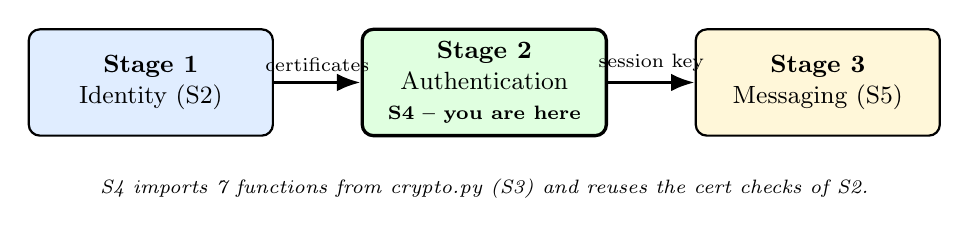
\begin{tikzpicture}[node distance=9mm and 11mm,every node/.style={font=\small},
    stage/.style={draw,rounded corners,minimum width=3.1cm,minimum height=1.35cm,
                  align=center,thick}]
  \node[stage,fill=boxblue]   (id)   {\textbf{Stage 1}\\Identity (S2)};
  \node[stage,fill=green!12,very thick,right=of id]   (auth)
       {\textbf{Stage 2}\\Authentication\\\scriptsize \textbf{S4 -- you are here}};
  \node[stage,fill=boxyellow,right=of auth] (msg) {\textbf{Stage 3}\\Messaging (S5)};
  \draw[-{Latex[length=3mm]},very thick] (id)   -- (auth)
       node[midway,above,font=\scriptsize]{certificates};
  \draw[-{Latex[length=3mm]},very thick] (auth) -- (msg)
       node[midway,above,font=\scriptsize]{session key};
  \node[below=4mm of auth,font=\scriptsize\itshape,align=center]
       {S4 imports 7 functions from crypto.py (S3) and reuses the cert checks of S2.};
\end{tikzpicture}
\end{center}

% =====================================================================
\section{The Theory You Must Study}
% =====================================================================

\subsection{Mutual Authentication}
\textbf{Plain definition.} \emph{Authentication} is proving who you are.
\emph{Mutual} authentication means \emph{both} parties prove their identity to
each other --- not just one side.

\textbf{Real-life analogy.} When you log in to a bank website, normally only
\emph{you} prove who you are (your password). Mutual authentication is stronger:
it is like meeting a courier where the courier shows you ID \emph{and} you show
the courier ID --- neither hands anything over until both are satisfied.

\textbf{Why it exists.} If only Vehicle~B checked Vehicle~A, an attacker could
impersonate B. If only A checked B, an attacker could impersonate A. A
man-in-the-middle relies on each side failing to check the other. Mutual
authentication closes both doors at once.

\textbf{How it works here.} In the handshake, B verifies A's certificate
\emph{and} A's signature, and A verifies B's certificate \emph{and} B's
signature. Both directions are checked before any safety message flows.

\textbf{Security property it provides.} \textbf{Authentication} (and, by
defeating MITM, it protects \textbf{confidentiality} and \textbf{integrity} too).

\subsection{Challenge--Response and the Handshake Nonce}
\textbf{Plain definition.} A \emph{challenge--response} is a test: one party
sends a fresh random value (the \emph{challenge}); the other must perform an
operation on it that only the genuine party could perform (the \emph{response}).
The fresh random value is a \textbf{nonce}.

\textbf{Real-life analogy.} A bouncer says ``say today's password backwards''.
Only someone who truly knows the password can do it, and because the request is
new each time, an eavesdropper who recorded yesterday's answer cannot reuse it.

\textbf{Why it exists.} Showing a certificate only proves the certificate is
real --- it does \emph{not} prove the sender \emph{owns} the matching private
key. A certificate is public; an attacker could copy it. The challenge--response
forces the sender to \emph{use} its private key on a value it could not have
predicted, proving live possession of the key.

\textbf{How it works here.} Each vehicle generates a 32-byte random nonce
(\texttt{os.urandom(32).hex()}). Each then \emph{signs} the pair of nonces with
its certificate private key (\texttt{ecdsa\_sign}). The other side verifies that
signature with the public key from the certificate (\texttt{ecdsa\_verify}). A
valid signature over a \emph{freshly chosen} nonce proves: ``you are online now
and you hold the private key''.

\textbf{Note on two kinds of nonce.} This 32-byte handshake nonce is \emph{not}
the same as the 12-byte AES-GCM nonce of S3. The handshake nonce is a freshness
challenge; the AES-GCM nonce makes each encryption unique. Same word, two jobs.

\textbf{Security property it provides.} \textbf{Authentication} and
\textbf{replay prevention}.

\subsection{Replay Attacks and the Replay Cache}
\textbf{Plain definition.} A \emph{replay attack} re-sends a previously captured,
genuine message. The \texttt{ReplayCache} is an in-memory list of nonces already
seen; a repeat is rejected.

\textbf{Real-life analogy.} A nightclub that ink-stamps each ticket as it is
used. A photocopied ticket carries a stamp number the door already recorded ---
entry refused.

\textbf{Why it exists.} Even a perfectly genuine, correctly signed HELLO becomes
dangerous if an attacker can record it and replay it later to start a bogus
session. The cache guarantees each nonce is accepted \emph{at most once}.

\textbf{How it works here.} \texttt{ReplayCache.check\_and\_add(nonce)} raises
\texttt{ReplayError} if the nonce is already stored, otherwise stores it with an
expiry of \texttt{now + 300\,s}. Old entries are cleaned out automatically. 300
seconds (5 minutes) is the constant \texttt{REPLAY\_WINDOW\_SECONDS}.

\textbf{Security property it provides.} \textbf{Replay prevention}.

\subsection{Timestamp / Freshness Validation}
\textbf{Plain definition.} Every handshake message carries the time it was
created. The \texttt{TimestampValidator} rejects any message whose time is too
far from ``now''.

\textbf{Real-life analogy.} A concert ticket printed with a date. The usher
glances at it: yesterday's ticket is refused on sight, without even checking the
seat number.

\textbf{Why it exists.} The replay cache only remembers nonces for 5 minutes and
costs memory. The timestamp check is a cheap first filter: a message hours old is
thrown out instantly. The two together are belt-and-braces.

\textbf{How it works here.} \texttt{TimestampValidator.validate(timestamp)}
computes \texttt{age = abs(now - timestamp)} and raises \texttt{StaleMessageError}
if \texttt{age > 5.0} seconds. Note the \texttt{abs}: a timestamp from the
\emph{future} is rejected too, which guards against clock-skew tricks.

\textbf{Security property it provides.} \textbf{Replay prevention}.

\subsection{Certificate Verification (recap from S2)}
The handshake must check that the certificate a peer presents was really signed
by the trusted CA. S4 does this with the helper
\texttt{verify\_certificate\_against\_ca}, which (1) parses the peer and CA
certificates, (2) verifies the CA's ECDSA-SHA256 signature on the peer
certificate, (3) checks the validity dates, and (4) returns the peer's public
key. This is the same logic explained fully in Section~S2 ---
S4 simply \emph{calls} it at the right moment. \emph{Security property:}
\textbf{authentication}.

\subsection{ECDH Ephemeral Key Exchange (recap from S3)}
During the handshake each vehicle generates a \emph{fresh} ECDH key pair
(\texttt{generate\_ecdh\_keypair}), sends the public half inside RESPONSE or ACK,
and combines its private half with the peer's public half
(\texttt{ecdh\_shared\_secret}) to get a shared secret. Both sides then run
\texttt{derive\_session\_key} (HKDF) to turn that secret plus the two nonces into
the \emph{same} 32-byte AES key. Because the ECDH keys are ephemeral, the session
has \textbf{forward secrecy}. The maths is covered in Section~S3.

\subsection{Dataclasses and the JSON Wire Format}
\textbf{Plain definition.} A Python \texttt{@dataclass} is a small class that
just holds named fields. \emph{JSON} (JavaScript Object Notation) is a simple
text format for structured data --- the form the messages take while crossing
the network.

\textbf{Real-life analogy.} A dataclass is a labelled paper form with named
boxes; \texttt{to\_json} folds the form into an envelope of text; \texttt{from\_json}
opens the envelope and reads the boxes back.

\textbf{Why it exists.} A network carries bytes, not Python objects. Each message
class has \texttt{to\_json()} (object $\to$ text) and \texttt{from\_json()} (text
$\to$ object), so a message can be sent and faithfully rebuilt on the far side.

\textbf{How it works here.} \texttt{HelloMessage}, \texttt{ChallengeMessage},
\texttt{ResponseMessage} and \texttt{AckMessage} are dataclasses. Each carries a
\texttt{msg\_type} tag (\texttt{"HELLO"}, \texttt{"CHALLENGE"}, ...) so the
receiver knows which form it has been handed. Binary values (nonces, signatures)
are carried as \emph{hex strings} because raw bytes cannot live inside JSON text.

\textbf{Security property it provides.} None directly --- it is the
\emph{format}, not a defence.

\subsection{Why Exactly Four Steps?}
Each step has a job, and you cannot remove one:
\begin{enumerate}
  \item \textbf{HELLO} --- A introduces itself and sends its certificate + nonce.
        (B can now check A's identity.)
  \item \textbf{CHALLENGE} --- B sends its certificate + nonce \emph{and} a
        signature over both nonces. (A can now check B's identity \emph{and}
        that B holds its private key.)
  \item \textbf{RESPONSE} --- A signs both nonces too, and sends its ephemeral
        ECDH public key. (B can now check A holds its key, and start the key
        exchange.)
  \item \textbf{ACK} --- B sends its ephemeral ECDH public key. (A can now finish
        the key exchange.)
\end{enumerate}
Steps 1--2 exchange certificates; steps 2--3 are the two-way challenge--response;
steps 3--4 exchange the ECDH public keys. Four messages is the minimum for
\emph{mutual} authentication plus a key agreement.

% =====================================================================
\section{Code Walkthrough}
% =====================================================================

\texttt{auth\_protocol.py} has four parts: custom exceptions, four message
dataclasses, two small protection classes (\texttt{ReplayCache},
\texttt{TimestampValidator}), the certificate helper, and the main
\texttt{AuthProtocol} class.

\subsection{The custom exceptions}
\begin{lstlisting}[style=py,caption={auth\_protocol.py --- the exception hierarchy.}]
class AuthError(Exception):
    """Base exception for authentication errors."""

class ReplayError(AuthError):
    """Raised when a replayed nonce is detected."""

class StaleMessageError(AuthError):
    """Raised when a message timestamp is too old."""

class CertificateError(AuthError):
    """Raised when certificate verification fails."""
\end{lstlisting}
\textbf{Explanation:} \texttt{AuthError} is the parent; the three children name
the three specific ways a handshake can be rejected --- a replayed nonce, a stale
message, a bad certificate. Naming each one separately makes the failure reason
obvious in logs and in the attack demos.

\subsection{The four message dataclasses}
\begin{lstlisting}[style=py,caption={auth\_protocol.py --- the HELLO message (the
other three messages follow the same pattern).}]
@dataclass
class HelloMessage:
    vehicle_id: str
    certificate_pem: str
    nonce: str
    timestamp: float
    msg_type: str = "HELLO"

    def to_json(self) -> str:
        return json.dumps(asdict(self))

    @classmethod
    def from_json(cls, data: str) -> HelloMessage:
        return cls(**json.loads(data))
\end{lstlisting}
\textbf{Step by step:}
\begin{enumerate}
  \item The \texttt{@dataclass} decorator auto-generates the boring boilerplate
        (constructor, etc.) so the class is just a list of named fields.
  \item \texttt{HelloMessage} fields: the sender's \texttt{vehicle\_id}, its
        \texttt{certificate\_pem} (its passport as text), its \texttt{nonce}
        (32 random bytes as a 64-character hex string), the \texttt{timestamp},
        and a fixed \texttt{msg\_type} tag.
  \item \texttt{to\_json} turns the object into a JSON text string ready to send.
  \item \texttt{from\_json} is a \emph{classmethod} that rebuilds the object from
        a received JSON string.
\end{enumerate}
The other three dataclasses differ only in their fields:
\begin{itemize}
  \item \texttt{ChallengeMessage} adds \texttt{signed\_nonces} (an ECDSA
        signature over both nonces, as hex).
  \item \texttt{ResponseMessage} carries \texttt{signed\_nonces} and
        \texttt{ecdh\_public\_key\_pem} (the ephemeral ECDH public key) ---
        note it has \emph{no} certificate field, because A already sent its
        certificate in HELLO.
  \item \texttt{AckMessage} carries only \texttt{ecdh\_public\_key\_pem} and a
        \texttt{session\_established} flag --- and, unlike the others, it has
        \emph{no timestamp field}.
\end{itemize}

\subsection{ReplayCache --- catching repeated nonces}
\begin{lstlisting}[style=py,caption={auth\_protocol.py --- the replay cache.}]
class ReplayCache:
    def __init__(self, window_seconds: int = 300) -> None:
        self._window = window_seconds
        self._seen: dict[str, float] = {}   # {nonce_hex: expiry_timestamp}

    def check_and_add(self, nonce: str) -> None:
        self._cleanup()
        if nonce in self._seen:
            raise ReplayError(f"Nonce already seen: {nonce[:16]}...")
        self._seen[nonce] = time.time() + self._window

    def _cleanup(self) -> None:
        now = time.time()
        expired = [n for n, exp in self._seen.items() if exp < now]
        for n in expired:
            del self._seen[n]
\end{lstlisting}
\textbf{Step by step:}
\begin{enumerate}
  \item \texttt{\_\_init\_\_} sets the remembering window (default 300\,s) and an
        empty dictionary \texttt{\_seen} mapping each nonce to the time it should
        be forgotten.
  \item \texttt{check\_and\_add} first calls \texttt{\_cleanup}.
  \item If the nonce is already in \texttt{\_seen}, it raises \texttt{ReplayError}
        --- this is a replay attack being caught.
  \item Otherwise it records the nonce with expiry \texttt{now + 300\,s}.
  \item \texttt{\_cleanup} deletes nonces whose expiry has passed, so the cache
        does not grow forever.
\end{enumerate}
\textbf{Arguments:} \texttt{nonce} (hex string). \textbf{Returns:} nothing.
\textbf{Exceptions:} \texttt{ReplayError}. \emph{Analogy:} the ink-stamp register
at the nightclub door.

\subsection{TimestampValidator --- catching stale messages}
\begin{lstlisting}[style=py,caption={auth\_protocol.py --- the timestamp validator.}]
class TimestampValidator:
    def __init__(self, max_age_seconds: float = 5.0) -> None:
        self._max_age = max_age_seconds

    def validate(self, timestamp: float) -> None:
        age = abs(time.time() - timestamp)
        if age > self._max_age:
            raise StaleMessageError(
                f"Message is {age:.1f}s old (max {self._max_age}s)"
            )
\end{lstlisting}
\textbf{Step by step:}
\begin{enumerate}
  \item \texttt{\_\_init\_\_} stores the maximum allowed age (default 5.0\,s).
  \item \texttt{validate} computes the \emph{absolute} difference between now and
        the message's timestamp.
  \item If that age exceeds 5 seconds, it raises \texttt{StaleMessageError}.
\end{enumerate}
\textbf{Why \texttt{abs}?} It rejects both \emph{too-old} messages (a real replay)
and \emph{too-future} messages (a forged or clock-skewed timestamp).
\emph{Analogy:} the usher refusing a ticket whose date is not today.

\subsection{verify\_certificate\_against\_ca --- the certificate gate}
\begin{lstlisting}[style=py,caption={auth\_protocol.py --- verify a peer certificate against the trusted CA.}]
def verify_certificate_against_ca(cert_pem, ca_cert_pem):
    try:
        cert_bytes = cert_pem.encode("utf-8") if isinstance(cert_pem, str) else cert_pem
        cert = x509.load_pem_x509_certificate(cert_bytes)
        ca_cert = x509.load_pem_x509_certificate(ca_cert_pem)

        # Verify the CA's signature on the vehicle certificate.
        ca_public_key = ca_cert.public_key()
        ca_public_key.verify(
            cert.signature,
            cert.tbs_certificate_bytes,
            ec.ECDSA(hashes.SHA256()),
        )

        # Check validity dates (now must be inside the window).
        now = datetime.now(timezone.utc)
        nb = getattr(cert, "not_valid_before_utc", None) or \
             cert.not_valid_before.replace(tzinfo=timezone.utc)
        na = getattr(cert, "not_valid_after_utc", None) or \
             cert.not_valid_after.replace(tzinfo=timezone.utc)
        if now < nb: raise CertificateError("Certificate is not yet valid")
        if now > na: raise CertificateError("Certificate has expired")

        pub_key = cert.public_key()
        if not isinstance(pub_key, ec.EllipticCurvePublicKey):
            raise CertificateError("Certificate does not contain an EC public key")
        return pub_key
    except CertificateError:
        raise
    except Exception as exc:
        raise CertificateError(f"Certificate verification failed: {exc}") from exc
\end{lstlisting}
\textbf{Step by step:}
\begin{enumerate}
  \item Parse the peer's certificate and the CA's certificate from PEM text.
  \item \texttt{ca\_public\_key.verify(...)} checks the CA's ECDSA-SHA256
        signature on the peer certificate's \texttt{tbs\_certificate\_bytes}
        (the ``to-be-signed'' body). A forged certificate fails here.
  \item Check that ``now'' is inside the certificate's validity window;
        otherwise raise \texttt{CertificateError}.
  \item Confirm the embedded public key is an elliptic-curve key, then
        \textbf{return} it --- the caller needs it to verify signatures.
  \item Any failure becomes a \texttt{CertificateError}.
\end{enumerate}
\textbf{Theory link:} certificate verification / chain of trust (S2). This is the
first of the two identity checks; the second is the signature challenge.

\subsection{The AuthProtocol class}

\subsubsection*{\_\_init\_\_ --- set up one vehicle's handshake state}
The constructor stores the vehicle's id, its private key, its certificate (PEM
bytes), and the CA certificate. It creates one \texttt{ReplayCache} and one
\texttt{TimestampValidator}, and prepares empty ``slots'' for the handshake
state: \texttt{my\_nonce}, \texttt{peer\_nonce}, \texttt{peer\_public\_key},
\texttt{session\_key}, and the ephemeral ECDH key pair. Both vehicles create one
\texttt{AuthProtocol} object each.

\subsubsection*{Step 1 --- build\_hello() (initiator)}
\begin{lstlisting}[style=py,caption={auth\_protocol.py --- Step 1: build the HELLO.}]
def build_hello(self) -> HelloMessage:
    self.my_nonce = os.urandom(32).hex()
    hello = HelloMessage(
        vehicle_id=self.vehicle_id,
        certificate_pem=self.certificate_pem.decode("utf-8"),
        nonce=self.my_nonce,
        timestamp=time.time(),
    )
    return hello
\end{lstlisting}
\textbf{Steps:} (1) generate a fresh 32-byte random nonce, stored as hex in
\texttt{my\_nonce}; (2) build a \texttt{HelloMessage} carrying the vehicle id,
the certificate, the nonce and the current time; (3) return it to be sent.
\textbf{Theory link:} starts the challenge--response by issuing this vehicle's
challenge nonce.

\subsubsection*{Step 2 --- process\_hello() (responder)}
\begin{lstlisting}[style=py,caption={auth\_protocol.py --- Step 2: verify HELLO, build CHALLENGE.}]
def process_hello(self, msg: HelloMessage) -> ChallengeMessage:
    # 1. Reject stale messages
    self.timestamp_validator.validate(msg.timestamp)
    # 2. Reject replayed nonces
    self.replay_cache.check_and_add(msg.nonce)
    # 3. Verify peer certificate was signed by our trusted CA
    self.peer_public_key = verify_certificate_against_ca(
        msg.certificate_pem, self.ca_cert_pem)
    # 4. Store peer nonce; generate our own
    self.peer_nonce = msg.nonce
    self.my_nonce = os.urandom(32).hex()
    # 5. Sign (peer_nonce + our_nonce) -- proves private key possession
    nonce_data = bytes.fromhex(self.peer_nonce) + bytes.fromhex(self.my_nonce)
    signature = ecdsa_sign(self.private_key, nonce_data)
    challenge = ChallengeMessage(
        vehicle_id=self.vehicle_id,
        certificate_pem=self.certificate_pem.decode("utf-8"),
        nonce=self.my_nonce,
        signed_nonces=signature.hex(),
        timestamp=time.time(),
    )
    return challenge
\end{lstlisting}
\textbf{Step by step:}
\begin{enumerate}
  \item Validate the HELLO's timestamp --- reject if older than 5 seconds.
  \item Replay-check the HELLO's nonce --- reject if seen before.
  \item Verify A's certificate against the CA; on success, store A's public key.
  \item Save A's nonce as \texttt{peer\_nonce}; generate this vehicle's own fresh
        nonce.
  \item Join the two nonces into bytes and \emph{sign} them with this vehicle's
        private key. This signature is the response to A's challenge \emph{and}
        a new challenge to A.
  \item Build and return the CHALLENGE carrying B's certificate, B's nonce, the
        signature, and a timestamp.
\end{enumerate}
\textbf{Theory link:} certificate verification + the responding half of
challenge--response. \emph{Analogy:} the bouncer checks A's ID, then says ``now
\emph{you} repeat \emph{my} password too.''

\subsubsection*{Step 3 --- process\_challenge() (initiator)}
\begin{lstlisting}[style=py,caption={auth\_protocol.py --- Step 3: verify CHALLENGE, build RESPONSE.}]
def process_challenge(self, msg: ChallengeMessage) -> ResponseMessage:
    self.timestamp_validator.validate(msg.timestamp)
    self.replay_cache.check_and_add(msg.nonce)
    # Verify peer certificate
    self.peer_public_key = verify_certificate_against_ca(
        msg.certificate_pem, self.ca_cert_pem)
    # Verify peer's signature on (our_nonce + their_nonce)
    self.peer_nonce = msg.nonce
    expected_data = bytes.fromhex(self.my_nonce) + bytes.fromhex(self.peer_nonce)
    if not ecdsa_verify(self.peer_public_key, expected_data,
                        bytes.fromhex(msg.signed_nonces)):
        raise AuthError("Challenge signature invalid -- possible impersonation")
    # Generate ephemeral ECDH key pair (forward secrecy)
    self._ecdh_private, self._ecdh_public = generate_ecdh_keypair()
    # Sign nonces with OUR private key
    our_sig = ecdsa_sign(self.private_key, expected_data)
    response = ResponseMessage(
        signed_nonces=our_sig.hex(),
        ecdh_public_key_pem=serialize_public_key(self._ecdh_public).decode("utf-8"),
        timestamp=time.time(),
    )
    return response
\end{lstlisting}
\textbf{Step by step:}
\begin{enumerate}
  \item Validate the CHALLENGE timestamp and replay-check B's nonce.
  \item Verify B's certificate against the CA; store B's public key.
  \item Re-build the exact nonce pair B claims to have signed
        (\texttt{my\_nonce + peer\_nonce}) and check B's signature with
        \texttt{ecdsa\_verify}. If it fails, raise \texttt{AuthError} ---
        ``possible impersonation''. \emph{This is where a fake B is caught.}
  \item Generate this vehicle's \emph{ephemeral} ECDH key pair (forward secrecy).
  \item Sign the same nonce pair with this vehicle's certificate private key ---
        the response to B's challenge.
  \item Build and return the RESPONSE carrying the signature and the ECDH public
        key (as PEM text).
\end{enumerate}
\textbf{Theory link:} verifying the challenge response = the second identity
check; \texttt{generate\_ecdh\_keypair} starts the key agreement.

\subsubsection*{Step 4a --- process\_response() (responder)}
\begin{lstlisting}[style=py,caption={auth\_protocol.py --- Step 4a: verify RESPONSE, derive key, build ACK.}]
def process_response(self, msg: ResponseMessage, original_hello: HelloMessage) -> AckMessage:
    self.timestamp_validator.validate(msg.timestamp)
    # Verify initiator's signature on (their_nonce + our_nonce)
    nonce_data = bytes.fromhex(self.peer_nonce) + bytes.fromhex(self.my_nonce)
    if not ecdsa_verify(self.peer_public_key, nonce_data,
                        bytes.fromhex(msg.signed_nonces)):
        raise AuthError("Response signature invalid")
    # Generate our ECDH key pair and compute shared secret
    self._ecdh_private, self._ecdh_public = generate_ecdh_keypair()
    peer_ecdh_pub = load_public_key(msg.ecdh_public_key_pem.encode("utf-8"))
    shared_secret = ecdh_shared_secret(self._ecdh_private, peer_ecdh_pub)
    # Derive session key -- initiator nonce first for consistency
    nonce_a = bytes.fromhex(self.peer_nonce)   # initiator's nonce
    nonce_b = bytes.fromhex(self.my_nonce)     # our nonce (responder)
    self.session_key = derive_session_key(shared_secret, nonce_a, nonce_b)
    ack = AckMessage(
        ecdh_public_key_pem=serialize_public_key(self._ecdh_public).decode("utf-8"),
    )
    return ack
\end{lstlisting}
\textbf{Step by step:}
\begin{enumerate}
  \item Validate the RESPONSE timestamp.
  \item Verify A's signature over the nonce pair (\texttt{peer\_nonce +
        my\_nonce}). Fail $\to$ \texttt{AuthError}. Now B is sure A holds A's
        private key.
  \item Generate B's ephemeral ECDH key pair; load A's ECDH public key from the
        RESPONSE; compute the ECDH shared secret.
  \item Derive the session key with HKDF, putting the \emph{initiator's} nonce
        first (\texttt{nonce\_a}) and the \emph{responder's} second
        (\texttt{nonce\_b}) --- a fixed order so both sides agree.
  \item Build and return the ACK carrying B's ECDH public key.
\end{enumerate}
\textbf{Honest note:} the parameter \texttt{original\_hello} is part of the
signature but is not actually used inside the method body --- the demo passes the
HELLO object anyway. Worth mentioning if an examiner asks.

\subsubsection*{Step 4b --- process\_ack() (initiator)}
\begin{lstlisting}[style=py,caption={auth\_protocol.py --- Step 4b: process ACK, derive the matching key.}]
def process_ack(self, msg: AckMessage) -> bytes:
    peer_ecdh_pub = load_public_key(msg.ecdh_public_key_pem.encode("utf-8"))
    shared_secret = ecdh_shared_secret(self._ecdh_private, peer_ecdh_pub)
    # Same nonce order as the responder used
    nonce_a = bytes.fromhex(self.my_nonce)     # initiator's nonce (us)
    nonce_b = bytes.fromhex(self.peer_nonce)   # responder's nonce
    self.session_key = derive_session_key(shared_secret, nonce_a, nonce_b)
    return self.session_key
\end{lstlisting}
\textbf{Step by step:}
\begin{enumerate}
  \item Load B's ECDH public key from the ACK.
  \item Compute the ECDH shared secret from A's ephemeral private key and B's
        ephemeral public key. By ECDH maths this equals the secret B computed.
  \item Derive the session key with HKDF --- and crucially with the \emph{same
        nonce order} B used (initiator's nonce first). Same secret + same nonces
        + same HKDF $\Rightarrow$ \emph{identical 32-byte key}.
  \item Return the session key. The handshake is complete.
\end{enumerate}
\textbf{Theory link:} ECDH + HKDF (S3). \emph{Analogy:} both painters reach the
same final colour --- and both label the tin the same way, so they truly match.

\subsubsection*{The demo block}
The \texttt{if \_\_name\_\_ == "\_\_main\_\_"} block at the bottom loads the CA
and both vehicle certificates, creates two \texttt{AuthProtocol} objects, and
runs the five calls in order: \texttt{build\_hello} $\to$ \texttt{process\_hello}
$\to$ \texttt{process\_challenge} $\to$ \texttt{process\_response} $\to$
\texttt{process\_ack}. It then prints both session keys and confirms they match.
\emph{In this demo the two objects call each other's methods directly in one
process; in the real system (S6) the messages travel over TCP between two
programs.}

% =====================================================================
\section{Hands-On / Practical}
% =====================================================================

\subsection{Run the handshake by itself}
The handshake demo needs the certificates first (Section~S2). Run, in order:
\begin{lstlisting}[style=term]
python ca\ca.py
python ca\issue_cert.py --vehicle-id vehicle-a --output-dir ca\certs
python ca\issue_cert.py --vehicle-id vehicle-b --output-dir ca\certs
python protocol\auth_protocol.py
\end{lstlisting}

\noindent\textbf{Expected output (sample). Where this guide shows \texttt{[OK]}
the real terminal prints a small check-mark character.}
\begin{lstlisting}[style=term]
=== V2V AUTHENTICATION HANDSHAKE DEMO ===

[10:00:00] INFO: [vehicle-a] Sent HELLO (nonce=3f1a9c2e...)
[10:00:00] INFO: [vehicle-b] Received HELLO from vehicle-a
[10:00:00] INFO: [vehicle-b] Certificate VALID for vehicle-a
[10:00:00] INFO: [vehicle-b] Sent CHALLENGE (nonce=8b4d77e1...)
[10:00:00] INFO: [vehicle-a] Received CHALLENGE from vehicle-b
[10:00:00] INFO: [vehicle-a] Certificate VALID for vehicle-b
[10:00:00] INFO: [vehicle-a] Challenge signature verified [OK]
[10:00:00] INFO: [vehicle-a] Sent RESPONSE with ECDH public key
[10:00:00] INFO: [vehicle-b] Received RESPONSE
[10:00:00] INFO: [vehicle-b] Response signature verified [OK]
[10:00:00] INFO: [vehicle-b] Session key derived (forward secrecy: ENABLED)
[10:00:00] INFO: [vehicle-b] Sent ACK -- handshake complete (responder)
[10:00:00] INFO: [vehicle-a] Received ACK -- session established
[10:00:00] INFO: [vehicle-a] MUTUAL AUTHENTICATION COMPLETE -- session key derived

Vehicle A session key: 1c9e7a4f0b2d6688...
Vehicle B session key: 1c9e7a4f0b2d6688...
Keys match: True
Handshake time: 7.3 ms
[OK] Mutual authentication successful - both vehicles share the same key!
\end{lstlisting}

\subsection{What the output lines mean}
\begin{itemize}
  \item \texttt{Sent HELLO} --- Step 1: A issued its nonce.
  \item \texttt{Certificate VALID} (twice) --- each side confirmed the other's
        passport was signed by the CA.
  \item \texttt{Challenge/Response signature verified} --- each side proved it
        \emph{owns} its private key (the challenge--response succeeded).
  \item \texttt{Session key derived (forward secrecy: ENABLED)} --- the ephemeral
        ECDH exchange produced the key.
  \item \texttt{Keys match: True} --- the whole point: both sides hold the
        \emph{identical} key, though it was never transmitted.
\end{itemize}

\subsection{Try This Yourself (three ways to break the handshake)}
Open \texttt{auth\_protocol.py} and edit the demo block at the bottom.

\textbf{Experiment 1 --- replayed nonce.} After the line
\texttt{challenge = auth\_b.process\_hello(hello)} add a second identical call:
\begin{lstlisting}[style=term]
challenge = auth_b.process_hello(hello)
auth_b.process_hello(hello)         # <-- feed the SAME hello again
\end{lstlisting}
\textbf{Predict:} the first call stored the HELLO's nonce; the second call finds
it already in the \texttt{ReplayCache} and raises \texttt{ReplayError: Nonce
already seen}. This is exactly the replay defence.

\textbf{Experiment 2 --- stale message.} Before \texttt{process\_hello}, age the
HELLO by editing its timestamp:
\begin{lstlisting}[style=term]
hello = auth_a.build_hello()
hello.timestamp = hello.timestamp - 100   # pretend it is 100 s old
challenge = auth_b.process_hello(hello)
\end{lstlisting}
\textbf{Predict:} \texttt{TimestampValidator} sees an age of about 100 seconds
($> 5$) and raises \texttt{StaleMessageError}.

\textbf{Experiment 3 --- bad signature (impersonation).} Corrupt the challenge
signature before A processes it:
\begin{lstlisting}[style=term]
challenge.signed_nonces = "00" + challenge.signed_nonces[2:]
response = auth_a.process_challenge(challenge)
\end{lstlisting}
\textbf{Predict:} \texttt{ecdsa\_verify} returns \texttt{False}, so
\texttt{process\_challenge} raises \texttt{AuthError: Challenge signature invalid
-- possible impersonation}. \textbf{Undo all edits afterwards.}

% =====================================================================
\section{Attack Relevance}
% =====================================================================

S4 is the busiest defensive section: it stops \emph{three} of the four attacks
and is exercised by both \texttt{attacks/replay\_attack.py} and
\texttt{attacks/mitm\_attack.py}.

\begin{table}[h]
\centering
\small
\begin{tabular}{@{}p{2.5cm} p{6.0cm} p{5.0cm}@{}}
\toprule
\textbf{Attack} & \textbf{How S4 stops it} & \textbf{The mechanism}\\
\midrule
Replay & A captured HELLO/CHALLENGE is re-sent; its nonce is already in the
cache, or its timestamp is too old. & \texttt{ReplayCache.check\_and\_add},
\texttt{TimestampValidator.validate}.\\
MITM (fake cert) & The attacker's certificate is not signed by the CA. &
\texttt{verify\_certificate\_against\_ca} raises \texttt{CertificateError}.\\
MITM / Impersonation (forged signature) & The attacker cannot sign the fresh
nonce pair without the real private key. & \texttt{ecdsa\_verify} returns
\texttt{False} $\to$ \texttt{AuthError}.\\
\bottomrule
\end{tabular}
\caption{S4 defeats replay, fake-certificate MITM, and impersonation.}
\end{table}

\noindent\textbf{Why the handshake defeats a man-in-the-middle.} An MITM attacker
sits between A and B. To impersonate A to B, the attacker must send a CHALLENGE
or RESPONSE that B accepts. Two walls block this:
\begin{enumerate}
  \item \textbf{The certificate wall.} The attacker's certificate must be
        CA-signed. A self-signed forgery fails
        \texttt{verify\_certificate\_against\_ca}.
  \item \textbf{The signature wall.} Even if the attacker \emph{replays} A's real
        certificate, it must then sign the \emph{fresh} nonce pair B just chose.
        Signing needs A's private key, which the attacker does not have. So
        \texttt{ecdsa\_verify} fails and the handshake aborts.
\end{enumerate}
This is why S2 (identity) alone is not enough and S4 is needed: S2 proves a
certificate is genuine; S4's challenge--response proves the sender \emph{owns}
the matching private key \emph{right now}.

\textbf{Forward secrecy contribution.} Because the ECDH keys are ephemeral
(\texttt{generate\_ecdh\_keypair} per session), even an attacker who later steals
a vehicle's \emph{certificate} private key cannot reconstruct a past session key
--- the ephemeral keys that built it no longer exist.

\textbf{Honest scope note.} The handshake assumes clocks are roughly
synchronised (within 5\,s) for the timestamp check; on badly skewed clocks an
honest handshake could be wrongly rejected. Also, the demo wires the two objects
together in one process --- real networking, framing and threading are added in
Section~S6.

% =====================================================================
\section{Illustrations}
% =====================================================================

\subsection{Diagram 1 --- The 4-Step Handshake (message flow)}
\begin{center}
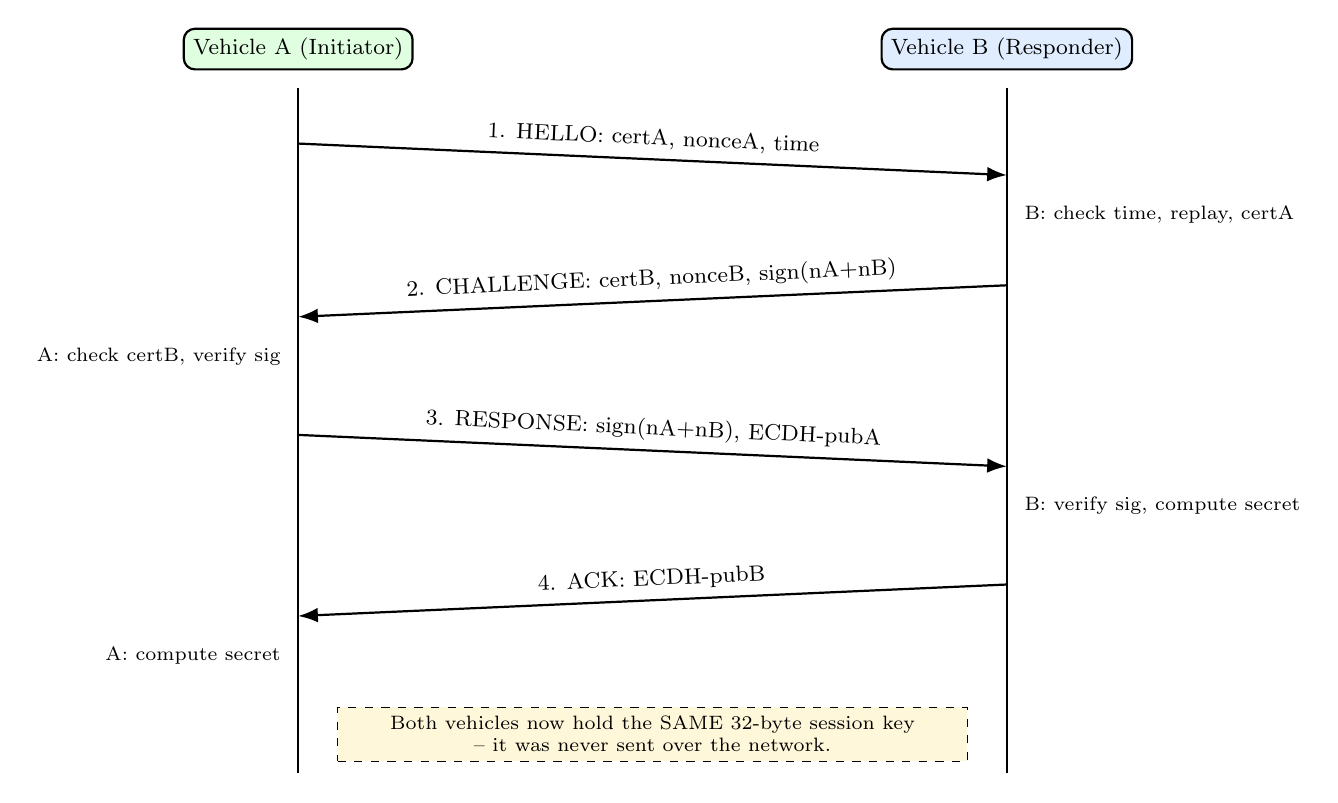
\begin{tikzpicture}[font=\footnotesize]
  % lifelines
  \node[draw,thick,rounded corners,fill=green!12] (A) at (0,0)
       {Vehicle A (Initiator)};
  \node[draw,thick,rounded corners,fill=boxblue] (B) at (9,0)
       {Vehicle B (Responder)};
  \draw[thick] (0,-0.5) -- (0,-9.2);
  \draw[thick] (9,-0.5) -- (9,-9.2);
  % step 1
  \draw[-{Latex[length=2.5mm]},thick] (0,-1.2) -- (9,-1.6)
       node[midway,above,sloped]{1. HELLO: certA, nonceA, time};
  \node[right=1mm,align=left,font=\scriptsize] at (9,-2.1)
       {B: check time, replay, certA};
  % step 2
  \draw[-{Latex[length=2.5mm]},thick] (9,-3.0) -- (0,-3.4)
       node[midway,above,sloped]{2. CHALLENGE: certB, nonceB, sign(nA+nB)};
  \node[left=1mm,align=right,font=\scriptsize] at (0,-3.9)
       {A: check certB, verify sig};
  % step 3
  \draw[-{Latex[length=2.5mm]},thick] (0,-4.9) -- (9,-5.3)
       node[midway,above,sloped]{3. RESPONSE: sign(nA+nB), ECDH-pubA};
  \node[right=1mm,align=left,font=\scriptsize] at (9,-5.8)
       {B: verify sig, compute secret};
  % step 4
  \draw[-{Latex[length=2.5mm]},thick] (9,-6.8) -- (0,-7.2)
       node[midway,above,sloped]{4. ACK: ECDH-pubB};
  \node[left=1mm,align=right,font=\scriptsize] at (0,-7.7)
       {A: compute secret};
  % result
  \node[draw,dashed,fill=boxyellow,minimum width=8cm,align=center,font=\scriptsize]
       at (4.5,-8.7)
       {Both vehicles now hold the SAME 32-byte session key\\
        -- it was never sent over the network.};
\end{tikzpicture}
\end{center}

\subsection{Diagram 2 --- The three gates every handshake message passes}
\begin{center}
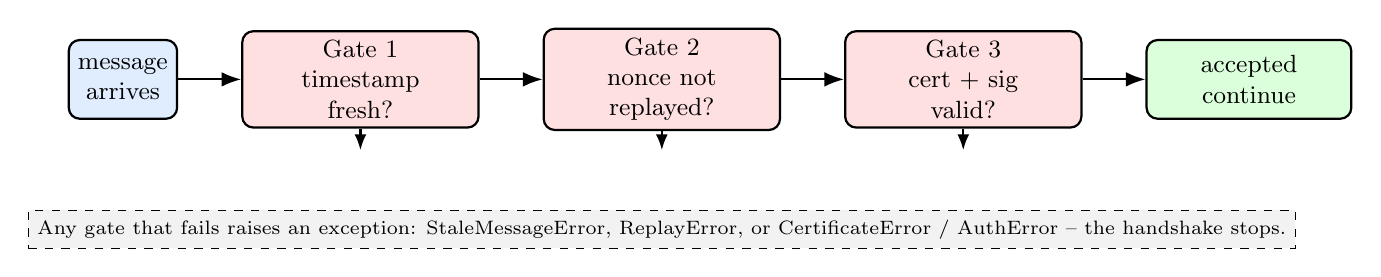
\begin{tikzpicture}[font=\small,node distance=7mm,
   gate/.style={draw,thick,rounded corners,minimum width=3.0cm,minimum height=1.0cm,
                align=center,fill=red!12},
   ok/.style={draw,thick,rounded corners,minimum width=2.6cm,minimum height=1.0cm,
              align=center,fill=green!14}]
  \node[draw,thick,rounded corners,fill=boxblue,minimum height=1cm,align=center] (in) {message\\arrives};
  \node[gate,right=8mm of in] (g1) {Gate 1\\timestamp\\fresh?};
  \node[gate,right=8mm of g1] (g2) {Gate 2\\nonce not\\replayed?};
  \node[gate,right=8mm of g2] (g3) {Gate 3\\cert + sig\\valid?};
  \node[ok,right=8mm of g3] (acc) {accepted\\continue};
  \draw[-{Latex[length=2.5mm]},thick] (in) -- (g1);
  \draw[-{Latex[length=2.5mm]},thick] (g1) -- (g2);
  \draw[-{Latex[length=2.5mm]},thick] (g2) -- (g3);
  \draw[-{Latex[length=2.5mm]},thick] (g3) -- (acc);
  \node[below=10mm of g2,draw,dashed,fill=gray!10,minimum width=9cm,
        align=center,font=\scriptsize]
       {Any gate that fails raises an exception: StaleMessageError,
        ReplayError, or CertificateError / AuthError -- the handshake stops.};
  \draw[-{Latex[length=2mm]},thick] (g1) -- ++(0,-0.9);
  \draw[-{Latex[length=2mm]},thick] (g2) -- ++(0,-0.9);
  \draw[-{Latex[length=2mm]},thick] (g3) -- ++(0,-0.9);
\end{tikzpicture}
\end{center}

% =====================================================================
\section{Presentation Pack}
% =====================================================================

\subsection{Slide Outline}

\textbf{Slide 1 --- Why a Handshake?}
\begin{itemize}
  \item Before any safety message, the cars must trust each other.
  \item Showing a certificate is not enough --- certificates are public.
  \item The handshake adds a live ``prove you own the key'' test.
  \item It also secretly agrees on a shared encryption key.
\end{itemize}

\textbf{Slide 2 --- The Four Steps.}
\begin{itemize}
  \item HELLO: A sends its certificate + a random nonce.
  \item CHALLENGE: B sends its certificate + nonce + a signature.
  \item RESPONSE: A sends its signature + an ECDH public key.
  \item ACK: B sends its ECDH public key --- done.
\end{itemize}

\textbf{Slide 3 --- Challenge--Response: Proving Key Ownership.}
\begin{itemize}
  \item Each side signs the pair of fresh nonces with its private key.
  \item The other side verifies with the certificate's public key.
  \item A valid signature over a brand-new nonce = ``you own the key, now''.
  \item Wrong/missing key $\to$ \texttt{AuthError} --- impersonation caught.
\end{itemize}

\textbf{Slide 4 --- Three Gates Stop Replay.}
\begin{itemize}
  \item Timestamp gate: message older than 5\,s $\to$ \texttt{StaleMessageError}.
  \item Nonce gate: nonce seen before $\to$ \texttt{ReplayError}.
  \item Certificate gate: not CA-signed $\to$ \texttt{CertificateError}.
  \item Belt-and-braces: cheap time check plus exact-duplicate check.
\end{itemize}

\textbf{Slide 5 --- A Shared Key, Never Sent.}
\begin{itemize}
  \item Each side makes an ephemeral ECDH key pair.
  \item Public halves are swapped in RESPONSE and ACK.
  \item Both compute the same secret; HKDF turns it into a 32-byte key.
  \item Ephemeral keys $\to$ forward secrecy. ``Keys match: True''.
\end{itemize}

\subsection{Speaker Talking Points (about 30--60 seconds each)}

\textbf{Slide 1.} ``Before our two cars send a single safety message, they run a
handshake --- a short, fixed four-step conversation. Why bother? Because simply
showing a certificate is not enough. A certificate is public; anyone can copy it.
So the handshake does two extra jobs. First, it makes each car prove, live, that
it actually \emph{owns} the private key behind its certificate --- not just that
it has a copy of the certificate. Second, while doing that, the two cars secretly
agree on a shared encryption key. By the end, each car is certain who it is
talking to and they share a secret nobody else knows.''

\textbf{Slide 2.} ``The handshake has four messages. In HELLO, car A introduces
itself, sending its certificate and a fresh random number called a nonce. In
CHALLENGE, car B replies with its own certificate, its own nonce, and --
importantly -- a digital signature over both nonces. In RESPONSE, car A signs
both nonces too and includes a special temporary key for the key exchange.
Finally in ACK, car B sends its matching temporary key. Four messages: two to
swap certificates, and the signatures going both ways for the proof.''

\textbf{Slide 3.} ``The heart of the handshake is challenge--response. Each car
picks a brand-new random nonce that the other side could not have predicted. Each
car then signs the pair of nonces with its private key. The other side verifies
that signature using the public key inside the certificate. Here is the clever
part: because the nonce is fresh, a recorded old signature is useless, and
because signing needs the private key, only the genuine car can produce a
signature that verifies. If the signature is wrong, our code raises an AuthError
and says `possible impersonation'. That single check is what stops a fake car.''

\textbf{Slide 4.} ``Every handshake message passes three gates. The first gate
checks the timestamp --- if the message is more than five seconds old, it is
stale and rejected immediately; that is cheap and fast. The second gate checks
the nonce against a replay cache --- if we have seen that exact nonce before, it
is a replay and we reject it. The third gate checks the certificate is signed by
our trusted CA. Any gate failing throws a specific exception and the handshake
stops. Two of those gates --- timestamp and nonce --- together make replaying an
old handshake impossible.''

\textbf{Slide 5.} ``Finally, the key. During the handshake each car generates a
temporary, throw-away key pair for something called ECDH. They swap only the
\emph{public} halves, inside the RESPONSE and ACK messages. Then each car
combines its own private half with the other's public half, and thanks to the
maths both end up with the \emph{same} secret --- even though that secret was
never sent. HKDF turns it into a clean 32-byte key. And because those ECDH keys
are thrown away after the session, even a key stolen later cannot unlock this
conversation --- that is forward secrecy. The demo ends by printing `Keys match:
True'.''

\subsection{Live-Demo Script}
\begin{enumerate}
  \item \textbf{Set up.} Run \texttt{ca.py} and the two \texttt{issue\_cert.py}
        commands so the certificates exist.
  \item \textbf{Run the handshake.} Execute \texttt{python
        protocol\textbackslash auth\_protocol.py}. Read the log aloud, pointing
        at each of the four steps in turn.
  \item \textbf{Point at the proof lines.} ``Certificate VALID'' (the cert gate)
        and ``signature verified'' (the challenge--response).
  \item \textbf{Point at the result.} ``Keys match: True'' --- ``the same key on
        both sides, never sent over the wire.''
  \item \textbf{Break it live.} Apply Experiment~1 (replay) or Experiment~3 (bad
        signature) from the Hands-On section and show the \texttt{ReplayError} or
        \texttt{AuthError}. Restore the file afterwards.
\end{enumerate}

\subsection{Examiner Q\&A}
\begin{enumerate}
  \item \textbf{Q: What is mutual authentication and why not just one-sided?}\\
        A: Both parties prove identity to each other. One-sided authentication
        leaves the unchecked side open to impersonation and enables a
        man-in-the-middle; mutual authentication checks both directions.
  \item \textbf{Q: A certificate is already trusted --- why also do
        challenge--response?}\\
        A: A certificate is public and can be copied. The challenge--response
        forces the sender to sign a \emph{fresh, unpredictable} nonce with the
        private key, proving it \emph{owns} the key right now, not just holds a
        copy of the certificate.
  \item \textbf{Q: Why are there two nonces, one from each side?}\\
        A: So that \emph{each} side issues a challenge the \emph{other} must
        answer. Both nonces are signed, giving a two-way proof, and both feed
        HKDF so the session key is bound to this exact exchange.
  \item \textbf{Q: How does the handshake stop a replayed HELLO?}\\
        A: Two ways: \texttt{TimestampValidator} rejects it if older than 5\,s,
        and \texttt{ReplayCache} rejects it if its nonce was already seen
        (remembered for 300\,s).
  \item \textbf{Q: How is the session key the same on both sides if it is never
        sent?}\\
        A: ECDH: each side combines its ephemeral private key with the peer's
        ephemeral public key to get the identical shared secret; both then run
        HKDF with the same nonce order, producing the identical 32-byte key.
  \item \textbf{Q: Where does forward secrecy come from in the handshake?}\\
        A: The ECDH key pairs are \emph{ephemeral} --- generated by
        \texttt{generate\_ecdh\_keypair} for this session and discarded.
        A later theft of the long-term certificate key cannot rebuild them.
  \item \textbf{Q: What exception is raised for a forged signature, and where?}\\
        A: \texttt{ecdsa\_verify} returns \texttt{False}, and
        \texttt{process\_challenge} (or \texttt{process\_response}) raises
        \texttt{AuthError} --- ``Challenge signature invalid, possible
        impersonation''.
  \item \textbf{Q: Name a limitation of this handshake.}\\
        A: It needs clocks synchronised within 5\,s, so heavy clock skew could
        reject an honest handshake; the ACK has no timestamp field, so it is not
        freshness-checked; and the parameter \texttt{original\_hello} in
        \texttt{process\_response} is passed but unused. Networking is added
        separately in S6.
\end{enumerate}

% =====================================================================
\section{Glossary}
% =====================================================================
\begin{description}[style=nextline,leftmargin=0pt]
  \item[Handshake] A short fixed exchange of messages that sets up a secure session.
  \item[Authentication] Proving who you are.
  \item[Mutual authentication] Both parties prove identity to each other.
  \item[Initiator] The vehicle that starts the handshake (sends HELLO).
  \item[Responder] The vehicle that answers the handshake.
  \item[Challenge--response] A test: send a fresh value, demand an operation only
        the genuine party can perform.
  \item[Nonce] A fresh single-use random value (here 32 bytes, as hex).
  \item[HELLO] Step 1 message: certificate + nonce + timestamp.
  \item[CHALLENGE] Step 2 message: certificate + nonce + signature + timestamp.
  \item[RESPONSE] Step 3 message: signature + ECDH public key + timestamp.
  \item[ACK] Step 4 message: ECDH public key, completing the handshake.
  \item[ReplayCache] A store of seen nonces that rejects duplicates.
  \item[TimestampValidator] A check that rejects messages older (or newer) than 5\,s.
  \item[Replay attack] Re-sending a previously captured valid message.
  \item[Stale message] A message whose timestamp is outside the allowed window.
  \item[Dataclass] A Python class that simply holds named fields.
  \item[JSON] A text format for structured data, used as the wire format.
  \item[Serialization] Converting an object to bytes/text for sending.
  \item[ECDH] Elliptic-Curve Diffie--Hellman key exchange.
  \item[Ephemeral key] A key generated for one session then discarded.
  \item[HKDF] The key-derivation function turning the shared secret into the key.
  \item[Session key] The shared 32-byte AES key produced by the handshake.
  \item[Forward secrecy] Past sessions stay secret even if a key leaks later.
  \item[AuthError] This project's exception for a failed authentication step.
  \item[ReplayError] Exception raised by the ReplayCache for a repeated nonce.
  \item[StaleMessageError] Exception raised for an out-of-window timestamp.
  \item[CertificateError] Exception raised when certificate verification fails.
  \item[tbs\_certificate\_bytes] The ``to-be-signed'' body bytes of a certificate.
\end{description}

% =====================================================================
\section{References and Further Study}
% =====================================================================
\begin{itemize}
  \item \textbf{Mutual authentication (Wikipedia)} ---
        \url{https://en.wikipedia.org/wiki/Mutual_authentication}\\
        Read for: why both sides must authenticate.
  \item \textbf{Challenge--response authentication (Wikipedia)} ---
        \url{https://en.wikipedia.org/wiki/Challenge%E2%80%93response_authentication}\\
        Read for: the core idea behind the nonce + signature proof.
  \item \textbf{Cryptographic nonce (Wikipedia)} ---
        \url{https://en.wikipedia.org/wiki/Cryptographic_nonce}\\
        Read for: why a fresh single-use value defeats replay.
  \item \textbf{Replay attack (Wikipedia)} ---
        \url{https://en.wikipedia.org/wiki/Replay_attack}\\
        Read for: the attack the ReplayCache and TimestampValidator block.
  \item \textbf{TLS 1.3 handshake (RFC 8446 --- read Section 2)} ---
        \url{https://datatracker.ietf.org/doc/html/rfc8446}\\
        Read for: a real-world handshake using the same ideas (certificates,
        signatures, ephemeral key exchange).
  \item \textbf{Diffie--Hellman key exchange (Wikipedia)} ---
        \url{https://en.wikipedia.org/wiki/Diffie%E2%80%93Hellman_key_exchange}\\
        Read for: how both sides reach the same secret without sending it.
  \item \textbf{Forward secrecy (Wikipedia)} ---
        \url{https://en.wikipedia.org/wiki/Forward_secrecy}\\
        Read for: why ephemeral handshake keys matter.
  \item \textbf{Python dataclasses documentation} ---
        \url{https://docs.python.org/3/library/dataclasses.html}\\
        Read for: how the four message classes work.
  \item \textbf{Python json module documentation} ---
        \url{https://docs.python.org/3/library/json.html}\\
        Read for: \texttt{json.dumps} / \texttt{json.loads} used by
        \texttt{to\_json} / \texttt{from\_json}.
  \item \textbf{Python cryptography --- elliptic-curve docs} ---
        \url{https://cryptography.io/en/latest/hazmat/primitives/asymmetric/ec/}\\
        Read for: the ECDH and ECDSA calls the handshake relies on.
  \item \textbf{NIST SP 800-63B --- authentication guidance} ---
        \url{https://pages.nist.gov/800-63-3/sp800-63b.html}\\
        Read for: professional terminology around authentication and replay.
\end{itemize}

\vfill
\begin{center}\footnotesize\itshape
End of Section S4. The handshake's output --- the session key --- is consumed by
S5 (Secure Messaging).
\end{center}



% ===================== 05-secure-messaging.tex =====================
\chapter{S5 --- Secure Messaging}

\section{Title and ``What You'll Learn''}
% =====================================================================

\subsection*{Section Title}
\textbf{S5 --- Secure Messaging: how a plain safety message is signed, encrypted,
packed into wire bytes, and then unpacked, decrypted and verified on arrival.}

\subsection*{Plain-English Summary (read this first)}
Once the handshake of Section~S4 has finished, the two cars share a secret key
and can finally talk. Section~S5 is the file that turns a plain
\textbf{Basic Safety Message (BSM)} --- ``I am going 80~km/h, not braking'' ---
into a protected packet safe to send across the untrusted network, and turns it
back again on the other side. The recipe is called \textbf{Sign-then-Encrypt}:
first stamp the message with a digital signature, then seal everything inside an
encrypted, tamper-evident envelope. The file also defines the exact byte layout
of the packet (the \emph{wire format}) and a small \texttt{MessageLogger} that
records what happened for the dashboard.

\subsection*{Learning Outcomes}
After studying this section you will be able to:
\begin{itemize}
  \item Describe the \textbf{BasicSafetyMessage} dataclass and every field it carries.
  \item Explain \textbf{Sign-then-Encrypt} and why it is preferred over
        Encrypt-then-Sign.
  \item Explain the \textbf{SecureBSM} wire format byte-by-byte.
  \item Explain \textbf{length-prefixing} and big-endian packing with the
        Python \texttt{struct} module.
  \item Explain how \textbf{sequence numbers} and \textbf{timestamps} stop replay.
  \item Walk through \texttt{secure\_send} and \texttt{secure\_receive} step by step.
  \item Run the messaging demo, read its output, and force a tamper rejection.
\end{itemize}

% =====================================================================
\section{Where This Fits}
% =====================================================================

S5 is \textbf{Stage~3: Secure Messaging} --- the final stage of the pipeline. It
\emph{consumes} the session key produced by the S4 handshake, and it \emph{uses}
the cryptographic tools of S3 (\texttt{aes\_gcm\_encrypt}, \texttt{aes\_gcm\_decrypt},
\texttt{ecdsa\_sign}, \texttt{ecdsa\_verify}). Its output --- a stream of wire
bytes --- is handed to the networking code of S6 to actually travel across a TCP
connection.

\begin{center}
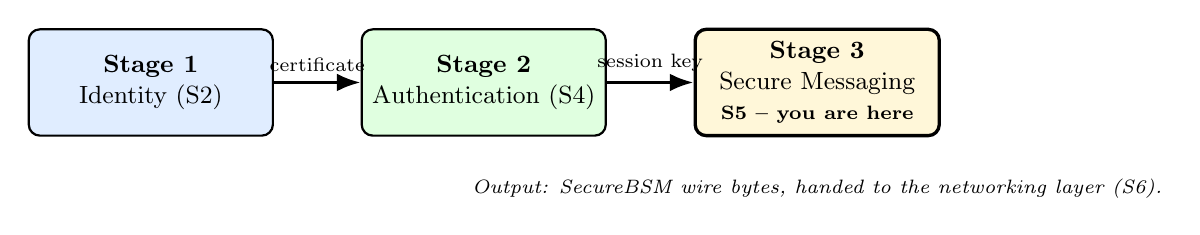
\begin{tikzpicture}[node distance=9mm and 11mm,every node/.style={font=\small},
    stage/.style={draw,rounded corners,minimum width=3.1cm,minimum height=1.35cm,
                  align=center,thick}]
  \node[stage,fill=boxblue]   (id)   {\textbf{Stage 1}\\Identity (S2)};
  \node[stage,fill=green!12,right=of id]   (auth) {\textbf{Stage 2}\\Authentication (S4)};
  \node[stage,fill=boxyellow,very thick,right=of auth] (msg)
       {\textbf{Stage 3}\\Secure Messaging\\\scriptsize \textbf{S5 -- you are here}};
  \draw[-{Latex[length=3mm]},very thick] (id)   -- (auth)
       node[midway,above,font=\scriptsize]{certificate};
  \draw[-{Latex[length=3mm]},very thick] (auth) -- (msg)
       node[midway,above,font=\scriptsize]{session key};
  \node[below=4mm of msg,font=\scriptsize\itshape,align=center]
       {Output: SecureBSM wire bytes, handed to the networking layer (S6).};
\end{tikzpicture}
\end{center}

% =====================================================================
\section{The Theory You Must Study}
% =====================================================================

\subsection{The Basic Safety Message (BSM)}
\textbf{Plain definition.} A BSM is the small data record a vehicle broadcasts:
its speed, heading, position, braking state and so on. In code it is the
\texttt{BasicSafetyMessage} dataclass.

\textbf{Real-life analogy.} A quick spoken status update: ``This is car A, doing
80, heading north-east, not braking, message number 5.''

\textbf{Why it exists.} Other cars need a small, standard, frequently-updated
record of what each nearby vehicle is doing, so they can react to danger.

\textbf{How it works here.} The dataclass carries nine fields:
\texttt{vehicle\_id}, \texttt{speed\_kmh}, \texttt{heading\_deg} (0 = North,
90 = East), \texttt{latitude}, \texttt{longitude}, \texttt{timestamp},
\texttt{sequence\_num}, \texttt{brake\_applied}, and \texttt{acceleration}.
Real V2V broadcasts a BSM about ten times a second; this project sends one per
second --- a deliberate slowdown so a human can watch the dashboard.

\textbf{Security property it relates to.} The BSM is the \emph{thing being
protected}; the rest of S5 is the protection.

\subsection{Sign-then-Encrypt}
\textbf{Plain definition.} ``Sign-then-Encrypt'' means: first create a digital
signature over the \emph{plaintext} message, then encrypt the message
\emph{and} its signature together.

\textbf{Real-life analogy.} You sign a letter by hand, then put the signed letter
inside a sealed, tamper-evident envelope. Anyone who opens the envelope finds a
letter that already carries your signature.

\textbf{Why it exists --- the alternative is worse.} The opposite order,
Encrypt-then-Sign, signs the \emph{ciphertext}. An attacker could then peel that
signature off and glue it onto a \emph{different} ciphertext, because the
signature was never tied to the actual message content. By signing the plaintext
first, the signature is bound to what the message really says. The file's own
docstring states this reasoning explicitly.

\textbf{How it works here.} \texttt{secure\_send} runs: serialize BSM
$\rightarrow$ \texttt{ecdsa\_sign} the BSM bytes $\rightarrow$ glue
\texttt{[length][BSM][signature]} together $\rightarrow$ \texttt{aes\_gcm\_encrypt}
the whole thing.

\textbf{Security property it provides.} \textbf{Non-repudiation} and
\textbf{authentication} (from the signature) wrapped inside
\textbf{confidentiality} and \textbf{integrity} (from the encryption).

\subsection{ECDSA Digital Signatures (recap from S3)}
A digital signature is a value made with a vehicle's \emph{private} key that
anyone with its \emph{public} key can verify. It proves \emph{who} wrote the
message and that it has not changed --- and because only the owner could sign,
they cannot later deny it. S5 simply calls \texttt{ecdsa\_sign} when sending and
\texttt{ecdsa\_verify} when receiving. \emph{Security property:}
\textbf{non-repudiation}, \textbf{authentication}, \textbf{integrity}.

\subsection{AES-256-GCM Authenticated Encryption (recap from S3)}
AES-256-GCM both hides the message (confidentiality) and attaches a 16-byte
authentication tag that detects any change (integrity). S5 calls
\texttt{aes\_gcm\_encrypt} when sending and \texttt{aes\_gcm\_decrypt} when
receiving; a tampered packet makes decryption fail. \emph{Security property:}
\textbf{confidentiality}, \textbf{integrity}.

\subsection{Serialization: JSON and Binary Packing}
\textbf{Plain definition.} \emph{Serialization} turns a structured object into a
flat sequence of bytes. S5 uses \emph{two} kinds:
\begin{itemize}
  \item \textbf{JSON} (JavaScript Object Notation) --- a human-readable text
        format. The BSM fields are turned into JSON text, then into bytes
        (\texttt{to\_bytes} uses \texttt{json.dumps}).
  \item \textbf{Binary struct packing} --- a compact fixed-layout byte format,
        used for the outer \texttt{SecureBSM} envelope.
\end{itemize}

\textbf{Real-life analogy.} JSON is filling in a paper form with words you can
read. Binary packing is a barcode: dense, exact, not human-readable, but quick
and unambiguous for a machine.

\textbf{Why two formats?} The BSM \emph{content} benefits from JSON's
flexibility. The outer envelope needs an exact, compact layout so the receiver
can find each field at a known position --- JSON would be wasteful and harder to
parse byte-precisely.

\textbf{Security property it provides.} None directly --- it is about format.

\subsection{Length-Prefixing and Big-Endian (the \texttt{struct} module)}
\textbf{Plain definition.} \emph{Length-prefixing} means writing a field's length
\emph{just before} the field itself, so the reader knows exactly how many bytes
to take. \emph{Big-endian} is the convention of writing the most significant byte
first (the ``natural'' left-to-right order for numbers).

\textbf{Real-life analogy.} A parcel label that says ``contents: 1742 grams''
before you open it --- you know what to expect. Big-endian is writing the number
``one thousand'' as \texttt{1000}, not \texttt{0001}.

\textbf{Why it exists.} Variable-length fields (the sender's name, the
ciphertext) have no fixed size. Without a length written in front, the receiver
cannot tell where one field ends and the next begins.

\textbf{How it works here.} The \texttt{struct} module packs numbers into bytes:
\texttt{struct.pack(">H", n)} writes \texttt{n} as a 2-byte big-endian unsigned
integer (\texttt{">"} = big-endian, \texttt{"H"} = 2-byte), and
\texttt{struct.pack(">I", n)} writes a 4-byte one (\texttt{"I"} = 4-byte).
\texttt{struct.unpack\_from} reads them back at a given offset.

\textbf{Security property it provides.} None directly --- but \emph{reliable}
framing avoids parsing errors that could be abused.

\subsection{Sequence Numbers and Replay Defence}
\textbf{Plain definition.} A \emph{sequence number} is a counter that increases
by one with every message a vehicle sends. The receiver remembers the last
number it saw and rejects anything not strictly greater.

\textbf{Real-life analogy.} Numbered tickets at a deli counter. If you are
holding ticket 8 and someone hands you ticket 5 again, you know it is an old,
re-used ticket.

\textbf{Why it exists.} A replayed message carries an \emph{old} sequence number.
A suppressed-and-delayed message arrives out of order. Requiring the number to
always increase catches both --- a replayed or stale BSM has a number less than
or equal to the last accepted one.

\textbf{How it works here.} \texttt{secure\_receive} takes a \texttt{last\_seq}
argument; if the new BSM's \texttt{sequence\_num} is \texttt{<= last\_seq} it
raises \texttt{SequenceError}. Combined with the 5-second timestamp window
(\texttt{TimestampValidator}, from S4), an old message has two ways to be caught.

\textbf{Honest note.} \texttt{secure\_receive} also \emph{accepts} a
\texttt{replay\_cache} argument, but --- unlike the handshake --- it does
\emph{not} actually consult the nonce cache in its body. For BSMs the replay
defence is the \emph{sequence number} plus the \emph{timestamp window}, not the
nonce cache. This is worth stating plainly if an examiner asks.

\textbf{Security property it provides.} \textbf{Replay prevention}.

% =====================================================================
\section{Code Walkthrough}
% =====================================================================

\texttt{v2v\_protocol.py} contains: three exceptions, two dataclasses
(\texttt{BasicSafetyMessage}, \texttt{SecureBSM}), the \texttt{MessageLogger}
class, and the two key functions \texttt{secure\_send} and
\texttt{secure\_receive}.

\subsection{The three exceptions}
\begin{lstlisting}[style=py,caption={v2v\_protocol.py --- the messaging exceptions.}]
class TamperError(Exception):
    """Message was modified in transit (AES-GCM tag mismatch or bad sig)."""

class ReplayError(Exception):
    """Duplicate message detected (same nonce or old timestamp)."""

class SequenceError(Exception):
    """Sequence number out of order -- possible message suppression."""
\end{lstlisting}
\textbf{Explanation:} \texttt{TamperError} means the packet failed an integrity
check (the AES-GCM tag or the ECDSA signature). \texttt{SequenceError} means the
sequence number went backwards. \texttt{ReplayError} is defined for completeness.
Naming each makes the dashboard's alert log precise.

\subsection{BasicSafetyMessage --- the plain message}
\begin{lstlisting}[style=py,caption={v2v\_protocol.py --- the BasicSafetyMessage dataclass.}]
@dataclass
class BasicSafetyMessage:
    vehicle_id: str
    speed_kmh: float
    heading_deg: float       # 0 = North, 90 = East
    latitude: float
    longitude: float
    timestamp: float
    sequence_num: int
    brake_applied: bool
    acceleration: float = 0.0

    def to_bytes(self) -> bytes:
        return json.dumps(asdict(self)).encode("utf-8")

    @classmethod
    def from_bytes(cls, data: bytes) -> BasicSafetyMessage:
        return cls(**json.loads(data.decode("utf-8")))
\end{lstlisting}
\textbf{Step by step:}
\begin{enumerate}
  \item The nine fields hold everything one safety broadcast says.
  \item \texttt{to\_bytes}: \texttt{asdict(self)} turns the object into a plain
        dictionary; \texttt{json.dumps} turns that into JSON text;
        \texttt{.encode("utf-8")} turns the text into bytes ready to be signed
        and encrypted.
  \item \texttt{from\_bytes}: the reverse --- decode bytes to text, parse the
        JSON to a dictionary, and build a fresh \texttt{BasicSafetyMessage}.
\end{enumerate}
\textbf{Theory link:} JSON serialization. \emph{Analogy:} filling in the paper
form (\texttt{to\_bytes}) and reading it back (\texttt{from\_bytes}).

\subsection{SecureBSM --- the on-the-wire envelope}
\begin{lstlisting}[style=py,caption={v2v\_protocol.py --- SecureBSM and its binary wire format.}]
@dataclass
class SecureBSM:
    ciphertext: bytes
    nonce: bytes          # 12-byte AES-GCM nonce
    auth_tag: bytes       # 16-byte AES-GCM tag
    sender_id: str
    sequence_num: int

    def to_bytes(self) -> bytes:
        # Wire format:
        # [sid_len:2][sid][seq:4][nonce:12][tag:16][ct_len:4][ciphertext]
        sid = self.sender_id.encode("utf-8")
        parts = [
            struct.pack(">H", len(sid)),
            sid,
            struct.pack(">I", self.sequence_num),
            self.nonce,    # always 12 bytes
            self.auth_tag, # always 16 bytes
            struct.pack(">I", len(self.ciphertext)),
            self.ciphertext,
        ]
        return b"".join(parts)

    @classmethod
    def from_bytes(cls, data: bytes) -> SecureBSM:
        offset = 0
        sid_len = struct.unpack_from(">H", data, offset)[0]; offset += 2
        sender_id = data[offset:offset + sid_len].decode("utf-8"); offset += sid_len
        seq = struct.unpack_from(">I", data, offset)[0]; offset += 4
        nonce = data[offset:offset + 12]; offset += 12
        tag = data[offset:offset + 16]; offset += 16
        ct_len = struct.unpack_from(">I", data, offset)[0]; offset += 4
        ciphertext = data[offset:offset + ct_len]
        return cls(ciphertext, nonce, tag, sender_id, seq)
\end{lstlisting}
\textbf{Step by step (\texttt{to\_bytes}):}
\begin{enumerate}
  \item Encode the sender's name to bytes.
  \item Write its length as a 2-byte big-endian number (\texttt{">H"}), then the
        name itself --- length-prefixing in action.
  \item Write the sequence number as a 4-byte big-endian number (\texttt{">I"}).
  \item Append the nonce (always 12 bytes) and the auth tag (always 16 bytes) ---
        no length prefix needed because their sizes are fixed.
  \item Write the ciphertext length (4 bytes), then the ciphertext.
  \item \texttt{b"".join(parts)} concatenates everything into one byte string.
\end{enumerate}
\textbf{\texttt{from\_bytes}} walks an \texttt{offset} cursor through the bytes,
reading each field at its known position --- the exact reverse of
\texttt{to\_bytes}. \textbf{Theory link:} binary serialization, length-prefixing,
big-endian. \emph{Analogy:} packing a parcel with a clear packing list, then
unpacking it item by item.

\subsection{MessageLogger --- the record keeper}
\textbf{Purpose:} keep a rolling record of sent/received messages and security
alerts, plus counters, for the dashboard (S7) to display.
\begin{lstlisting}[style=py,caption={v2v\_protocol.py --- MessageLogger (key parts).}]
class MessageLogger:
    def __init__(self, max_messages: int = 50) -> None:
        self._messages: list[dict] = []
        self._alerts: list[dict] = []
        self._max = max_messages
        self.total_sent = 0
        self.total_received = 0
        self.tamper_blocked = 0
        self.replay_blocked = 0

    def log_sent(self, bsm): ...        # +1 total_sent, append a SENT entry
    def log_received(self, bsm, security_props): ...   # +1 total_received
    def log_alert(self, alert_type, details):
        if alert_type == "TAMPER":  self.tamper_blocked += 1
        elif alert_type == "REPLAY": self.replay_blocked += 1
        self._alerts.append({...})
\end{lstlisting}
\textbf{Step by step:}
\begin{enumerate}
  \item It holds two rolling lists --- \texttt{\_messages} and \texttt{\_alerts}
        --- and four counters.
  \item \texttt{log\_sent} / \texttt{log\_received} append a small dictionary
        describing the message and trim the list to \texttt{max\_messages}
        (default 50) so memory does not grow forever.
  \item \texttt{log\_alert} bumps \texttt{tamper\_blocked} or
        \texttt{replay\_blocked} depending on the alert type, and records the
        alert with a timestamp.
  \item \texttt{get\_recent}, \texttt{get\_alerts} and \texttt{clear\_alerts} are
        read/clear helpers the dashboard calls.
\end{enumerate}
\textbf{Theory link:} this is \emph{observability}, not a defence --- it lets a
human \emph{see} that the defences fired. \emph{Analogy:} the CCTV logbook at a
building's front desk.

\subsection{secure\_send() --- Sign-then-Encrypt}
\begin{lstlisting}[style=py,caption={v2v\_protocol.py --- secure\_send: the sending pipeline.}]
def secure_send(bsm, session_key, signing_key, logger) -> bytes:
    # Step 1: serialize BSM to bytes
    bsm_bytes = bsm.to_bytes()
    # Step 2: sign the PLAINTEXT (Sign-then-Encrypt)
    signature = ecdsa_sign(signing_key, bsm_bytes)
    # Step 3: combine with a 4-byte length prefix
    payload = struct.pack(">I", len(bsm_bytes)) + bsm_bytes + signature
    # Step 4: AES-256-GCM encrypt -- confidentiality + integrity
    ciphertext, nonce, auth_tag = aes_gcm_encrypt(session_key, payload)
    # Step 5: wrap in SecureBSM and return wire bytes
    secure = SecureBSM(ciphertext, nonce, auth_tag, bsm.vehicle_id, bsm.sequence_num)
    logger.log_sent(bsm)
    return secure.to_bytes()
\end{lstlisting}
\textbf{Step by step:}
\begin{enumerate}
  \item \textbf{Serialize} --- turn the BSM into JSON bytes.
  \item \textbf{Sign the plaintext} --- \texttt{ecdsa\_sign} produces a signature
        over those exact bytes. Doing this \emph{before} encryption is the whole
        point of Sign-then-Encrypt.
  \item \textbf{Combine} --- glue \texttt{[4-byte length][BSM bytes][signature]}
        so the receiver can later split them apart again.
  \item \textbf{Encrypt} --- \texttt{aes\_gcm\_encrypt} encrypts the combined
        payload, returning ciphertext, a fresh nonce, and a 16-byte tag.
  \item \textbf{Wrap} --- build a \texttt{SecureBSM}, log the send, and return
        \texttt{secure.to\_bytes()} --- the final wire bytes.
\end{enumerate}
\textbf{Arguments:} \texttt{bsm} (the message), \texttt{session\_key} (32-byte
AES key from the handshake), \texttt{signing\_key} (this vehicle's ECDSA private
key), \texttt{logger}. \textbf{Returns:} wire-format \texttt{bytes}.
\textbf{Theory link:} Sign-then-Encrypt; ECDSA; AES-GCM; length-prefixing.

\subsection{secure\_receive() --- Decrypt-then-Verify}
\begin{lstlisting}[style=py,caption={v2v\_protocol.py --- secure\_receive: the receiving pipeline.}]
def secure_receive(data, session_key, peer_verify_key, replay_cache,
                   timestamp_validator, logger, last_seq=None):
    # Step 1: parse SecureBSM from raw bytes
    secure = SecureBSM.from_bytes(data)
    # Step 2: AES-GCM decrypt -- 1 changed bit -> failure
    try:
        plaintext = aes_gcm_decrypt(session_key, secure.ciphertext,
                                    secure.nonce, secure.auth_tag)
    except DecryptionError as exc:
        logger.log_alert("TAMPER", f"AES-GCM decryption failed: {exc}")
        raise TamperError("Message tampered -- AES-GCM auth tag mismatch") from exc
    # Step 3: split plaintext into BSM bytes + signature
    bsm_len = struct.unpack_from(">I", plaintext, 0)[0]
    bsm_bytes = plaintext[4:4 + bsm_len]
    signature = plaintext[4 + bsm_len:]
    # Step 4: verify the ECDSA signature
    if not ecdsa_verify(peer_verify_key, bsm_bytes, signature):
        logger.log_alert("TAMPER", "ECDSA signature verification failed")
        raise TamperError("Invalid ECDSA signature -- message not authentic")
    # Step 5: parse BSM, check sequence number, validate timestamp
    bsm = BasicSafetyMessage.from_bytes(bsm_bytes)
    if last_seq is not None and bsm.sequence_num <= last_seq:
        logger.log_alert("REPLAY", f"Seq {bsm.sequence_num} <= last {last_seq}")
        raise SequenceError(f"Sequence {bsm.sequence_num} not greater than {last_seq}")
    timestamp_validator.validate(bsm.timestamp)
    logger.log_received(bsm, {"authenticated": True, "encrypted": True,
                              "integrity_verified": True, "replay_protected": True})
    return bsm
\end{lstlisting}
\textbf{Step by step:}
\begin{enumerate}
  \item \textbf{Parse} the raw bytes back into a \texttt{SecureBSM}
        (\texttt{from\_bytes}).
  \item \textbf{Decrypt} with \texttt{aes\_gcm\_decrypt}. If a single bit was
        changed, the tag check fails: the code catches \texttt{DecryptionError},
        logs a \texttt{TAMPER} alert, and raises \texttt{TamperError}.
  \item \textbf{Split} the decrypted payload using the 4-byte length prefix into
        the BSM bytes and the signature.
  \item \textbf{Verify the signature} with \texttt{ecdsa\_verify} against the
        peer's public key. If it fails, log a \texttt{TAMPER} alert and raise
        \texttt{TamperError}. This is the second integrity check --- and the one
        that gives \textbf{non-repudiation}.
  \item \textbf{Parse and validate.} Rebuild the BSM. If the sequence number is
        not greater than \texttt{last\_seq}, raise \texttt{SequenceError}
        (replay). Then \texttt{timestamp\_validator.validate} rejects a stale
        timestamp. If all pass, log a successful receive and return the BSM.
\end{enumerate}
\textbf{Arguments / return / exceptions:} returns the verified
\texttt{BasicSafetyMessage}; raises \texttt{TamperError} (bad tag or bad
signature), \texttt{SequenceError} (replay), or \texttt{StaleMessageError}
(stale timestamp). \textbf{Honest note:} the \texttt{replay\_cache} parameter is
accepted but not used in the body --- BSM replay defence here is the sequence
number and timestamp. \textbf{Theory link:} AES-GCM integrity, ECDSA
authentication, sequence/timestamp replay defence.

\subsection{The demo block}
The \texttt{if \_\_name\_\_ == "\_\_main\_\_"} block builds a session key, creates
a BSM, calls \texttt{secure\_send} then \texttt{secure\_receive} (showing a clean
round-trip), then flips a byte and shows the tampered message is rejected with a
\texttt{TamperError}. We run it next.

% =====================================================================
\section{Hands-On / Practical}
% =====================================================================

\subsection{Run the messaging protocol by itself}
\texttt{v2v\_protocol.py} needs no certificates and no network --- run it directly:
\begin{lstlisting}[style=term]
python protocol\v2v_protocol.py
\end{lstlisting}

\noindent\textbf{Expected output (sample):}
\begin{lstlisting}[style=term]
=== V2V MESSAGE PROTOCOL DEMO ===

Session key: 4a9c1f0b7e2d6688c3a5...

[SEND] BSM: speed=72.5 km/h, seq=1
[WIRE] 338 bytes on the wire (encrypted)
[RECV] BSM: speed=72.5 km/h, seq=1
[OK] All security checks passed!

--- TAMPER TEST ---
[OK] Tampered message REJECTED: Message tampered -- AES-GCM auth tag mismatch

Stats: sent=1, recv=1, tamper_blocked=1
\end{lstlisting}

\subsection{What the output lines mean}
\begin{itemize}
  \item \texttt{Session key} --- a 32-byte key (here simulated, normally from the
        S4 handshake).
  \item \texttt{[SEND]} --- the plain BSM before protection.
  \item \texttt{[WIRE] 338 bytes} --- the size of the signed-and-encrypted
        packet; the exact number depends on the JSON content.
  \item \texttt{[RECV] ... [OK]} --- decryption, signature check, sequence and
        timestamp checks all passed; the message came back identical.
  \item \texttt{Tampered message REJECTED} --- one flipped byte made the AES-GCM
        tag mismatch, so \texttt{secure\_receive} raised \texttt{TamperError}.
  \item \texttt{tamper\_blocked=1} --- the \texttt{MessageLogger} counted the
        blocked attack.
\end{itemize}

\subsection{Try This Yourself (mini-experiment)}
In the demo's tamper test, the line \texttt{tampered[len(tampered) // 2] \^{}= 0xFF}
flips one byte in the \emph{middle} of the packet. Change it to flip a byte near
the \emph{start} instead:
\begin{lstlisting}[style=term]
tampered[0] ^= 0xFF        # flip the very first byte
\end{lstlisting}
\textbf{Predict before you run.} Byte~0 is part of the \texttt{sid\_len} field
(the 2-byte sender-name length). Corrupting it makes \texttt{SecureBSM.from\_bytes}
read a wrong length and the unpacking fails \emph{before} decryption even starts
--- so instead of a clean \texttt{TamperError} you may see a different exception
(for example a \texttt{struct} or decode error), caught by the demo's general
\texttt{except Exception} branch as ``Message rejected''. Lesson: tampering is
caught \emph{somewhere} on every path --- but exactly which check fires depends
on \emph{which} bytes you damage.

% =====================================================================
\section{Attack Relevance}
% =====================================================================

S5 is the layer that defends \emph{every individual safety message}. It is
exercised directly by \texttt{attacks/tamper\_attack.py} and
\texttt{attacks/replay\_attack.py}.

\begin{table}[h]
\centering
\small
\begin{tabular}{@{}p{2.5cm} p{6.1cm} p{4.9cm}@{}}
\toprule
\textbf{Attack} & \textbf{How S5 stops it} & \textbf{The mechanism}\\
\midrule
Tamper & A changed byte breaks the AES-GCM tag; a forged body breaks the ECDSA
signature. & \texttt{aes\_gcm\_decrypt} / \texttt{ecdsa\_verify} $\to$
\texttt{TamperError}.\\
Replay & A re-sent BSM carries an old sequence number or a stale timestamp. &
sequence check $\to$ \texttt{SequenceError}; \texttt{TimestampValidator} $\to$
\texttt{StaleMessageError}.\\
Eavesdrop & The BSM travels as AES-256 ciphertext; unreadable without the
session key. & \texttt{aes\_gcm\_encrypt} in \texttt{secure\_send}.\\
Forgery / denial & The plaintext signature ties the message to its true author,
who cannot deny it. & ECDSA signature (non-repudiation).\\
\bottomrule
\end{tabular}
\caption{S5 defends confidentiality, integrity, replay prevention and non-repudiation per message.}
\end{table}

\noindent\textbf{Why Sign-then-Encrypt matters for the attacker.} Because the
signature covers the \emph{plaintext}, an attacker cannot take a valid signature
from one message and re-attach it to a different one --- the signature would not
match the new content. And because the signature is \emph{inside} the encrypted
envelope, the attacker cannot even read or strip it without the session key.
\textbf{Honest scope note:} S5 protects each message, but it relies on a correct
session key from S4; if the handshake were skipped or compromised, S5 alone could
not help.

% =====================================================================
\section{Illustrations}
% =====================================================================

\subsection{Diagram 1 --- the Sign-then-Encrypt pipeline}
\begin{center}
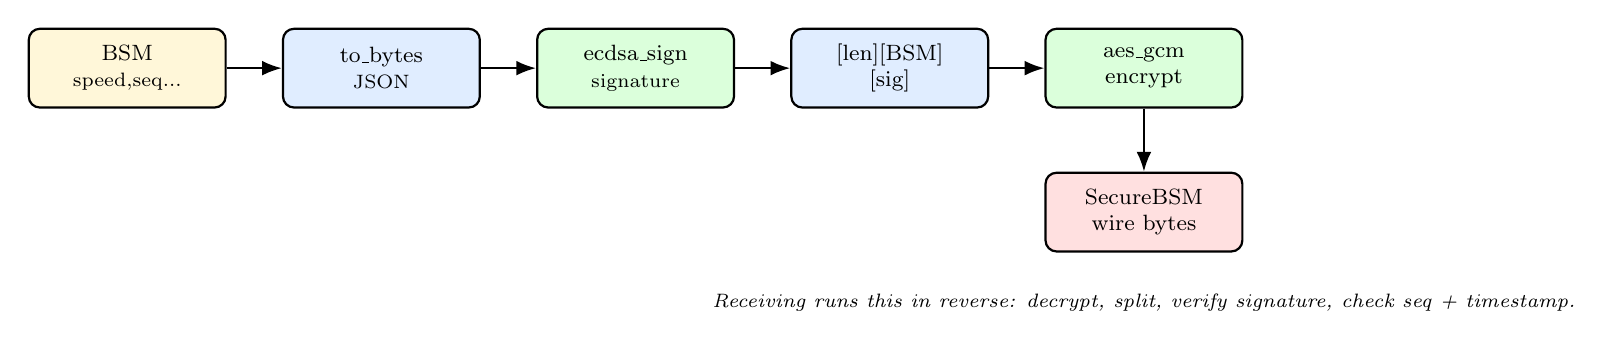
\begin{tikzpicture}[font=\footnotesize,node distance=5mm,
   box/.style={draw,thick,rounded corners,minimum width=2.5cm,minimum height=1.0cm,
               align=center}]
  \node[box,fill=boxyellow] (bsm) {BSM\\\scriptsize speed,seq...};
  \node[box,fill=boxblue,right=7mm of bsm] (json) {to\_bytes\\\scriptsize JSON};
  \node[box,fill=green!14,right=7mm of json] (sign) {ecdsa\_sign\\\scriptsize signature};
  \node[box,fill=boxblue,right=7mm of sign] (comb) {[len][BSM]\\{[sig]}};
  \node[box,fill=green!14,right=7mm of comb] (enc) {aes\_gcm\\encrypt};
  \node[box,fill=red!12,below=8mm of enc] (wire) {SecureBSM\\wire bytes};
  \draw[-{Latex[length=2.5mm]},thick] (bsm) -- (json);
  \draw[-{Latex[length=2.5mm]},thick] (json) -- (sign);
  \draw[-{Latex[length=2.5mm]},thick] (sign) -- (comb);
  \draw[-{Latex[length=2.5mm]},thick] (comb) -- (enc);
  \draw[-{Latex[length=2.5mm]},thick] (enc) -- (wire);
  \node[below=4mm of wire,font=\scriptsize\itshape]
       {Receiving runs this in reverse: decrypt, split, verify signature, check seq + timestamp.};
\end{tikzpicture}
\end{center}

\subsection{Diagram 2 --- the SecureBSM wire format}
\begin{center}
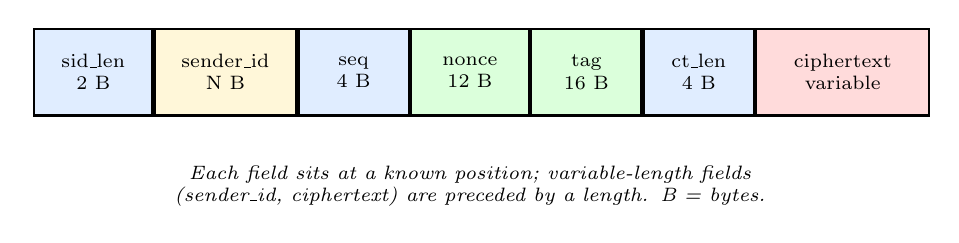
\begin{tikzpicture}[font=\scriptsize,
   f/.style={draw,thick,minimum height=1.1cm,align=center}]
  \node[f,fill=boxblue,minimum width=1.5cm]              (a) {sid\_len\\2 B};
  \node[f,fill=boxyellow,minimum width=1.8cm,right=0 of a] (b) {sender\_id\\N B};
  \node[f,fill=boxblue,minimum width=1.4cm,right=0 of b] (c) {seq\\4 B};
  \node[f,fill=green!14,minimum width=1.5cm,right=0 of c] (d) {nonce\\12 B};
  \node[f,fill=green!14,minimum width=1.4cm,right=0 of d] (e) {tag\\16 B};
  \node[f,fill=boxblue,minimum width=1.4cm,right=0 of e] (g) {ct\_len\\4 B};
  \node[f,fill=red!14,minimum width=2.2cm,right=0 of g] (h) {ciphertext\\variable};
  \node[below=5mm of d,font=\scriptsize\itshape,align=center,text width=11cm]
       {Each field sits at a known position; variable-length fields
        (sender\_id, ciphertext) are preceded by a length. B = bytes.};
\end{tikzpicture}
\end{center}

% =====================================================================
\section{Presentation Pack}
% =====================================================================

\subsection{Slide Outline}

\textbf{Slide 1 --- The Job of S5.}
\begin{itemize}
  \item The handshake gave us a shared key --- now we can talk.
  \item A BSM is a tiny ``speed, heading, braking'' status message.
  \item S5 turns a plain BSM into a safe packet, and back again.
  \item One file: \texttt{v2v\_protocol.py}.
\end{itemize}

\textbf{Slide 2 --- Sign-then-Encrypt.}
\begin{itemize}
  \item First sign the plaintext, then encrypt message + signature together.
  \item Sign first $\to$ the signature is tied to the real content.
  \item Encrypt-then-Sign would let an attacker swap signatures.
  \item Result: a signed letter inside a sealed envelope.
\end{itemize}

\textbf{Slide 3 --- The SecureBSM Wire Format.}
\begin{itemize}
  \item An exact byte layout: lengths, ids, nonce, tag, ciphertext.
  \item Length-prefixing tells the receiver where each field ends.
  \item Big-endian packing via Python's \texttt{struct} module.
  \item Fixed-size fields (nonce 12 B, tag 16 B) need no length.
\end{itemize}

\textbf{Slide 4 --- Receiving: Four Checks.}
\begin{itemize}
  \item Decrypt --- AES-GCM tag catches any tampering.
  \item Verify signature --- ECDSA proves the true author.
  \item Sequence number --- must always increase (anti-replay).
  \item Timestamp --- must be within 5 seconds (anti-replay).
\end{itemize}

\textbf{Slide 5 --- What S5 Guarantees Per Message.}
\begin{itemize}
  \item Confidentiality + integrity (AES-256-GCM).
  \item Authentication + non-repudiation (ECDSA signature).
  \item Replay prevention (sequence + timestamp).
  \item A single flipped bit $\to$ \texttt{TamperError}.
\end{itemize}

\subsection{Speaker Talking Points (about 30--60 seconds each)}

\textbf{Slide 1.} ``After the handshake in the previous section, our two cars
share a secret key. Now they can actually talk. What they say are Basic Safety
Messages --- tiny records of speed, heading, position and braking. Section five
is the file that protects each of those messages. It takes a plain BSM, wraps it
in security, produces the exact bytes that go on the wire, and on the other side
unwraps it and checks it. It is all in one file, v2v\_protocol.py.''

\textbf{Slide 2.} ``The protection recipe is called Sign-then-Encrypt. We first
make a digital signature over the plain message, and only then encrypt the
message and its signature together. Order matters. If we encrypted first and
signed the ciphertext, an attacker could peel that signature off and stick it on
a different ciphertext, because the signature was never connected to the real
words. By signing the plaintext first, the signature is glued to what the
message actually says. Picture signing a letter by hand, then sealing it in a
tamper-evident envelope.''

\textbf{Slide 3.} ``A network only carries a flat stream of bytes, so we need an
exact layout --- the wire format. The SecureBSM packet is: a two-byte length,
then the sender's name, then a four-byte sequence number, then the twelve-byte
nonce, the sixteen-byte tag, a four-byte ciphertext length, and finally the
ciphertext. The trick is length-prefixing: before any variable-size field we
write its length, so the receiver knows exactly where it ends. We build this with
Python's struct module in big-endian order.''

\textbf{Slide 4.} ``Receiving is the reverse, and it is four checks in a row.
First we decrypt --- and AES-GCM's tag means any tampering makes decryption fail
outright. Second we verify the ECDSA signature, which proves the message really
came from the claimed car. Third we check the sequence number is larger than the
last one we accepted --- an old or replayed message has an old number. Fourth we
check the timestamp is fresh, within five seconds. Only a message that passes all
four is delivered.''

\textbf{Slide 5.} ``So per message, S5 delivers four security properties at once.
AES-256-GCM gives confidentiality and integrity. The ECDSA signature gives
authentication and non-repudiation --- the sender cannot deny it. And the
sequence number plus timestamp give replay prevention. The demo proves it: flip
a single bit anywhere in the packet and the receiver throws a TamperError instead
of trusting the message.''

\subsection{Live-Demo Script}
\begin{enumerate}
  \item \textbf{Run the demo.} Execute \texttt{python
        protocol\textbackslash v2v\_protocol.py}.
  \item \textbf{Point at the round-trip.} \texttt{[SEND]} then \texttt{[RECV]}
        with the same speed and sequence number --- ``protected and recovered
        perfectly.''
  \item \textbf{Point at the wire size.} \texttt{[WIRE] 338 bytes} --- ``that is
        the signed, encrypted packet.''
  \item \textbf{Point at the tamper test.} \texttt{Tampered message REJECTED} ---
        ``one byte changed, the whole message refused.''
  \item \textbf{Optional break-it.} Change the flipped index to \texttt{0} (see
        the mini-experiment) and show a different rejection path.
\end{enumerate}

\subsection{Examiner Q\&A}
\begin{enumerate}
  \item \textbf{Q: What is a BSM and what fields does it carry here?}\\
        A: A Basic Safety Message. The \texttt{BasicSafetyMessage} dataclass
        carries vehicle id, speed, heading, latitude, longitude, timestamp,
        sequence number, brake flag and acceleration.
  \item \textbf{Q: What is Sign-then-Encrypt and why not the reverse?}\\
        A: Sign the plaintext first, then encrypt message + signature. The
        reverse (signing the ciphertext) would let an attacker move a signature
        onto a different ciphertext, since it would not be bound to content.
  \item \textbf{Q: Describe the SecureBSM wire format.}\\
        A: \texttt{[sid\_len:2][sender\_id][seq:4][nonce:12][tag:16][ct\_len:4]
        [ciphertext]} --- length-prefixed, big-endian, built with \texttt{struct}.
  \item \textbf{Q: Why length-prefix the variable fields?}\\
        A: The sender name and ciphertext have no fixed size; writing the length
        first tells the receiver exactly how many bytes to read.
  \item \textbf{Q: How does \texttt{secure\_receive} detect a tampered message?}\\
        A: Two ways: \texttt{aes\_gcm\_decrypt} fails if the ciphertext/nonce/tag
        changed (\texttt{DecryptionError} $\to$ \texttt{TamperError}), and
        \texttt{ecdsa\_verify} fails if the body does not match the signature.
  \item \textbf{Q: How does S5 stop replay?}\\
        A: The sequence number must be strictly greater than the last accepted
        one (\texttt{SequenceError} otherwise), and the timestamp must be within
        5 seconds.
  \item \textbf{Q: The \texttt{replay\_cache} argument --- is it used?}\\
        A: It is accepted by \texttt{secure\_receive} but not consulted in the
        body. BSM replay defence is the sequence number plus the timestamp; the
        nonce cache is used by the handshake, not here.
  \item \textbf{Q: What does \texttt{MessageLogger} contribute to security?}\\
        A: Nothing directly --- it is observability. It records sent/received
        messages and counts blocked tamper/replay attempts so the dashboard can
        display them.
\end{enumerate}

% =====================================================================
\section{Glossary}
% =====================================================================
\begin{description}[style=nextline,leftmargin=0pt]
  \item[BSM] Basic Safety Message: the small status broadcast of a vehicle.
  \item[BasicSafetyMessage] The dataclass holding the BSM fields.
  \item[SecureBSM] The signed-and-encrypted on-the-wire form of a BSM.
  \item[Sign-then-Encrypt] Sign the plaintext, then encrypt message + signature.
  \item[Plaintext] The original readable message before encryption.
  \item[Ciphertext] The scrambled output of encryption.
  \item[Wire format] The exact byte layout of a packet sent over a network.
  \item[Serialization] Turning an object into a flat sequence of bytes.
  \item[JSON] A human-readable text format for structured data.
  \item[struct module] Python module that packs/unpacks numbers into bytes.
  \item[Length-prefixing] Writing a field's length just before the field.
  \item[Big-endian] Byte order with the most significant byte first.
  \item[Nonce] A one-time 12-byte value for AES-GCM encryption.
  \item[Authentication tag] The 16-byte AES-GCM value that detects tampering.
  \item[ECDSA] Elliptic Curve Digital Signature Algorithm.
  \item[Digital signature] A private-key value provable with the public key.
  \item[Sequence number] A per-sender counter that must always increase.
  \item[Timestamp] The recorded creation time, checked for freshness.
  \item[Session key] The shared 32-byte AES key from the handshake.
  \item[TamperError] Exception meaning a packet failed an integrity check.
  \item[SequenceError] Exception meaning the sequence number went backwards.
  \item[MessageLogger] Class that records messages and alerts for the dashboard.
  \item[Non-repudiation] A sender cannot later deny having sent a message.
  \item[Confidentiality] Only the intended recipient can read the message.
  \item[Integrity] Any change to the message is detected.
\end{description}

% =====================================================================
\section{References and Further Study}
% =====================================================================
\begin{itemize}
  \item \textbf{Python struct module documentation} ---
        \url{https://docs.python.org/3/library/struct.html}\\
        Read for: the format codes \texttt{">H"} and \texttt{">I"} used in the
        wire format.
  \item \textbf{Python json module documentation} ---
        \url{https://docs.python.org/3/library/json.html}\\
        Read for: \texttt{json.dumps} / \texttt{json.loads} used by the BSM.
  \item \textbf{Python dataclasses documentation} ---
        \url{https://docs.python.org/3/library/dataclasses.html}\\
        Read for: how \texttt{BasicSafetyMessage} and \texttt{SecureBSM} work.
  \item \textbf{SAE J2735 (Basic Safety Message standard)} ---
        \url{https://www.sae.org/standards/content/j2735_202309/}\\
        Read for: the real-world BSM this project is inspired by.
  \item \textbf{Authenticated encryption (Wikipedia)} ---
        \url{https://en.wikipedia.org/wiki/Authenticated_encryption}\\
        Read for: why AES-GCM gives confidentiality and integrity together.
  \item \textbf{Sign-then-encrypt discussion (Cryptography Stack Exchange)} ---
        \url{https://crypto.stackexchange.com/questions/5458/should-we-sign-then-encrypt-or-encrypt-then-sign}\\
        Read for: the trade-offs between signing and encrypting order.
  \item \textbf{Endianness (Wikipedia)} ---
        \url{https://en.wikipedia.org/wiki/Endianness}\\
        Read for: what big-endian byte order means.
  \item \textbf{Digital signature (Wikipedia)} ---
        \url{https://en.wikipedia.org/wiki/Digital_signature}\\
        Read for: authentication, integrity and non-repudiation.
  \item \textbf{Python cryptography --- AEAD docs} ---
        \url{https://cryptography.io/en/latest/hazmat/primitives/aead/}\\
        Read for: the AES-GCM functions S5 calls.
  \item \textbf{Replay attack (Wikipedia)} ---
        \url{https://en.wikipedia.org/wiki/Replay_attack}\\
        Read for: why sequence numbers and timestamps defeat replay.
\end{itemize}

\vfill
\begin{center}\footnotesize\itshape
End of Section S5. Next: S6 --- the Vehicle Node and TCP networking that carries
these SecureBSM bytes.
\end{center}



% ===================== 06-vehicle-node-networking.tex =====================
\chapter{S6 --- The Vehicle Node and TCP Networking}

\section{Title and ``What You'll Learn''}
% =====================================================================

\subsection*{Section Title}
\textbf{S6 --- The Vehicle Node: the program you actually run, which connects two
cars over a real network and drives the whole security pipeline end to end.}

\subsection*{Plain-English Summary (read this first)}
Everything so far --- certificates, crypto, the handshake, the message protocol
--- has been a \emph{library}. Section~S6 is the \textbf{program}. One file,
\texttt{vehicle\_node.py}, is launched once per car. One car acts as the
\textbf{server} (it waits for a connection); the other acts as the
\textbf{client} (it dials in). They make a real network connection using
\textbf{TCP}, run the 4-step handshake over it, and then continuously send and
receive encrypted safety messages --- one per second --- using background
\textbf{threads}. S6 is the conductor that calls S2, S3, S4 and S5 in the right
order.

\subsection*{Learning Outcomes}
After studying this section you will be able to:
\begin{itemize}
  \item Explain what \textbf{TCP} and a \textbf{socket} are.
  \item Explain the \textbf{message-framing} problem and how a 4-byte length
        header solves it.
  \item Explain the difference between the \textbf{server} and \textbf{client}
        roles.
  \item Explain why \textbf{threads} are needed and what a \emph{daemon} thread is.
  \item Explain \textbf{connection retries} with exponential backoff.
  \item Walk through every function and method of \texttt{vehicle\_node.py}.
  \item Launch two vehicle nodes, read their logs, and explain how the receive
        loop reacts to an attack.
\end{itemize}

% =====================================================================
\section{Where This Fits}
% =====================================================================

S6 is not one stage of the pipeline --- it is the \emph{frame around all three
stages}. It loads the identity files from S2, builds the \texttt{AuthProtocol}
of S4 (which rests on the crypto of S3), runs the handshake, and then repeatedly
calls the \texttt{secure\_send} / \texttt{secure\_receive} of S5. It also starts
the dashboard of S7. In short: S6 is the integration layer.

\begin{center}
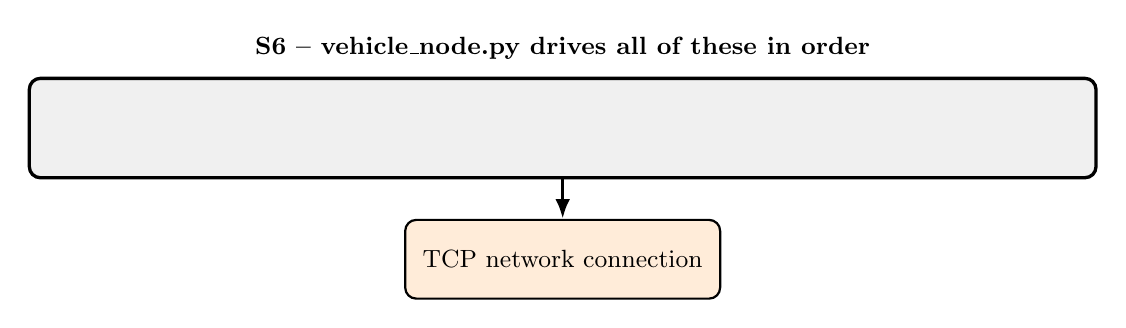
\begin{tikzpicture}[font=\small,node distance=6mm and 8mm,
   st/.style={draw,rounded corners,minimum width=2.7cm,minimum height=1.0cm,
              align=center,thick}]
  \node[st,fill=boxblue]   (id)   {Identity\\\scriptsize S2};
  \node[st,fill=red!12,right=of id]   (cr) {Crypto\\\scriptsize S3};
  \node[st,fill=green!12,right=of cr] (au) {Handshake\\\scriptsize S4};
  \node[st,fill=boxyellow,right=of au] (ms) {Messaging\\\scriptsize S5};
  \node[draw,very thick,rounded corners,fill=gray!12,fit=(id)(cr)(au)(ms)] (box) {};
  \node[above=1mm of box,font=\small\bfseries] {S6 -- vehicle\_node.py drives all of these in order};
  \node[below=5mm of box,st,fill=orange!15,minimum width=4cm] (net) {TCP network connection};
  \draw[-{Latex[length=2.5mm]},very thick] (box) -- (net);
\end{tikzpicture}
\end{center}

% =====================================================================
\section{The Theory You Must Study}
% =====================================================================

\subsection{TCP and Sockets}
\textbf{Plain definition.} \textbf{TCP} (Transmission Control Protocol) is a way
for two programs to send data to each other reliably and in order across a
network. A \textbf{socket} is the software ``end point'' of a connection --- the
object a program reads from and writes to, like the handset of a telephone.

\textbf{Real-life analogy.} A telephone call. TCP is the phone system that makes
sure your words arrive, in order, with nothing dropped. The socket is the handset
in your hand.

\textbf{Why it exists.} The two vehicles run as separate programs (possibly on
separate laptops). They need a dependable channel: TCP guarantees that bytes
arrive complete and in the order they were sent --- something a raw network does
not promise.

\textbf{How it works here.} The code uses Python's \texttt{socket} module.
\texttt{socket.socket(AF\_INET, SOCK\_STREAM)} creates a TCP socket. The server
\emph{binds} to a port and \emph{listens}; the client \emph{connects}.

\textbf{Security property it provides.} None. \textbf{This is important:} TCP is
\emph{not} encrypted. The radio/network is still untrusted. All the security
comes from the \emph{payload} (the SecureBSM of S5), not from TCP.

\subsection{The Message-Framing Problem}
\textbf{Plain definition.} TCP delivers a \emph{byte stream} --- an unbroken flow
of bytes with \emph{no markers} showing where one message ends and the next
begins. \emph{Framing} is the technique of adding those markers.

\textbf{Real-life analogy.} Imagine a friend reading you a long list of phone
numbers with no pauses: ``07700900461077009005...''. Without a gap or a stated
length, you cannot tell where one number ends. Framing is agreeing in advance:
``each number is exactly 11 digits''.

\textbf{Why it exists.} A single \texttt{recv()} call might return half a message,
or two messages stuck together. Without framing the receiver cannot reliably
split the stream into messages.

\textbf{How it works here.} The project uses \textbf{length-prefix framing}.
Before every message, \texttt{send\_framed} writes a 4-byte big-endian number
saying how long the message is. \texttt{recv\_framed} first reads exactly those
4 bytes, learns the length, then reads exactly that many more bytes.

\textbf{Security property it provides.} None directly --- but reliable framing
prevents parsing confusion that an attacker might otherwise exploit.

\subsection{Server and Client Roles}
\textbf{Plain definition.} The \textbf{server} is the side that waits to be
contacted (it \emph{listens} on a port). The \textbf{client} is the side that
starts the conversation (it \emph{connects} to the server's address).

\textbf{Real-life analogy.} A shop and a customer. The shop opens its doors and
waits (server). The customer walks in (client). After that, both can talk freely.

\textbf{Why it exists.} \emph{Someone} has to be reachable first. One side must
be ready and waiting before the other can connect.

\textbf{How it works here.} A vehicle started \emph{without} \texttt{--peer-host}
is a pure server: it just waits. A vehicle started \emph{with}
\texttt{--peer-host} also starts its own server thread \emph{and} then connects
to the peer as a client. In the handshake, the client becomes the
\emph{initiator} (sends HELLO first) and the server becomes the
\emph{responder}.

\textbf{Security property it provides.} None --- it is about connection setup.

\subsection{Threads and Concurrency}
\textbf{Plain definition.} A \textbf{thread} is a separate line of execution
inside the same program, so the program can do more than one thing at a time.

\textbf{Real-life analogy.} One person can only talk \emph{or} listen at once. To
have a real conversation you need two people: one always ready to speak, one
always ready to listen. Threads give the program that second ``person''.

\textbf{Why it exists.} Sending a BSM every second and receiving BSMs at any time
must happen \emph{simultaneously}. If the program were stuck waiting to receive,
it could never send, and vice versa. So the node runs a \emph{send loop} in one
thread and a \emph{receive loop} in another.

\textbf{How it works here.} \texttt{threading.Thread(target=..., daemon=True)}
creates a thread. A \textbf{daemon} thread is one that does not keep the program
alive on its own --- when the main program exits, daemon threads stop too. The
node uses daemon threads for the server-accept loop, the send loop, the receive
loop and the dashboard.

\textbf{Security property it provides.} None --- it is about doing two jobs at once.

\subsection{Connection Retries and Exponential Backoff}
\textbf{Plain definition.} If the client cannot connect (the server is not ready
yet), it tries again. \emph{Exponential backoff} means waiting a bit longer
before each retry.

\textbf{Real-life analogy.} Phoning a friend who is busy: you call, wait a
minute, call again, wait two minutes, call again --- you do not redial
non-stop.

\textbf{Why it exists.} When two laptops start at slightly different times, the
client may dial before the server is listening. Retrying with growing pauses
gives the server time to come up without hammering the network.

\textbf{How it works here.} \texttt{connect\_to\_peer} tries up to five times; on
failure it sleeps \texttt{2 * attempt} seconds (2\,s, 4\,s, 6\,s, 8\,s) before
the next try.

\textbf{Security property it provides.} None --- it is about robustness.

% =====================================================================
\section{Code Walkthrough}
% =====================================================================

\subsection{The TCP framing helpers}
\begin{lstlisting}[style=py,caption={vehicle\_node.py --- length-prefix framing helpers.}]
def send_framed(sock: socket.socket, data: bytes) -> None:
    """Send *data* prefixed with a 4-byte length header."""
    sock.sendall(struct.pack(">I", len(data)) + data)

def _recv_exactly(sock: socket.socket, n: int) -> bytes:
    """Block until exactly *n* bytes have been received."""
    buf = b""
    while len(buf) < n:
        chunk = sock.recv(n - len(buf))
        if not chunk:
            raise ConnectionError("Connection closed by peer")
        buf += chunk
    return buf

def recv_framed(sock: socket.socket) -> bytes:
    """Receive a length-prefixed message."""
    header = _recv_exactly(sock, 4)
    length = struct.unpack(">I", header)[0]
    return _recv_exactly(sock, length)
\end{lstlisting}
\textbf{Step by step:}
\begin{enumerate}
  \item \texttt{send\_framed}: \texttt{struct.pack(">I", len(data))} makes a
        4-byte big-endian length; it is glued in front of \texttt{data};
        \texttt{sock.sendall} sends the whole thing.
  \item \texttt{\_recv\_exactly}: a single \texttt{recv} may return fewer bytes
        than asked, so this loops, collecting \texttt{chunk}s, until it has
        exactly \texttt{n} bytes. If \texttt{recv} returns nothing, the peer hung
        up --- it raises \texttt{ConnectionError}.
  \item \texttt{recv\_framed}: read exactly 4 bytes (the header), decode the
        length, then read exactly that many more bytes --- one complete message.
\end{enumerate}
\textbf{Theory link:} solves the message-framing problem. \emph{Analogy:} each
parcel has its weight on the label, so you know when you have it all.

\subsection{VehicleNode.\_\_init\_\_ --- set the node up}
\textbf{Purpose:} load the identity files, build the protocol objects, create the
server socket.
\begin{lstlisting}[style=py,caption={vehicle\_node.py --- the VehicleNode constructor (key parts).}]
class VehicleNode:
    def __init__(self, vehicle_id, port, cert_path, key_path, ca_cert_path,
                 bsm_interval=1.0, dashboard_port=5000):
        # Load cryptographic material
        self.cert_pem = Path(cert_path).read_bytes()
        self.private_key = load_private_key(Path(key_path).read_bytes())
        self.ca_cert_pem = Path(ca_cert_path).read_bytes()
        # Build the AuthProtocol instance (S4)
        self.auth = AuthProtocol(vehicle_id, self.private_key,
                                 self.cert_pem, self.ca_cert_pem)
        # Message subsystem (S5)
        self.logger = MessageLogger()
        self.replay_cache = ReplayCache()
        self.timestamp_validator = TimestampValidator(max_age_seconds=5.0)
        # Session state -- filled in after the handshake
        self.session_key = None
        self.peer_public_key = None
        # Networking
        self.server_sock = socket.socket(socket.AF_INET, socket.SOCK_STREAM)
        self.server_sock.setsockopt(socket.SOL_SOCKET, socket.SO_REUSEADDR, 1)
        self.running = True
        self._seq = 0
        self._last_peer_seq = None
\end{lstlisting}
\textbf{Step by step:}
\begin{enumerate}
  \item Read the vehicle's certificate, private key and the CA certificate from
        disk (the S2 artifacts).
  \item Build an \texttt{AuthProtocol} object --- the S4 handshake engine.
  \item Create the S5 messaging helpers: a \texttt{MessageLogger}, a
        \texttt{ReplayCache} and a \texttt{TimestampValidator}.
  \item Prepare empty session slots --- \texttt{session\_key} and
        \texttt{peer\_public\_key} stay \texttt{None} until the handshake
        completes.
  \item Create a TCP server socket. \texttt{SO\_REUSEADDR} lets the program
        re-bind the same port quickly after a restart instead of waiting for the
        operating system to release it.
  \item \texttt{\_seq} counts outgoing BSMs; \texttt{\_last\_peer\_seq} remembers
        the last sequence number received (for the S5 replay check).
\end{enumerate}
\textbf{Theory link:} this constructor wires S2 + S3 + S4 + S5 together.

\subsection{start\_server() and \_accept\_loop() --- the server role}
\begin{lstlisting}[style=py,caption={vehicle\_node.py --- listening for a peer.}]
def start_server(self) -> None:
    self.server_sock.bind(("0.0.0.0", self.port))
    self.server_sock.listen(1)
    t = threading.Thread(target=self._accept_loop, daemon=True)
    t.start()

def _accept_loop(self) -> None:
    conn, addr = self.server_sock.accept()        # blocks until a peer connects
    self._run_handshake_responder(conn)
\end{lstlisting}
\textbf{Step by step:}
\begin{enumerate}
  \item \texttt{bind(("0.0.0.0", port))} attaches the socket to the chosen port
        on every network interface (\texttt{0.0.0.0} = ``all addresses'').
  \item \texttt{listen(1)} marks it ready to accept one queued connection.
  \item The actual waiting happens in a \emph{daemon thread} so the main program
        is not frozen.
  \item \texttt{accept()} blocks until a peer connects, then hands the new
        connection to the \emph{responder} handshake.
\end{enumerate}
\textbf{Theory link:} the server role; threads. \emph{Analogy:} the shop opening
its doors and a staff member waiting at the entrance.

\subsection{connect\_to\_peer() --- the client role with retries}
\begin{lstlisting}[style=py,caption={vehicle\_node.py --- connecting to a peer, with backoff.}]
def connect_to_peer(self, host, port) -> bool:
    retries = 5
    for attempt in range(1, retries + 1):
        try:
            conn = socket.socket(socket.AF_INET, socket.SOCK_STREAM)
            conn.settimeout(10)
            conn.connect((host, port))
            conn.settimeout(None)
            self._run_handshake_initiator(conn)
            return True
        except (ConnectionRefusedError, OSError) as exc:
            if attempt < retries:
                time.sleep(2 * attempt)        # exponential backoff
    return False
\end{lstlisting}
\textbf{Step by step:}
\begin{enumerate}
  \item Try up to five times.
  \item Create a fresh socket; \texttt{settimeout(10)} means ``give up a single
        connect attempt after 10 seconds''.
  \item \texttt{connect((host, port))} dials the peer. On success,
        \texttt{settimeout(None)} switches back to normal blocking mode and the
        \emph{initiator} handshake runs.
  \item On failure, sleep \texttt{2 * attempt} seconds (growing each time) and
        retry. After five failures, give up and return \texttt{False}.
\end{enumerate}
\textbf{Theory link:} the client role; exponential backoff.

\subsection{The two handshake drivers}
\begin{lstlisting}[style=py,caption={vehicle\_node.py --- driving the 4-step handshake over the socket.}]
def _run_handshake_initiator(self, conn):
    hello = self.auth.build_hello()                       # Step 1
    send_framed(conn, hello.to_json().encode())
    challenge = ChallengeMessage.from_json(recv_framed(conn).decode())  # Step 2
    response = self.auth.process_challenge(challenge)      # Step 3
    send_framed(conn, response.to_json().encode())
    ack = AckMessage.from_json(recv_framed(conn).decode()) # Step 4
    self.session_key = self.auth.process_ack(ack)
    self.peer_public_key = self.auth.peer_public_key
    self._start_comm_threads(conn)

def _run_handshake_responder(self, conn):
    hello = HelloMessage.from_json(recv_framed(conn).decode())          # Step 1
    challenge = self.auth.process_hello(hello)             # Step 2
    send_framed(conn, challenge.to_json().encode())
    response = ResponseMessage.from_json(recv_framed(conn).decode())    # Step 3
    ack = self.auth.process_response(response, hello)      # Step 4
    send_framed(conn, ack.to_json().encode())
    self.session_key = self.auth.session_key
    self._start_comm_threads(conn)
\end{lstlisting}
\textbf{Step by step:} these two methods take the abstract S4 handshake and run
it over the real socket.
\begin{enumerate}
  \item The \emph{initiator} builds and sends HELLO, receives CHALLENGE, sends
        RESPONSE, receives ACK --- calling the S4 \texttt{AuthProtocol} methods
        and using \texttt{to\_json}/\texttt{from\_json} to turn each message into
        bytes and back.
  \item The \emph{responder} mirrors it: receive HELLO, send CHALLENGE, receive
        RESPONSE, send ACK.
  \item Both end by storing \texttt{session\_key} and \texttt{peer\_public\_key},
        then calling \texttt{\_start\_comm\_threads}.
  \item If any step raises \texttt{AuthError}, the handshake is abandoned and the
        connection closed --- no session, no messaging.
\end{enumerate}
\textbf{Theory link:} this is S4 made real over a network. \emph{Analogy:} the
secret handshake actually performed at the door, not just rehearsed.

\subsection{The send and receive loops}
\begin{lstlisting}[style=py,caption={vehicle\_node.py --- the two BSM loops (one per thread).}]
def _start_comm_threads(self, conn):
    threading.Thread(target=self._bsm_send_loop, args=(conn,), daemon=True).start()
    threading.Thread(target=self._receive_loop, args=(conn,), daemon=True).start()

def _bsm_send_loop(self, conn):
    while self.running:
        self._seq += 1
        bsm = BasicSafetyMessage(vehicle_id=self.vehicle_id,
            speed_kmh=round(random.uniform(60, 100), 1), heading_deg=45.0,
            latitude=6.9271 + random.uniform(-0.001, 0.001),
            longitude=79.8612 + random.uniform(-0.001, 0.001),
            timestamp=time.time(), sequence_num=self._seq,
            brake_applied=random.random() < 0.1,
            acceleration=round(random.uniform(-2, 3), 1))
        wire = secure_send(bsm, self.session_key, self.private_key, self.logger)
        send_framed(conn, wire)
        time.sleep(self.bsm_interval)

def _receive_loop(self, conn):
    while self.running:
        try:
            raw = recv_framed(conn)
            bsm = secure_receive(raw, self.session_key, self.peer_public_key,
                self.replay_cache, self.timestamp_validator, self.logger,
                last_seq=self._last_peer_seq)
            self._last_peer_seq = bsm.sequence_num
        except TamperError as exc:
            log.warning("[%s] TAMPER ALERT: %s", self.vehicle_id, exc)
        except (ReplayError, SequenceError) as exc:
            log.warning("[%s] REPLAY ALERT: %s", self.vehicle_id, exc)
        except ConnectionError:
            break
\end{lstlisting}
\textbf{Step by step:}
\begin{enumerate}
  \item \texttt{\_start\_comm\_threads} launches \emph{two} daemon threads so
        sending and receiving run at the same time.
  \item \textbf{Send loop:} every \texttt{bsm\_interval} seconds (default 1),
        increment the sequence counter, build a BSM with slightly-randomised
        values, call \texttt{secure\_send} (S5) to sign+encrypt it, then
        \texttt{send\_framed} it.
  \item \textbf{Receive loop:} read one framed message, call
        \texttt{secure\_receive} (S5) to decrypt and verify it, and remember its
        sequence number.
  \item \textbf{The security reaction:} if \texttt{secure\_receive} raises
        \texttt{TamperError}, the loop logs a \emph{TAMPER ALERT} and
        \emph{keeps running} --- it does not crash. \texttt{ReplayError} /
        \texttt{SequenceError} give a \emph{REPLAY ALERT}. A real
        \texttt{ConnectionError} ends the loop.
\end{enumerate}
\textbf{Theory link:} threads (two loops at once); this is where S5's exceptions
become visible security events. \emph{Analogy:} a guard who, on spotting a fake,
notes it in the logbook and carries on watching --- rather than fainting.

\subsection{get\_state() and shutdown()}
\texttt{get\_state} gathers a snapshot --- certificate status, authentication
status, peer id, recent messages, alerts and counters --- as a dictionary for the
S7 dashboard to display. \texttt{shutdown} sets \texttt{running = False} (so the
loops stop) and closes the server socket.

\subsection{main() --- the program entry point}
\texttt{main} reads the command-line arguments (\texttt{--vehicle-id},
\texttt{--port}, \texttt{--cert}, \texttt{--key}, \texttt{--ca-cert},
optional \texttt{--peer-host}/\texttt{--peer-port}, \texttt{--dashboard-port}),
builds the \texttt{VehicleNode}, starts the Flask dashboard in a daemon thread,
starts the TCP server, and --- if a \texttt{--peer-host} was given --- connects
as a client. It then keeps the main thread alive until \texttt{Ctrl+C}.

% =====================================================================
\section{Hands-On / Practical}
% =====================================================================

\subsection{Run two vehicle nodes}
You need the certificates first (Section~S2). Then open \emph{two} PowerShell
terminals.

\textbf{Terminal 1 --- Vehicle A (server):}
\begin{lstlisting}[style=term]
python node\vehicle_node.py --vehicle-id vehicle-a --port 9001 `
  --cert ca\certs\vehicle-a_cert.pem --key ca\certs\vehicle-a_key.pem `
  --ca-cert ca\certs\ca_cert.pem --dashboard-port 5001
\end{lstlisting}

\textbf{Terminal 2 --- Vehicle B (client):}
\begin{lstlisting}[style=term]
python node\vehicle_node.py --vehicle-id vehicle-b --port 9002 `
  --cert ca\certs\vehicle-b_cert.pem --key ca\certs\vehicle-b_key.pem `
  --ca-cert ca\certs\ca_cert.pem --peer-host 127.0.0.1 --peer-port 9001 `
  --dashboard-port 5002
\end{lstlisting}

\noindent\textbf{Expected output (sample, Vehicle B):}
\begin{lstlisting}[style=term]
[10:00:01] INFO: [vehicle-b] Listening on port 9002 ...
[10:00:01] INFO: [vehicle-b] Dashboard at http://localhost:5002
[10:00:02] INFO: [vehicle-b] Connecting to 127.0.0.1:9001 (attempt 1/5)...
[10:00:02] INFO: [vehicle-b] === AUTHENTICATED with vehicle-a ===
[10:00:03] INFO: [vehicle-b] BSM #1 sent: speed=82.4 km/h
[10:00:03] INFO: [vehicle-b] BSM #1 from vehicle-a: speed=77.1 km/h VERIFIED
[10:00:04] INFO: [vehicle-b] BSM #2 sent: speed=69.8 km/h
[10:00:04] INFO: [vehicle-b] BSM #2 from vehicle-a: speed=91.3 km/h VERIFIED
\end{lstlisting}

\subsection{What the output lines mean}
\begin{itemize}
  \item \texttt{Listening on port 9002} --- the server thread is up.
  \item \texttt{Connecting ... (attempt 1/5)} --- the client role dialling A.
  \item \texttt{=== AUTHENTICATED with vehicle-a ===} --- the 4-step handshake
        succeeded; a session key now exists.
  \item \texttt{BSM \#1 sent} --- the send loop fired once (one second later).
  \item \texttt{BSM \#1 from vehicle-a ... VERIFIED} --- the receive loop got a
        BSM and \texttt{secure\_receive} passed every check.
\end{itemize}

\subsection{Try This Yourself (mini-experiment)}
Start Vehicle~B \emph{first}, before Vehicle~A exists.\\
\textbf{Predict before you run.} B's server starts, then B tries to connect to A.
A is not there, so \texttt{connect\_to\_peer} fails attempt~1 and sleeps 2~s,
fails attempt~2 and sleeps 4~s, and so on --- you should see
\texttt{(attempt 1/5)}, \texttt{(attempt 2/5)} ... with growing pauses. Now start
Vehicle~A within those ~20 seconds: the next retry \emph{succeeds} and the
handshake runs. This demonstrates exponential backoff making startup order not
matter.

% =====================================================================
\section{Attack Relevance}
% =====================================================================

S6 does not invent a new defence --- it is the layer that \emph{deploys} every
earlier defence and makes the system react to attacks at runtime.

\begin{table}[h]
\centering
\small
\begin{tabular}{@{}p{2.7cm} p{5.8cm} p{5.0cm}@{}}
\toprule
\textbf{Attack} & \textbf{S6's role in stopping it} & \textbf{Where}\\
\midrule
Tamper & The receive loop catches the \texttt{TamperError} from
\texttt{secure\_receive} and logs a TAMPER ALERT --- without crashing. &
\texttt{\_receive\_loop}.\\
Replay & The receive loop catches \texttt{SequenceError} /
\texttt{ReplayError} and logs a REPLAY ALERT. & \texttt{\_receive\_loop}.\\
MITM / impersonation & A failed handshake raises \texttt{AuthError}; the driver
closes the connection so no session is formed. & \texttt{\_run\_handshake\_*}.\\
Stream desync & Length-prefix framing means a manipulated stream cannot quietly
shift message boundaries. & \texttt{recv\_framed}.\\
\bottomrule
\end{tabular}
\caption{S6 turns the library defences into a running, attack-resistant program.}
\end{table}

\noindent\textbf{The key behaviour:} the receive loop wraps
\texttt{secure\_receive} in \texttt{try/except}. A tampered or replayed BSM
raises an exception, which the loop \emph{catches}, \emph{logs as an alert}, and
then \emph{continues}. An attacker therefore cannot crash a vehicle by feeding it
bad messages --- the node simply rejects them and keeps going.

\textbf{Honest scope note.} S6 carries the security in the \emph{payload}, but
the TCP connection itself is plain. An attacker on the network can still see
\emph{that} two cars are talking, how often, and packet sizes (this is
\emph{metadata}). They cannot read or forge the contents, but the project does
not hide traffic patterns. Also, the server does \texttt{listen(1)} and
\texttt{\_accept\_loop} handles exactly \emph{one} peer --- this is a two-car
simulation, not a scalable many-vehicle network.

% =====================================================================
\section{Illustrations}
% =====================================================================

\subsection{Diagram 1 --- the two-node network}
\begin{center}
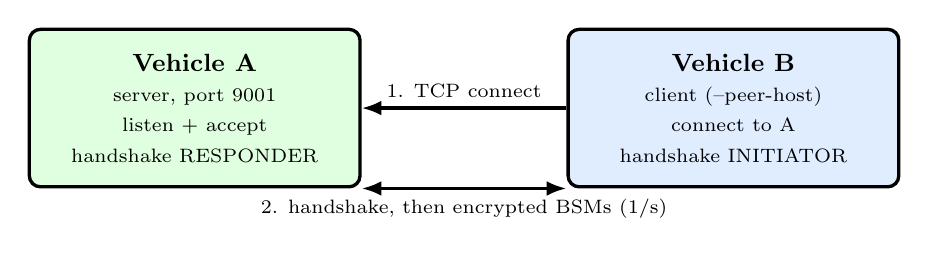
\begin{tikzpicture}[font=\small,node distance=8mm,
   v/.style={draw,very thick,rounded corners,minimum width=4.2cm,minimum height=2.0cm,
             align=center}]
  \node[v,fill=green!12] (a)
       {\textbf{Vehicle A}\\\scriptsize server, port 9001\\
        \scriptsize listen + accept\\\scriptsize handshake RESPONDER};
  \node[v,fill=boxblue,right=26mm of a] (b)
       {\textbf{Vehicle B}\\\scriptsize client (--peer-host)\\
        \scriptsize connect to A\\\scriptsize handshake INITIATOR};
  \draw[-{Latex[length=2.5mm]},very thick] (b) -- (a)
       node[midway,above,font=\scriptsize]{1. TCP connect};
  \draw[{Latex[length=2.5mm]}-{Latex[length=2.5mm]},very thick] (a.south east) -- (b.south west)
       node[midway,below,font=\scriptsize]{2. handshake, then encrypted BSMs (1/s)};
\end{tikzpicture}
\end{center}

\subsection{Diagram 2 --- length-prefix framing}
\begin{center}
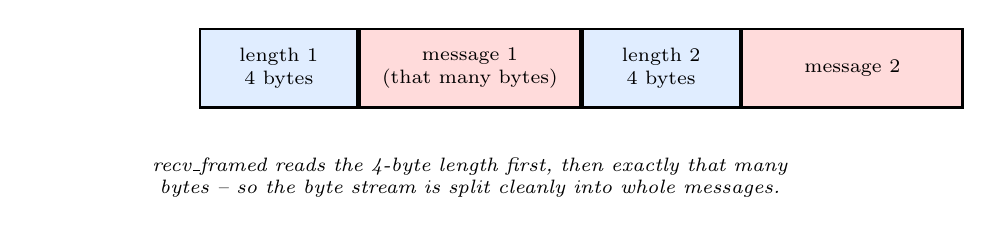
\begin{tikzpicture}[font=\scriptsize,node distance=4mm,
   f/.style={draw,thick,minimum height=1.0cm,align=center}]
  \node[f,fill=boxblue,minimum width=2.0cm] (h1) {length 1\\4 bytes};
  \node[f,fill=red!14,minimum width=2.8cm,right=0 of h1] (m1) {message 1\\(that many bytes)};
  \node[f,fill=boxblue,minimum width=2.0cm,right=0 of m1] (h2) {length 2\\4 bytes};
  \node[f,fill=red!14,minimum width=2.8cm,right=0 of h2] (m2) {message 2};
  \node[below=5mm of m1,font=\scriptsize\itshape,text width=11cm,align=center]
       {recv\_framed reads the 4-byte length first, then exactly that many bytes
        -- so the byte stream is split cleanly into whole messages.};
\end{tikzpicture}
\end{center}

\subsection{Diagram 3 --- the two communication threads}
\begin{center}
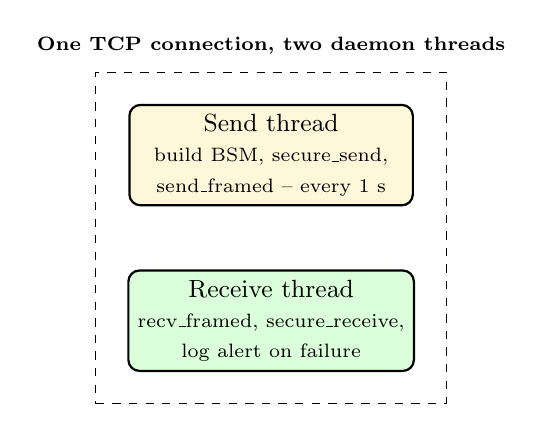
\begin{tikzpicture}[font=\small,node distance=7mm,
   t/.style={draw,thick,rounded corners,minimum width=3.6cm,minimum height=1.2cm,
             align=center}]
  \node[t,fill=boxyellow] (snd) {Send thread\\\scriptsize build BSM, secure\_send,\\\scriptsize send\_framed -- every 1 s};
  \node[t,fill=green!14,below=8mm of snd] (rcv) {Receive thread\\\scriptsize recv\_framed, secure\_receive,\\\scriptsize log alert on failure};
  \node[draw,dashed,fit=(snd)(rcv),inner sep=4mm] (box) {};
  \node[above=1mm of box,font=\scriptsize\bfseries] {One TCP connection, two daemon threads};
\end{tikzpicture}
\end{center}

% =====================================================================
\section{Presentation Pack}
% =====================================================================

\subsection{Slide Outline}

\textbf{Slide 1 --- From Library to Program.}
\begin{itemize}
  \item S2--S5 were libraries; S6 is the program you run.
  \item One file, \texttt{vehicle\_node.py}, launched once per car.
  \item It loads identity, runs the handshake, exchanges BSMs.
  \item It also starts the monitoring dashboard.
\end{itemize}

\textbf{Slide 2 --- TCP, Sockets and Framing.}
\begin{itemize}
  \item TCP = a reliable, ordered byte stream between two programs.
  \item But a stream has no message boundaries.
  \item Fix: a 4-byte length header before every message.
  \item \texttt{recv\_framed} reads the length, then exactly that many bytes.
\end{itemize}

\textbf{Slide 3 --- Server, Client and the Handshake.}
\begin{itemize}
  \item One car listens (server); the other connects (client).
  \item Client connects with up to 5 retries and exponential backoff.
  \item Client = handshake initiator; server = responder.
  \item A failed handshake (\texttt{AuthError}) $\to$ connection closed.
\end{itemize}

\textbf{Slide 4 --- Two Threads: Send and Receive.}
\begin{itemize}
  \item Sending and receiving must happen at the same time.
  \item Send thread: one encrypted BSM every second.
  \item Receive thread: decrypt + verify every incoming BSM.
  \item Both are daemon threads --- they stop when the program stops.
\end{itemize}

\textbf{Slide 5 --- Reacting to Attacks at Runtime.}
\begin{itemize}
  \item The receive loop wraps \texttt{secure\_receive} in try/except.
  \item \texttt{TamperError} $\to$ TAMPER ALERT, logged, keep running.
  \item \texttt{SequenceError} $\to$ REPLAY ALERT, logged, keep running.
  \item An attacker cannot crash the node with bad messages.
\end{itemize}

\subsection{Speaker Talking Points (about 30--60 seconds each)}

\textbf{Slide 1.} ``Everything we have built so far has been a library --- code
that other code calls. Section six is different: it is the actual program. You
launch vehicle\_node.py once for each car. It loads that car's certificate and
keys, opens a network connection to the other car, runs the four-step handshake,
and then settles into exchanging encrypted safety messages once a second. It even
starts the web dashboard. So this file is the conductor that brings sections two
through five together into one running system.''

\textbf{Slide 2.} ``The cars talk over TCP. TCP is like a reliable phone line ---
bytes arrive complete and in order. But TCP has one quirk: it delivers an
unbroken stream of bytes with no markers showing where one message stops and the
next starts. Imagine someone reading phone numbers aloud with no pauses. Our fix
is framing: before every message we write a four-byte number saying how long the
message is. The receiver reads those four bytes first, learns the length, then
reads exactly that many bytes --- one clean message, every time.''

\textbf{Slide 3.} ``Someone has to be reachable first, so one car is the server:
it opens a port and waits. The other is the client: it dials in. Because the two
laptops may start at different times, the client retries up to five times, and
waits a little longer before each retry --- two seconds, four, six --- so-called
exponential backoff. Once connected, the client plays the initiator in the
handshake and the server plays the responder. If the handshake fails --- a bad
certificate or a bad signature --- the code raises an AuthError and simply closes
the connection. No session, no messaging.''

\textbf{Slide 4.} ``A real conversation needs you to speak and listen at the same
time. A single line of code can only do one thing at once, so the node uses two
threads. The send thread builds a safety message, secures it, and sends it ---
once every second, forever. The receive thread waits for incoming messages,
decrypts and verifies each one. They run side by side. Both are daemon threads,
which just means they shut down automatically when the main program exits.''

\textbf{Slide 5.} ``Here is the security behaviour that matters at runtime. The
receive loop calls secure\_receive inside a try/except block. If a message has
been tampered with, secure\_receive throws a TamperError --- the loop catches it,
writes a TAMPER ALERT to the log, and carries on. A replayed message throws a
SequenceError and becomes a REPLAY ALERT. The node never crashes. So an attacker
flooding it with bad messages just fills the alert log --- they cannot take the
vehicle down.''

\subsection{Live-Demo Script}
\begin{enumerate}
  \item \textbf{Open two terminals.} Start Vehicle~A (server), then Vehicle~B
        (client) with the commands above.
  \item \textbf{Point at the handshake line.} \texttt{=== AUTHENTICATED with
        vehicle-a ===} --- ``the four-step handshake just ran over the network.''
  \item \textbf{Point at the BSM lines.} \texttt{BSM \#n sent} and \texttt{BSM
        \#n ... VERIFIED} --- ``send thread and receive thread, both running.''
  \item \textbf{Show robustness.} Mention that running an attack script against
        the node produces a TAMPER/REPLAY ALERT line but the node keeps going.
  \item \textbf{Optional.} Start B before A to show the retry/backoff messages.
\end{enumerate}

\subsection{Examiner Q\&A}
\begin{enumerate}
  \item \textbf{Q: What is TCP, and does it provide security here?}\\
        A: TCP is a reliable, ordered byte-stream protocol between two programs.
        It provides \emph{no} security --- the connection is plain. All security
        is in the SecureBSM payload (S5).
  \item \textbf{Q: What is the framing problem and how is it solved?}\\
        A: TCP gives a boundary-less byte stream. The fix is a 4-byte big-endian
        length header before each message; \texttt{recv\_framed} reads the length
        then exactly that many bytes.
  \item \textbf{Q: Why does \texttt{\_recv\_exactly} use a loop?}\\
        A: A single \texttt{recv} may return fewer bytes than requested, so the
        loop keeps reading until exactly \texttt{n} bytes are collected.
  \item \textbf{Q: What is the difference between the server and client?}\\
        A: The server binds a port and waits (\texttt{listen}/\texttt{accept});
        the client connects to the server's address. The client is the handshake
        initiator, the server the responder.
  \item \textbf{Q: Why are two threads needed?}\\
        A: Sending a BSM every second and receiving BSMs must happen
        simultaneously; one thread runs the send loop, the other the receive
        loop. Daemon threads stop automatically when the program exits.
  \item \textbf{Q: What is exponential backoff and why use it?}\\
        A: Waiting longer before each retry (2\,s, 4\,s, 6\,s...). It lets a
        slow-starting server come up without the client hammering the network.
  \item \textbf{Q: What happens when a tampered BSM arrives?}\\
        A: \texttt{secure\_receive} raises \texttt{TamperError}; the receive loop
        catches it, logs a TAMPER ALERT, and continues --- the node does not crash.
  \item \textbf{Q: Name a limitation of this networking design.}\\
        A: The server accepts exactly one peer (\texttt{listen(1)}), so it is a
        two-car simulation, not a scalable network. Also, traffic metadata
        (timing, sizes, the fact that two cars talk) is visible even though
        contents are protected.
\end{enumerate}

% =====================================================================
\section{Glossary}
% =====================================================================
\begin{description}[style=nextline,leftmargin=0pt]
  \item[TCP] Transmission Control Protocol: reliable, ordered byte-stream networking.
  \item[Socket] The software end point of a network connection.
  \item[Byte stream] A continuous flow of bytes with no message boundaries.
  \item[Framing] Adding markers so a stream can be split into messages.
  \item[Length-prefix] A length number written just before a message.
  \item[Big-endian] Byte order with the most significant byte first.
  \item[Server] The side that listens and waits to be contacted.
  \item[Client] The side that initiates the connection.
  \item[bind / listen / accept] Server socket steps: claim a port, mark ready, take a connection.
  \item[connect] The client socket step: dial the server.
  \item[Port] A numbered endpoint on a computer that a program listens behind.
  \item[0.0.0.0] ``All network interfaces'' --- bind on every local address.
  \item[SO\_REUSEADDR] A socket option allowing quick re-binding of a port after restart.
  \item[Thread] A separate line of execution inside one program.
  \item[Daemon thread] A thread that does not keep the program alive on its own.
  \item[Concurrency] Doing more than one task in overlapping time.
  \item[Exponential backoff] Waiting progressively longer before each retry.
  \item[Initiator / Responder] The two handshake roles (client / server here).
  \item[VehicleNode] The class representing one running vehicle.
  \item[secure\_send / secure\_receive] The S5 functions the loops call.
  \item[TamperError / SequenceError] Exceptions the receive loop catches and logs.
  \item[Metadata] Information about traffic (timing, size) rather than its content.
\end{description}

% =====================================================================
\section{References and Further Study}
% =====================================================================
\begin{itemize}
  \item \textbf{Python socket module documentation} ---
        \url{https://docs.python.org/3/library/socket.html}\\
        Read for: \texttt{bind}, \texttt{listen}, \texttt{accept},
        \texttt{connect}, \texttt{recv}, \texttt{sendall}.
  \item \textbf{Python socket programming HOWTO} ---
        \url{https://docs.python.org/3/howto/sockets.html}\\
        Read for: a beginner walk-through of client/server sockets and framing.
  \item \textbf{Python threading module documentation} ---
        \url{https://docs.python.org/3/library/threading.html}\\
        Read for: \texttt{Thread}, daemon threads, concurrency.
  \item \textbf{Transmission Control Protocol (Wikipedia)} ---
        \url{https://en.wikipedia.org/wiki/Transmission_Control_Protocol}\\
        Read for: what TCP guarantees and how it works.
  \item \textbf{Network socket (Wikipedia)} ---
        \url{https://en.wikipedia.org/wiki/Network_socket}\\
        Read for: the socket concept explained simply.
  \item \textbf{Exponential backoff (Wikipedia)} ---
        \url{https://en.wikipedia.org/wiki/Exponential_backoff}\\
        Read for: why retry delays grow.
  \item \textbf{Python struct module documentation} ---
        \url{https://docs.python.org/3/library/struct.html}\\
        Read for: the 4-byte big-endian length header (\texttt{">I"}).
  \item \textbf{Python argparse documentation} ---
        \url{https://docs.python.org/3/library/argparse.html}\\
        Read for: how the command-line options are parsed in \texttt{main}.
  \item \textbf{Beej's Guide to Network Programming} ---
        \url{https://beej.us/guide/bgnet/}\\
        Read for: a famous, friendly introduction to sockets and framing.
\end{itemize}

\vfill
\begin{center}\footnotesize\itshape
End of Section S6. Next: S7 --- the Flask monitoring dashboard that visualises
this running node.
\end{center}



% ===================== 07-monitoring-dashboard.tex =====================
\chapter{S7 --- The Monitoring Dashboard}

\section{Title and ``What You'll Learn''}
% =====================================================================

\subsection*{Section Title}
\textbf{S7 --- The Monitoring Dashboard: a small web page that lets a human
\emph{watch} the secure V2V system work in real time.}

\subsection*{Plain-English Summary (read this first)}
The security work is done by Sections~S2--S6. Section~S7 adds \emph{eyes}: a web
page, served by a tiny \textbf{Flask} web application, that shows --- live --- a
vehicle's certificate status, whether it has authenticated, how many messages it
has sent and received, and any security alerts. The browser asks the server
``what is happening now?'' every three seconds and re-draws the page. It is
crucial to understand that the dashboard is a \emph{window}, not a \emph{lock}:
it \emph{observes} security, it does not \emph{enforce} it.

\subsection*{Learning Outcomes}
After studying this section you will be able to:
\begin{itemize}
  \item Explain what \textbf{Flask}, a \textbf{web server} and an
        \textbf{HTTP route} are.
  \item Explain a \textbf{REST API} and the difference between \textbf{GET} and
        \textbf{POST}.
  \item Explain \textbf{JSON} as the language between browser and server.
  \item Explain \textbf{polling} and why the page refreshes every 3 seconds.
  \item Explain what \textbf{CORS} is and why it appears here.
  \item Walk through all four routes in \texttt{app.py} and the JavaScript in
        \texttt{dashboard.html}.
  \item Explain why the dashboard is \emph{observability}, not a security control.
\end{itemize}

% =====================================================================
\section{Where This Fits}
% =====================================================================

S7 sits \emph{beside} the pipeline, not inside it. The three security stages
(Identity, Authentication, Secure Messaging) run inside the vehicle node of S6.
S7 attaches a viewing window to that running node: \texttt{app.py} reads the
node's state through the \texttt{get\_state()} method (introduced in S6) and
serves it to a browser. If you removed S7 entirely, the cars would still
communicate just as securely --- you simply would not be able to \emph{see} it.

\begin{center}
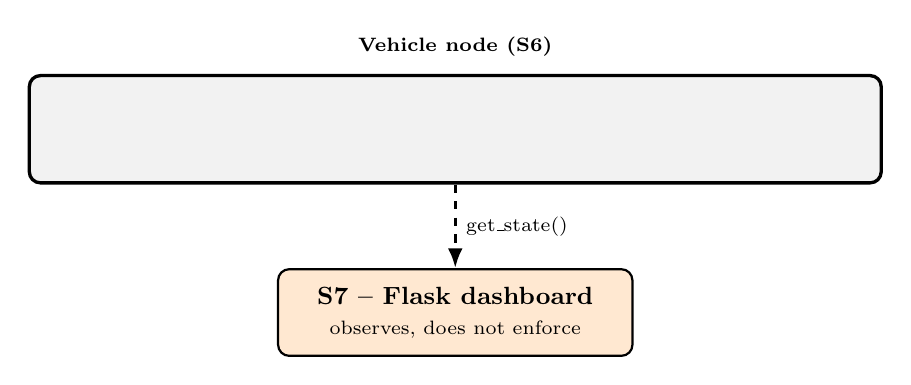
\begin{tikzpicture}[font=\small,node distance=8mm and 12mm,
   st/.style={draw,rounded corners,minimum width=2.7cm,minimum height=1.1cm,
              align=center,thick}]
  \node[st,fill=boxblue]   (id)   {Identity\\\scriptsize S2};
  \node[st,fill=green!12,right=of id]   (au) {Authentication\\\scriptsize S4};
  \node[st,fill=boxyellow,right=of au] (ms) {Messaging\\\scriptsize S5};
  \node[draw,very thick,rounded corners,fill=gray!10,fit=(id)(au)(ms)] (vn) {};
  \node[above=1mm of vn,font=\scriptsize\bfseries] {Vehicle node (S6)};
  \node[st,fill=orange!18,below=12mm of au,minimum width=4.5cm] (dash)
       {\textbf{S7 -- Flask dashboard}\\\scriptsize observes, does not enforce};
  \draw[-{Latex[length=2.5mm]},very thick,dashed] (vn) -- (dash)
       node[midway,right,font=\scriptsize]{get\_state()};
\end{tikzpicture}
\end{center}

% =====================================================================
\section{The Theory You Must Study}
% =====================================================================

\subsection{Web Server, Flask and HTTP}
\textbf{Plain definition.} A \textbf{web server} is a program that answers
requests from web browsers. \textbf{HTTP} (HyperText Transfer Protocol) is the
language of those requests and answers. \textbf{Flask} is a small, popular Python
library for building web servers.

\textbf{Real-life analogy.} A web server is an information desk. HTTP is the
fixed call-and-response format: a visitor asks a question (``request''), the desk
gives an answer (``response''). Flask is a starter kit for setting up that desk.

\textbf{Why it exists.} People want to \emph{see} the V2V system in an ordinary
web browser. A web server is what lets a browser ask for and receive a page.

\textbf{How it works here.} \texttt{app.py} calls \texttt{Flask(\_\_name\_\_)} to
create the server, then defines a few \emph{routes}. \texttt{vehicle\_node.py}
runs this Flask app in a background daemon thread.

\textbf{Security property it provides.} None --- the dashboard is a viewer.

\subsection{Routes / Endpoints}
\textbf{Plain definition.} A \textbf{route} (or \emph{endpoint}) is a specific
web address the server knows how to answer, paired with the code that produces
the answer.

\textbf{Real-life analogy.} The different windows at a post office: ``Stamps'',
``Parcels'', ``Complaints''. Each address goes to a specific window with specific
staff.

\textbf{Why it exists.} One server must answer several different questions ---
``give me the page'', ``give me the live data'', ``clear the alerts''. Routes
keep each question separate.

\textbf{How it works here.} The \texttt{@app.route("/...")} decorator above a
function says ``when a browser asks for this address, run this function''.
\texttt{app.py} defines four routes.

\textbf{Security property it provides.} None directly.

\subsection{REST API, GET and POST}
\textbf{Plain definition.} An \textbf{API} (Application Programming Interface) is
a way for one program to ask another for data or actions. A \textbf{REST API}
over HTTP uses different \emph{methods}: \textbf{GET} \emph{reads} data (and
changes nothing); \textbf{POST} \emph{sends} data or \emph{triggers a change}.

\textbf{Real-life analogy.} GET is \emph{looking at} the noticeboard. POST is
\emph{pinning a new note} to it. Looking changes nothing; pinning does.

\textbf{Why it exists.} The browser needs two kinds of interaction: fetch the
latest state (read) and clear the alerts (change). Using GET for reads and POST
for changes keeps the design clean and predictable.

\textbf{How it works here.} \texttt{/api/state} and \texttt{/api/alerts} are GET
routes (read-only). \texttt{/api/clear-alerts} is a POST route
(\texttt{methods=["POST"]}) because it changes something --- it empties the alert
list.

\textbf{Security property it provides.} None directly, though using GET only for
safe reads is good hygiene.

\subsection{JSON --- the Browser/Server Language}
\textbf{Plain definition.} \textbf{JSON} (JavaScript Object Notation) is a simple
text format for structured data --- names paired with values, in braces.

\textbf{Real-life analogy.} A filled-in form with labelled boxes:
\texttt{vehicle\_id: vehicle-a, total\_sent: 42}.

\textbf{Why it exists.} The Python server and the JavaScript in the browser are
different languages, but both understand JSON, so it is the neutral format they
exchange.

\textbf{How it works here.} Flask's \texttt{jsonify(...)} turns a Python
dictionary into a JSON response. In the browser, \texttt{await r.json()} turns
that JSON text back into a JavaScript object the page can read.

\textbf{Security property it provides.} None --- it is a data format.

\subsection{Polling}
\textbf{Plain definition.} \textbf{Polling} means the browser repeatedly asks
``anything new?'' on a timer, rather than the server pushing updates.

\textbf{Real-life analogy.} Refreshing your email inbox every few minutes instead
of waiting for a notification.

\textbf{Why it exists.} It is the \emph{simplest} way to keep a page up to date.
The dashboard does not need split-second freshness, so a humble timer is enough
--- no need for more complex ``push'' technology.

\textbf{How it works here.} The JavaScript line \texttt{setInterval(fetchState,
3000)} runs \texttt{fetchState} every 3000~milliseconds (3 seconds). Each call
fetches \texttt{/api/state} and redraws the page.

\textbf{Security property it provides.} None.

\subsection{CORS}
\textbf{Plain definition.} \textbf{CORS} (Cross-Origin Resource Sharing) is a
browser security rule that, by default, stops a page loaded from one web address
from reading data from a \emph{different} address. A server can relax this rule
with special response headers.

\textbf{Real-life analogy.} A building security rule: a visitor with a ``Floor~5''
pass cannot wander onto Floor~3. CORS headers are the management explicitly
saying ``actually, let this pass work on Floor~3 too''.

\textbf{Why it exists here.} Vehicle~A's dashboard runs on port~5001 and
Vehicle~B's on port~5002 --- the browser treats those as different ``origins''.
To let a page on one port read the API on another, the server must allow it.

\textbf{How it works here.} An \texttt{@app.after\_request} hook adds the header
\texttt{Access-Control-Allow-Origin: *}. The \texttt{*} means ``any origin may
read this API''.

\textbf{Security property it provides.} CORS is itself a security mechanism ---
but here it is \emph{loosened} to \texttt{*}. That is fine for a local classroom
demo, but in a real deployment an open \texttt{*} on an unauthenticated API would
be a weakness. (More on this in the Attack Relevance section.)

% =====================================================================
\section{Code Walkthrough}
% =====================================================================

\subsection{File: dashboard/app.py --- the Flask server}

\subsubsection*{create\_app() --- build the web application}
\textbf{Purpose:} create the Flask app, bind it to a running vehicle node, and
define the routes.
\begin{lstlisting}[style=py,caption={dashboard/app.py --- the whole Flask application.}]
def create_app(node) -> Flask:
    app = Flask(__name__,
                template_folder=str(Path(__file__).parent / "templates"))

    @app.after_request
    def _cors(response):
        response.headers["Access-Control-Allow-Origin"] = "*"
        response.headers["Access-Control-Allow-Methods"] = "GET, POST, OPTIONS"
        response.headers["Access-Control-Allow-Headers"] = "Content-Type"
        return response

    @app.route("/")
    def index():
        return render_template("dashboard.html")

    @app.route("/api/state")
    def api_state():
        return jsonify(node.get_state())

    @app.route("/api/alerts")
    def api_alerts():
        return jsonify({"alerts": node.logger.get_alerts()})

    @app.route("/api/clear-alerts", methods=["POST"])
    def api_clear_alerts():
        node.logger.clear_alerts()
        return jsonify({"status": "cleared"})

    return app
\end{lstlisting}
\textbf{Step by step:}
\begin{enumerate}
  \item \texttt{create\_app(node)} takes the running \texttt{VehicleNode} (from
        S6) so the dashboard has a live data source.
  \item \texttt{Flask(...)} creates the server; \texttt{template\_folder} tells
        it where the HTML page lives.
  \item The \texttt{\_cors} function, marked \texttt{@app.after\_request}, runs
        \emph{after every response} and adds the CORS headers (see the theory
        above).
  \item Route \texttt{"/"} --- the home page. \texttt{render\_template} loads and
        returns \texttt{dashboard.html}.
  \item Route \texttt{"/api/state"} --- a GET endpoint. It calls the node's
        \texttt{get\_state()} and \texttt{jsonify}s the dictionary. This is the
        endpoint the browser polls every 3 seconds.
  \item Route \texttt{"/api/alerts"} --- a GET endpoint returning just the alert
        list.
  \item Route \texttt{"/api/clear-alerts"} --- a POST endpoint
        (\texttt{methods=["POST"]}) because it \emph{changes} state: it calls
        \texttt{clear\_alerts()} and confirms with \texttt{\{"status":
        "cleared"\}}.
\end{enumerate}
\textbf{Arguments / return:} \texttt{create\_app} takes \texttt{node} and returns
the Flask \texttt{app}; \texttt{vehicle\_node.py} then runs it in a thread.
\textbf{Theory link:} routes, REST (GET vs POST), JSON, CORS.
\emph{Analogy:} \texttt{app.py} is the information desk; each route is one
window.

\subsubsection*{The data source: node.get\_state()}
\texttt{app.py} itself produces no data --- it is a thin layer. The real content
comes from the vehicle node's \texttt{get\_state()} method (studied in S6), which
returns a dictionary of: \texttt{vehicle\_id}, certificate status and expiry,
authentication status, peer id, whether a session is active, the recent messages,
the alert list, and the statistics counters. \texttt{/api/state} just wraps that
dictionary in JSON.

\subsection{File: dashboard.html --- the page and its JavaScript}

\subsubsection*{The page structure (HTML)}
The HTML body has four visible regions:
\begin{enumerate}
  \item A \textbf{header} with the title.
  \item Three \textbf{status cards}: ``Certificate Status'', ``Authentication
        Status'' and ``Security Alerts'' (the last one has a \emph{Clear Alerts}
        button).
  \item A \textbf{stats row} of four boxes: Messages Sent, Messages Received,
        Attacks Blocked, Session Active.
  \item A \textbf{Recent Messages table} with one row per message and a tick/cross
        for each security property.
\end{enumerate}
Every value on the page starts as a placeholder (\texttt{--} or \texttt{LOADING})
and is filled in by JavaScript once the first data arrives.

\subsubsection*{The CSS (styling) --- one security-relevant detail}
Most of the CSS is cosmetic (a dark theme, rounded cards). One rule \emph{is}
worth noting --- the blinking-alert animation:
\begin{lstlisting}[style=web,caption={dashboard.html --- the alert-blink CSS (decorative comment dashes simplified).}]
/* -- Blinking alert card -- */
@keyframes blink-red {
  0%, 100% { border-color: #f85149; box-shadow: 0 0 15px rgba(248,81,73,0.4); }
  50%      { border-color: #30363d; box-shadow: none; }
}
.alert-active { animation: blink-red 1s infinite; }
\end{lstlisting}
When JavaScript adds the class \texttt{alert-active} to the alert card, this
animation makes it flash red once per second --- so a security alert is
impossible to miss on screen.

\subsubsection*{The JavaScript --- fetch, update, repeat}
\begin{lstlisting}[style=web,caption={dashboard.html --- the polling JavaScript (core parts).}]
async function fetchState() {
  try {
    const r = await fetch('/api/state');   // GET the live state
    const d = await r.json();              // parse JSON into an object
    update(d);                             // redraw the page
  } catch (e) { console.error('Fetch failed', e); }
}

function update(d) {
  // Certificate card
  const cb = document.getElementById('cert-badge');
  cb.textContent = d.cert_status;
  cb.className = 'badge ' + (d.cert_status === 'VALID' ? 'badge-green' : 'badge-red');
  // Alert card -- turn the card red and blinking if there are alerts
  const alerts = d.alerts || [];
  if (alerts.length > 0) {
    document.getElementById('alert-card').classList.add('alert-active');
  } else {
    document.getElementById('alert-card').classList.remove('alert-active');
  }
  // Stats: Attacks Blocked = tamper blocked + replay blocked
  const s = d.stats || {};
  document.getElementById('stat-blocked').textContent =
      (s.tamper_attempts_blocked || 0) + (s.replay_attempts_blocked || 0);
  // ... fill the message table row by row ...
}

async function clearAlerts() {
  await fetch('/api/clear-alerts', { method: 'POST' });   // POST
  fetchState();
}

setInterval(fetchState, 3000);   // poll every 3 seconds
fetchState();                    // and once immediately
\end{lstlisting}
\textbf{Step by step:}
\begin{enumerate}
  \item \texttt{fetchState} is \texttt{async} --- it sends a GET request to
        \texttt{/api/state}, \texttt{await}s the reply, and parses the JSON.
  \item \texttt{update(d)} takes that data object and writes it into the page:
        it sets the certificate badge text and colour, shows/clears the blinking
        alert state, fills the four stat boxes (note ``Attacks Blocked'' is the
        \emph{sum} of tamper and replay counters), and rebuilds the message
        table.
  \item \texttt{clearAlerts} sends a \texttt{POST} to \texttt{/api/clear-alerts}
        (this is the only state-changing call the page makes), then immediately
        refetches.
  \item \texttt{setInterval(fetchState, 3000)} repeats the fetch every 3 seconds;
        the bare \texttt{fetchState()} call runs once at page load so the user
        does not wait 3 seconds for the first data.
\end{enumerate}
\textbf{Theory link:} polling; GET for reads, POST for the change; JSON as the
shared format. \emph{Analogy:} a receptionist who phones the back office every 3
seconds and re-writes the whiteboard with the latest news.

% =====================================================================
\section{Hands-On / Practical}
% =====================================================================

\subsection{Open the dashboard}
Start a vehicle node as in Section~S6 (it launches the dashboard automatically),
then open a browser at the dashboard address printed in the log:
\begin{lstlisting}[style=term]
http://localhost:5001        (Vehicle A)
http://localhost:5002        (Vehicle B)
\end{lstlisting}

\noindent You can also confirm the API directly without a browser, using
PowerShell:
\begin{lstlisting}[style=term]
curl http://localhost:5001/api/state
\end{lstlisting}

\noindent\textbf{Expected output (sample of the \texttt{/api/state} JSON):}
\begin{lstlisting}[style=term]
{
  "vehicle_id": "vehicle-a",
  "cert_status": "VALID",
  "cert_cn": "vehicle-a",
  "cert_expiry": "2027-05-17",
  "auth_status": "AUTHENTICATED",
  "peer_id": "vehicle-b",
  "session_active": true,
  "recent_messages": [ ... ],
  "alerts": [],
  "stats": {"total_sent": 12, "total_received": 11,
            "tamper_attempts_blocked": 0, "replay_attempts_blocked": 0}
}
\end{lstlisting}

\subsection{What the dashboard shows}
\begin{itemize}
  \item \textbf{Certificate Status card} --- \texttt{VALID} (green) if the
        vehicle's certificate parsed correctly.
  \item \textbf{Authentication Status card} --- \texttt{AUTHENTICATED} (green)
        once the handshake has completed; shows the peer id.
  \item \textbf{Security Alerts card} --- \texttt{0 ALERTS} (green) normally; if
        an attack is blocked it turns red and \emph{blinks}.
  \item \textbf{Stats row} --- live counts of messages sent, received, attacks
        blocked, and whether a session is active.
  \item \textbf{Recent Messages table} --- the last 20 messages, each with
        green ticks for Auth / Encrypted / Integrity / Replay-protected.
\end{itemize}

\subsection{Illustration placeholder --- dashboard screenshot}
\begin{center}
\fbox{\parbox{0.85\textwidth}{\centering\vspace{1.2cm}
\textbf{[ ADD SCREENSHOT HERE ]}\\[4pt]
Run a vehicle node, open \texttt{http://localhost:5001} in a browser, take a
screenshot of the live dashboard, save it as \texttt{dashboard.png} in this
folder, and replace this box with:\\[4pt]
\texttt{\textbackslash includegraphics[width=0.85\textbackslash textwidth]\{dashboard.png\}}
\vspace{1.2cm}}}
\end{center}

\subsection{Try This Yourself (mini-experiment)}
With the two vehicle nodes running and the dashboard open, run an attack script
against the system (for example \texttt{python attacks\textbackslash
tamper\_attack.py}, Section~S8) --- or simply note what \emph{would} happen:
when a TAMPER or REPLAY alert is logged, the node's \texttt{get\_state()} returns
a non-empty \texttt{alerts} list.\\
\textbf{Predict before you run.} On the \emph{next} 3-second poll, the JavaScript
\texttt{update} function sees \texttt{alerts.length > 0}, adds the
\texttt{alert-active} class to the alert card, and the card starts blinking red;
the ``Attacks Blocked'' number ticks up. Now click \emph{Clear Alerts}: a POST is
sent, the alert list empties, and on the next poll the card goes calm green
again. As a second experiment, change \texttt{setInterval(fetchState, 3000)} to
\texttt{1000} --- predict the page now refreshes once per second instead of every
three.

% =====================================================================
\section{Attack Relevance}
% =====================================================================

\textbf{The dashboard defends against \emph{nothing}.} This is the single most
important point of S7, and an examiner will test it. The dashboard is
\textbf{observability}: it makes the work of the real defences \emph{visible to a
human}. It is the difference between a smoke alarm (a defence-adjacent alert) and
the sprinkler system (the actual defence).

\medskip
\noindent What the dashboard \emph{does} contribute:
\begin{itemize}
  \item It \textbf{surfaces} blocked attacks. When S5/S6 reject a tampered or
        replayed message, the alert is logged; the dashboard turns it into a
        blinking red card and an ``Attacks Blocked'' counter --- so a human
        immediately sees the system is under attack and is holding.
  \item It builds \textbf{confidence}: the green ticks per message let an
        observer confirm every BSM really was authenticated, encrypted,
        integrity-checked and replay-protected.
\end{itemize}

\medskip
\noindent\textbf{Honest weaknesses of the dashboard itself.} If an examiner asks
``could the dashboard be attacked?'', the honest answer is yes, in two ways, and
neither affects the V2V security itself:
\begin{enumerate}
  \item \textbf{The API is unauthenticated.} Anyone who can reach port~5001 can
        \texttt{GET /api/state} and read the vehicle's status, or
        \texttt{POST /api/clear-alerts} to wipe the alert history. There is no
        password on the dashboard.
  \item \textbf{CORS is wide open} (\texttt{Access-Control-Allow-Origin: *}), so
        any web page in the browser could read the API.
\end{enumerate}
For a local classroom demo this is acceptable and is a deliberate simplification.
In a real deployment the monitoring interface would need authentication and a
restricted CORS policy. Crucially, even if an attacker cleared the alert log,
they would \emph{not} weaken the cars' encryption, signatures or handshake ---
they would only blind the \emph{viewer}.

% =====================================================================
\section{Illustrations}
% =====================================================================

\subsection{Diagram 1 --- browser, Flask and the vehicle node}
\begin{center}
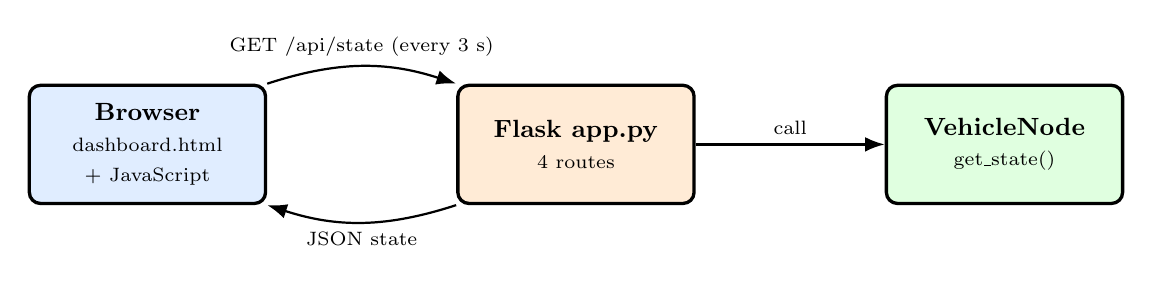
\begin{tikzpicture}[font=\small,node distance=14mm,
   b/.style={draw,very thick,rounded corners,minimum width=3.0cm,minimum height=1.5cm,
             align=center}]
  \node[b,fill=boxblue]  (br) {\textbf{Browser}\\\scriptsize dashboard.html\\\scriptsize + JavaScript};
  \node[b,fill=orange!16,right=24mm of br] (fl) {\textbf{Flask app.py}\\\scriptsize 4 routes};
  \node[b,fill=green!12,right=24mm of fl] (nd) {\textbf{VehicleNode}\\\scriptsize get\_state()};
  \draw[-{Latex[length=2.5mm]},thick] (br.north east) to[bend left=18]
       node[midway,above,font=\scriptsize]{GET /api/state (every 3 s)} (fl.north west);
  \draw[{Latex[length=2.5mm]}-,thick] (br.south east) to[bend right=18]
       node[midway,below,font=\scriptsize]{JSON state} (fl.south west);
  \draw[-{Latex[length=2.5mm]},thick] (fl) -- (nd)
       node[midway,above,font=\scriptsize]{call};
\end{tikzpicture}
\end{center}

\subsection{Diagram 2 --- the polling loop}
\begin{center}
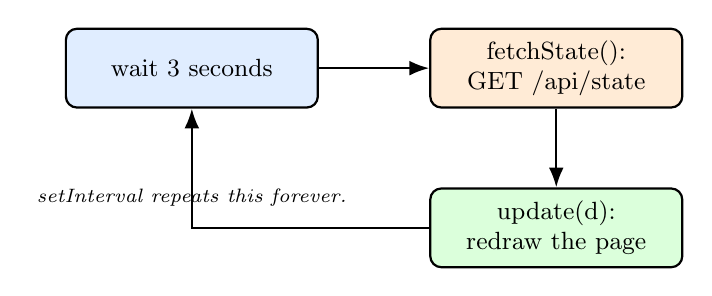
\begin{tikzpicture}[font=\small,node distance=9mm,
   s/.style={draw,thick,rounded corners,minimum width=3.2cm,minimum height=1.0cm,
             align=center}]
  \node[s,fill=boxblue] (wait) {wait 3 seconds};
  \node[s,fill=orange!16,right=14mm of wait] (fetch) {fetchState():\\GET /api/state};
  \node[s,fill=green!14,below=10mm of fetch] (upd) {update(d):\\redraw the page};
  \draw[-{Latex[length=2.5mm]},thick] (wait) -- (fetch);
  \draw[-{Latex[length=2.5mm]},thick] (fetch) -- (upd);
  \draw[-{Latex[length=2.5mm]},thick] (upd) -| (wait);
  \node[below=9mm of wait,font=\scriptsize\itshape] {setInterval repeats this forever.};
\end{tikzpicture}
\end{center}

% =====================================================================
\section{Presentation Pack}
% =====================================================================

\subsection{Slide Outline}

\textbf{Slide 1 --- What the Dashboard Is.}
\begin{itemize}
  \item A small web page that shows the V2V system live.
  \item Built with Flask (a Python web framework).
  \item Shows certificates, authentication, stats, alerts.
  \item It is a \emph{window}, not a \emph{lock}.
\end{itemize}

\textbf{Slide 2 --- How the Browser and Server Talk.}
\begin{itemize}
  \item Four routes: the page, state, alerts, clear-alerts.
  \item GET reads data; POST changes data.
  \item They exchange JSON --- the shared data format.
  \item CORS headers allow the cross-port setup.
\end{itemize}

\textbf{Slide 3 --- Polling: Always Up to Date.}
\begin{itemize}
  \item \texttt{setInterval(fetchState, 3000)} --- ask every 3 seconds.
  \item \texttt{fetchState} GETs \texttt{/api/state}, parses JSON.
  \item \texttt{update} redraws cards, stats and the message table.
  \item Simple timer; no complex push technology needed.
\end{itemize}

\textbf{Slide 4 --- Seeing an Attack.}
\begin{itemize}
  \item Blocked attacks become alerts in the node's logger.
  \item The alert card turns red and \emph{blinks}.
  \item ``Attacks Blocked'' = tamper blocked + replay blocked.
  \item \emph{Clear Alerts} button POSTs to reset the list.
\end{itemize}

\textbf{Slide 5 --- Observability, Not Enforcement.}
\begin{itemize}
  \item The dashboard defends nothing --- S2--S6 do that.
  \item It makes the defences visible and builds confidence.
  \item Honest weakness: the API has no password; CORS is open.
  \item Clearing alerts blinds the viewer --- it does not weaken the cars.
\end{itemize}

\subsection{Speaker Talking Points (about 30--60 seconds each)}

\textbf{Slide 1.} ``Sections two through six do the actual security work. Section
seven adds eyes. It is a small web page, served by a tiny Python web application
built with Flask, that shows the system working in real time --- the
certificate's status, whether the cars have authenticated, how many messages have
flowed, and any security alerts. The key idea, and I will keep repeating it, is
that this dashboard is a window, not a lock. It lets you watch the security; it
does not provide the security.''

\textbf{Slide 2.} ``The browser and the server talk over HTTP using four routes.
One route serves the HTML page itself. One returns the live state. One returns
just the alerts. And one clears the alerts. There is a deliberate split here: the
read-only routes use the GET method, and the one route that changes something ---
clearing the alerts --- uses POST. Looking at a noticeboard versus pinning a new
note. They exchange data as JSON, a text format both Python and JavaScript
understand, and a CORS header lets the two dashboards on different ports work
together.''

\textbf{Slide 3.} ``How does the page stay current? By polling. There is one line
of JavaScript --- setInterval, fetchState, three thousand milliseconds --- that
says: every three seconds, ask the server for the latest state. Each time,
fetchState sends a GET request, gets JSON back, and the update function rewrites
the page: the cards, the statistics, the message table. It is not the most
sophisticated technique, but the dashboard does not need split-second freshness,
so a simple timer is exactly right.''

\textbf{Slide 4.} ``When the security system blocks an attack --- a tampered or
replayed message --- it records an alert. The dashboard turns that alert into
something a human cannot miss: the alerts card flips to red and blinks once a
second, and the `Attacks Blocked' counter, which is the tamper count plus the
replay count, ticks up. There is also a Clear Alerts button; pressing it sends a
POST request that empties the alert list, and the card calms down on the next
poll.''

\textbf{Slide 5.} ``Let me be very clear about the dashboard's role, because it
is a favourite exam question. The dashboard enforces nothing. If you deleted it,
the cars would be exactly as secure. What it adds is observability --- it makes
the invisible defences visible, and the green ticks let you confirm every message
really was protected. And honestly, the dashboard has its own weak spots: the API
has no password, and CORS is wide open. For a classroom demo that is fine. But
note: even an attacker who cleared the alert log would only blind the viewer ---
the encryption, the signatures and the handshake would all still hold.''

\subsection{Live-Demo Script}
\begin{enumerate}
  \item \textbf{Start the system.} Launch two vehicle nodes (S6). Open
        \texttt{http://localhost:5001} and \texttt{http://localhost:5002}.
  \item \textbf{Point at the cards.} Certificate VALID, Authentication
        AUTHENTICATED --- ``green means the security stages succeeded.''
  \item \textbf{Point at the table.} The message rows with green ticks ---
        ``every BSM authenticated, encrypted, integrity-checked.''
  \item \textbf{Show the API.} In a terminal run \texttt{curl
        http://localhost:5001/api/state} --- ``this raw JSON is what the page
        polls every 3 seconds.''
  \item \textbf{Trigger and clear an alert.} Run an attack script (S8); watch the
        alert card blink red; press \emph{Clear Alerts} and watch it reset.
\end{enumerate}

\subsection{Examiner Q\&A}
\begin{enumerate}
  \item \textbf{Q: Does the dashboard make the system more secure?}\\
        A: No. It is observability, not enforcement. It \emph{shows} the security
        worked; it does not provide it. Removing it leaves the cars equally
        secure.
  \item \textbf{Q: What is Flask and what are routes?}\\
        A: Flask is a small Python web framework. A route maps a web address
        (e.g.\ \texttt{/api/state}) to the function that produces its response.
  \item \textbf{Q: Why is \texttt{/api/clear-alerts} a POST and the others GET?}\\
        A: GET is for safe reads that change nothing; POST is for actions that
        change state. Clearing the alert list changes state, so it is POST.
  \item \textbf{Q: How does the page stay up to date?}\\
        A: Polling --- \texttt{setInterval(fetchState, 3000)} fetches
        \texttt{/api/state} every 3 seconds and the \texttt{update} function
        redraws the page.
  \item \textbf{Q: What is JSON used for here?}\\
        A: It is the shared data format. Flask's \texttt{jsonify} sends Python
        data as JSON; the browser's \texttt{r.json()} parses it back.
  \item \textbf{Q: What is CORS and how is it configured?}\\
        A: A browser rule limiting cross-origin reads. The \texttt{after\_request}
        hook sets \texttt{Access-Control-Allow-Origin: *}, allowing any origin
        --- fine for a demo, too permissive for production.
  \item \textbf{Q: Where does the dashboard's data come from?}\\
        A: From the vehicle node's \texttt{get\_state()} method (S6);
        \texttt{app.py} only wraps that dictionary as JSON.
  \item \textbf{Q: Could clearing the alerts help an attacker?}\\
        A: Only cosmetically --- it blinds the human viewer. It does not touch
        the encryption, signatures or handshake, so the cars stay secure.
\end{enumerate}

% =====================================================================
\section{Glossary}
% =====================================================================
\begin{description}[style=nextline,leftmargin=0pt]
  \item[Dashboard] A web page that displays the live state of the system.
  \item[Web server] A program that answers requests from web browsers.
  \item[Flask] A small Python web framework used to build the server.
  \item[HTTP] HyperText Transfer Protocol: the request/response language of the web.
  \item[Route / endpoint] A web address paired with the code that answers it.
  \item[API] Application Programming Interface: a way for programs to ask for data/actions.
  \item[REST] A style of HTTP API using methods like GET and POST.
  \item[GET] An HTTP method for reading data (changes nothing).
  \item[POST] An HTTP method for sending data or triggering a change.
  \item[JSON] JavaScript Object Notation: a text format for structured data.
  \item[jsonify] The Flask function that turns Python data into a JSON response.
  \item[render\_template] The Flask function that returns an HTML page.
  \item[Polling] Repeatedly asking the server for updates on a timer.
  \item[setInterval] The JavaScript function that runs code on a repeating timer.
  \item[fetch] The browser function that sends an HTTP request.
  \item[CORS] Cross-Origin Resource Sharing: a browser rule on cross-address reads.
  \item[Origin] A web address identity (scheme + host + port).
  \item[after\_request] A Flask hook that runs after every response is built.
  \item[Observability] The ability to see what a system is doing.
  \item[Enforcement] Actually preventing/blocking bad behaviour (what S2--S6 do).
  \item[get\_state()] The VehicleNode method that supplies the dashboard's data.
  \item[Alert] A recorded security event (a blocked tamper or replay).
\end{description}

% =====================================================================
\section{References and Further Study}
% =====================================================================
\begin{itemize}
  \item \textbf{Flask documentation --- Quickstart} ---
        \url{https://flask.palletsprojects.com/en/latest/quickstart/}\\
        Read for: routes, \texttt{render\_template}, \texttt{jsonify}.
  \item \textbf{Flask documentation --- application factories} ---
        \url{https://flask.palletsprojects.com/en/latest/patterns/appfactories/}\\
        Read for: the \texttt{create\_app(node)} pattern used here.
  \item \textbf{MDN --- An overview of HTTP} ---
        \url{https://developer.mozilla.org/en-US/docs/Web/HTTP/Overview}\\
        Read for: how HTTP requests and responses work.
  \item \textbf{MDN --- HTTP request methods (GET, POST)} ---
        \url{https://developer.mozilla.org/en-US/docs/Web/HTTP/Methods}\\
        Read for: the difference between GET and POST.
  \item \textbf{MDN --- Cross-Origin Resource Sharing (CORS)} ---
        \url{https://developer.mozilla.org/en-US/docs/Web/HTTP/CORS}\\
        Read for: what CORS is and why the \texttt{*} header matters.
  \item \textbf{MDN --- Using the Fetch API} ---
        \url{https://developer.mozilla.org/en-US/docs/Web/API/Fetch_API/Using_Fetch}\\
        Read for: the \texttt{fetch} calls in \texttt{dashboard.html}.
  \item \textbf{MDN --- setInterval} ---
        \url{https://developer.mozilla.org/en-US/docs/Web/API/setInterval}\\
        Read for: how the 3-second polling timer works.
  \item \textbf{JSON (Wikipedia)} ---
        \url{https://en.wikipedia.org/wiki/JSON}\\
        Read for: the JSON data format.
  \item \textbf{REST (Wikipedia)} ---
        \url{https://en.wikipedia.org/wiki/REST}\\
        Read for: the REST API style.
  \item \textbf{OWASP API Security Top 10} ---
        \url{https://owasp.org/API-Security/editions/2023/en/0x11-t10/}\\
        Read for: why an unauthenticated, open-CORS API is a real-world weakness.
\end{itemize}

\vfill
\begin{center}\footnotesize\itshape
End of Section S7. Next: S8 --- the attack scripts that try to break the system
the dashboard is watching.
\end{center}



% ===================== 08-attack-demonstrations.tex =====================
\chapter{S8 --- Attack Demonstrations}

\section{Title and ``What You'll Learn''}
% =====================================================================

\subsection*{Section Title}
\textbf{S8 --- Attack Demonstrations: three short scripts that play the role of
the attacker and prove, on screen, that the defences actually work.}

\subsection*{Plain-English Summary (read this first)}
A security claim means nothing until you \emph{try to break it}. Section~S8 is
the project's ``red team'': three Python scripts that each \emph{become the
attacker}. \texttt{replay\_attack.py} captures a real message and re-sends it
late. \texttt{tamper\_attack.py} intercepts a message and flips bits in it.
\texttt{mitm\_attack.py} plays the man-in-the-middle in two ways --- a fake
certificate and a forged signature. Each script runs the attack against the real
project code and prints \texttt{[BLOCKED]} when the defence stops it. S8 does not
add any new defence --- it \emph{tests} the defences of S2--S5.

\subsection*{Learning Outcomes}
After studying this section you will be able to:
\begin{itemize}
  \item Explain \textbf{adversarial testing} (red-teaming) and why it matters.
  \item Describe exactly how a \textbf{replay}, a \textbf{tamper} and a
        \textbf{man-in-the-middle} attack are performed.
  \item Walk through each attack script step by step.
  \item Name the precise defence (and which section) that blocks each attack.
  \item Run all three scripts, read their output, and explain every line.
  \item Honestly explain the limits of each demonstration.
\end{itemize}

% =====================================================================
\section{Where This Fits}
% =====================================================================

S8 sits \emph{against} the whole pipeline. The earlier sections \emph{claim}
six security properties; S8 is where those claims are put on trial. Each script
imports the real project modules --- the same \texttt{crypto.py},
\texttt{auth\_protocol.py} and \texttt{v2v\_protocol.py} the vehicles use --- and
attacks them. If a defence were broken, the script would print \texttt{[FAIL]}.

\begin{center}
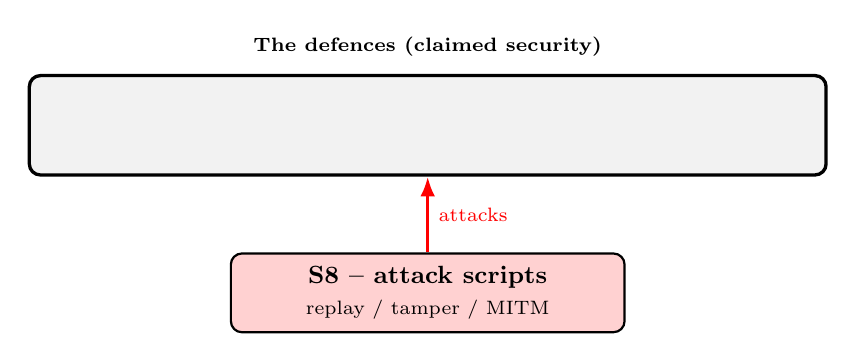
\begin{tikzpicture}[font=\small,node distance=7mm and 10mm,
   st/.style={draw,rounded corners,minimum width=2.6cm,minimum height=1.0cm,
              align=center,thick}]
  \node[st,fill=boxblue]   (id)   {Identity\\\scriptsize S2};
  \node[st,fill=green!12,right=of id]   (au) {Authentication\\\scriptsize S4};
  \node[st,fill=boxyellow,right=of au] (ms) {Messaging\\\scriptsize S5};
  \node[draw,very thick,rounded corners,fill=gray!10,fit=(id)(au)(ms)] (def) {};
  \node[above=1mm of def,font=\scriptsize\bfseries] {The defences (claimed security)};
  \node[st,fill=red!18,below=11mm of au,minimum width=5cm] (atk)
       {\textbf{S8 -- attack scripts}\\\scriptsize replay / tamper / MITM};
  \draw[-{Latex[length=2.5mm]},very thick,red] (atk) -- (def)
       node[midway,right,font=\scriptsize]{attacks};
\end{tikzpicture}
\end{center}

% =====================================================================
\section{The Theory You Must Study}
% =====================================================================

\subsection{Adversarial Testing (Red-Teaming)}
\textbf{Plain definition.} \emph{Adversarial testing} means deliberately
attacking your own system to check the defences hold. A \emph{red team} is the
group (or here, the scripts) that plays the attacker.

\textbf{Real-life analogy.} A locksmith does not just \emph{say} a lock is good
--- they hire someone to try every trick to pick it. If it opens, the lock is
not good.

\textbf{Why it exists.} Designers are optimistic; they trust their own code. An
attacker is not bound by the designer's assumptions. Testing from the attacker's
side finds the gap between ``should be secure'' and ``is secure''.

\textbf{How it works here.} Three scripts each import the genuine project modules
and perform a real attack against them, then report \texttt{[BLOCKED]} or
\texttt{[FAIL]}.

\textbf{Security property it relates to.} It validates \emph{all} of them ---
S8 is the evidence behind the project's security claims.

\subsection{The Replay Attack}
\textbf{Plain definition.} The attacker records a genuine, valid encrypted
message and sends the \emph{exact same bytes} again later.

\textbf{Real-life analogy.} Secretly recording someone saying ``open the garage''
and playing the recording back tomorrow.

\textbf{Why it is dangerous.} The replayed message is \emph{perfectly valid} ---
correct encryption, correct signature. Nothing is forged. The only thing wrong is
that it is \emph{old}. Re-sending an old ``I am braking!'' could trigger needless
braking and a crash.

\textbf{How the script does it.} \texttt{replay\_attack.py} sends a BSM, lets it
be received once (which succeeds), waits \textbf{6 seconds} --- one second past
the 5-second freshness window --- then re-sends the identical bytes.

\textbf{The defence that stops it.} The \texttt{TimestampValidator} (S4/S5): the
message's timestamp is now more than 5 seconds old, so
\texttt{secure\_receive} raises \texttt{StaleMessageError}. The sequence-number
check is a second line of defence.

\subsection{The Tamper Attack}
\textbf{Plain definition.} The attacker intercepts a message in transit and
changes some of its bytes.

\textbf{Real-life analogy.} Steaming open a sealed envelope, editing the letter,
and trying to re-seal it --- but the seal is mathematical and cannot be re-made.

\textbf{Why it is dangerous.} If tampering went undetected, an attacker could
turn ``speed 85'' into ``speed 0'' and mislead other cars.

\textbf{How the script does it.} \texttt{tamper\_attack.py} encrypts a BSM, then
flips \textbf{3 random bytes} in the packet (deliberately past the header, in the
ciphertext region), and tries to receive it.

\textbf{The defence that stops it.} AES-256-GCM's authentication tag (S3, used by
S5): the tag no longer matches the changed ciphertext, \texttt{aes\_gcm\_decrypt}
raises \texttt{DecryptionError}, and \texttt{secure\_receive} turns it into a
\texttt{TamperError}.

\subsection{The Man-in-the-Middle (MITM) Attack}
\textbf{Plain definition.} The attacker secretly positions themselves between the
two cars and tries to impersonate one of them.

\textbf{Real-life analogy.} A dishonest interpreter between two people who do not
share a language --- each trusts the interpreter completely.

\textbf{Why it is dangerous.} A successful MITM could read and rewrite the entire
conversation.

\textbf{How the script does it --- two scenarios.}
\begin{itemize}
  \item \textbf{Scenario A --- fake certificate.} The attacker makes their own
        \emph{self-signed} certificate that claims the name \texttt{vehicle-a}.
  \item \textbf{Scenario B --- forged signature.} The attacker lets the real
        certificates through but tries to answer the handshake challenge by
        signing the nonces with \emph{their own} private key.
\end{itemize}

\textbf{The defences that stop it.}
\begin{itemize}
  \item Scenario~A: \texttt{verify\_certificate\_against\_ca} (S2/S4) checks the
        CA's signature. A self-signed forgery was not signed by the CA, so it
        raises \texttt{CertificateError}.
  \item Scenario~B: \texttt{ecdsa\_verify} (S3/S4) checks the challenge signature
        with \texttt{vehicle-a}'s \emph{real} public key. A signature made with
        the attacker's key does not verify, so it returns \texttt{False}.
\end{itemize}

\subsection{Self-Signed Forgery vs CA-Signed Trust}
A genuine vehicle certificate is signed by the \textbf{CA}'s private key. The
attacker does not have that key, so the best they can do is a \emph{self-signed}
certificate --- one signed by their own key, where issuer and subject are the
same. It \emph{looks} like a certificate, but the chain of trust check
(``did the CA sign this?'') fails immediately. \emph{This is the heart of
Scenario~A.}

% =====================================================================
\section{Code Walkthrough}
% =====================================================================

\subsection{File: attacks/replay\_attack.py}
\textbf{One-line purpose:} capture a valid BSM, wait past the freshness window,
replay it, and show it is rejected.
\begin{lstlisting}[style=py,caption={replay\_attack.py --- the replay attack (key parts).}]
def main() -> None:
    # Setup: shared session key + signing keys
    priv_a, pub_a = generate_ecdh_keypair()
    priv_b, pub_b = generate_ecdh_keypair()
    secret = ecdh_shared_secret(priv_a, pub_b)
    session_key = derive_session_key(secret, os.urandom(16), os.urandom(16))
    sign_key = generate_private_key(SECP256R1())
    verify_key = sign_key.public_key()

    # Step 1: Vehicle A sends a legitimate BSM
    bsm = BasicSafetyMessage("vehicle-a", 80.0, 45.0, 6.9271, 79.8612,
                             time.time(), 1, False)
    raw_bytes = secure_send(bsm, session_key, sign_key, logger)

    # Step 2: First delivery -- should PASS
    received = secure_receive(raw_bytes, session_key, verify_key,
                              ReplayCache(), TimestampValidator(5.0), logger2)

    # Step 3: Wait 6 seconds (beyond the 5-second window)
    time.sleep(6)

    # Step 4: Replay the exact same bytes
    try:
        secure_receive(raw_bytes, session_key, verify_key,
                       ReplayCache(), TimestampValidator(5.0), logger3, last_seq=0)
        print("[FAIL] Replayed message was ACCEPTED")
    except (StaleMessageError, SequenceError) as e:
        print(f"[BLOCKED] Replay attempt REJECTED -- Reason: {e}")
\end{lstlisting}
\textbf{Step by step:}
\begin{enumerate}
  \item \textbf{Setup} --- it builds a session key with ECDH+HKDF (simulating a
        finished handshake) and an ECDSA signing key, so there is a working
        secure channel to attack.
  \item \textbf{Step 1} --- it creates a BSM and calls \texttt{secure\_send}; the
        comment in the script calls this the ``\texttt{[CAPTURED]}'' message ---
        the bytes an attacker would have recorded.
  \item \textbf{Step 2} --- it delivers the bytes once with
        \texttt{secure\_receive}. This \emph{succeeds}, proving the message is
        genuinely valid.
  \item \textbf{Step 3} --- \texttt{time.sleep(6)} waits 6 seconds, one second
        past the 5-second freshness window.
  \item \textbf{Step 4} --- it calls \texttt{secure\_receive} again with the
        \emph{same} bytes. The timestamp is now stale, so a
        \texttt{StaleMessageError} is raised, caught, and reported as
        \texttt{[BLOCKED]}.
\end{enumerate}
\textbf{Honest note on this demo.} Each call uses a \emph{fresh}
\texttt{ReplayCache}, and recall from S5 that \texttt{secure\_receive} does not
actually consult the nonce cache --- so in this isolated script the
\emph{timestamp} (and the sequence check) is what blocks the replay. The nonce
cache is real, but it is used in the \emph{handshake} (S4), not the BSM path. The
script's final report lists the nonce cache as a defence; that is true of the
system as a whole, but it is the timestamp that fires \emph{in this script}.
\textbf{Theory link:} replay attack vs the timestamp freshness window.

\subsection{File: attacks/tamper\_attack.py}
\textbf{One-line purpose:} encrypt a BSM, flip bits in the ciphertext, and show
the tampered message is rejected while the original still works.
\begin{lstlisting}[style=py,caption={tamper\_attack.py --- the tamper attack (key parts).}]
def main() -> None:
    # Setup: session key + signing keys (as in replay_attack)
    ...
    # Step 1: create and encrypt a legitimate BSM
    bsm = BasicSafetyMessage("vehicle-a", 85.3, 90.0, 6.9271, 79.8612,
                             time.time(), 1, True)
    raw_bytes = secure_send(bsm, session_key, sign_key, logger1)

    # Step 2: tamper -- flip 3 random bytes in the ciphertext region
    tampered = bytearray(raw_bytes)
    safe_start = 30                       # skip the header fields
    positions = [random.randint(safe_start, len(tampered) - 1) for _ in range(3)]
    for pos in positions:
        tampered[pos] ^= 0xFF

    # Step 3: attempt to decrypt the tampered message
    try:
        secure_receive(bytes(tampered), session_key, verify_key,
                       ReplayCache(), TimestampValidator(5.0), logger2)
        print("[FAIL] Tampered message was ACCEPTED")
    except TamperError as e:
        print(f"[BLOCKED] Tampered message REJECTED -- Reason: {e}")

    # Step 4: verify the ORIGINAL (untampered) message still works
    received = secure_receive(raw_bytes, session_key, verify_key,
                              ReplayCache(), TimestampValidator(5.0), logger3)
\end{lstlisting}
\textbf{Step by step:}
\begin{enumerate}
  \item \textbf{Setup + Step 1} --- build a session key and a signed, encrypted
        BSM, exactly as a sender would.
  \item \textbf{Step 2} --- copy the wire bytes into a mutable \texttt{bytearray},
        pick 3 random positions \emph{after byte 30} (so the flips land in the
        ciphertext, not the header), and flip each with \texttt{\^{}= 0xFF} (XOR
        with all-ones inverts every bit of that byte).
  \item \textbf{Step 3} --- feed the tampered bytes to \texttt{secure\_receive}.
        AES-GCM recomputes the authentication tag, finds a mismatch, and
        \texttt{secure\_receive} raises \texttt{TamperError} --- reported as
        \texttt{[BLOCKED]}.
  \item \textbf{Step 4} --- it decrypts the \emph{original} (untouched) bytes to
        prove the channel itself is fine; only the tampered copy fails. This is
        an important control: it shows the rejection is caused by the tampering,
        not by a broken setup.
\end{enumerate}
\textbf{Theory link:} AES-256-GCM authenticated encryption --- the 16-byte tag
makes the message tamper-evident.

\subsection{File: attacks/mitm\_attack.py}
\textbf{One-line purpose:} run a man-in-the-middle attack two ways --- a fake
certificate and a forged signature --- and show both are rejected.

\subsubsection*{\_make\_fake\_cert() --- forge a self-signed certificate}
\begin{lstlisting}[style=py,caption={mitm\_attack.py --- building a fake (self-signed) certificate.}]
def _make_fake_cert(common_name="vehicle-a"):
    fake_key = generate_private_key(SECP256R1())
    subject = x509.Name([
        x509.NameAttribute(NameOID.COMMON_NAME, common_name),
        x509.NameAttribute(NameOID.ORGANIZATION_NAME, "V2V-Security-Lab"),
    ])
    cert = (x509.CertificateBuilder()
        .subject_name(subject)
        .issuer_name(subject)               # self-signed -- NOT signed by the CA
        .public_key(fake_key.public_key())
        .serial_number(x509.random_serial_number())
        .not_valid_before(datetime.utcnow())
        .not_valid_after(datetime.utcnow() + timedelta(days=365))
        .add_extension(x509.BasicConstraints(ca=False, path_length=None), critical=True)
        .sign(private_key=fake_key, algorithm=hashes.SHA256()))
    return cert.public_bytes(serialization.Encoding.PEM), fake_key
\end{lstlisting}
\textbf{Step by step:} the attacker generates their own key, builds a certificate
that \emph{names} \texttt{vehicle-a}, and --- crucially --- sets
\texttt{issuer\_name} equal to \texttt{subject\_name} and signs it with their own
key. It is \emph{self-signed}. It looks like a certificate but carries the
attacker's signature, not the CA's.

\subsubsection*{main() --- the two scenarios}
\begin{lstlisting}[style=py,caption={mitm\_attack.py --- the two MITM scenarios (key parts).}]
# SCENARIO A: certificate replacement
fake_cert_pem, fake_key = _make_fake_cert("vehicle-a")
try:
    verify_certificate_against_ca(fake_cert_pem.decode(), ca_pem)
    print("[FAIL] Fake certificate was ACCEPTED")
except CertificateError as e:
    print(f"[BLOCKED] Fake certificate REJECTED -- Reason: {e}")

# SCENARIO B: signature forgery
auth_a = AuthProtocol("vehicle-a", a_key, a_cert, ca_pem)
hello = auth_a.build_hello()
auth_b = AuthProtocol("vehicle-b", b_key, b_cert, ca_pem)
challenge = auth_b.process_hello(hello)

attacker_key = generate_private_key(SECP256R1())          # NOT vehicle-a's key
nonce_data = bytes.fromhex(hello.nonce) + bytes.fromhex(challenge.nonce)
forged_sig = ecdsa_sign(attacker_key, nonce_data)

a_pub_key = verify_certificate_against_ca(a_cert.decode(), ca_pem)
result = ecdsa_verify(a_pub_key, nonce_data, forged_sig)
if result:
    print("[FAIL] Forged signature was ACCEPTED")
else:
    print("[BLOCKED] Forged signature REJECTED")
\end{lstlisting}
\textbf{Step by step:}
\begin{enumerate}
  \item \textbf{Scenario A.} The script makes a fake certificate and passes it to
        \texttt{verify\_certificate\_against\_ca}. That function tries to verify
        the \emph{CA}'s signature on it --- but the CA never signed it, so it
        raises \texttt{CertificateError}. Reported \texttt{[BLOCKED]}.
  \item \textbf{Scenario B.} The script runs a genuine partial handshake (real A
        sends HELLO, real B replies with a CHALLENGE). Then the attacker, who
        does \emph{not} have \texttt{vehicle-a}'s private key, signs the nonce
        pair with \emph{their own} \texttt{attacker\_key}.
  \item It then fetches \texttt{vehicle-a}'s \emph{real} public key from the real
        certificate and calls \texttt{ecdsa\_verify} on the forged signature.
        Because the signature was made with the wrong key, verification returns
        \texttt{False}. Reported \texttt{[BLOCKED]}.
\end{enumerate}
\textbf{Theory link:} Scenario~A tests the chain of trust / CA-signature check
(S2); Scenario~B tests challenge--response signature verification (S3/S4).
\emph{Analogy:} A is a forged passport caught by the missing government stamp;
B is an impostor who cannot copy your handwriting.

% =====================================================================
\section{Hands-On / Practical}
% =====================================================================

\subsection{Run the three attack scripts}
\texttt{replay\_attack.py} and \texttt{tamper\_attack.py} need no certificate
files. \texttt{mitm\_attack.py} \emph{does} --- run the S2 commands first.
\begin{lstlisting}[style=term]
python attacks\replay_attack.py
python attacks\tamper_attack.py
python attacks\mitm_attack.py
\end{lstlisting}

\noindent\textbf{Expected output --- replay\_attack.py (sample):}
\begin{lstlisting}[style=term]
==================================================
    REPLAY ATTACK DEMONSTRATION
==================================================

[CAPTURED] BSM at timestamp=1747476000.123, seq=1
           Payload size: 338 bytes

[OK] First delivery ACCEPTED
     Speed: 80.0 km/h, Seq: 1

[WAITING] 6 seconds... (beyond 5-second replay window)
  6...  5...  4...  3...  2...  1...

[REPLAY] Sending captured bytes again...
[BLOCKED] Replay attempt REJECTED
          Reason: Message is 6.0s old (max 5.0s)

==================================================
  RESULT: REPLAY ATTACK BLOCKED
==================================================
\end{lstlisting}

\noindent\textbf{Expected output --- tamper\_attack.py (sample):}
\begin{lstlisting}[style=term]
==================================================
    TAMPER ATTACK DEMONSTRATION
==================================================

[ORIGINAL] BSM encrypted: 338 bytes
[TAMPER] Flipping 3 bytes in the ciphertext:
         Position 142: 0x9c -> 0x63
         Position 201: 0x07 -> 0xf8
         Position 95:  0x3a -> 0xc5
[DECRYPT] Attempting to decrypt tampered message...
[BLOCKED] Tampered message REJECTED
          Reason: Message tampered -- AES-GCM auth tag mismatch
[VERIFY] Decrypting the ORIGINAL (untampered) message...
[OK] Original message decrypted: speed=85.3 km/h

  RESULT: TAMPER ATTACK BLOCKED
\end{lstlisting}

\noindent\textbf{Expected output --- mitm\_attack.py (sample):}
\begin{lstlisting}[style=term]
==================================================
  MAN-IN-THE-MIDDLE ATTACK DEMONSTRATION
==================================================

--- SCENARIO A: Fake Certificate ---
[ATTACK] Created fake certificate for 'vehicle-a' (self-signed)
[CHECK] Vehicle B verifies fake cert against CA...
[BLOCKED] Fake certificate REJECTED
          Reason: Certificate verification failed: ...

--- SCENARIO B: Forged Signature ---
[HELLO] Vehicle A sends authentic HELLO (nonce=3f1a9c2e...)
[CHALLENGE] Vehicle B sends CHALLENGE (nonce=8b4d77e1...)
[ATTACK] Attacker signs nonces with THEIR key (not vehicle-a's key)
[BLOCKED] Forged signature REJECTED
          Reason: Signature does not match vehicle-a's public key

  RESULT: BOTH ATTACK SCENARIOS BLOCKED
\end{lstlisting}

\subsection{What the output lines mean}
\begin{itemize}
  \item \texttt{[CAPTURED]} / \texttt{[ORIGINAL]} --- the genuine message the
        attacker starts from.
  \item \texttt{[OK] First delivery ACCEPTED} --- proof the message really is
        valid before the attack.
  \item \texttt{[BLOCKED] ... REJECTED} --- the defence fired; the
        \texttt{Reason} line names the exact error.
  \item \texttt{RESULT: ... BLOCKED} --- the script's verdict: the defence held.
  \item In \texttt{mitm}, \emph{two} \texttt{[BLOCKED]} lines --- one per scenario.
\end{itemize}

\subsection{Try This Yourself (mini-experiment)}
Open \texttt{replay\_attack.py} and change the wait from 6 seconds to 3:
\begin{lstlisting}[style=term]
wait = 6        ->        wait = 3
\end{lstlisting}
\textbf{Predict before you run.} 3 seconds is \emph{inside} the 5-second freshness
window, so the timestamp check will \emph{pass}. The sequence check also passes
(\texttt{seq=1 > last\_seq=0}), and \texttt{secure\_receive} does not consult the
nonce cache. Prediction: the replayed message is \emph{accepted} and the script
prints \texttt{[FAIL] Replayed message was ACCEPTED}. This is an honest, valuable
result --- it shows that in this isolated script the \emph{timestamp window} is
the mechanism doing the blocking, and that a replay \emph{within} the window
would need the nonce-cache layer (which the full handshake uses) to be caught.
\textbf{Change it back to 6 afterwards.}

% =====================================================================
\section{Attack Relevance}
% =====================================================================

S8 \emph{is} the attacks --- so here the question is reversed: \emph{which
defence does each script test?}

\begin{table}[h]
\centering
\small
\begin{tabular}{@{}p{3.0cm} p{4.6cm} p{4.9cm}@{}}
\toprule
\textbf{Script} & \textbf{Defence it tests} & \textbf{Section that provides it}\\
\midrule
replay\_attack.py & Timestamp freshness window; sequence numbers. & S4
(\texttt{TimestampValidator}), S5 (sequence check).\\
tamper\_attack.py & AES-256-GCM authentication tag. & S3 (\texttt{aes\_gcm\_decrypt}),
used by S5.\\
mitm\_attack.py (A) & CA-signature / chain-of-trust check. & S2 / S4
(\texttt{verify\_certificate\_against\_ca}).\\
mitm\_attack.py (B) & Challenge--response signature verification. & S3 / S4
(\texttt{ecdsa\_verify}).\\
\bottomrule
\end{tabular}
\caption{Each S8 script is a test harness for a specific defence.}
\end{table}

\noindent\textbf{Why the attacker always loses.}
\begin{itemize}
  \item \emph{Replay} --- the attacker cannot make an old message young; the
        timestamp betrays it.
  \item \emph{Tamper} --- the attacker cannot recompute the AES-GCM tag without
        the session key; any edit is detected.
  \item \emph{MITM~A} --- the attacker cannot sign a certificate as the CA
        without the CA's private key.
  \item \emph{MITM~B} --- the attacker cannot sign the challenge as
        \texttt{vehicle-a} without \texttt{vehicle-a}'s private key.
\end{itemize}
Every attack fails for the same underlying reason: \textbf{the attacker does not
possess a required secret} (the session key, the CA key, or the vehicle's
private key).

\textbf{Honest limitations of these demos.}
\begin{enumerate}
  \item They run \emph{in one process} against the library functions --- they do
        not attack a live TCP connection. They prove the \emph{cryptographic}
        defences, not the networking.
  \item The replay demo uses fresh \texttt{ReplayCache} objects and the BSM path
        does not consult the nonce cache, so the timestamp does the blocking ---
        a replay \emph{within} 5 seconds would not be caught \emph{by this
        script} (see the experiment above).
  \item They demonstrate the \emph{specific} attacks chosen; they are not an
        exhaustive proof of security.
\end{enumerate}
Stating these limits is itself good security practice --- it is honest about what
the evidence does and does not show.

% =====================================================================
\section{Illustrations}
% =====================================================================

\subsection{Diagram 1 --- the three attacks and their defences}
\begin{center}
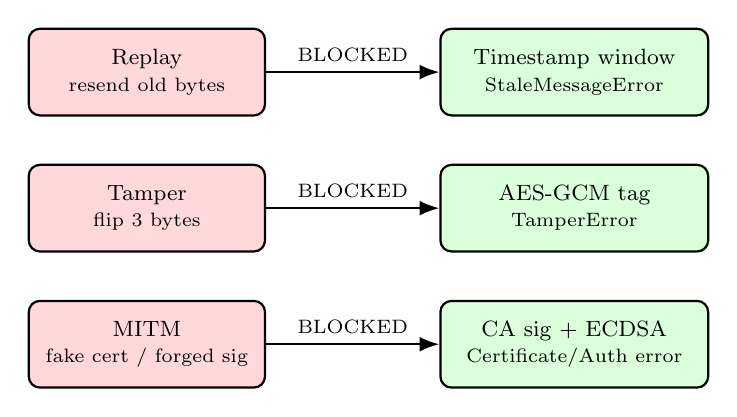
\begin{tikzpicture}[font=\footnotesize,node distance=5mm,
   atk/.style={draw,thick,rounded corners,fill=red!15,minimum width=3.0cm,
               minimum height=1.1cm,align=center},
   def/.style={draw,thick,rounded corners,fill=green!14,minimum width=3.4cm,
               minimum height=1.1cm,align=center}]
  \node[atk] (r) {Replay\\\scriptsize resend old bytes};
  \node[atk,below=6mm of r] (t) {Tamper\\\scriptsize flip 3 bytes};
  \node[atk,below=6mm of t] (m) {MITM\\\scriptsize fake cert / forged sig};
  \node[def,right=22mm of r] (rd) {Timestamp window\\\scriptsize StaleMessageError};
  \node[def,right=22mm of t] (td) {AES-GCM tag\\\scriptsize TamperError};
  \node[def,right=22mm of m] (md) {CA sig + ECDSA\\\scriptsize Certificate/Auth error};
  \draw[-{Latex[length=2.5mm]},thick] (r) -- (rd) node[midway,above,font=\scriptsize]{BLOCKED};
  \draw[-{Latex[length=2.5mm]},thick] (t) -- (td) node[midway,above,font=\scriptsize]{BLOCKED};
  \draw[-{Latex[length=2.5mm]},thick] (m) -- (md) node[midway,above,font=\scriptsize]{BLOCKED};
\end{tikzpicture}
\end{center}

\subsection{Diagram 2 --- the replay attack timeline}
\begin{center}
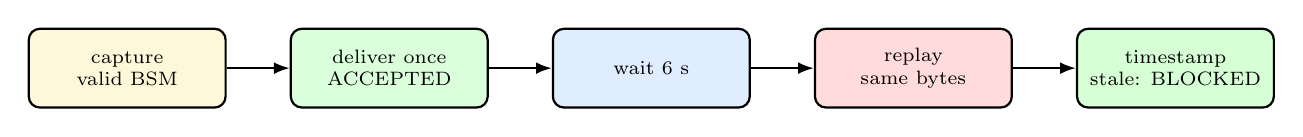
\begin{tikzpicture}[font=\scriptsize,node distance=4mm,
   s/.style={draw,thick,rounded corners,minimum width=2.5cm,minimum height=1.0cm,
             align=center}]
  \node[s,fill=boxyellow] (cap) {capture\\valid BSM};
  \node[s,fill=green!14,right=8mm of cap] (ok) {deliver once\\ACCEPTED};
  \node[s,fill=boxblue,right=8mm of ok] (wait) {wait 6 s};
  \node[s,fill=red!14,right=8mm of wait] (rep) {replay\\same bytes};
  \node[s,fill=green!16,right=8mm of rep] (blk) {timestamp\\stale: BLOCKED};
  \draw[-{Latex[length=2mm]},thick] (cap)--(ok);
  \draw[-{Latex[length=2mm]},thick] (ok)--(wait);
  \draw[-{Latex[length=2mm]},thick] (wait)--(rep);
  \draw[-{Latex[length=2mm]},thick] (rep)--(blk);
\end{tikzpicture}
\end{center}

% =====================================================================
\section{Presentation Pack}
% =====================================================================

\subsection{Slide Outline}

\textbf{Slide 1 --- Why Attack Your Own System?}
\begin{itemize}
  \item A security claim is worthless until tested.
  \item S8 is the project's red team --- three attack scripts.
  \item Each becomes the attacker against the real code.
  \item \texttt{[BLOCKED]} = the defence held; \texttt{[FAIL]} = it broke.
\end{itemize}

\textbf{Slide 2 --- The Replay Attack.}
\begin{itemize}
  \item Capture a valid message, wait 6 seconds, re-send it.
  \item The message is perfectly valid --- just \emph{old}.
  \item Timestamp check: 6\,s $>$ 5\,s $\to$ \texttt{StaleMessageError}.
  \item Result: replay BLOCKED.
\end{itemize}

\textbf{Slide 3 --- The Tamper Attack.}
\begin{itemize}
  \item Encrypt a BSM, flip 3 random bytes in the ciphertext.
  \item AES-GCM tag no longer matches $\to$ \texttt{TamperError}.
  \item The original, untouched message still decrypts fine.
  \item Result: tamper BLOCKED.
\end{itemize}

\textbf{Slide 4 --- The Man-in-the-Middle Attack.}
\begin{itemize}
  \item Scenario A: fake self-signed certificate $\to$ \texttt{CertificateError}.
  \item Scenario B: forged challenge signature $\to$ \texttt{ecdsa\_verify} False.
  \item Attacker lacks the CA key and the vehicle's private key.
  \item Result: both scenarios BLOCKED.
\end{itemize}

\textbf{Slide 5 --- Why the Attacker Always Loses.}
\begin{itemize}
  \item Every attack fails for one reason: a missing secret.
  \item No session key, no CA key, no vehicle private key.
  \item Honest limits: in-process tests, not a live network attack.
  \item The demos prove the crypto, not an exhaustive security proof.
\end{itemize}

\subsection{Speaker Talking Points (about 30--60 seconds each)}

\textbf{Slide 1.} ``It is easy to \emph{say} a system is secure. It means nothing
until someone genuinely tries to break it. Section eight is exactly that --- the
project's red team. There are three scripts, and each one becomes the attacker.
They do not use a watered-down copy of the code; they import the real project
modules and attack them. If a defence failed, the script would print FAIL in
capital letters. Every time, it prints BLOCKED.''

\textbf{Slide 2.} ``First, the replay attack. The attacker records a genuine,
valid, encrypted message. Notice --- nothing is forged here; the message is
completely legitimate. The script delivers it once, and it is accepted, proving
it is valid. Then it waits six seconds and sends the exact same bytes again. Now
the message's timestamp is six seconds old, and our freshness window is five.
secure\_receive raises a StaleMessageError. The replay is blocked --- not because
the message is fake, but because it is old.''

\textbf{Slide 3.} ``Second, the tamper attack. The script encrypts a safety
message, then plays the attacker: it flips three random bytes in the middle of
the packet, in the ciphertext region. Then it tries to receive it. AES-GCM
recomputes its authentication tag, the tag does not match the changed bytes, and
secure\_receive throws a TamperError. To prove the rejection is really caused by
the tampering, the script then decrypts the \emph{original} untouched message ---
and that one works perfectly. Only the tampered copy fails.''

\textbf{Slide 4.} ``Third, the man-in-the-middle, in two flavours. In Scenario A
the attacker builds their own certificate claiming to be vehicle-a. But they
cannot sign it as the CA --- they do not have the CA's key --- so it is
self-signed, and our certificate check raises a CertificateError. In Scenario B
the attacker lets the real certificates through but tries to answer the handshake
challenge by signing the nonces with their own key. When we verify that signature
with vehicle-a's real public key, it returns False. Both scenarios blocked.''

\textbf{Slide 5.} ``Step back and notice the pattern. Every single attack fails
for the same root reason: the attacker is missing a secret. They do not have the
session key, so they cannot tamper. They do not have the CA's key, so they cannot
forge a certificate. They do not have the vehicle's private key, so they cannot
forge a signature. And to be honest about the limits: these scripts run in one
process against the library functions, so they prove the cryptography is sound,
not that the networking is flawless, and they test the specific attacks we chose
rather than every possible attack.''

\subsection{Live-Demo Script}
\begin{enumerate}
  \item \textbf{Replay.} Run \texttt{python attacks\textbackslash
        replay\_attack.py}. Point at \texttt{First delivery ACCEPTED} (valid),
        the 6-second countdown, then \texttt{[BLOCKED] ... Message is 6.0s old}.
  \item \textbf{Tamper.} Run \texttt{python attacks\textbackslash
        tamper\_attack.py}. Point at the three flipped byte positions, then
        \texttt{[BLOCKED] ... auth tag mismatch}, then the original still decrypts.
  \item \textbf{MITM.} Run \texttt{python attacks\textbackslash mitm\_attack.py}
        (certificates must exist). Point at the two \texttt{[BLOCKED]} lines ---
        one for the fake certificate, one for the forged signature.
  \item \textbf{Optional break-it.} Change the replay wait to 3 seconds and show
        the message is now accepted --- explaining the timestamp window.
\end{enumerate}

\subsection{Examiner Q\&A}
\begin{enumerate}
  \item \textbf{Q: Why does the project include attack scripts at all?}\\
        A: To \emph{prove} the defences by adversarial testing. A claimed defence
        is only credible once a real attack against the real code is shown to
        fail.
  \item \textbf{Q: In the replay attack, is the message forged?}\\
        A: No --- it is a genuine, validly encrypted and signed message. The only
        thing wrong is that it is old; the timestamp window catches it.
  \item \textbf{Q: How exactly does the tamper attack get blocked?}\\
        A: Flipping bytes changes the ciphertext; AES-GCM's recomputed
        authentication tag no longer matches, \texttt{aes\_gcm\_decrypt} raises
        \texttt{DecryptionError}, and \texttt{secure\_receive} raises
        \texttt{TamperError}.
  \item \textbf{Q: Why does the tamper script also decrypt the original?}\\
        A: As a control --- it proves the channel works and that the rejection
        was caused specifically by the tampering, not a setup error.
  \item \textbf{Q: What are the two MITM scenarios and what blocks each?}\\
        A: (A) A fake self-signed certificate, blocked by
        \texttt{verify\_certificate\_against\_ca} (no CA signature). (B) A forged
        challenge signature, blocked by \texttt{ecdsa\_verify} with the real
        public key.
  \item \textbf{Q: What single thing does the attacker always lack?}\\
        A: A required secret --- the session key, the CA's private key, or the
        vehicle's private key. Without it, no attack succeeds.
  \item \textbf{Q: A replay within 5 seconds --- would this script catch it?}\\
        A: Not by itself: the timestamp would pass and \texttt{secure\_receive}
        does not consult the nonce cache. Catching that needs the nonce-cache
        layer, which the handshake (S4) uses.
  \item \textbf{Q: Name a limitation of these demonstrations.}\\
        A: They run in one process against library functions, not a live TCP
        connection, and they test chosen attacks --- so they evidence the
        cryptographic defences rather than constitute an exhaustive proof.
\end{enumerate}

% =====================================================================
\section{Glossary}
% =====================================================================
\begin{description}[style=nextline,leftmargin=0pt]
  \item[Adversarial testing] Deliberately attacking your own system to test it.
  \item[Red team] The people (or scripts) that play the attacker.
  \item[Replay attack] Re-sending a previously captured valid message.
  \item[Tamper attack] Changing a message's bytes in transit.
  \item[MITM] Man-in-the-Middle: an attacker secretly between two parties.
  \item[Self-signed certificate] A certificate signed with its own key, not the CA's.
  \item[Forged signature] A signature made with the wrong (attacker's) private key.
  \item[Freshness window] The 5-second age limit on a valid message.
  \item[Authentication tag] The 16-byte AES-GCM value that detects tampering.
  \item[Sequence number] A per-sender counter that must always increase.
  \item[StaleMessageError] Exception for a message older than the window.
  \item[TamperError] Exception for a packet that failed an integrity check.
  \item[CertificateError] Exception when certificate verification fails.
  \item[XOR / \^{}=] The bitwise operation used to flip bits when tampering.
  \item[bytearray] A mutable sequence of bytes (so it can be edited).
  \item[Session key] The shared 32-byte AES key (here simulated for the demos).
  \item[CA] Certificate Authority --- whose private key the attacker lacks.
  \item[Chain of trust] The signature link from a certificate to the trusted CA.
  \item[ecdsa\_verify] The function that returns False for a forged signature.
  \item[verify\_certificate\_against\_ca] The function that rejects a non-CA-signed cert.
\end{description}

% =====================================================================
\section{References and Further Study}
% =====================================================================
\begin{itemize}
  \item \textbf{Replay attack (Wikipedia)} ---
        \url{https://en.wikipedia.org/wiki/Replay_attack}\\
        Read for: how replay works and standard defences.
  \item \textbf{Man-in-the-middle attack (Wikipedia)} ---
        \url{https://en.wikipedia.org/wiki/Man-in-the-middle_attack}\\
        Read for: the MITM concept behind both scenarios.
  \item \textbf{Tampering / message integrity (Wikipedia: Data integrity)} ---
        \url{https://en.wikipedia.org/wiki/Data_integrity}\\
        Read for: why detecting modification matters.
  \item \textbf{Red team (Wikipedia)} ---
        \url{https://en.wikipedia.org/wiki/Red_team}\\
        Read for: the idea of adversarial testing.
  \item \textbf{Penetration test (Wikipedia)} ---
        \url{https://en.wikipedia.org/wiki/Penetration_test}\\
        Read for: professional security testing of which these scripts are a tiny version.
  \item \textbf{OWASP Web Security Testing Guide} ---
        \url{https://owasp.org/www-project-web-security-testing-guide/}\\
        Read for: how real-world security testing is structured.
  \item \textbf{Galois/Counter Mode (Wikipedia)} ---
        \url{https://en.wikipedia.org/wiki/Galois/Counter_Mode}\\
        Read for: why a flipped byte breaks the AES-GCM tag.
  \item \textbf{X.509 (Wikipedia)} ---
        \url{https://en.wikipedia.org/wiki/X.509}\\
        Read for: why a self-signed certificate fails the CA check.
  \item \textbf{Python cryptography --- exceptions} ---
        \url{https://cryptography.io/en/latest/exceptions/}\\
        Read for: \texttt{InvalidSignature} and \texttt{InvalidTag}, the errors
        behind the rejections.
  \item \textbf{MITRE ATT\&CK --- Adversary-in-the-Middle} ---
        \url{https://attack.mitre.org/techniques/T1557/}\\
        Read for: how MITM is catalogued as a real-world technique.
\end{itemize}

\vfill
\begin{center}\footnotesize\itshape
End of Section S8. Next: S9 --- the security evaluation that measures how well
these defences perform.
\end{center}



% ===================== 09-security-evaluation.tex =====================
\chapter{S9 --- Security Evaluation}

\section{Title and ``What You'll Learn''}
% =====================================================================

\subsection*{Section Title}
\textbf{S9 --- Security Evaluation: a script that \emph{measures} the project ---
how fast the cryptography runs and how reliably the defences catch attacks ---
and prints a pass/fail report.}

\subsection*{Plain-English Summary (read this first)}
Section~S8 \emph{proved} the defences work by attacking them once each. Section~S9
goes further: it \emph{measures} them, many times over, and writes the numbers
down. One script, \texttt{evaluate\_security.py}, runs six tests. Three are
\textbf{speed} tests --- can the encryption, decryption and signing keep up with
a car sending messages in real time? Three are \textbf{correctness} tests --- do
the replay and tamper defences catch \emph{100\%} of attacks, and are the random
nonces truly unique? Every test has a numeric \textbf{target}; the script prints
a table of \texttt{PASS} / \texttt{FAIL} and saves it to a report file. S9 is the
\emph{evidence} behind the project's security claims.

\subsection*{Learning Outcomes}
After studying this section you will be able to:
\begin{itemize}
  \item Explain \textbf{benchmarking} and what \textbf{throughput} (ops/second) means.
  \item Explain why a \textbf{high-resolution timer} is used for measurement.
  \item Explain a \textbf{detection rate} and why 100\% is the target.
  \item Explain \textbf{nonce uniqueness} and, briefly, the \emph{birthday problem}.
  \item Walk through all six test functions and the report formatter.
  \item Run the evaluation, read the table, and explain every row.
  \item Explain the difference between \emph{measuring} and \emph{proving} security.
\end{itemize}

% =====================================================================
\section{Where This Fits}
% =====================================================================

S9 sits \emph{above} the whole pipeline as its report card. The earlier sections
\emph{build} the defences and S8 \emph{attacks} them once; S9 \emph{quantifies}
them. It imports the real crypto functions (S3) and the real
\texttt{ReplayCache} (S4) and runs them thousands of times to produce hard
numbers --- both for \emph{performance justification} (``ECDSA and AES are fast
enough for V2V'') and for \emph{security evidence} (``replay and tamper detection
are 100\%'').

\begin{center}
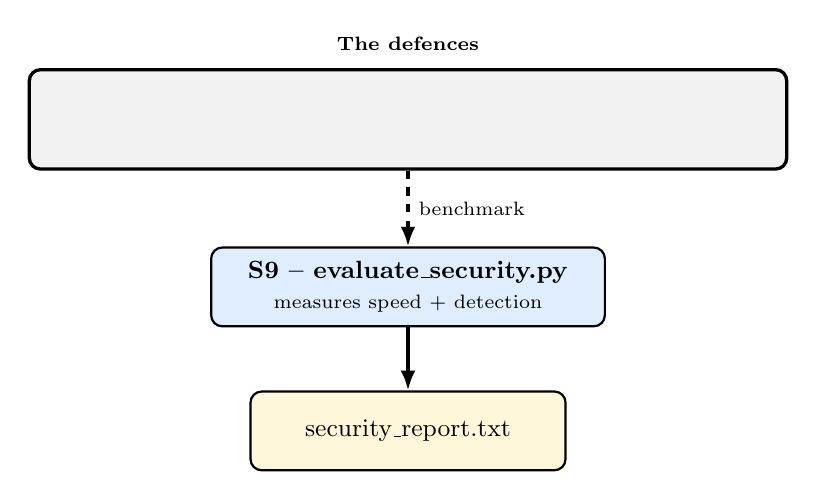
\begin{tikzpicture}[font=\small,node distance=7mm and 9mm,
   st/.style={draw,rounded corners,minimum width=2.5cm,minimum height=1.0cm,
              align=center,thick}]
  \node[st,fill=red!12]   (cr) {Crypto\\\scriptsize S3};
  \node[st,fill=green!12,right=of cr] (au) {Handshake\\\scriptsize S4};
  \node[st,fill=boxyellow,right=of au] (ms) {Messaging\\\scriptsize S5};
  \node[draw,very thick,rounded corners,fill=gray!10,fit=(cr)(au)(ms)] (sys) {};
  \node[above=1mm of sys,font=\scriptsize\bfseries] {The defences};
  \node[st,fill=boxblue,below=11mm of au,minimum width=5cm] (ev)
       {\textbf{S9 -- evaluate\_security.py}\\\scriptsize measures speed + detection};
  \draw[-{Latex[length=2.5mm]},very thick,dashed] (sys) -- (ev)
       node[midway,right,font=\scriptsize]{benchmark};
  \node[st,fill=boxyellow,below=8mm of ev,minimum width=4cm] (rep) {security\_report.txt};
  \draw[-{Latex[length=2.5mm]},very thick] (ev) -- (rep);
\end{tikzpicture}
\end{center}

% =====================================================================
\section{The Theory You Must Study}
% =====================================================================

\subsection{Benchmarking and Throughput}
\textbf{Plain definition.} \emph{Benchmarking} means measuring how fast a piece
of code runs, under controlled, repeatable conditions. \emph{Throughput} is the
amount of work done per unit time --- here, \textbf{operations per second}
(ops/s).

\textbf{Real-life analogy.} Timing how many envelopes a person can seal in one
minute. Do it once and it is a fluke; do it over a thousand envelopes and you
have a trustworthy rate.

\textbf{Why it exists.} A real car sends safety messages many times a second. If
encrypting or signing one message were slow, the security would make the car
\emph{unsafe} by lagging. Benchmarking answers: ``is the cryptography fast enough
for real time?''

\textbf{How it works here.} Each speed test runs an operation in a loop many
times (1000 for encryption/decryption, 100 for signing), measures the total time,
and computes \texttt{ops = iterations / elapsed}.

\textbf{Security property it relates to.} Indirectly all of them --- it shows the
defences are \emph{practical}, not just correct.

\subsection{High-Resolution Timing (\texttt{time.perf\_counter})}
\textbf{Plain definition.} \texttt{time.perf\_counter()} is a clock designed for
measuring short \emph{durations} very precisely.

\textbf{Real-life analogy.} A stopwatch, not a wall clock. A wall clock tells you
the time of day; a stopwatch is built to measure how long something \emph{took}.

\textbf{Why it exists.} An ordinary clock can jump (e.g.\ when the operating
system adjusts the time) and is too coarse for sub-millisecond work.
\texttt{perf\_counter} is steady and fine-grained, so a benchmark is accurate.

\textbf{How it works here.} The pattern is: \texttt{start = time.perf\_counter()},
run the loop, then \texttt{elapsed = time.perf\_counter() - start}.

\textbf{Security property it relates to.} None directly --- it makes the
measurement trustworthy.

\subsection{Pass/Fail Thresholds}
\textbf{Plain definition.} A \emph{threshold} is a fixed target a measurement
must beat to count as a pass.

\textbf{Real-life analogy.} A driving test: parallel-park within a set time or you
fail. The number is decided in advance, so the result is objective.

\textbf{Why it exists.} ``Fast'' and ``reliable'' are vague. A threshold turns a
measurement into a clear yes/no, and makes the report honest --- you cannot move
the goalposts after seeing the result.

\textbf{How it works here.} Encryption and decryption must exceed
\textbf{500 ops/s}; signing must exceed \textbf{100 ops/s}; detection tests must
be \textbf{100\%}; nonce collisions must be \textbf{0}. Each test sets
\texttt{passed = (measurement\ meets\ target)}.

\textbf{Security property it relates to.} It makes every other property
\emph{measurable} rather than asserted.

\subsection{Detection Rate}
\textbf{Plain definition.} A \emph{detection rate} is the fraction of attacks a
defence catches: \emph{caught divided by total}.

\textbf{Real-life analogy.} A metal detector at an airport: if 100 weapons go
through and it catches 100, the detection rate is 100\%. Catching 99 is not good
enough.

\textbf{Why it exists.} Catching an attack ``usually'' is a false comfort --- a
single missed tampered message could cause a crash. The only acceptable target
for these defences is \textbf{100\%}.

\textbf{How it works here.} \texttt{test\_replay\_detection} adds 100 nonces to a
\texttt{ReplayCache}, then re-adds each and counts how many raise
\texttt{ReplayError}; it must be 100/100. \texttt{test\_tamper\_detection}
encrypts 50 messages, flips a byte in each, and counts how many decryptions
raise \texttt{DecryptionError}; it must be 50/50.

\textbf{Security property it relates to.} \textbf{Replay prevention} and
\textbf{integrity}.

\subsection{Nonce Uniqueness and the Birthday Problem}
\textbf{Plain definition.} A \emph{nonce} must never repeat. \emph{Nonce
uniqueness} testing checks that a batch of randomly generated nonces contains no
duplicates (\emph{collisions}). The \emph{birthday problem} is the surprising
fact that collisions become likely much sooner than intuition suggests --- but
only when the pool of possible values is small.

\textbf{Real-life analogy.} In a room of just 23 people, two probably share a
birthday --- because there are only 365 possible days. But if ``birthdays'' could
be any of $2^{256}$ values, you would need an unimaginable crowd before a clash.

\textbf{Why it exists.} If two messages reused a nonce, AES-GCM's security would
break. The test gives empirical confidence that \texttt{os.urandom} is producing
fresh values.

\textbf{How it works here.} \texttt{test\_nonce\_uniqueness} generates 10{,}000
nonces of 32 bytes (256 bits) each, puts them in a \texttt{set} (which discards
duplicates), and checks \texttt{collisions = count - len(set)} is 0. With 256-bit
values, 10{,}000 draws colliding is so unlikely it is effectively impossible ---
so a result of 0 is expected every run.

\textbf{Security property it relates to.} It underpins \textbf{confidentiality}
(AES-GCM relies on unique nonces).

\subsection{Measuring vs Proving Security}
\textbf{An important distinction.} S9 \emph{measures}; it does not mathematically
\emph{prove}. A 100\% detection rate over 100 trials is strong \emph{evidence},
but it is not a proof that the defence can \emph{never} fail. Real security
assurance combines testing (like S9), code review, and reasoning about the
underlying mathematics. Being clear about this is part of doing evaluation
honestly --- the script produces a \emph{report}, not a \emph{theorem}.

% =====================================================================
\section{Code Walkthrough}
% =====================================================================

\texttt{evaluate\_security.py} has a header helper, six test functions, a table
formatter, and a \texttt{main} that runs everything and saves a report.

\subsection{The three speed tests}
\begin{lstlisting}[style=py,caption={evaluate\_security.py --- a representative speed benchmark.}]
def test_encryption_speed(iterations: int = 1000) -> dict:
    """Benchmark AES-256-GCM encryption throughput."""
    key = os.urandom(32)
    payload = b"test BSM payload " * 10           # ~170 bytes (realistic BSM)

    start = time.perf_counter()
    for _ in range(iterations):
        aes_gcm_encrypt(key, payload)
    elapsed = time.perf_counter() - start

    ops = iterations / elapsed
    passed = ops > 500
    return {"name": "Encryption Speed", "result": f"{ops:.0f} ops/s",
            "target": ">500", "passed": passed}
\end{lstlisting}
\textbf{Step by step:}
\begin{enumerate}
  \item Make a 32-byte AES key and a ~170-byte payload (about the size of a real
        BSM).
  \item Read the high-resolution clock into \texttt{start}.
  \item Run \texttt{aes\_gcm\_encrypt} 1000 times in a loop.
  \item Read the clock again; \texttt{elapsed} is the total time.
  \item \texttt{ops = iterations / elapsed} is the throughput in operations per
        second.
  \item \texttt{passed} is \texttt{True} if \texttt{ops} beats the 500 ops/s
        threshold.
  \item Return a small dictionary with the name, result, target and pass flag.
\end{enumerate}
\texttt{test\_decryption\_speed} is identical but times \texttt{aes\_gcm\_decrypt}
(it encrypts once first to get something to decrypt). \texttt{test\_signature\_speed}
times \texttt{ecdsa\_sign} over 100 iterations with a target of 100 ops/s ---
signing is slower than symmetric encryption, so it has a lower bar.
\textbf{Theory link:} benchmarking; throughput; \texttt{perf\_counter};
thresholds.

\subsection{test\_replay\_detection() --- 100\% replay catching}
\begin{lstlisting}[style=py,caption={evaluate\_security.py --- the replay detection test.}]
def test_replay_detection(count: int = 100) -> dict:
    cache = ReplayCache(window_seconds=300)
    nonces = [os.urandom(32).hex() for _ in range(count)]
    for n in nonces:
        cache.check_and_add(n)              # first time: accepted

    caught = 0
    for n in nonces:
        try:
            cache.check_and_add(n)          # second time: must be rejected
        except ReplayError:
            caught += 1

    passed = caught == count
    return {"name": "Replay Detection Rate", "result": f"{caught}/{count}",
            "target": "100%", "passed": passed}
\end{lstlisting}
\textbf{Step by step:}
\begin{enumerate}
  \item Create a \texttt{ReplayCache} and generate 100 unique random nonces.
  \item Add each nonce once --- all are new, so all are accepted.
  \item Try to add every nonce a \emph{second} time. Each repeat \emph{must}
        raise \texttt{ReplayError}; \texttt{caught} counts how many do.
  \item The test passes only if \texttt{caught == 100} --- a 100\% detection rate.
\end{enumerate}
\textbf{Theory link:} detection rate; the \texttt{ReplayCache} of S4. This is the
quantified version of the S8 replay attack --- not one replay, but 100.

\subsection{test\_tamper\_detection() --- 100\% tamper catching}
\begin{lstlisting}[style=py,caption={evaluate\_security.py --- the tamper detection test.}]
def test_tamper_detection(count: int = 50) -> dict:
    key = os.urandom(32)
    caught = 0
    for _ in range(count):
        ct, nonce, tag = aes_gcm_encrypt(key, b"test BSM payload " * 10)
        tampered = bytearray(ct)
        if tampered:
            tampered[len(tampered) // 2] ^= 0x01      # flip one bit
        try:
            aes_gcm_decrypt(key, bytes(tampered), nonce, tag)
        except DecryptionError:
            caught += 1
    passed = caught == count
    return {"name": "Tamper Detection Rate", "result": f"{caught}/{count}",
            "target": "100%", "passed": passed}
\end{lstlisting}
\textbf{Step by step:}
\begin{enumerate}
  \item For each of 50 rounds: encrypt a payload, then flip \emph{one bit}
        (\texttt{\^{}= 0x01}) in the middle of the ciphertext.
  \item Try to decrypt the tampered ciphertext. AES-GCM's tag will not match, so
        \texttt{aes\_gcm\_decrypt} raises \texttt{DecryptionError};
        \texttt{caught} is incremented.
  \item The test passes only if all 50 tampered messages were caught --- 50/50.
\end{enumerate}
\textbf{Theory link:} detection rate; AES-GCM integrity (S3). Note it flips just
\emph{one bit} --- the smallest possible change --- and even that is always
caught.

\subsection{test\_nonce\_uniqueness() --- no collisions}
\begin{lstlisting}[style=py,caption={evaluate\_security.py --- the nonce uniqueness test.}]
def test_nonce_uniqueness(count: int = 10000) -> dict:
    nonces = set()
    for _ in range(count):
        nonces.add(os.urandom(32).hex())
    collisions = count - len(nonces)
    passed = collisions == 0
    return {"name": f"Nonce Uniqueness ({count//1000}k)",
            "result": f"{collisions} collisions", "target": "0", "passed": passed}
\end{lstlisting}
\textbf{Step by step:}
\begin{enumerate}
  \item Generate 10{,}000 random 32-byte nonces, adding each to a \texttt{set}.
  \item A \texttt{set} automatically discards duplicates, so if any nonce
        repeated, \texttt{len(nonces)} would be less than \texttt{count}.
  \item \texttt{collisions = count - len(nonces)} --- expected to be 0.
  \item The test passes if there were zero collisions.
\end{enumerate}
\textbf{Theory link:} nonce uniqueness; the birthday problem. With 256-bit
nonces, 10{,}000 draws colliding is astronomically unlikely.

\subsection{format\_table() and main()}
\texttt{format\_table} takes the list of result dictionaries and draws a neat
ASCII table with columns \emph{Test}, \emph{Result}, \emph{Target},
\emph{Status}, then an ``Overall: X/Y tests PASSED'' line. \texttt{main} calls
all six test functions, prints the table, and writes it (with a timestamp) to
\texttt{tests/security\_report.txt} so there is a saved record.

% =====================================================================
\section{Hands-On / Practical}
% =====================================================================

\subsection{Run the evaluation}
\begin{lstlisting}[style=term]
python tests\evaluate_security.py
\end{lstlisting}

\noindent\textbf{Expected output (sample --- speed numbers vary by computer):}
\begin{lstlisting}[style=term]
========================================================
     V2V SECURITY EVALUATION REPORT
========================================================

+-----------------------------+----------------+----------+----------+
| Test                        | Result         | Target   | Status   |
+=============================+================+==========+==========+
| Encryption Speed            | 121840 ops/s   | >500     | PASS     |
| Decryption Speed            | 118905 ops/s   | >500     | PASS     |
| Signature Speed             | 6730 ops/s     | >100     | PASS     |
| Replay Detection Rate       | 100/100        | 100%     | PASS     |
| Tamper Detection Rate       | 50/50          | 100%     | PASS     |
| Nonce Uniqueness (10k)      | 0 collisions   | 0        | PASS     |
+-----------------------------+----------------+----------+----------+

Overall: 6/6 tests PASSED

Report saved to: tests/security_report.txt
\end{lstlisting}

\subsection{What each row means}
\begin{itemize}
  \item \textbf{Encryption / Decryption Speed} --- tens of thousands of
        operations per second, far above the 500 needed; AES-256-GCM is
        comfortably fast enough for a car sending one BSM per second.
  \item \textbf{Signature Speed} --- a few thousand signings per second; ECDSA is
        slower than symmetric encryption (it is public-key maths) but still well
        past its 100 ops/s bar.
  \item \textbf{Replay Detection Rate 100/100} --- every one of 100 repeated
        nonces was caught by the \texttt{ReplayCache}.
  \item \textbf{Tamper Detection Rate 50/50} --- every one-bit change in 50
        messages was caught by AES-GCM.
  \item \textbf{Nonce Uniqueness 0 collisions} --- 10{,}000 random nonces, all
        distinct.
  \item \textbf{Overall 6/6} --- every test met its target.
\end{itemize}

\subsection{Try This Yourself (mini-experiment)}
Open \texttt{evaluate\_security.py} and make the encryption threshold
deliberately impossible:
\begin{lstlisting}[style=term]
passed = ops > 500        ->        passed = ops > 99999999
\end{lstlisting}
\textbf{Predict before you run.} No ordinary computer encrypts 100~million times
a second, so \texttt{ops} will not beat the new bar. Prediction: the Encryption
Speed row now shows \texttt{FAIL}, and the summary changes to \texttt{Overall:
5/6 tests PASSED}. This shows the threshold is what turns a raw number into a
pass/fail verdict --- and why thresholds must be chosen \emph{before} seeing the
result, not after. \textbf{Restore the line to \texttt{> 500} afterwards.}

% =====================================================================
\section{Attack Relevance}
% =====================================================================

S9 does not block any attack itself --- it \emph{quantifies} how well the other
sections block attacks, turning the project's security claims into measured
evidence.

\begin{table}[h]
\centering
\small
\begin{tabular}{@{}p{3.6cm} p{4.2cm} p{4.6cm}@{}}
\toprule
\textbf{S9 test} & \textbf{Attack it relates to} & \textbf{What it evidences}\\
\midrule
Replay Detection Rate & Replay attack (S8). & The \texttt{ReplayCache} of S4
catches 100\% of repeated nonces.\\
Tamper Detection Rate & Tamper attack (S8). & AES-256-GCM (S3) catches 100\% of
one-bit changes.\\
Nonce Uniqueness & Nonce-reuse weakening of AES-GCM. & \texttt{os.urandom}
produces no duplicate nonces.\\
Speed tests & (Not an attack.) & The defences are fast enough for real-time V2V
--- security does not make the car unsafe.\\
\bottomrule
\end{tabular}
\caption{S9 turns S8's one-off demonstrations into measured, repeatable evidence.}
\end{table}

\noindent\textbf{Why the speed tests are a security matter too.} If signing or
encrypting a message were slow, a real car could not keep up with the safety
message rate --- the security layer would itself create a hazard. By showing the
cryptography runs thousands to tens of thousands of times per second, S9
demonstrates the defences are \emph{deployable}, not merely correct.

\textbf{Honest scope note.} S9 is \emph{measurement}, not \emph{proof}. A 100\%
detection rate over 100 or 50 trials is strong evidence but not a guarantee for
every conceivable input. The tests also exercise the cryptographic functions in
isolation --- they do not benchmark the full networked system under load. And the
thresholds (500, 100) are project-chosen reference points, not formal V2V
standards. A complete security assurance would add code review and mathematical
reasoning to this measurement.

% =====================================================================
\section{Illustrations}
% =====================================================================

\subsection{Diagram 1 --- the six tests feeding one report}
\begin{center}
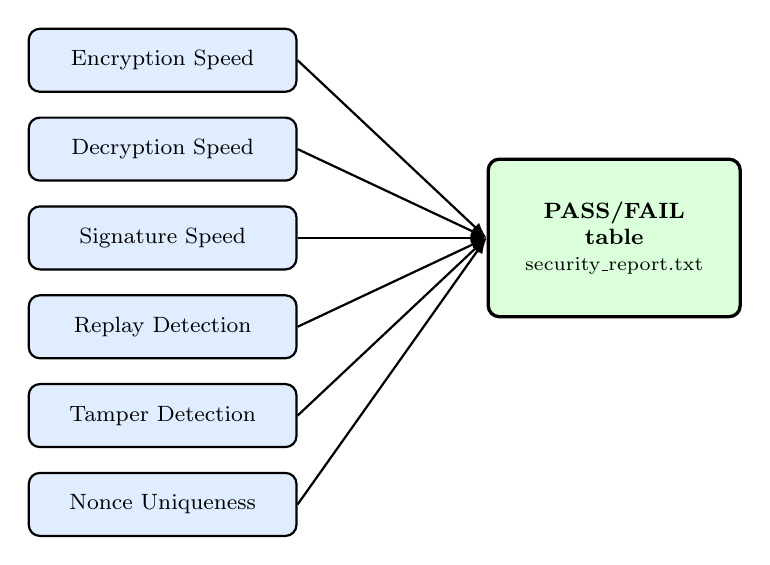
\begin{tikzpicture}[font=\footnotesize,node distance=3mm,
   t/.style={draw,thick,rounded corners,minimum width=3.4cm,minimum height=0.8cm,
             align=center,fill=boxblue}]
  \node[t] (t1) {Encryption Speed};
  \node[t,below=of t1] (t2) {Decryption Speed};
  \node[t,below=of t2] (t3) {Signature Speed};
  \node[t,below=of t3] (t4) {Replay Detection};
  \node[t,below=of t4] (t5) {Tamper Detection};
  \node[t,below=of t5] (t6) {Nonce Uniqueness};
  \node[draw,very thick,rounded corners,fill=green!14,minimum width=3.2cm,
        minimum height=2.0cm,align=center,right=24mm of t3] (rep)
       {\textbf{PASS/FAIL}\\\textbf{table}\\\scriptsize security\_report.txt};
  \foreach \n in {t1,t2,t3,t4,t5,t6}
     \draw[-{Latex[length=2mm]},thick] (\n.east) -- (rep.west);
\end{tikzpicture}
\end{center}

\subsection{Diagram 2 --- the benchmark loop}
\begin{center}
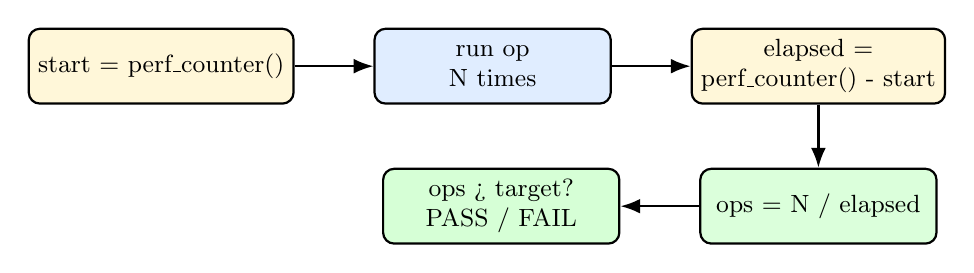
\begin{tikzpicture}[font=\small,node distance=8mm,
   s/.style={draw,thick,rounded corners,minimum width=3.0cm,minimum height=0.95cm,
             align=center}]
  \node[s,fill=boxyellow] (st) {start = perf\_counter()};
  \node[s,fill=boxblue,right=10mm of st] (lp) {run op\\N times};
  \node[s,fill=boxyellow,right=10mm of lp] (en) {elapsed =\\perf\_counter() - start};
  \node[s,fill=green!14,below=8mm of en] (ops) {ops = N / elapsed};
  \node[s,fill=green!16,left=10mm of ops] (cmp) {ops > target?\\PASS / FAIL};
  \draw[-{Latex[length=2.5mm]},thick] (st) -- (lp);
  \draw[-{Latex[length=2.5mm]},thick] (lp) -- (en);
  \draw[-{Latex[length=2.5mm]},thick] (en) -- (ops);
  \draw[-{Latex[length=2.5mm]},thick] (ops) -- (cmp);
\end{tikzpicture}
\end{center}

% =====================================================================
\section{Presentation Pack}
% =====================================================================

\subsection{Slide Outline}

\textbf{Slide 1 --- Why Measure?}
\begin{itemize}
  \item S8 proved the defences once; S9 measures them at scale.
  \item One script, \texttt{evaluate\_security.py}, six tests.
  \item Three speed tests, three correctness tests.
  \item Output: a PASS/FAIL table saved to a report file.
\end{itemize}

\textbf{Slide 2 --- The Speed Tests.}
\begin{itemize}
  \item Encryption, decryption, signing --- measured in ops/second.
  \item A high-resolution timer (\texttt{perf\_counter}) for accuracy.
  \item Targets: $>$500 ops/s for AES, $>$100 ops/s for ECDSA.
  \item Question answered: ``fast enough for real-time V2V?''
\end{itemize}

\textbf{Slide 3 --- The Detection Tests.}
\begin{itemize}
  \item Replay: re-add 100 nonces --- all 100 must be rejected.
  \item Tamper: flip one bit in 50 messages --- all 50 must fail to decrypt.
  \item Target for both: 100\%. Anything less is a fail.
  \item These quantify the S3 and S4 defences.
\end{itemize}

\textbf{Slide 4 --- Nonce Uniqueness.}
\begin{itemize}
  \item Generate 10{,}000 random 256-bit nonces.
  \item Put them in a set; count duplicates.
  \item Target: 0 collisions --- AES-GCM needs unique nonces.
  \item 256-bit values make a collision effectively impossible.
\end{itemize}

\textbf{Slide 5 --- Measuring is Not Proving.}
\begin{itemize}
  \item 6/6 PASS is strong evidence the design holds.
  \item But a test is a sample, not a mathematical proof.
  \item Honest assurance also needs review and reasoning.
  \item S9 produces a \emph{report card}, not a \emph{theorem}.
\end{itemize}

\subsection{Speaker Talking Points (about 30--60 seconds each)}

\textbf{Slide 1.} ``In the previous section we proved each defence works by
attacking it once. Section nine is the next step: instead of one attack, we
\emph{measure}. One script, evaluate\_security.py, runs six tests. Three of them
check speed --- is the cryptography fast enough? --- and three check correctness
--- do the defences catch every attack, and are the random values truly unique?
At the end it prints a clean pass-or-fail table and even saves it to a report
file, so there is a permanent record.''

\textbf{Slide 2.} ``The three speed tests run an operation in a tight loop ---
encrypting a thousand times, signing a hundred times --- and measure how long it
took with a high-resolution stopwatch called perf\_counter. Dividing the count by
the time gives operations per second. Why does this matter for security? Because
a real car sends safety messages constantly. If encryption were slow, the
security layer would make the car lag, which is itself dangerous. We set targets
in advance --- five hundred operations a second for encryption, a hundred for
signing --- and the real numbers beat them easily.''

\textbf{Slide 3.} ``The detection tests quantify the defences. The replay test
adds a hundred nonces to the cache, then tries to add every one again --- and all
one hundred repeats must be rejected. The tamper test encrypts fifty messages,
flips a single bit in each, and every one of the fifty must fail to decrypt. The
target for both is one hundred percent, and that is deliberate. Catching
ninety-nine attacks out of a hundred is not good enough when the one you miss
could be a false `I am braking' that causes a crash.''

\textbf{Slide 4.} ``The sixth test checks nonce uniqueness. Remember a nonce must
never repeat, or AES-GCM's security breaks. The test generates ten thousand
random nonces and drops them into a set, which automatically removes duplicates.
If the set still has ten thousand items, there were no collisions. And because
each nonce is 256 bits long, the chance of a clash is astronomically small ---
this is the birthday problem, but with so many possible values that a collision
is effectively impossible.''

\textbf{Slide 5.} ``One honest closing point. A result of six out of six is
genuinely strong evidence that the design holds up. But a test runs a sample of
inputs --- it is not a mathematical proof that the defence can never fail under
any input. Real-world security assurance combines testing like this with careful
code review and reasoning about the underlying cryptographic mathematics. So
think of section nine as the project's report card --- convincing evidence ---
rather than a final theorem.''

\subsection{Live-Demo Script}
\begin{enumerate}
  \item \textbf{Run it.} Execute \texttt{python tests\textbackslash
        evaluate\_security.py}.
  \item \textbf{Point at the speed rows.} ``Tens of thousands of operations a
        second --- far past the target. The cryptography is fast enough.''
  \item \textbf{Point at the detection rows.} \texttt{100/100} and \texttt{50/50}
        --- ``every single attack caught.''
  \item \textbf{Point at the summary.} \texttt{Overall: 6/6 tests PASSED}.
  \item \textbf{Show the saved report.} Open \texttt{tests\textbackslash
        security\_report.txt} --- ``a permanent, timestamped record.''
  \item \textbf{Optional break-it.} Raise the encryption threshold absurdly high
        and re-run to show a \texttt{FAIL} and \texttt{5/6}.
\end{enumerate}

\subsection{Examiner Q\&A}
\begin{enumerate}
  \item \textbf{Q: What is the purpose of \texttt{evaluate\_security.py}?}\\
        A: To measure the project --- the speed of the cryptography and the
        reliability of the defences --- and produce a pass/fail evidence report.
  \item \textbf{Q: What is throughput and why is it measured here?}\\
        A: Operations per second. It shows the cryptography is fast enough for a
        car sending safety messages in real time, so security does not cause
        dangerous lag.
  \item \textbf{Q: Why use \texttt{time.perf\_counter} rather than an ordinary clock?}\\
        A: \texttt{perf\_counter} is a high-resolution, steady stopwatch built
        for measuring short durations; a wall clock can jump and is too coarse.
  \item \textbf{Q: Why must the detection rate target be 100\%?}\\
        A: A single missed tampered or replayed safety message could cause a
        crash. For these defences, anything below 100\% is unacceptable.
  \item \textbf{Q: How does the tamper test work?}\\
        A: It encrypts 50 messages, flips one bit of ciphertext in each, and
        counts how many decryptions raise \texttt{DecryptionError}. All 50 must.
  \item \textbf{Q: What is the nonce uniqueness test checking, and why does it
        pass?}\\
        A: That 10{,}000 random nonces contain no duplicates. Because each nonce
        is 256 bits, a collision is astronomically unlikely (the birthday problem
        with a vast value space), so 0 collisions is expected.
  \item \textbf{Q: Where do the thresholds 500 and 100 come from?}\\
        A: They are project-chosen reference targets, set in advance so the
        verdict is objective. They are not formal V2V standards.
  \item \textbf{Q: Does a 6/6 pass \emph{prove} the system is secure?}\\
        A: No. It is strong \emph{evidence} from a sample of inputs, not a
        mathematical proof. Full assurance also needs code review and reasoning
        about the cryptography.
\end{enumerate}

% =====================================================================
\section{Glossary}
% =====================================================================
\begin{description}[style=nextline,leftmargin=0pt]
  \item[Security evaluation] Measuring how well a system's defences perform.
  \item[Benchmarking] Measuring code speed under controlled, repeatable conditions.
  \item[Throughput] Work done per unit time --- here operations per second (ops/s).
  \item[Operation] One run of a function being measured (one encrypt, one sign...).
  \item[time.perf\_counter] A high-resolution timer for measuring durations.
  \item[Iteration] One pass of a benchmark loop.
  \item[Threshold / target] The fixed value a measurement must beat to pass.
  \item[Pass / Fail] The verdict from comparing a measurement to its threshold.
  \item[Detection rate] Fraction of attacks a defence catches (caught / total).
  \item[Replay detection] Catching repeated nonces (tested via \texttt{ReplayCache}).
  \item[Tamper detection] Catching modified ciphertext (tested via AES-GCM).
  \item[Nonce] A value that must be used only once.
  \item[Collision] Two generated values turning out to be identical.
  \item[Nonce uniqueness] The property that generated nonces never repeat.
  \item[Birthday problem] Why collisions appear sooner than expected --- but only
        with a small value space.
  \item[set] A Python collection that automatically discards duplicates.
  \item[ReplayCache] The S4 class storing seen nonces; tested here.
  \item[DecryptionError] The exception AES-GCM raises on a tampered message.
  \item[ReplayError] The exception the ReplayCache raises on a repeated nonce.
  \item[security\_report.txt] The saved file holding the evaluation results.
  \item[Evidence vs proof] Tests give evidence; only mathematics gives proof.
\end{description}

% =====================================================================
\section{References and Further Study}
% =====================================================================
\begin{itemize}
  \item \textbf{Python time module --- \texttt{perf\_counter}} ---
        \url{https://docs.python.org/3/library/time.html#time.perf_counter}\\
        Read for: the high-resolution timer used in every speed test.
  \item \textbf{Python set type documentation} ---
        \url{https://docs.python.org/3/library/stdtypes.html#set}\\
        Read for: how the nonce-uniqueness test discards duplicates.
  \item \textbf{Benchmark (computing) (Wikipedia)} ---
        \url{https://en.wikipedia.org/wiki/Benchmark_(computing)}\\
        Read for: what benchmarking is and how to do it fairly.
  \item \textbf{Throughput (Wikipedia)} ---
        \url{https://en.wikipedia.org/wiki/Throughput}\\
        Read for: the operations-per-second idea.
  \item \textbf{Birthday problem (Wikipedia)} ---
        \url{https://en.wikipedia.org/wiki/Birthday_problem}\\
        Read for: why collisions appear sooner than intuition suggests.
  \item \textbf{Birthday attack (Wikipedia)} ---
        \url{https://en.wikipedia.org/wiki/Birthday_attack}\\
        Read for: the cryptographic version --- why nonce/hash sizes matter.
  \item \textbf{Cryptographic nonce (Wikipedia)} ---
        \url{https://en.wikipedia.org/wiki/Cryptographic_nonce}\\
        Read for: why nonce uniqueness is essential to AES-GCM.
  \item \textbf{NIST SP 800-38D --- AES-GCM} ---
        \url{https://csrc.nist.gov/pubs/sp/800/38/d/final}\\
        Read for: the official nonce rule the uniqueness test supports.
  \item \textbf{Python os.urandom documentation} ---
        \url{https://docs.python.org/3/library/os.html#os.urandom}\\
        Read for: the source of the random nonces being tested.
  \item \textbf{Software testing (Wikipedia)} ---
        \url{https://en.wikipedia.org/wiki/Software_testing}\\
        Read for: the broader idea that testing gives evidence, not proof.
\end{itemize}

\vfill
\begin{center}\footnotesize\itshape
End of Section S9 --- and of the V2V study pack (S1--S9). The evaluation report
is the project's final evidence that all six security properties hold.
\end{center}


\end{document}
